\documentclass[a5paper, 12pt, openany]{book} % A5 paper size

% \usepackage[paperwidth=148mm, paperheight=210mm, top=1.27cm, bottom=1.27cm, inner=1.9cm, outer=1.27cm, headsep=1.5cm, footskip=1.75cm]{geometry} % Custom dimensions and margins
% Adjusted margins to ensure space for page numbers
\usepackage[paperwidth=148mm, paperheight=210mm, 
         top=1.27cm, bottom=2.5cm, inner=2.2cm, outer=1.27cm, 
         headsep=1.5cm, footskip=1.5cm]{geometry}


\usepackage[utf8]{inputenc}
\usepackage{ctex}

\usepackage{fancyhdr}
\pagestyle{fancy}
\fancyhf{} % Clear all header and footer fields
% \fancyfoot[C]{\thepage} % Center the page number at the bottom
% Define left and right page numbering
\fancyfoot[LE]{\thepage} % Left side for even pages
\fancyfoot[RO]{\thepage} % Right side for odd pages
% Ensure the chapter pages (plain style) also have this layout
\makeatletter
\let\ps@plain\ps@fancy
\makeatother



% *-----------------------------------------------------------------------*
% | Fonts and typography                                                  |
% *-----------------------------------------------------------------------*

% Set CJK main font (for Chinese/Japanese/Korean characters)

% \setmainfont{Times New Roman}
\setCJKmainfont{BabelStone Han}
% doesn't work
% \setCJKmainfont{JyutcitziWithSourceHanSerifTCRegular}[
% Renderer=Basic,
% UprightFont = * ,
% FallbackFonts={BabelStone Han}
% ]



% You can also use \newfontfamily for custom non-CJK fonts if needed
% \setCJKmainfont{JyutcitziWithPMingLiURegular}[Path = ./, Extension = .ttf]
% \setCJKmainfont{JyutcitziWithSourceHanSerifTCRegular}[Path = ./, Extension = .ttf]



\newfontfamily{\jczPMingLiU}{JyutcitziWithPMingLiURegular}[Path = ./fonts/, Extension = .ttf]
% This has the best rendition for latin characters 
\newfontfamily{\jcz}{JyutcitziWithSourceHanSerifTCRegular}[Path = ./fonts/, Extension = .ttf]
\newfontfamily{\batang}{batang}[Path = ./fonts/, Extension = .ttf]
\newCJKfontfamily\koreanfont{Batang}[Path = ./fonts/, Extension = .ttf]
\newfontfamily{\taigi}{GentiumBookPlus-Regular}[Path = ./fonts/, Extension = .ttf]





% *-----------------------------------------------------------------------*
% | Formatting     |
% *-----------------------------------------------------------------------*
% Set global paragraph indentation and spacing
\setlength{\parindent}{2em} % Adjust this value for the desired indentation
\setlength{\parskip}{0pt}   % No space between paragraphs

% for quotes
\usepackage{epigraph} 


\makeatletter
\renewcommand{\@makefntext}[1]{\jcz{\@thefnmark.} #1}
\makeatother
% to control itemise spacing
\usepackage{enumitem}



% *-----------------------------------------------------------------------*
% | Math & Equations     |
% *-----------------------------------------------------------------------*
\usepackage{amsmath} % For advanced math formatting
\usepackage{amssymb} % For mathematical symbols
% \usepackage{tikz} % For drawing logic decision trees


% *-----------------------------------------------------------------------*
% | Table Management                                                      |
% *-----------------------------------------------------------------------*


\usepackage{graphicx}
\usepackage{array}
\usepackage{tabularx}
\usepackage{tabularray}

\usepackage{float}      % Add the float package
\usepackage{longtable}


\usepackage[table,xcdraw]{xcolor}
% 

% Load ruby package for furigana (Ruby text)
\usepackage{ruby}
% \renewcommand{\ruby}[2]{%
%   \ruby{\jcz{#1}}{\jcz{#2}}%
% }


% *-----------------------------------------------------------------------*
% | Chinese and Soochow Numerals               |
% *-----------------------------------------------------------------------*

% Define Chinese numerals for numbers 1-99
% 〇〡〢 〣 〤 〥 〦 〧 〨 〩 十 〹 〺 卅
% Include the numerals file
% numerals.tex
% Define Chinese and Soochow numerals for chapter management

\newcommand{\soochowNumeral}[1]{%
  \ifnum#1<10
    \ifcase#1 〇\or 〡\or 〢\or 〣\or 〤\or 〥\or 〦\or 〧\or 〨\or 〩\fi%
  \else
    \ifnum#1<20
      〸\soochowUnits{\numexpr#1-10\relax}%
    \else
      \ifnum#1<30
        〹\soochowUnits{\numexpr#1-20\relax}%
      \else
        \ifnum#1<40
          〺\soochowUnits{\numexpr#1-30\relax}%
        \else
          \ifnum#1<50
            卅\soochowUnits{\numexpr#1-40\relax}%
          \else
            \ifnum#1<60
              〥十\soochowUnits{\numexpr#1-50\relax}%
            \else
              \ifnum#1<70
                〦十\soochowUnits{\numexpr#1-60\relax}%
              \else
                \ifnum#1<80
                  〧十\soochowUnits{\numexpr#1-70\relax}%
                \else
                  \ifnum#1<90
                    〨十\soochowUnits{\numexpr#1-80\relax}%
                  \else
                    \ifnum#1<100
                      〩十\soochowUnits{\numexpr#1-90\relax}%
                    \fi
                  \fi
                \fi
              \fi
            \fi
          \fi
        \fi
      \fi
    \fi
  \fi
}

\newcommand{\soochowUnits}[1]{%
  \ifnum#1=0
  \else
    \ifnum#1<4
      \ifcase#1 \or 一\or 二\or 三\fi%
    \else
      \soochowNumeral{#1}
    \fi
  \fi
}

\newcommand{\chinesenumeral}[1]{%
  \ifnum#1<10
    \ifcase#1 〇\or 一\or 二\or 三\or 四\or 五\or 六\or 七\or 八\or 九\fi%
  \else
    \ifnum#1<20
      十\chinesenumeral{\numexpr#1-10\relax}%
    \else
      \ifnum#1<30
        二十\chinesenumeral{\numexpr#1-20\relax}%
      \else
        \ifnum#1<40
          三十\chinesenumeral{\numexpr#1-30\relax}%
        \else
          \ifnum#1<50
            四十\chinesenumeral{\numexpr#1-40\relax}%
          \else
            \ifnum#1<60
              五十\chinesenumeral{\numexpr#1-50\relax}%
            \else
              \ifnum#1<70
                六十\chinesenumeral{\numexpr#1-60\relax}%
              \else
                \ifnum#1<80
                  七十\chinesenumeral{\numexpr#1-70\relax}%
                \else
                  \ifnum#1<90
                    八十\chinesenumeral{\numexpr#1-80\relax}%
                  \else
                    \ifnum#1<100
                      九十\chinesenumeral{\numexpr#1-90\relax}%
                    \fi
                  \fi
                \fi
              \fi
            \fi
          \fi
        \fi
      \fi
    \fi
  \fi
}


% *-----------------------------------------------------------------------*
% | Table of contents & Chapter for chapter management |
% *-----------------------------------------------------------------------*

\renewcommand{\figurename}{圗} % So figures would be labeled with 圗 instead of "figure"

% * * * Now for the table of contents
\renewcommand{\contentsname}{目錄} % Traditional Chinese characters for "Contents"
\setcounter{secnumdepth}{0} % no numbering for sections 
% Increase chapter title size in TOC
\usepackage{tocloft} % For customizing table of contents
\renewcommand{\cftchapfont}{\Large\bfseries} % Large and bold chapter titles
\renewcommand{\cftchappagefont}{\Large\bfseries} % Large and bold page numbers
\renewcommand{\cftchapnumwidth}{3em} % Adjust the width for chapter numbers (increase the space)

% Custom chapter numbering in the TOC with Soochow numerals
\renewcommand{\cftchapleader}{\cftdotfill{\cftsecdotsep}} % Dotted line between chapter and page number
\renewcommand{\cftchapaftersnum}{\quad} % Space between Soochow numeral and chapter title

% Redefine how chapter numbers are displayed in the TOC using Soochow numerals
\makeatletter
\renewcommand{\cftchapleader}{\cftdotfill{\cftsecdotsep}} % Dotted line between chapter and page number
\renewcommand{\cftchapaftersnum}{\quad} % Space between Soochow numeral and chapter title
% comment this out if you don't want to use the soochow numerlas
\renewcommand{\numberline}[1]{\soochowNumeral{#1}\hspace{1em}} % Use Soochow numerals for TOC chapter numbers
\makeatother


% create index - run \makeindex in the document
\usepackage{makeidx}
\makeindex



% % Custom chapter title formatting with Chinese numeral chapter numbers
\usepackage{titlesec}

% Custom chapter title formatting with Chinese numeral chapter numbers
\titleformat{\chapter}[block] % 'block' means the title appears on a new line
  {\Huge\bfseries} % Font size and bold formatting for the title
  {\soochowNumeral{\thechapter}} % Chinese character for chapter number
  {1em} % Space between the number and the title
  {\Huge} % Custom style for the chapter title itself (can modify)

% Remove the default LaTeX behavior of forcing new chapters to start on a new page
\makeatletter
\renewcommand\chapter{\if@openright\cleardoublepage\else\clearpage\fi
  \thispagestyle{plain}%
  \global\@topnum\z@
  \@afterindentfalse
  \secdef\@chapter\@schapter}
\makeatother






% *-----------------------------------------------------------------------*
\begin{document}
% to avoid overfull hbox
\sloppy
% % \jcz{} must be run so the document can process jyutcitzi 
\jcz{} 


% % \jczSourceHan{}

\tableofcontents
\newpage
% \chapterwithtoc{Introduction}

聲母

\begin{table}[H]
  \centering
  \begin{tabular}{|>{\centering\arraybackslash}m{2cm}|>{\centering\arraybackslash}m{2cm}|>{\centering\arraybackslash}m{2cm}|>{\centering\arraybackslash}m{2cm}|} 
    \hline
    \begin{tabular}[c]{@{}c@{}}b 比\\ ⿱\end{tabular} & \begin{tabular}[c]{@{}c@{}}p 并\\ ⿰\end{tabular} & \begin{tabular}[c]{@{}c@{}}m 文\\ ⿱\end{tabular} & \begin{tabular}[c]{@{}c@{}}f 夫\\ ⿰\end{tabular}  \\ 
    \hline
    \begin{tabular}[c]{@{}c@{}}d 大\\ ⿱\end{tabular} & \begin{tabular}[c]{@{}c@{}}t 天\\ ⿱\end{tabular} & \begin{tabular}[c]{@{}c@{}}n 乃\\ ⿰\end{tabular} & \begin{tabular}[c]{@{}c@{}}l 力\\ ⿰\end{tabular}  \\ 
    \hline
    \begin{tabular}[c]{@{}c@{}}z 止\\ ⿰\end{tabular} & \begin{tabular}[c]{@{}c@{}}c 此\\ ⿱\end{tabular} & \begin{tabular}[c]{@{}c@{}}s 厶\\ ⿱\end{tabular} & \begin{tabular}[c]{@{}c@{}}j 央\\ ⿱\end{tabular}  \\ 
    \hline
    \begin{tabular}[c]{@{}c@{}}g 丩\\ ⿰\end{tabular} & \begin{tabular}[c]{@{}c@{}}k 臼\\ ⿱\end{tabular} & \begin{tabular}[c]{@{}c@{}}h 亾\\ ⿰\end{tabular} & \begin{tabular}[c]{@{}c@{}}ng \scalebox{0.5}[1.0]{乂}\scalebox{0.5}[1.0]{乂}\\ ⿱\end{tabular} \\ 
    \hline
    \begin{tabular}[c]{@{}c@{}}gw 古\\ ⿰\end{tabular} & \begin{tabular}[c]{@{}c@{}}kw 夸\\ ⿰\end{tabular} & \begin{tabular}[c]{@{}c@{}}w 禾\\ ⿱\end{tabular} & \begin{tabular}[c]{@{}c@{}}m/ng 𫝀\\ \ \end{tabular}  \\ 
    \hline
  \end{tabular}
  \caption{切字 上字表}
\end{table}
% 韻母

韻母

\begin{table}[H]
  \centering
  \resizebox{\textwidth}{!}{ % Adjust the width to fit within the page
    \begin{tblr}{
      colspec={|X[c]|X[c]|X[c]|X[c]|X[c]|X[c]|X[c]|X[c]|X[c]|X[c]|}, % Column alignment
      hlines, % Horizontal lines
      vlines  % Vertical lines
    }
        & \empty   & -i  & -u  & -m  & -n  & -ng  & -p  & -t  & -k \\
    /aa/ & aa \linebreak 乍  & aai \linebreak 介 & aau \linebreak 丂 & aam \linebreak 彡 & aan \linebreak 万 & aang \linebreak 生 & aap \linebreak 甲 & aat \linebreak 压 & aak \linebreak 百 \\
    /a/  &      & ai \linebreak 兮 & au \linebreak 久 & am \linebreak 今 & an \linebreak 云 & ang \linebreak 亙 & ap \linebreak 十 & at \linebreak 乜 & ak \linebreak 仄 \\
    /e/  & e \linebreak 旡 & ei \linebreak 丌 & eu \linebreak 了 & em \linebreak 壬 & en \linebreak 円 & eng \linebreak 正 & ep \linebreak 夾 & et \linebreak 叐 & ek \linebreak 尺 \\
    /i/  & i \linebreak 子 &      & iu \linebreak 么 & im \linebreak 欠 & in \linebreak 千 & ing \linebreak 丁 & ip \linebreak 頁 & it \linebreak 必 & ik \linebreak 夕 \\
    /o/  & o \linebreak 个 & oi \linebreak 丐 & ou \linebreak 冇 &      & on \linebreak 干 & ong \linebreak 王 &      & ot \linebreak 匃 & ok \linebreak 乇 \\
    /u/  & u \linebreak 乎 & ui \linebreak 会 &      &      & un \linebreak 本 & ung \linebreak 工 &      & ut \linebreak 末 & uk \linebreak 玉 \\
    /oe/ & oe \linebreak 居 &      &      &      &      & oeng \linebreak 丈 &      &      & oek \linebreak 勺 \\
    /eo/ &      & eoi \linebreak 句 &      &      & eon \linebreak 卂 &      &      & eot \linebreak 𥘅$_{\text{朮}}$ &      \\
    /yu/ & yu \linebreak 仒 &      &      &      & yun \linebreak 元 &      &      & yut \linebreak 乙 &      \\
    \end{tblr}
  }
  \caption{切字 下字表}
\end{table}

聲調

\begin{table}[H]
  \jcz{}
  \centering
    \begin{tblr}{
      colspec={|X[c]|X[c]|X[c]|X[c]|X[c]|X[c]|},  % Equal-width columns and centered text
      hlines,  % Draw horizontal lines
      vlines   % Draw vertical lines
    }
      1 & 2 & 3 & 4 & 5 & 6 \\ 
      󰘠、󰘦 & 󰘡 & 󰘢 & 󰘣、󰘧 & 󰘤 & 󰘥 \\ 
      󰝰、󰝶 & 󰝱 & 󰝲 & 󰝳、󰝷 & 󰝴 & 󰝵 \\
      分 & 粉 & 訓 & 墳 & 憤 & 份 \\
    \end{tblr}
  \caption{切字 聲調}
\end{table}


\begin{table}[htbp]
  \jcz{}
  \centering
  \renewcommand{\arraystretch}{1.5} % Adjust row height
  \setlength{\tabcolsep}{4pt} % Adjust column padding
  \resizebox{\textwidth}{!}{
  \begin{tabularx}{\textwidth}{|X|X|X|X|}
  \hline
  % \rowcolor[HTML]{D0D0D0} 
  \textbf{坊間漢羅混用} & \textbf{漢字已整理版本} & \textbf{漢字粵切字混用(未組裝)} & \textbf{漢字粵切字混用(已組裝)} \\
  \hline
  咁都係果D嘢嘎啦,廿鯪蚊個餐又湯又剩唔通有得你食天九翅咩?求求其其有D肉有D菜蛋白質澱粉質撈撈埋埋打個白汁茄汁黑椒汁咁撐得你懵口懵面咪Lui返去返工返學返廠返寫字樓囉。唔係你估真係搵餐晏仔咁簡單啊。咁跟飯定跟意粉啊? 
  & 咁都係果啲嘢㗎啦,廿鯪蚊個餐又湯又剩唔通有得你食天九翅咩?求求其其有啲肉有啲菜蛋白質澱粉質撈撈埋埋打個白汁茄汁黑椒汁咁撐得你懵口懵面咪纍返去返工返學返廠返寫字樓囉。唔係你估真係搵餐晏仔咁簡單啊。咁跟飯定跟意粉啊? 
  & 丩今´都係丩个´大子¯野丩乍`力乍`,廿力正⁼蚊個餐又湯又剩𠄡通有得你食天九翅文旡¯?求々其々有大子¯肉有大子¯菜蛋白質澱粉質撈々埋々打個白汁茄汁黑椒汁丩今´止生゙得你懵口懵面文兮`力句¯返去返工返學返廠返寫字樓力个¯。𠄡係你估真係搵餐晏仔丩今`簡單⺍乍⁼。丩今´跟飯定跟意粉⺍乍`?
  & 󱜩都係󱟡󰦠野󱛒󰿒,廿󰻃蚊個餐又湯又剩𠄡通有得你食天九翅󰗘?求々其々有󰦠肉有󰦠菜蛋白質澱粉質撈々埋々打個白汁茄汁黑椒汁󱜩󰿽得你懵口懵面󰖚󰾠返去返工返學返廠返寫字樓󰼠。𠄡係你估真係搵餐晏仔󱜪簡單󰀓。󱜩跟飯定跟意粉󰀒? \\
  \hline
  \end{tabularx}
  }
\end{table}

\newpage
  



 


粵字改革


\chapter{粵字改革宣言}

\epigraph{今也,南蠻鴃舌之人,非先王之道。}{——《孟子.滕文公上》}


彼等稱吾粵乃蠻夷之語,鳥蟲之音,方言而矣。不登大雅之堂,不出陋家之門;身乎中國之方言,義當遵從當今雅言官話之領導。若斯不得不意味粵語之滅亡,則如斯罷矣。

粵語,悲乃一無文學、無哲學、無科學的語言。何解我等受盡此等的文學貧況呼?唉,無非乃我地冇自己嘅文字噉解。

讀者或會抗議,曰:難道我們粵語人不是自古以來就是用漢字書寫己語嗎?難道香港這個無可置疑乃粵語六千八百萬人為語言首都的粵語城市,不是用漢字來書寫粵語嗎?
非矣——你騙人兮且騙於人。我們受教所讀所寫的語文,所謂的「白話文」和「書面語」,實乃「中文」矣,而非「粵文」。此「白話文」之白話,非粵語之白話,非我之白話。茲實乃官話滿大人的文字呈現。雖然我等或以粵語來音讀其字,且因長年教育而學懂在心訓讀粵譯之法,然而斯等之「白話文」之用字、語法、聲氣,終歸一概皆外來而有異於粵——用著用著,則慢慢兮異我文於我語,逐亦異我語於吾思吾魂。我等粵語拒諸書面,遂令粵辭之神韻,其詞之靚麗,久久不得書。久無書字,只流於音,且言文相異,斯定必遲早將粵語殺之入棺。

然爾又試抗議曰:難道粵語白話文文學,不是已早有濫觴?所謂之「粵字」,莫非不就是屬於我們且適合我們,可用來手寫我口的粵語文字了乎?用意在於讓漢字可以完全書寫粵語的龐大本字考工程,不是業已開始良久,且有其成果,為粵語於漢字考古發掘了為數不少慘被使人遺忘的「本字」乎?粵劇又何以論哉?近年出版的粵語小說,又何以論哉?三及第不是正正粵語入文乎?非粵語文學乎?《全粵詩》都已纍積有冊三十了,豈能道粵語無詩無文學?連香港的法庭證人供詞,都是以粵文書之的,道曰粵語無文豈有理?

志寡且安逸汝乃之,你不但無視了斯等文學何等缺乏生命力,其者何等缺乏語文威望,且其何等生安白造脫離活人的世界,你更是對粵文缺乏規範斯一大難笑而置諸不理。粵語,之所以沒有生命力,是因為生存於在世者,無以予其語文他們自己的生命。世界是屬於在世活著的人的,而不是俱往矣百載的仙遊故人的。可惜,我們的文字,卻是樂於賦予死人無上的權威,讓它們主宰者我們生人的一字一句。即使是最為簡單的語法部件和詞彙,我們的用字見解和書寫習慣,都七國咁亂,語無字書屢見不鮮。而較鮮為人知的詞彙,或試之書然多止於「有音無字」之痛,故不寫作罷。存在口頭的粵詞則如是者來自音而逝於音矣。而即使假若我們他朝用粵漢字創造了驚為天人的偉大文學,我們仍然會很矛盾地因乎漢字本有的美感潛理,把這些大用特用擬聲字的文學作品判斷有欠致雅,故此極其量也只可以為二等語文。儘管我們如何欲以「中文」自居,粵文是不可能為中文,也不是中文。

天成劫難,仍不及人禍。面對茲茲語無可書,有音無字的難題,所謂的中文學者、漢學家、和粵語學者,都忙於集其精力於學術意淫和一些源自自己概念不清而衍生不絕的無聊辯論。他們見樹不見林,精於自海中尋覓「本字」,樂此不疲卻無視其方法的顯然自悖。故此,他們遲遲未能生產一個統一、合乎邏輯、可伸展、可闡發、可層層遞建的解決方案——且永遠不會有。他們的解決方法,就是慢條斯理、效率奇低的填窿主義。他們的解方,就是逐個缺字逐個問題逐個答還,而不是要建立一個一勞永逸的通解。他們也不志在於此,因為他們的首要任務,不是建立粵語的書面語,而是要證明其心之文可雕龍,筆之利可騰雲。他們著目關注的,是要展示自己對漢字兆物觀的驚人理解,以及向世人宣道漢字神話那危險的魅力。其論述之無關,其解法之不周,其建議之不密,其思緒之紊亂,就是為什麽他們的粵語書寫方案是不可靠的。而當萬事皆因他們的無能和謬誤而怠慢,導致粵語歪路走盡,我們粵語的詞彙和記憶中所指的宇宙乾坤就續漸遠逝於英普二語的汪洋之中。我們粵語的語法因久廢不發而趨簡,詞漸為兆民少用而詞鈍意虛,以粵語思辯的粵人淪得拙口鈍腮,卒之變得民有所欲言,而終不得伸其情者多矣。面及斯之來日,問誰不能憫然焉?

故此,我哋粵語人唔可以再等佢哋,唔可以死盡一味靠本字考為我哋尋日有過、今日仲有、聽日會有嘅「有音無字」粵詞訂立所謂嘅「本字」黎書寫粵語。我哋要有一個通解大法,一次過擊破曬所有大山嘅方案——我哋而家就要,我哋即刻就要!

粵拼,乜唔就係最合宜嘅方案喇咩?且問,其諸諸多如繁星之拉丁拼音方案,又如何?嗚呼噫!爾願棄漢字之志確可佩,然爾對美感之弗顧卻誠可惡!試問一篇粵文,每每遇上有音無字之況,則以拉丁字母填窿塞之,是何等醜樣,何等鶻突?以此育我粵語兒女且迎接四海遠朋,何來尊嚴?此議,未可走則先癱。若我粵文陋如斯,我粵語亦必如斯。此外,更大的問題在于,若果粵語放棄漢字,粵語文化的底蘊就會百年功業一朝喪,一鋪清袋破產街流連。漢字,對明眼人而言,雖然的確齷齪,且有蠱惑人心之危,弊處多多,但論至極仍乃一存取宏大哲學體系之門,乃一大文化財產之融資匯處——棄不得。

觀乎此,則應何以前進焉?我們既然既不可拉丁化,又不可放棄漢字,但又不可靠本字填窿以成就粵文——是亦難,非亦難,如何是好?

我哋必須向韓國偷思 佢哋嘅文字發明,向日本參考佢哋使用文字嘅聰明,向越南學習佢哋推陳出新嘅堅定意志;我哋要背向漢字而面朝今世,畀啲信心畀現代人嘅睿智;我哋必須要以希臘人望住腓尼基人嘅嗰種尊重同前衛精神黎對待漢字;我哋必須不畏古禁,斗膽去孵化同逼使漢字運作理則裏面嘅蘊涵出世。

我哋建議粵語採用一個同漢字並駕齊驅嘅拼音字系;一個美感上同漢字相和嘅拼音字系,一個可以畀我哋喺此天之下,同日韓一樣可敬噉鼎立嘅文字體系。我哋將會用呢嘅文字體系,將我哋嘅存在烙印喺時間嘅質料之上,永遠喺人類嘅記憶度存在萬世——就算我哋今生今世有啲咩冬瓜豆腐不測風雲,我哋都可以好似西夏人,畀蒙古人血洗滅頂都可以聲其餘韻。就連頻死嘅吳儂軟語都猛咁求我哋要噉做以自保。

一個屬於我哋嘅粵字體系,一個遠憶同致敬著成宗嘅字系,一個可以畀我哋攫取到英語理性嘅文字體系,一個可以自此之後就比我哋錄低曬我哋語言空間度存在色彩同情感——係我哋粵語所配有嘅野。呢個會係一個畀我哋有質量,使我哋變得完整,使我哋成為一體,畀我哋可以有尊嚴做粵語人,畀我哋成為粵語人嘅文字體系。我哋粵語,配有自己嘅文字。

我哋呢一場粵字改革嘅運動,唔知要幾耐先會成功呢?天知地知人唔知。日本人用咗一千年,韓國六百。我哋,就當然冇幾個幾個世紀慢慢磨。我哋嘅粵語,好可能喺黎緊嘅十年,就會滅亡。之所以噉,粵字改革,刻不容緩,必須而家就開始,否則就死亡不遠矣。故此,我等誓開粵字改革之運動,並告之爾且告之世人,粵語配有自己嘅文字。粵語,必須改革。粵語而家改革!即刻改革!

〢〇〢〇年〤月〢二日

\chapter{為何粵語需要文字改革}

任何一個已經正在為粵語語言文字發展而賣力的人,都必定承認以上對粵語景況的描述,甚至抗議其問題之不夠詳細。然而,上一章的目的不在於向已經歸信者傳道,更不是要說服中華主義者粵語的存在價值或我們工作的目的或為何偉大值得支持。上文的作用,意不在此,內文亦毫無斯等意圖。上一章某程度上嘗試說服的,是口講粵語,甚至以粵語為母語,但心繫所謂「中文」的粵語人。但茲亦非其核心目的。上一章的核心目的,是要闡明沒有語文化,粵語將會面對怎樣的發展困難。

而心水清的人,都會知道,其實上述粵語面對的困難,沒有一者乃假設性,而是全部都是真實已經正在發生的語言事實。如果粵語不走上語文化的道路,繼續以只有口語和半成熟的語文而無成熟語文體系的形式生存,粵語是不會有健康和義當應有的語言發展,亦不會有進展。留守本業是美好的想像,甚至對某些人,是理想。但這個的理想是建基於一個本身就不穩定的語言格局上——這個語言格局的不穩定性,來自於粵語及其現時的言文系統,以及粵語面對的世界語言格局。簡單而言,這個留守本業,嘗試故步自封,把粵語及其文化封印於此時此刻的理想,是一個幻想,甚至是一個妄想。\footnote{也可能是因此所以特別多有此等心態的香港、澳門,和廣州中產對普通話邁進粵語領域不太多怨言。他們看到反抗成本的高昂,自己在乎眼前的經濟利益多於語言中的情懷,如果不能冰封自己以保存其要,那算數認命就是他們的選擇。} 語言的發展是一個零和遊戲——一個人不可能張開嘴巴同時一嘴兩語,這個是物理限制。這意味,語言的使用是發生於一個就使用時間競爭的博弈場上,而在這個博弈場上,不進則退。這是粵語面對的鐵般事實,任何否定此話的論點,若非煮得半熟的街邊語言哲學結論,就是思哲不誠實的斷言。

而粵語面對種種困難要解決都特別艱難的一大原因,就是其文字系統的不全。粵語之所以在高階的語言領域沒有地位,是因為粵語沒有語文;粵語之所以沒有語文,是因為粵語缺乏健全的文字系統。

粵語缺乏健全的文字系統?這句話何理順之?何說之?粵語明明就有文字——漢字不就是粵語的文字了嗎?粵語明明就可以用漢字來書寫,來字書化,何來問題?漢字作為粵語的文字系統有哪一部分不健全了?

其實這個問題的答案顯而易見——漢字現時不能滿足粵語字書化的所有要求,也就是說,用漢字現時不能書寫粵語中所有的句子。這個其實非常明顯的事實,要不然也不會有這麼多「邊個邊個字點樣寫」的問題,也不會出現今年討論熱烈的諸多關於粵語「正字」的網絡文章。

但這個回應也許也不能滿足抗議這句話的人,這也是一個可以理解的定位。畢竟上一段的論述非常簡陋,沒有精闢的描述,也沒有深層次針對粵語和漢字斯語斯文兩者的互動關係的分析。到底漢字現在如何不能滿足粵語字書化要求,當中的細節是什麼,我們還未探討。但此還是其一而已——就算漢字此時此刻沒有滿足粵語字書化的要求,可能只不過是漢字暫時還未滿足粵語的全部字書化要求。這理則上不必然意味漢字本質上運作上不能滿足粵語字書化的所有要求。換言之,儘管現在漢字不能完全用來書寫所有的粵語,不蘊含 不可能他朝有日,是完全理則上可能經過多番謹小慎微的研究審字之後,卒之使到粵語中所有可能出現的句子都得以用漢字來書寫。那必然緊隨的問題就是,如果如此,為什麼漢字用作為粵語的文字系統會有不妥?抑或漢字和粵語兩者有本質上無可配合的相斥性?為什麼粵語不可能用漢字來完成它的字書化旅程?

「為什麼粵語不可能用漢字來完成它的字書化旅程?」中「可能」兩字使這個問題帶有摸態性,要回答這個問題比要回答「現時粵語為什麼不能用漢字來字書化」難得多——後者只需要解答我們現在所身處的世界中,漢字失職於粵語的例子。但前者則需闡明和義順為何粵語跟漢字在所有的可能世界當中,漢字都失職於粵語。這個就得探討粵語跟漢字本質的關係。而要做到這一點,是非常困難的。而我也不相信漢字本質上無法為滿足粵語的字書化。上面的假設性例子就已經闡明了,是有可能透過某些手段把漢字體系在不違反漢字本身的運作理則的前提下把漢字優化至使用於粵語。這個可能性絕對是存在的。

但夾於「必然」和最低層次只有一個可能世界的「或然」的中間,是無數多個其他的摸態性。或許的確有一個可能世界是漢字完成了粵語的字書化,但這樣的可能世界只有一個,其他所有的可能世界都不是這樣。亦可能這個漢字完成了粵語字書化的世界,是非常難從我們的世界通達到的。而絕大部分粵語完成了字書化的可能世界,都不是由漢字領功的。我相信我們面對的道路鋪排就是這樣——要用漢字來完成粵語的字書化是非常難的,故此很可能那個透過漢字來完成粵語字書化工程的世界根本不存在。此外,就算它的確存在,我也相信要存取到那個世界,是一樣非常困難的事。換言之,要用漢字來完成粵語的字書化,是非常困難的。 

而正正因此,籠統而言,粵語的文字體系是不健全的。我下文會再為當下粵語文字所面對的問題,以及要使用漢字來字書化粵語所面對的問題,兩者充分闡明。

但該事之前,先得處理一下一種完全否定要有嚴格「字書化」工程的觀點。

\section{「擺埋一邊」、「船到橋頭自然直」的約定俗成主義}

有一些人或認為,這些全部都很無聊,也不應該搞。

他們不是說不需要字書化——我們在討論的觀點,是肯定粵語字書化工程的,但他們不認為需要刻意或有意識、有計畫、有設計,有組織性地完成這個字書化工程。說不需要字書化的人,可能持有一種「粵語是一種口語,他的樂趣在於其存在於口語的模式,根本不需要字書化」的取態,也可能是覺得「粵語是一種口語,本質上不配有口語」,更有可能是覺得「粵語不應該存在」等。但這個說不需要字書化工程的人,他不否定應有字書化,他只不過是認為這個字書化的語言演變不應有「工程」的成分,亦即他人粵語的字書化不應有由上而下,有大台,有中央機構,有人為策劃改造的系統性和組織性。他反對的不是字書化,他反對的是工程。

那他支持何等模式的字書化?

「約定俗成」彼曰之。

什麼叫「約定俗成」?

「約定俗成」,顧名思義,就是社會上不少的規則和行事規律成形的過程。人類社會上有很多的習慣和規則,這些習慣和規則為何如斯而非彼,可能沒有什麼特別的原因,沒有任何特別玄上的義理或釐順。這些習慣和規則之所以以其所可見的模式存在,只不過是因為歷史上有人互動時,大家的互動中衍生了這個的習慣模式,久而久之變成了習慣,繼而變成了規則。大家在互動中衍生了某種無形不直接的共識,繼而「約定」,繼而「俗成」。這個共識的產生是沒有中央或由上而下的指導的,而是一群人在行為上各自以自己認為合適的模式辦事時,大家互相看見大家做事的方式,在此且可能在面對其他的因素時漸漸趨向一個(或一系列)的辦事模式。從某觀點而言,「約定俗成」的規則,其形成過程是非常民主的,且正正因為其民主和開放的模式引入了蘊含了眾人的智慧和對世界的理解。

多人不同的習慣變成多人共同的習慣,共同的習慣變成規律,規律再影響習慣繼而變成規矩,規矩規範著習慣,習慣就繼而遵從規矩,規矩有了規範力,就約定俗成了。

我們「約定俗成」所關乎的是語言上的習慣和規矩,但「約定俗成」的運作機理在人類社會上無處不在:我們如何在電梯上企立,是站在右邊還是左邊還是兩邊不站還是兩邊都站,這個習慣的形成是完全建基於「約定俗成」的運作的。何謂「禮貌」,又是另為一個例子。

如果沒有人為介入,自然語言中的所有部件和用法,都是透過「約定俗成」而生成的。確然,「約定俗成」一詞,來自荀子就「正名」的討論。

\begin{quotation}
名無固宜,約之以命,約定俗成謂之宜,異於約則謂之不宜。名無固實,約之以命實,約定俗成,謂之實名。名有固善,徑易而不拂,謂之善名。
——《荀子·正名》
\end{quotation}

荀子在這裏說得非常精闢的,是一個非常簡單的道理:東西的名字,也就是名詞,也可以引伸詮釋為語言的運作規則,如語法等,本身沒有固定不變的合宜。什麼是合宜,是由人共同約定而命名的,而約定俗成的就是適宜的了,於這個約定有別的就是不合宜的。而是由於約定俗成,人們用這個名稱稱呼這種事物,習慣了,就成為這種事物的名稱了。有本來就好的名稱,簡單明了而又不互相矛盾,這就叫做好的名稱。

但我們這裏要注意,「約定俗成」只是一個現象。「約定俗成」只是一個關乎語言習慣和規則如何形成的描述,其本身是沒有價值判斷的。「約定俗成」自己本身只是說語言的習慣如何形成,而就語言習慣應不應該透過「約定俗成」而產生,「約定俗成」是對此無語奉見的。語言習慣應不應該透過,或應不應該只透過「約定俗成」來產生,「約定俗成」是沒有話說的。「約定俗成」只是一個現象,一個實然命題,一個對世界的描述,而不包含義忱,不包含應然命題或價值取向。

故此,認為粵語字書化應「約定俗成」,自然由之的人,問他為何認為粵語字書化應且只應遵從「約定俗成」,是不能召喚「約定俗成」來釐義其詏論的——這樣做是循環論證。

也許他會引述我上文就已經略略已道的來釐義其觀點並建設一詏論:透過「約定俗成」而形成的語言規則,因其衍生過程本質,必定蘊含了眾多人的語言、知智、理則等範疇上的智慧。也就是說,透過「約定俗成」而成的語言規則,包涵了群眾,還要是該語言的語言群眾,的智慧。所以這樣形成的語言規則,是最能夠滿足一個語言要滿足的語言責任的。故此,「約定俗成」是訂立語言規則最佳方法,任何其他具有人為刻意設計成分的方法,都沒有如此廣泛和完整的智慧,故此它們產生的規則都是次品。故此,要訂立語言規則,於其者我們粵語的字書化乃其中之一,就應該用,且只用「約定俗成」的方法。

這個詏論是「約定俗成」最強硬的版本。

我們得注意,這個詏論,是建基於幾個的前提和假定的,其中最重要之寥寥,包括以下者:(一)「約定俗成」的群眾機理必定會產生結論——「約」必終「定」,「俗」必終「成」,約、俗都必定形成最終且唯一的結論;(二)定成的約俗必然能夠滿足語言在社會中要滿足的要求;(三)定成的約俗之外,必然沒有更佳的規矩。

這兩點,都不是必然真的。

我們看看以下的這一個例子:

\begin{quotation}
\centering
我地比佢同我地返返屋企喇,好冇?
\end{quotation}

這個是一個非常普通、自然、非技術性的粵語句子,只有14個字(不計標點符號),但當中6個字的選字,都是有爭議的,如下:
\begin{quotation}
\centering
我\textcolor{red}{地比}佢同我\textcolor{red}{地}返\textcolor{red}{返}屋企喇,好\textcolor{red}{冇}?(1)
\end{quotation}

有些人會認為這句句子用的粵字,已經不符現時已經訂下的約俗規矩,反應寫為如下,方為符合我們粵語的約俗,故此正確:

\begin{quotation}

\centering
我\textcolor{red}{哋畀}佢同我\textcolor{red}{哋}返\textcolor{red}{翻}屋企啦,好\textcolor{red}{冇}?(2)
\end{quotation}

這個寫法大家都滿意嗎?也未必,有些人會這樣寫:

\begin{quotation}
\centering
我\textcolor{red}{哋俾}佢同我\textcolor{red}{哋}返番屋企啦,好\textcolor{red}{毋}?(3)  
\end{quotation}


以上三者在現時的粵文中都有人使用的,而且為數不少。我們得留意,(1)、(2)、(3)三者不是自己自成一系的文字系統,而是在一個句子中使用了不選字的理據而已,也就是說,有不少人寫以上的的句子,會從(1)、(2)、(3),中各自選字繼而砌句子。

\begin{quotation}
\centering
我[地/哋][比/畀/俾][佢/渠]同我[地/哋][返/翻/番][返/翻/番]屋企[啦/喇],好[冇/毋]?
\end{quotation}

無庸冗辭,這裏的用詞的字書化難說約俗已成。但我們更應注意的是,這些都是非常的普通和基本的粵語詞彙,如果這樣基礎性的和具有重大語法意義的詞彙都存在分歧,那比較少用的詞彙,就更加沒有機會透過參與民眾的語言使用,以讓眾人各自拋出自己的選字提案,並透過之後的民主語言競爭以產生約俗了。反之,如果這些這樣普通和基本,幾乎「原子性」的詞彙,理應經過多輪的民眾選字拉鋸,也未能產生約共識,「約定俗成」的成效不成疑才不理。

同時間,我們應該注意的是,以上的口語詞的字書化過程是已經經過「定約成俗」的民眾語文拉鋸,但已經過了過程卻沒有形成約俗,沒有結果。上一段的假設是,語文拉鋸的過程還未有結束,本段的假設是,所有有意義的語文拉鋸都已經舉行了。上一段是說,即使未來還有語文拉鋸可以生產新的語文約俗,我們都沒太多理由去有信心相信未來的語文拉鋸可以生產有意義且比現時更佳的語文約俗;本段想說的是,如果所有可以再生產或改動語文約俗的語文拉鋸都已經發生了,而我們面前的就已經是語文拉鋸「約定俗成」的成果,我們就可以看到「約定俗成」這個的過程是不一定會生產獨一無二的共識(約俗),甚至不一定會生產共識。

亦即,(一)「『約定俗成』的群眾機理必定會產生結論——『約』必終『定』,『俗』必終『成』,約、俗都必定形成最終且唯一的結論」這個命題,不必然是真的。

定成的約俗,也不必然能夠滿足語言在社會中要滿足的要求——也就是說,語言的約俗,不一定能讓該語言擔任社會中的語言責任。再換言之,「約定俗成」中的語言拉鋸機理,是可以產生不足夠的成品的。語言拉鋸的機理,是可以失職的。

這個是很自然的事情,因為語言拉鋸機理中產生什麼樣的約俗,是視乎語言拉鋸的環境和內容是什麼。在某一個範疇中拉鋸得多,那按乎「約定俗成」的內裏理則,其成品就理應更為高質,數量越多。如果語言拉鋸忽略了某些範疇,那那些範疇的語言拉鋸產品就會相對貧乏。

問題是,「約定俗成」的語言拉鋸機理所發生於的範疇,往往都是社會的某些角落而已——是僅僅某個狹窄、非常有限的語言領域而已。為什麼?因為語言的最大群體是民眾,而民眾使用語言的範疇往往超不過自己的生活範圍。大多數的人不是知識分子,不是社會中的持勢份子,也不會討論思哲性的東西,不會討論文學、音樂、經濟、政策、哲學、法律、醫學、數學、藝術、電子工程——茲意味,民眾的語言拉鋸
是不會涉及這些範疇的,亦即意味不會在這些範疇產生約俗,不會生產語言產品。清末民初的華人群,是不可能透過約定俗成的過程生產出元素表中的元素字的。

就算一種語言已經攻佔了這些語言範疇,有語言拉鋸,有約定俗成,我們還是要面對(一)的問題:有語言拉鋸,卻沒有定成的約俗。

另外的一個問題,就是定成的約俗可能質素有問題,導致它不能負擔他應負擔的語言責任。

一個好的例子,就是在還未經過梳理過程的民清官話白話文,我們當今用的「才」,是用「纔」,「的、得、地」是不嚴格分清的,「早」寫作「蚤」。

為什麼要在乎這些語言範疇有否生產品?因為這些語言範疇,才是經濟利益和文化實力之所在。經濟利益和文化實力之所在,就是語言的命根所在。沒有經濟和文化實力,一個語言就只不過是市井方言而已,死也無人哭。

那要發展語言,除了約定俗成之外,還有什麼發展語言的手段?有什麼語言手段更佳?

這個問題有一些誤導。我在乎要證明的,不是約定俗成必然必行,也不是說約定俗成之外的語言發展手段必然智慧高明、產品高質。茲意味,我們不是要也不需清一色排除約定俗成的語言發展品。我們所需要的,是一股願意且勇於在適當情況改造語言、語文的有意識人為語言設計。而這個有意識的認為語言設計工作思維,不但包涵有意識有選擇地梳理和篩選語言約俗的精神,其精神更重應有一種大膽創造、開天闢地、甚至無顧約俗為語言發展奠定基礎的膽量。

如果我們希望一個語言的發展,可以滿出到我們某些的政、經、文、科、社等範疇的發展要求,就不可以任由語言透過「約定俗成」幾乎隨機的運作機理來生產我們需要的語言部件。就算約定俗成了,也不應該不問細節將錯就錯。 這樣的「擺埋一邊」、「船到橋頭自然直」的約定俗成主義,不外乎乃打如意算盤而已。

既然約定俗成不是語言發展的金科玉律,其產品既無必然優越性,其運作理則亦無道義上合義強制我們遵守的限制力,「約定俗成」就只不過是一個參考而已。他可能依然是一個很好的參考,要推翻其成品也可能有(非常高的)成本,但我們沒有任何理由必然地禁止我們去無視無顧其者。

但顯然,我們更沒有必然性去推翻所有或任何地語言約俗。顯然,如果我們要推翻一個語言約俗,最好——甚至必然——要有好的原因,也就是說,要推翻語言約俗,其語言約俗當有其一定的弊病,且有可取且不差與被推翻者的替代方案。茲意味,就算理則上語言約俗可以不完美,也不理則上意味我們現時的粵語語文約俗需要改造或推翻——因為不見得粵語語文約俗為何。我們不難想像,真的有人會很真誠地相信粵語語文的發展沒有大問題。他們實在大錯特錯。現時的粵語語文(不成系統的)運作,非常不完整,非常有待完善。茲等工作規模龐大,困難眾多。我在此略略(不系統性地)描述一下幾個最為嚴重和明顯的問題。

\section{所謂的「有音無字」:預先處理概念問題}

講廣東話的人自曉說話寫字,就已經知道「有音無字」的現象。「有音無字」、「冇得寫」所描述的,就是口頭上的「音」,在書面上沒有「字」。

其實這個描述是隱藏的陳述偏誤。首先,稱我們口頭的語碼為「音」,過分貶低該「音」的語言地位——畢竟我們很多粵語中的口頭「音」不是沒有語義。即使我們難以清除道出其實質語義及其當中的微妙,該「音」也不是沒有意思的。稱之為「音」似乎有點不公允。我們故此再次改稱為「語」(嚴格而言「語素」或「語碼」更為正確)。

「無字」這個說法有點含糊,也有點不夠廣泛。「有音無字」中的「字」,就是指漢字。而「無字」,一般是理解作「漢字體系中沒有合乎該『語』之音且所指之義的字。」

但實質操作上,「無字」所覆蓋的情況遠多了。但要清楚釐清當中各樣的情況,也許得要放棄「有音無字」這個不太精準的描述。要籠統概括我們要描述的情況,也許「語無書案」更為合適。此「書案」解「書寫方案」。

「語無書案」這個現象可能是指口頭上的詞彙,完全沒有任何寫法。截止2019年10月,相信這個情況在香港的粵語群體已經不復存在了。即使現時很多的粵詞沒有公認、受認可、有約俗的漢字寫法,坊間也可能有一籃子的漢字書案。沒有漢字書案,坊間也會有某些可能依靠「火星文」(沒有系統直接依靠英拼直覺的拉丁字母拼音)。就算沒有火星文,粵拼的存在也理論上消滅了一個粵詞完全沒有方法在書面上存在的可能性。明顯,當今之世,如果要寫一個粵詞,所有的方案都沒有出路,寫粵拼也可罷。所以,「語無書案」最極端最全面的情況,已經不存在了。 筆者讀小學的時候,「語無書案」、「有音無字」的情況還可能存在,筆者父母一輩讀書的時候,此況也許更甚。但現在,此況已經不存在了。 

這當然是一個對之前為之好的情況,但不是一個我們可以讓我們安享晚年的狀態。

現時粵語書寫面對的問題罄竹難書,也很難做系統分析或分類。我們會認為也許有分類就可以清楚一些,但困難之重在於這些問題很多時候是重疊出現。如果關注如何分類,強行要建立一個互斥共耗的描述框架就又點本末倒置了,誤處費神。
諸多方案,候選書案眾多,一語多寫

粵語與其他字書化過程未完成的漢系語言一樣,其語文最明顯的問題就是有很大量的詞彙在書寫時,要不是沒有書案,就是書案眾多,一語可多寫,任君選擇。

寫粵文的用字,要找一個完全沒有爭議的,真的極度困難。有些人說「佢」基本上沒有人挑戰其寫法,其約俗已經明顯不過 。但這樣的例子真佔全部粵字的極少數,「佢」之外可能就是「係」,除此之外基本沒有約俗明顯的粵字。要充分領會茲處所關書案多樣性,我在此看看幾個例子: 


\begin{itemize}
\item 啲:啲、的、o的、D、尐、滴(大陸)
\item 嚟:嚟、黎、蒞、來、唻、徠
\item 嘅:嘅、既、o既、
\item 喺:喺、係、系(大陸)
\end{itemize}

注意,以上的四個例子的第一個選字,理論上就是約俗之選,也就是民眾語言拉鋸的眾望所歸者,也就是約定俗成,自然演化的公認品。

注意,這些都是虛詞或具重大語法作用的詞語。試想像,如果這些詞都已經這樣,那比較少用的詞,面對的寫法不一,會是何其更加嚴重呢?譬如以下者:

\begin{itemize}
\item 傾計:傾計、傾偈、傾蓋、謦欬、謦偈
\end{itemize}

有一些口語詞,除了按照英語拼音邏輯拼出來的書案,就基本上沒有漢字寫法,就連建議也沒有,或其建議非常不為人知。這些詞,有些可能是粵語本有詞(可能是底層的壯泰詞),有些可能是外語引入(但來源語不明),有些則不知道從何而來:

\begin{itemize}
\item Hea  (he3), Chur (coe2), High (hi1), Wek (wek1), Kwaai (kwaai4)
\end{itemize}

Hea 跟 Chur 都是現時大學的流行語,但基本沒有漢字書案。我們部分網上討論者倡導以「迆」或「迤」寫。陳凱文則認為,「Hea」的本字不是「迆」字,而是「憩」或「愒」字,讀音則是來自圍頭話。  其他的意見則認為「Hea」的討論不能脫離「pea」詞,因為其意見認為兩詞為同源詞,故此書案應該統一,而書案應取「pea」的「本字」書案而非「Hea」的書案——這個本身又成一個巨大的辯論。Chur 就基本上完全沒沒有漢字方案,連建議都沒有。

「High」一詞顯然源自英語,但粵語群體基本沒有漢字書案。大陸的普通話群體普遍以「嗨」這個擬聲詞來書寫,但香港講粵語的幾乎一致反對。

至於「wek」一詞,又寫「wet」,意思解「出去玩」、「出街蒲」之意,特別是指夜晚到煙酒風流之地花天酒地、男歡女愛。例句:「我哋今晚出去老蘭wek個夠!」「wek得多因住傷肝傷腎呀。」但這個詞完全沒有任何初步的建議漢字書案。

「Kwaai」即係指人「行為不端」,但至於寫法,完全沒有初步建議。而因為沒有寫法,本來已經數量少的粵語文學作品更加少使用這個詞,加上口頭語言變化,沒有書面紀錄來勾起新一代粵語人的語言記憶,這個詞就慢慢消失了。

某些特別存在於某些社區的社區詞,此種完全沒有漢字書案的「有音無字」情況更加嚴重。筆者讀書時,不少的香港傳統殖民男校,都不約而同共有一種的虐戲的文化。其形式可能按校而異,但基本上都會牽涉一大群男生把一個要被虐戲的男生抬起來,然後針對搞他的衣服、或胯部。英華書院稱這個行為為「corn 人」(沒記錯應源自「Happy Corner」),男拔稱之為「wag 人」,喇沙則稱其者為「M 人」。這三個詞完全沒有漢字書案,也不可能有所謂的「本字」或「正字」。

\section{假借、訓讀}

民眾不是不知道粵語有大量可以籠統稱為「有音無字」的情況,所以民眾智慧也不是沒有對策,而通常的對策,就是使用假借字,「逐個逐個」字補上文字。

「假借」,就是借音不借義,或更廣義而言,就是先考慮音合符與否,再考慮義合符與否。

以下均為假借書寫的例子:

\begin{itemize}
\item 「saa li lung cung」:saa4 li1 lung6 cung3 ——沙呢弄銃,沙哩弄銃、撒哩弄慫、傻裏愣沖」
\item 「kick lick kaak laak」: kik1 lik1 kaak1 laak1——虢礫緙嘞  
\end{itemize}

而部分假借的字,亦出現了某種的訓讀現象。也就是說,被假借的字,讀音不是完全符合要透過假借來字書化的口語,但儘管如此,依然選擇使用次品字。例子有:

\begin{itemize}
\item zaa2 (你好zaa2啊!)—— 渣 zaa1
\item n/laa5 zaa2 ——哪渣naa5 zaa1 、嗱渣naa4 zaa1 
\item king1 gai2——傾計 king1 gai3
\end{itemize}

例子相信還有很多,暫且不詳論。

假借不是一個本質上有問題的字書化手段,反而是漢字(乃至全人類文字)發展最為重要的手段。的確,假借是形成假借字、形聲字、乃至拼音文字的必要手段和必經歷史階段,也就是說,沒有使用假借,就不會出現真正的假借字(假借義代替、吞噬、掩蓋了本義的字) ,也不會出現形聲字,也不會出現拼音文字。這道理和機理,東西方皆有史證。誠然,此等發展和演化現象,在我們眼前的粵文發展中,正在發生。

但假借這個手段,不是說單靠使用就會產生假借字——假借字是約定俗成的錯字,沒有約定俗成的嘉許,還是一個錯字而已。而當一個字被當作為錯字時,他是被視為一種其身帶疾的存在,而他存在於的文章也因爲該錯字的存在而牽連受罪。簡單而之,就是如果一篇文章裏有「錯字」,整篇文章不管多好,都得降階一等。此等準假借字所帶有的問題,在正式嘉勉為「假借字」之後,就不會存在,因為其字的本義被遺忘,群眾再無法秉持著其字的本義來控訴新用法的不雅、不傳統、或為其字扣上諸如此類的罪名。但這意味,一日其準假借字還是準假借字,負面影響就一日存在,而假借字所帶來的字書化益處就不一定充分有效。要攫取到那些的益處,就得攀過高山,到另外一邊去。而這個攀山以得桃花的過程,是漫長、困難、且路行百里半九十。是很難的。
\section{擬聲字泛濫}

正正因為以假借來用字不符漢字文章的美感理則和其他理則,群眾就不謀而合大量地大量地把假借字加上辨識邊旁。這個就是以上攀過高山以攫取山後桃花的行為。有些的,甚至不經過假借的過程,直接創造或採用形聲字來解決字書化的問題。 形聲字的運作模式,就是找一個聲符來標音,再找一個意符來暗示或指導其字概念上所牽涉或關聯的東西,繼而讓讀者透過聯想而騰出其義。但很多時候,有些口語詞難以連上一個可以符合上述運作理則地意符。這個時候,就可能逼不得已要透過假借,並讓使(又讓又使)其假借之字變成為假借字。虛詞就是取此法來書寫的詞語一種,故此很多古文虛詞,都是假借字:而、其、爲(為)、於、于、則、所、與、何、誰、矣、乃、然、若、及、焉、因、且、夫、在、哉、將、苟、耳(爾)、諸、之、乎、者、也,等等。甚至當代白言文的虛詞,很多也是這樣:和、的、得、地。但如果沒辦法完成假借字化的過程,或大眾覺得我們今天就要用字,假借法用之太過像寫錯字,但又無法等到假借用字變成為認可假借字,但又無法透過形聲字為聲符配上概念上匹配的意符,那他們就會走擬聲字的道路:為聲符旁邊加一個「口」,示意該字為口語詞。

擬聲字 是形聲字的一種,而所有的擬聲字都是口字旁的,但不是所有口字旁的字都是擬聲字。

\begin{itemize}
\item 擬聲字(古文):噫、嗟、嗚、呼
\item 擬聲字(官話、白言文):嗎、吧、呢、哪、咯、唄、嗨、啊
\item 擬聲字(粵語):囉、嘅、嗰、唔、啲、嚟、喺、咁、噉、响、呢、啦、喇、哋、啱、咗
\item 不是擬聲字:咩、嚇、吃、唱、吹、
  
\end{itemize}

擬聲字是民眾面對語文發展不全,且沒有中央計畫機構引導梳理問題,只好自己來的沒辦法中的辦法。但是擬聲字是一個不全的辦法,一個極度不完美的辦法,終歸還是一個沒辦法中的辦法,亦在部分的民眾智慧中只不過一個過渡性方案,也許一旦有良好的代替方案,就會摒棄擬聲字改用之。

為什麼擬聲字是有問題的?因為擬聲字在漢字語文中的地位是低下的,是口語文的文字表現,是口語的象徵,是作者只懂口語不懂雅文的表示。而一篇通篇擬聲字的文章,就是一篇沒水平、沒修養、沒文化的文章。而一個其語文大量使用擬聲字的語言,按照這個邏輯就必然是一個差劣不濟的語言,就算不是絕對性地垃圾,也不可能跟已經拜託且去除了擬聲字的語文相比其地位。

也許這一點在一個寫粵文已成習慣的香港人眼中,有一點荒謬,甚至侮辱,但只要看多幾個例子,我們就會發現,擬聲字在我們觀感的低劣性,是自然而生的。這個低劣性,是生自於所有漢字語文必有的理則,不關該漢字語文所書寫的語言的事。香港人之所以可能會不認同這一點,只不過是因為他對粵語有特別的情懷,蒙蔽了他觀點,防止了他看出他本身會認同的觀點。

一個可以有效地證明擬聲字語文地位低劣的例子,就是「咱們」的「咱」 。香港人寫建基於普通話的白言文,但基本上永遠不會寫這個「咱們」。永遠不會。

而擬聲字另外一個的問題,就是筆畫必定繁多,此下文再論。

\section{「本字」、「正字」}

有些參與競逐「約俗」遊戲的,被稱為或自稱為「本字」、「正字」。

這些字的「本字」和「正字」身分可能是從某種的粵語文字考究而斷定出來的。而某程度上,「本字」和「正字」的出現是滿足了大眾粵語字書化的期待,亦符合漢字語文的運作理則。前句之釐義在於粵語群眾明白可能今時今日粵語的口語寫不出來,所以就暫時先使用某些語言約俗的推薦書案,到進行相關工作的知識分子把本字和正字考究出來之後,就會轉用本字和正字。後句之釐義,則在於這樣「等本字正字考究出來,然後我們一起改用本字正字」的邏輯,是符合漢字語文的。漢字語文的一大運作理則,就是假定了口頭語言跟漢字是有(幾乎)一對一的對應的:每個口語詞都有其適合的漢字對應,而我們書寫就必須用該漢字對應,否則就是寫錯字。這種的「等考究出來主義」就是「我們現在先寫著錯字以應一時之需」的想法。

我們先不討論「本字」和「正字」和這個考究本、正字的方法,稱之為「本字考」,的方法論問題(methodological problem)。我在這裏想討論的,不是這個方法的方法論理論問題,而是透過這個方法生產出來的字在約俗競爭拉鋸戰中的互動模式,以及這些產品字與「等考究出來主義」的互動。

「等考究出來主義」不是一個主義,不是一個有條理、有系統、有核心代表思想的思想,而是一個不浮於表的大眾潛意識共識。也就是說,只是一個虛無、瀰漫的語文沒有威逼力的語文共識,有別於寫錯字會千夫所指的這些背後有威逼力和支持的語文共識。而正正如此,就算有所謂的「本字」或「正字」走出來,「等考究出來主義」中的蘊涵後件也往往不被成就——也就是說,即使有人走出來說斯斯等等為「本字」、「正字」(姑勿論其標榜之字是否確實為該口語之本字或正字),粵語群眾也未必改用該字而放棄本來的暫時替代字。

而因為如此,這些所謂的「本字」、「正字」在約俗競爭中,其「本字」和「正字」的頭銜發揮的作用有限,無法平息約俗競爭,導致他們只好抒尊降貴,一齊於其他已經參與約俗競爭已久的其他代選書案鬥爭。這不是說他們的「本字」和「正字」名銜一文不值,在這個競爭中沒有為他們提供競爭優勢。我欲道出的是,如果一個「本字」和「正字」要與其他代選書案競爭,就證明了在當時當刻,該「本字」和「正字」並沒有得到語言大眾的約俗加冕或認可,所以才要繼續證明自己值得其「本字」和「正字」的身分。

為什麼他們這些「本字」和「正字」面世時,粵語群眾沒有履行承諾,放棄民間的暫時用字而加冕這些「本字」和「正字」呢?為什麼粵語群眾大部分都認可「等考究出來主義」,卻到要履行承諾時則反口?

顯然,粵語群眾不是一個單元一首具某種系統性相議能力的群體——粵語群眾不是一個公司或國會。所以,當一個「本字」和「正字」面世,儘管它沒有稱霸,也可能有為數不少的粵語選擇使用這個「本字」或「正字」。

一個「本字」和「正字」無法稱霸,沒有名正言順成為「本字」和「正字」,除了是因為那個最明顯的原因,沒有官方機構或職權強行推廣並統一其使用之外,很多時候是因為根本該「本字」和「正字」有些問題,導致粵語大眾難以立刻接受並加冕。

而的確,所謂坊間或學術界考究出來的「本字」或「正字」,問題多多。可能是學術考究方法可商榷甚至無可信納,又可能是因為其考究出來的字不適合使用之需。可能是因為難寫或在電腦上難輸入,可能是因為約俗共識已經降於某字之上,而所謂「本字」或「正字」來得太遲,不受歡迎。

這些問題相信不構成一個互斥共耗的分類系,但儘管如此,我們在此描述幾個這些「本字」或「正字」經常呈現的問題。

其中一個「本字考」要面對的自身問題就是,透過「本字考」而產生或得出的「本字」或「正字」,不是一個,而是很多個。那當然,一個進行本字考的人,他得出的「本字」或「正字」理應就只有一個,但問題是進行本字考的人得出的結論不一,導致市面上很多「本字」或「正字」。

我們姑且看看「閉翳」一詞的「本字」分歧:

\begin{table}[h!]
\centering
\begin{tabular}{|c|c|c|}
\hline
\textbf{人} & \textbf{認為「閉翳」之「本字」} & \textbf{出處} \\ \hline
彭志銘 & 贔屭 & 《廣東俗語正字考》(2009) \\ \hline
陳凱文 & 「贔屭」較為可信 & 《《本土新聞》講乜「閉翳」?》 \\ \hline
曾焯文 & 怫㥜 & \\ \hline
詹憲慈 & 怫㥜 & 《廣州語本字 · 卷十九》(1924) \\ \hline
\end{tabular}
\caption{「閉翳」的「本字」的公婆皆有理}
\end{table}

這裡還未包括所謂的嚴格學術研究——但這個也不太重要,因為在學術期刊中的正字研究,根本不會為粵語群眾所接觸。能擺動粵語群眾的用字習慣,能宣稱粵語正字本字是什麼什麼的,大多是網上的文章、博客、影片等等。姑勿論其學術可信度,如果他們能有影響的都沒有共識,那當然粵語群眾也不可能按照他們的意見改用。

可能正正因為這些所謂的網上本字考不專業,學術手法可疑,所以他們結論的所謂「本字」才會亂七八糟。此現象很明顯在暗示所謂的本字考有根本性或系統性的方法問題。如果本字是存在,且可以考究出來,那同樣的口語,且同樣的材料,可以得出多如群星的「本字」或「正字」?

本人不打算在此詳列這些坊間本字考,甚至嚴格學術的本字考的學術手法的問題——其一因為本人能力不及,無而有據批評。其二是因為錯誤或考究手法之荒謬因人而異,因為他們本身的考究手法都是家家自說,要系統性地駁斥他們的問題,工程龐大卻意義甚微。況且,網上有不少有識之士已經道出坊間大有市場的所謂正字說家,學術手法嚴重不妥。其中由九座樓主於《聚言時報Polymer月刊》大力批評曾焯文、彭志銘等人的「粵語正字研究」的文章,本人覺得寫的不俗,雖用詞強烈,文風帶有惡意侮辱評擊之氣,但學術方法上的批評有理。 陳凱文對曾焯文就「閉翳」一詞的正字研究的批評,也不錯。  其中,九座樓主一篇被港語學轉載題為《香港粵語「正字亂象」初探》的文章,就非常精密謹慎討論了幾個所謂本字考的「本字」背後嚴重的方法謬誤,值得一看。 

但儘管這些學界或坊間的本字考學術質素非常可疑,不意味他們的建議用字用不應採納。他們考究的學術質素有問題,只能夠讓我們合理地質疑該字稱之為「本字」以及他們堅持稱該些字為「本字」的這個行為,但我們用不用這些字是沒有關係的——除非,我們選用一個字與否的唯一或壓倒性評核標準,就是該字是否本字。但我們應否以本字為選字標準,跟這些字是否本字,研究本字的方法的利弊,是沒有任何邏輯關係的問題。研究一個口語詞的本字是什麼是一個語言文字問題;本字考的研究手法優劣利弊可信性等,是研究方法的問題。而採不採用本字為口語詞的書案,是一個語文發展的問題。我們是理則上可以無視本字考的研究結果的。

我們會之後賦予大篇幅去討論「本字考」的理論基礎、價值基礎,以及方法上的問題。

\section{語素與文字關係混亂不堪}

我們語言中的語素,是會重用的。這個是很明顯的事實——而文字是應該(一定程度地)反映到這些語素,和讓人辨認到他們的存在,並讓人認清到該語素如何知會不用單詞的詞義,以及當中詞義構建的邏輯。

一個語素,就是語言的粒子,原子——我們要在字面上反映這個原子的重複出現,要讓人從文字上辨認到該語素的身分。這就是因為為什麼純拼音字符系統,如國際標音,沒有可能成為任何一個語言採用的文字系統。國際標音完全忠於表音,但所有的文字系統,包括拼音文字,其設計且運作理則都是有且要有表意成分的,否則用起來表示的就只會是音素而非語素,而這樣做一套文字就不能勝任一套文字系統的職責。所以,「文學」「文字」「文章」「文風」「文職」「文青」等詞都要用「文」這個字而不可以用「蚊」「紋」「砇」「問」「聞」等其他的字,而英語乃至西方諸語言儘管其拼音不盡完美,詞的串寫也不能完全按照發音,因為要反映字根和詞與詞之間的關係。語素的關係要可以看到的。

那當然,有一些原本同源,有同樣詞根的詞,可能因為語言發展互動波浪或沒有理由的過程中流失了書面上語素的呈現,更受民眾之選擇而約定俗成,習訛成是。語文中是有很多此等的現象的, 但如果習慣已經根深蒂固,一般都不會輕舉妄動,動輒大改特改。

但粵語現時的情況是約俗尚未定成,更沒有中央的權力機構去執行語文規則。粵語語文只有大量正在於約俗競爭場中鬥個你死我活的推薦用字——他們不停嘗試說服粵語的用家,他們才是某個詞應該寫的字。問題就是,很多次的語素,很可能是同一個語素,或我們應該把他們(人為地、主動地)視之為同一個語素。但多如繁星的字,不管這個發展語文應有的考慮。

那當然,在其他語文已經比較發達的語言,如英語、法語、燕語,語素的辨認已經很容易很清楚,這是因為他們的語文已經達到了一個可取可接受的標示程度。而語言學家,能夠透過當今語文、舊時文獻、以及其他語音發展來辨認語素的身分和發展過程。但粵語的語文現在很亂,根本不能稱職地為語言學家提供英、法、燕語等語文所提供用來辨認語素的語文理則。如果這樣,我們要辨認語素,很大程度上要依靠我們的語義直覺。這個意味可能辨認的過程不科學,結論不一致。此外,更重要的是,可能按照嚴格語文技巧和理論而得出的詞義和詞源分析,會得出一個跟我們現時大眾語言群直觀不一致的結論。如果面對這個問題,就要有選擇——而這個選擇可能不是也沒有可能是建基於所謂理性、非肆意、有證據基礎的考慮,因為這些所謂客觀的因素,根本不能都提供我們如何選擇的引導。 

現時粵語發展市面上的選字,就是有很多出現了這一種不在乎不顯明語素關係的候選字。這個現象可能幾種的形式出現,包括「語素異寫」,「合多為一(異素一寫)」,「孤字」。而這些問題則可再繼而導致語素產詞能力的驟降。

,就會出現「孤字」的情況,也就是有一個字,除了在一個詞裡面可以用,有用武之地,在整個語言中就再沒有使用的詞彙。沒有這麼嚴重的情況,就是可用這個字的詞,數量非常低。

這裡是同時間說了幾句話:

\begin{itemize}
\item[](1)語素異寫:同一個的語素,在不同的詞中配字不同。
\item[](2)異素一寫:不同的語素,以同一個字來寫。
\item[](3)孤字:其語素配字生僻,或其語素本身已處於瀕臨獨死邊緣,故此配字生僻。
\item[](果)繼而導致有些語素,產詞力極低,或其產詞力下降。
\end{itemize}


顯然,(1) 和(2)是互斥的,而(1)可以導致(3),(3)的解決方法乃(2),但(1)、(2)均可導致(果)。

有些語素,之所以產詞力極低,原因可能很多很複雜。而我們都字書化工程是應該嘗試改善這個問題的。也就是說,我們的字書化工程是應該儘量使語素的產詞力和語言活力提高。當然,一個語素當初之所以產詞力低,很大機會不是因為文字出現問題——畢竟這些產詞力低的語素,很多本身就沒有書案,沒有書面存在。所以,很多時候語素本身的產詞力低,本質可能是語言的問題——可能是因為該語素產詞力本質上低,但亦可能是因為時移世易,語素的含義於語言大眾的記憶和理解中變薄弱化,語言大眾變得不懂如何使用。無論如何,如果有適當的書案,語素佚沒於時光長河的機會,就會大大降低。因為,有適當的書案,使用且自由組合該語素以生產新表達的機會,增加了。除此之外,當然就是因為有了書案,我們對該詞的記憶和了解就必然強化提升。但有書案並不必然意味語素的活化。書案要適合,要有助於語素活化的書案,才可以扶持到該語素的活化。

\section{語素混亂:異素一寫、合多為一}

試問,「專登」和「特登」中的「登」,是什麼意思呢?還有什麼的詞可以以這個「登」來組詞?

相信就算是香港人,對著這個問題也十問九不知,個個口啞啞。之所以出現這個現象,是因為我們的文字系統沒有把這個「登」的意思表明出來。但這個情況還算可以,因為我們至少已經有了一個書寫方法,儘管這個「登」基本上於「專登」和「特登」中只是一個假借的存在。我們只要耐心等待粵語學家分析研究,判斷到這個「登」的意思,然後等他們把這個義項放到字典裡,這個「登」的健康就要保障了。

但很多粵語詞問題不是沒有字,而是其詞的組成語素的書寫沒有連貫,導致原子化。原本是同一的語素,或應該是非常相近,或瀕異化的語素,因為字選不妥的原因而導致家散各地。把「專登」和「特登」的兩個「登」寫成為兩個不同的字,就是「語素異寫」的情況。試慮以下句子:

\begin{itemize}
\item 你好渣zaa2啊!
\item 黎!黎碗哪渣 zaa2麵!
\item 佢正人渣zaa1!
\end{itemize}




這三個的「渣」都是以同一個字來書寫,但很明顯他們的其實是代表著不同的語素。不同的語素以同一文字來書寫,就是「異素一寫」,而「異素一寫」就會促進「合多為一」。「異素一寫」也自然和可理的存在於語文當中的,譬如「老虎」「老鼠」的「老」跟「老人」「老母」「老頑童」的「老」就是「異素一寫」。有時候之所以有「異素一寫」,是因為那些一寫的異素本來是同一個語素,但後來語義漸漸分化,文字卻未能追上,結果出現異素一寫的情況。

異素一寫,是會有合多為一的效應的,也就是說長期以同一個文字來書寫的語素,會漸漸內涵義項趨同。異素一寫,本身就是嵌入函數,是一個把存在於口語的複雜性簡化犧牲的嵌入函數。簡體字用家因為一簡對多繁,而導致使用繁體時出錯,不是單純因為不懂繁體字的字符,而是概念上出現了簡化。當「王后」寫成為「王後」,當中所牽涉的現象是「后」「後」二概念合二為一。繁體字的人可能理解「后」為「Queen」,「後」為「前後」的「後」,而「后」、「後」兩者是兩個不同的概念。但簡體字的人則只有「后」,故此「皇后」可能是要理解為「皇」之「後」所以稱之為「后」,「后」(Queen)的概念本體性質變得建基於「後」至上。又具民國初期部分思哲份子把「的」「底」分開的主張。這個主張最後失敗了,不成通用文字約俗,但連帶把「的」「得」「地」的分別用法則存活下來,而他們三者所負責的語法和概念分別作用變成了我們下筆字思時的良好和必要框架。反之,「的」「底」之別則因異素一寫而滅亡。同樣道理,如果「咁」「噉」兩字異素一寫,粵語人對「咁」「噉」所承載的語法概念很可能會慢慢漸趨模糊。茲不意味異素一寫本質上是一件必然壞事。異素一寫其實是我們人類語思能力為了在有限的能力下,處理過量數據而自然衍生的簡化方法。但問題是有時侯沒有策劃的異素一寫,往往只能方便一時,後續才麻煩纍纍。故此,那些異素合於一寫,是一個安排思維組態以達至思維效益最大化的問題。而某些程況下,異素一寫是應當的,但問題在於現時間不少的異素一寫是問題多多。

\section{孤字:缺乏連貫性,無可語素化,難記難用}

無論是學界或坊間的本字考,都會很多時候衍生「孤字」。這是因為本字考是字本位思想,而不是詞本位,更加不是口語本位思想。從字本位出發,只不過是單獨地處理個詞語中的語素的字書化而已,而不是處理一個語素網的字書化問題。加上不同的人對本字屬耶往往各執己見,語素異寫就變得容易。而語素異寫的後果,就是產生「孤字」。

\begin{itemize}
\item  ngaa6 zaa6:掗拃、𦜖膪、齖齰
\end{itemize}

問題是,上述三者坊間的寫法,都是「孤字」——除了這個詞會用這兩個詞之外,就不會使用這兩個字。

一個詞出現「孤字」現象,意味該詞距離死亡不遠。快要死的可以救,可以活化。但如果死了,要做的就不是活化,而是復活——復活是比活化難很多的。字書化工程,必須防治詞彙死亡,而其中一個可以做的,就是把快要死亡的語素,跟活力尚好且意思相近的語素透過書案掛鉤,移花接木,偷精養神,防治詞彙死亡。當然,這個某程度上是摧殘蹂躪兩者語素的本義的,而上文「渣」、「苴」均寫作「渣」就是一個值得批評的例子。故此,這個語素透過文字「合多為一」的手段,是危險的,不應肆意亂為。但儘管如此,不意味應該全面廢除此方法。如果口語語素長期具邏輯連貫性的用字(書寫方案),該口語語素的意思就會於其時段失去文字載義的承托,只能依靠語言群眾的自然語感來承托其意思。而這個不是以良好的安排,多助必定勝於寡助。如果單純依靠自然語感,沒有龐大的語言機構或文字系統在背後作支撐、支援,和紀錄,該語言的發展模式極其量且論其臻況,也只會是語素生死守恆的語言——這隻語言不是存在於一個可以累積前人智慧能力最大化的模式。這樣的語言,在我們這個弱肉強食的世界,幾乎必定死亡。

當然,我們也應該努力使用出現「孤字」現象的語素來生產新詞,而絕對是可能的。就是是聯綿詞,也就是雙音節衍聲複詞,也可以生產新詞的。「尷尬」生產出「老尷」、「尬聊」、「尬舞」等,就是一個好的例子。

\section{選字結構、筆劃、美感有問題}

有很多的粵字,包括所謂的「正字」,正在競爭中的選字,還有已經被選用的字,都有結構上的問題。我不會建立一個互斥共耗的分類系統,但我可以指出幾個的例子。

粵文中使用的擬聲字,使整個粵語語文都出現了一個書寫的問題。絕大部分的粵語語氣助詞都用擬聲字來寫,而語氣助詞有龐大的語法和語義地位,故此經常出現。但問題是,擬聲字的筆畫都很多,加上全部都有「口」字旁,迴筆繁多,造成書寫的麻煩。我們可以看看以下的語氣助詞做參考:全部都是超過6劃的。 

  % 囖 	28	囉 	22	嚟 	18	嚕 	18	噃 	15	嘢 	14	嘛 	14	嗰 	13	嗱 	13	喺 	12	喂 	12	喇 	12	㗎 	12	喳	12	嘅 	12	喂 	12	啲 	11	啱 	11	啦 	11	喎 	11	啝 	11	啩 	11	啫 	11	哩 	10	唔 	10	唓 	10	响 	9	咩 	9	咦	 9	咩	9	咗 	8	呢 	8	吓 	6	

\begin{table}[H]
  \centering
  \begin{tabular}{l c l c l c}
  % \toprule
  % Character & Count & Character & Count & Character & Count \\
  % \midrule
  囖 & 28 & 囉 & 22 & 嚟 & 18 \\
  嚕 & 18 & 噃 & 15 & 嘢 & 14 \\
  嘛 & 14 & 嗰 & 13 & 嗱 & 13 \\
  喺 & 12 & 喂 & 12 & 喇 & 12 \\
  㗎 & 12 & 喳 & 12 & 嘅 & 12 \\
  喂 & 12 & 啲 & 11 & 啱 & 11 \\
  啦 & 11 & 喎 & 11 & 啝 & 11 \\
  啩 & 11 & 啫 & 11 & 哩 & 10 \\
  唔 & 10 & 唓 & 10 & 响 & 9 \\
  咩 & 9 & 咦 & 9 & 咩 & 9 \\
  咗 & 8 & 呢 & 8 & 吓 & 6 \\
  % \bottomrule
  \end{tabular}
  \caption{Character frequency table}
\end{table}

這個問題之所以嚴重,是因為現時粵文非常依賴擬聲字來「填窿」和來寫具有語法意義的虛詞。

那當然,我們可能會覺得,我們當今的世代,都已經不再用筆書寫了,多筆畫有什麼問題呢?我認為,雖然我們現代社會絕大部分的書寫都已經是透過電腦輸入,我們也不能無視手寫的作用和地位。畢竟,在一個粵文通用的社會裡面,想必考試時會用粵文的——是要手寫的。除了出於考生手寫字辛不辛苦的考慮之外,我們要知道,如果具有重大語法和語義意義的粵語語氣助詞全部都筆畫繁多,會發生的就是手寫者有意識或無意識地減少語氣助詞的使用。他們可能會透過摻合白言文和文言文於主體上是粵語的文章當中,使粵文三及第化。三及第文體沒有問題——三及第文體是一個非常美麗的文體,問題在於想寫粵文的人,因為粵語語氣助詞筆畫繁多的問題,結構上潛意識地被迫或被趨使三及第化。也就是說,寫粵文的成本因為筆畫的問題未受解決而被提高,導致白言文和文言文的可寫性顯得相對吸引。此外,因為粵文中的語氣助詞因以上的種種問題,以及因其生之之機理而於語文用家寫文章,斟酌字句的微文體之問題時受屢屢不選用之壓。簡言之,粵語的語氣助詞要寫這麼麻煩,倒不如用文言文或白言文接近的詞句或來代替好過。試想想,如果你身處明清,想寫一篇白話文小說,但當時的白話語文共識是「才」寫作「纔」(而當時你是沒有寫「才」不寫「纔」這個選擇的話),你也會情不自禁受手倦所逼,改用精闢的文言。所以,清末民初的白話改革,把很多多筆畫的舊有白話字改用。又想像一下,作為一個粵語人,寫「我嚟喇」同「我來了」,孰者為易?也許你覺得一兩個「啦」、「喇」、「囉」多筆畫沒所謂,但對著複合語氣助詞如「㗎喇」、「㗎囉噃」、「㗎啦吓嘩」,則理直氣壯難矣。
這個是非常嚴重和具破壞性的寫作現忱和意忱,倘若於某些人演化成為寫作的義忱更為大事。原因眾多,其中著包括:一、原生粵語的語法因為書寫的困難,儘管理論上可以字書化,最終也沒有字書化。因此,語法沒有變成文法;二、承一,因此,粵語的語法沒有透過文字和語文紀錄和留下自己的語法,變相化粵以文得永生之效為烏有;三、承一,專屬於粵語的語文始終沒有成形,助長言文分離;四、由於本身粵語人寫作時,儘管他整體意志上是決定了使用粵語,想寫粵語語文,他實際操作時,卻主動以文言或白言來代替原生粵語的部件。這個寫作習慣會對該粵語人的口頭語言做出反方向的改變,也就是文字逆向駕馭統治口語的情況。茲必導致文言白言改造,甚至侵蝕原生粵語的問題——這個現象最嚴重的終極後果,就是粵語與官話趨同。粵語在詞彙和語法上都向官話和官白靠軌,使粵語演變成為「藍青官話」,融化其獨特可辨之身分。這個藍青化現象,已經開始了很久。茲亦乃為何大陸人看黃毓民立法會演講可略懂一二,但梁天琦的粵語卻懵然不可懂。

至於美感上的問題,我這裏多快好省地引用一下我數年前寫的文章《淺論粵字發展方向》中的一段文字。雖然我與當年寫這篇文章時依稀比較靠攏本字考的觀點已經偏離,甚至已分道揚鑣,但這一段,還算包含著我對粵字選字美感問題上的一些看法。我要引這一部分的用意,是要闡明和列例粵字美感有問題的現象:

\begin{quotation}
但普遍通行於民間書信文章和官文的漢字來來去去不外乎三千多個,而這三千多個漢字的結構比其他異體字較為工整有規律。「瀡」字是形聲字,「氵」(水)為形,「隨」為聲,但兩者結合後形成了一個又「水」部, 又「邑」部,「廴」 又部, 一女嫁三夫的怪物。我們寫字時要辨清其字的結構,工整地在一個方塊空間內安排不同筆劃,寫出來的字才會美麗。同時間,列印讀物的字體亦要符合茲等原則,讀者閱讀才會舒服暢快。要寫「瀡」字以符合漢字書寫的空間原則,一就拆為「氵」、「隨」兩部分,其面積比例一比二;二則拆為三個面積相若的部分,如「游」、「街」、「鐵」等。這是手寫抑或電腦定字都必然要面對的問題。很明顯,兩種拆法都不湊效,因為「瀡」字結構上一分為四,而普遍通行的漢字根本沒有這樣的結構,亦不能容納這樣的結構。「瀡」字結構部件過多,根本無法於四方盒內安排。與其為「瀡」這個僻字在字形上不停改組,倒不如另立新字,推倒重來。

\end{quotation}

中心意思就是,我們約定俗成的某些字,其字抒溢的美感,有違整體漢字的美感理則。而這個違反的理則,是一個漢字按乎其身分性質乃為漢字,繼而而生的理則。也就是說,這個被違法的理則,就是漢字因為他是漢字,就必須且必定存在的理則。除非你不稱呼自己為漢字,否則你就會受到該理則的判斷的稱讚和批評——簡體字之所以醜,就是因為他整個的系統,都是違反自己理則的系統(這個我在其他地方說過很多次,也是一個非常豐富多彩的討論,在此無庸長議)。

這個不一定是一個問題——是不是問題似乎你的語文政治取向,問題的嚴重性和可否隨世易而淡之,亦視乎該單字或整個粵字體系的美感設計。這個是一個很大但其實很枯燥,解決方法只有英式理思的問題,也許他日再議。

\section{約俗未能生產出可釐清語法關係的選字或用字理則}

「咁」(gam3)和「噉」(gam2)是有分別的。這個的分別是語法上的,而且不是一個可以容易忽視的,但是大眾書寫事,卻往往「咁噉不分」。「啦」(laa1)、「喇」(laa3)也有一樣的現象,今年就連本來就分得很清楚的「係」(hai6)和「喺」(hai2)  ,也因「群眾智慧」而有混淆不分的情況。「咩嘢」的「咩」和「嘅咩」的寫作同一個字,但是是否同一個語素卻有待相榷。 

這個暗示著,約俗未能生產出可釐清語法關係的選字或用字理則,而要做到這一點,可能有些情況就必須透過認為干預、一錘定音以建立規矩和理則。

這個完全不是一個無中生有的語言改造手段,而是一個於史重複不斷的解決方法。不講西方的列子,單純在官白之中,透過人權定規的例子就有「那」、「哪」之分,「的得地,定狀補」,甚至之前的「的」、「底」之分 。也許不是所有的情況都需要嚴確區分,但有些則一定要,否則,粵語的精準度則或可能達不到要應付當今語文精準度的需要。

\section{無可猜度,後知後覺,沒有系統,等死主義}

但粵語語文系統最大、最麻煩、最可惡的問題,就是整個的粵語語文體系,是自己不成系統的,甚至稱他為體系也可謂辭不符實。 

漢字字與語的邏輯聯繫薄弱,這個是漢字一大特點,既是長處也是短處。看著漢字也許也能靠「有邊讀邊」的原則來處理,但是一個口頭中存在的口語,你知道他的意思、讀音、用法,都不意味你可以把他寫下來。反而,這些資料根本完全沒有用。畢竟講到底,漢字就是一種死記硬背的文字。一個口頭字用什麼字,應該用什麼字,本質上是無可猜度,而知道後如果發現原來口語跟文字原來有某種的聯繫,不是後知後覺就是後來加上以助釐清的思考構建。

這意味,我們如果口語要寫,但是我們沒有或不知道怎樣寫,我們要按照規矩玩的話就必須呆若木雞,什麼都不做,一字既之曰:等。等什麼?等有字?沒有字,哪來字?面對這個問題,中華主義的粵語人就會說,只要考究出本字,就有字了。也就是說,他認為本身就有本字,只是我們忘記了而已,我們乖乖等吧。而當我們正在等的時候,什麼都做不了,只能等。肯定的是,很多的粵語詞,就是在這個等運到遊戲裏面,等到死也沒有文字,結構就等死了。

如果不想等死,如果用家不耐煩,想這一刻就可以有字寫,他的手段沒有太多。基本上所有的手段,歸根究底都是假借的衍生手法——形聲。問題在於,形聲也是一個沒有系統的理則,毫無統一、公開、共同、共用的標準和理則。而正此因,一人一義十人十義,約定俗成的競爭場地都準備好了,結構每一個口語詞都變成了約定俗成的鬥爭點。這個已經上文說過,但如果用另外一種話來說,粵語語文是一個沒有可預測性,沒有理則遞歸性,沒有可建築性、擴大性、民眾自主性的語文。換言之,粵語語文,是一個不民主的語文。

這個不民主性,不是粵語獨有。所有用漢字的語文都是有這個問題的。

這個不民主性所衍生的弊病纍纍,個個明顯,故不冗詳,但仍宜簡單總結一下:弊病之最,乃其不民主導致其語文之墮後和陳腐。此言在斯足矣,為詳細運作及理義實浩如乾坤,當細議。

\chapter{漢字字書化:本字考、賜字:填窿主義}

現實絕大部分的粵語字書化方案和工作方向,都是漢字本位主義的。也就是說,絕大部分的人,是認為粵語要完成字書化,要完整和完善自己的白話文書寫體系,其方案就是使用漢字。

這個方法是附帶著一套方法體系、方法論,和語文觀的。而茲茲看法,規範影響著我們如何看待粵語的字書化微問題。而漢字本位主義,多數就會視粵語的字書化問題為大量的「有音無字」,而處理的方法,就是「賜字」(或立字、定字)。透過賜字,把所有「有音無字」的情況的解決,通通填充,粵語就自自然然字書化成功了。賜字主義,就是以漢字填窿的字書化方案,是填窿主義。

那問題按照這套脈絡,就轉移到「賜字」的準則和規矩是什麼。而往往在此,賜字主義就變成了「本字考」。

在這一章,我會詏,本字考以及與其關係密不可分的正字主義,不但論述和理論有嚴重的邏輯和無視常識的問題,運作上也是完全不顧實際,因此其作為粵語字書化的中心主導,地位應予以最強烈的質疑。

\section{賜字主義,本字考的賜字主義,本字考的邏輯}

本字考是什麼?

這個問題貌似容易回答,但其實巧妙之處不在於本字考做的是什麼,而是本字考要做的事是什麼。他要做什麼,謂定了他做的本質是什麼。如果我們很單純地回答「本字考」在做什麼,本字考就是在透過訓詁等手段來追尋一個口語的本字是什麼。

這裡牽涉到另外的一個概念,就是「正字」。 正字就是一個口語的正確漢字字書對應,也就是應該用來寫改口語的字。按乎漢字的運作邏輯,一個口語語素,基本上是嵌射(或稱「單射」)到漢字集之中的。因此,就有正確和錯誤的分別。這個沒什麼特別的,所有的語文都有正確和錯誤的寫法。

要注意的是,本字考之所以執著與考究出口語的「本字」的底層邏輯,是因為本字考以「本字」為「正字」。

要注意,「正字」是一個具價值判斷的概念,而「本字」是一個純事實判斷的概念。前者是牽涉到價值判斷的,是具「應然」成份的,因為「正不正」自己就是一個價值問題。而「本字」是(基本上)沒有價值判斷的,是一個純學術主宰的概念。話說到此,端倪都已經出來了,把「本字」跟「正字」花上等號,是嚴重的實應混淆,兩個概念,本質上不是同一的。那當然,本字考主義者可以說:「我們認為應該把本字訂做為正字,所有的本字都應論作為正字。」為什麼它們會這樣認為呢?原因直接,也可以說的頭頭是道,但基本上的邏輯就是:本字就是一個「語」最初為其賜之的字,而這個最初賜之的字,在設計上最可能包涵了該「語」的最多的精髓,也因為最古,典雅性最高。

到這裡,本字考的賜字主義的理論完整走了一個圈。我們要解決粵語字書化的問題,如何解決?透過漢字。如何使用漢字來解決?賜字主義,以漢字填充填窿。那用來填充填窿的漢字,如何選擇?到這裡,本字考主義者可任答一下其一:(甲)填正字!口語用漢語來寫,就必須填正字。我們知道可以有正字可填,是因為我們知道每一個口語都是有其正字的!我們如何發掘這個正字是什麼?就是透過本字考!本字考的就是正字;(乙)透過本字考!本字考考出來的字,就是用來書寫該口語的最初字。而正正因此,我們就可以肯定該字是正確,故此,我們也可以把本字考考出來的字論作或立作為正字。其實選哪一個沒分別,反正甲和乙是互相蘊涵的,他們是等同命題。但感覺上和聽起來,兩者不一樣,故此好像有兩派說法。

思哲稍有誠實和謹慎的人就會很自然發現甲、乙兩這命題根本就說不過去。如果我們沒有抽絲剝繭,把本字考主義中心的教條信仰「本字必定存在」抽出來,我們,尤其是漢字的慣用者,很容易會以此為理所當然。但其實,當我們把這個命題抽空對待時,我們就會很自然發現這個說法,荒謬絕倫,近乎白癡。「凡口語,本字必定存在。」這句話根本直接不是真的。口語演變一日千里,文字的演變則慢條斯理,漢字則近乎無可變,以不變以應萬變。這樣不變的漢字,根本不會有已經變了的口語的本字。顯然,這不是說我們口語中的詞全部都沒有與其已經相纏已久的漢字。但是要斷定我們口語,一定有本字,絕對是荒謬。

本字考的方法論之荒謬,阿擇在〈迷失方向嘅民間粵語研究〉中以一個極度醍醐灌頂的例子當頭道出了: 

\begin{quotation}
當我第一次見到尐、徂、恁,呢啲粵語嘅同源古字嘅時候,我都好驚奇。點解意思同讀音可以咁吻合。不過細心諗吓,漢字並唔係得幾千個。要穿鑿附會嘅話,喺幾萬個字嘅字海入面,將一個讀音意思相近嘅字,老屈佢話係粵語本字,其實一啲都唔難。(喺冇電腦字體限制之前,其實你用乜嘢方法寫字都得。所以康熙字典先至可以收錄到40000個漢字。其中有好多只係得讀音,或者只係喺典藉度出現過一兩次。)例如我喺古書度搵到呢個字: 狏《康熙字典·犬部·五》狏:《集韻》唐何切,音駝。本作 \scalebox{0.5}[1.0]{犭}\scalebox{0.5}[1.0]{它} ,獸名。其實呢個係 dog 嘅本字,本身係中文,英國人借咗返去之後唔記得咗寫…… 

\end{quotation}

\section{「正字」的政治含義,「正字」與「本字」劃上等號的政治和語言意義}

正字就是一錘定音,是人類訂立的。 

正字的訂立必須跟文字的發明和設計分開出來。的確,很多時候,一個漢字的發明就是訂立了一個「語」及其相配的正字關係,但茲不必然。這個訂立的過程可能是有意識的,可能是無意識的。前者之例子如有人欲為語文填字補洞,於是乎有意識地發明了一個字,這個字的發明如無意外之後變成了正字。正因其發明家發明時有意欲其發明成為正字,故此這個發明兼訂立正字的行為,是有意識的。但有些人同樣為語文填字補洞,可能沒有在乎其發明會否成為正字,可能甚至不在乎他有否發明了字。

如果一個人可以是這樣,則任何人都可以是這樣。如果任何人都可以是這樣,古人也可以這樣。我們沒有任何證據暗指古人在語文方面跟我們有語文上的不同,足以使古人不會這樣。故此,古人很可能是會這樣的,可能到否定他們沒有這樣幾乎乃無聊之舉。

簡言之,正字的訂立古往今來的機理都是大同小異的。除了語言習慣而生的慣性之外,根本就沒有什麼的所謂先然優勢或優點。

正字就是一錘定音,是人類訂立的。這個一錘定音的行為往往是透過字典辭典的書寫形式發生的——也就是透過某種的語文權威機構或制體而促成。教育和政府公文的使用還有後續的群眾語文壓力,則形成該一錘定音結論的穩定劑和支撐。

字典的一錘定音是有標準的,而這個標準往往都跟其存在於約定俗成之中那裁決孰優孰劣的民眾標準,有一定的關係。一般而言我們都可以肯定群眾的標準並沒有嵌入權威語文機構的標準當中,但往往都有其影子。而這個天然生成的民眾標準系統,很多時候不能明文式之,但在其千絲萬縷的存在當中,在其影響漣漪中,抒溢著他背後的邏輯,背後的理則,還有其價值觀,價值判斷,價值武斷,價值情感。而天然生成的標準系統既此,權威機構的標準系統更為之如此。也就是說,「正字」訂立的標準,是有其背後的價值系統的。 

本字考主義把訂立正字的標準定為「本字」,亦即,當今的「正字」訂立標準,就是某種的本字主義。本字主義相信什麼? 一、本字存在;二、立本字為正字最好。

第一個前提已經駁斥了。但當然,很多本字考的人根本不理會,仍然會一意孤行去找本字,反正成功了就目的達到。對於第一點,本字考主義的人,除了有部分的人很不思哲上誠實地否認本字不存在,絕大部分人的就是會濫用我們考察詞源時必須秉持的思哲中立,以漢字方法(即訓詁)探查其口語的漢字字源。一旦發現了可理的對象之後,這個猜測口語詞源是否有否漢字詞源的行為就變成了該口語詞有漢字的證明。他們說的「這個字很可能是這個口語的本字」就會演變成「這個字是這個口語的本字」。如果這個人是研究學術的,這樣提論的人就必須革扯——但我們這裡不是做學術,而是做訂立文字的工作,所以他這樣可以過關。如果,該口語詞的確有本字,那此舉就的確可能可以把發掘出來的本字定位正字。但如果該口語根本沒有本字,那此舉就事實上等同了為該口語找了一個偶然符合貌似正字的東西,套上了「本字」的帽子上了「正字」的寶座,無中生有了。但如果我們指出該口語詞根本不是某種迷途的漢語詞,所以本來就應該不會本字的話,本字主義的人會笑著說:「有什麼所謂?真相是什麼又什麼關係?反正他現在有字了!」

真相是什麼真的沒有關係,因為我們的工作不是學術研究,不是尋找真相,而是訂立文字標準。但既然真相不重要,那此舉就不再是純考究,而是有發明成分了。那,為什麼不索性直接了當自己發明?為什麼要透過本字考這個迂迴、封閉、閉門造車、不公開,不民主的方法來發明呢?最重要的是,為什麼要在古人的框架裏面發明,要把我們的發明訴之於古人,而不可以托今名義以發明?

他們就會說 :「把我們的發明依託到古人上,我們就可以沾古人智慧的光了。」「依託」是美其名,「借古人發明」亦然,「幫古人發明」則較為接近現實。 也就是說,由於這個發明的過程,不僅借用了古人的東西,更是完全發生於古人的框架、模式、樣子、歷史、事實之中,我們的發明就等同了、變成了、成為了古人的理則延伸了。為甚古人?因為古人,就是合義、合理、合美的準則。合義者、合理者、合美者,則可成者。

但他們理性地推崇古人設計的字,卻無法理性地說出建立出為何今日同樣理性地有智慧地選擇和取用的字,為何亞焉。

如果我們問到尾,我們會發現它講完全部的美感和智慧和邏輯的理由之後,沒有一個是單獨理性的。沒有一個是自真語,沒有一個是套套語。也就說,他給的所有理由,最終都是定於感性取態和選擇的。此語具體在化之,就是他們覺得古人的就是美,就是特別美,就是美的定義和共相。這個合美、義、理於一身的共相,就是所有漢字發明的殊相。為什麼我們一定要自己做漢字?因為漢字就是美。為什麼我們所獨立參考漢字發明的不是美?總之就是古人的最美。 

那當然,我們的邏輯背後的終相極相本相也是這樣,沒有一個是自真語,沒有一個是套套語的。但是,我們仍然可以在嘗試一步的理性分析。我們可以問他們的「正字思維」背後那「厚古輕今」的整套價值觀,跟我們的「崇今鑑古」的價值體系,相比之下,何者利大之。我相信,我們的體系,較之利豐。

故此,「正字」後的價值,就是某種的崇古。說上。崇古,薄今,語理也。故此,「正字」後的價值,就是崇古薄今。所以我們今世的發明,必定是亞品。

既然如此,這樣的發明,一定是缺乏當今語言需要的應有的考慮份量。「正字」本質上的概念出發自所有語文系統都必須有統一標準的這個概念。這個是必須,因為如果沒有統一標準的概念,語文沒法於一個該語文社團中流通,要推廣和壯大也變得重重困難。但「統一標準」的概念並不必然蘊含「正字」的概念。如上所道,「正字」的概念,是有兩層的意思是的。第一層的意思是比較單純樸素的,也就是「符合標準的漢字使用和書寫」。第二層的意思,則乃我們上述討論所關注的。第二層「正字」的意思,是指「理應且義應稱為標準的字」。按照這樣的理路,如果一個字符合了第二層意思的「正字」,也就是說如果一個字理應且義應稱為標準的字,它就應當被視之為標準,人人隨之。第二層的意思,是第一層之上的,和主宰著第一層的運作的。判斷一個字是否「理應且義應稱為標準的字」的原則是什麼?該準則就是該字是否本字。這個,就是誹今薄今之態的來源了。當「理應且義應稱為標準的字」,也就是第二層意思的「正字」,與「本字」這個具有歷史性含義的概念混淆,就會出現這樣崇古薄今的現象。

這個現象的出現不是完全來自於有關漢字語文訂立標準的討論的,其樣崇古薄今的偏好也不是完全來自漢字自己本身的。當然,漢字因乎其運作及其象形的本質,本質上是會淳淳誘使使用他的人去不理性地崇古薄今的——這一點是無可置疑的。但我們不少的崇古薄今,也是來自於其他的文化習慣的。

\section{「妥字」、「當字」應為選字的依歸概念}

如果我們從今人的需要和價值出發,我們訂立語文方案的目標不會是「正字」,而是「妥字」、「當字」的概念。這裡,其實沒有任何新創的概念,也沒有注入新的概念,只不過是不稱「理應且義應稱為標準的字」為「正字」而易名之為「妥字」,以斷「正字」兩層意思混淆的麻煩,以及清除「本字」依託「正字」這個概念而滲透入文字規範工作的核心。

「妥當」不是此刻即永恆的,不是今世的標準推翻了古人的標準之後就自己當家作主,把自己變成新的「古人」,使自己的價值千秋萬世。「妥當」是一個視乎時間而變的概念。跟本字考主義分離,我們就是切切實實的發明主義。當然,我們的發明也可能是有借的,有偷的,有孔極嗜血斯殺而奪之的。也就是說,我們也是會用所謂「古人」的東西的。但是,我們會明正言順地說是我們的發明,跟古人毫無關係。即使我等之所以可以看的更遠是因為我們都站在巨人的肩膊上,看得遠是我們,不是他們。而我們看得更遠,之後的人站在我們肩膊上,也會看得更遠,而我們也會藉此變成為巨人。

但漢字的運作,是必須有「正字」的運作的。雖然我們把處理粵語語文化的選字原則中的「本字考主義」跟「正字」的關係切割了,但是我們漢字體系中必須有的「正字」理則還是存在的呀!如何處理呢?

這裡是沒有矛盾的。我們之所以會出現上一段的驚慌,是因為我們再次把「符合標準的漢字使用和書寫」和「理應且義應稱為標準的字」混淆了。我們把本字考弱化的地方,是後者,而前者是一個不能變也無可變的語文原則。

「妥字」與「正字」掛鉤,妥字可變,正字亦可變;應變則變,不應變則不變。「妥字」與「正字」掛鉤此則,也許微觀宏觀皆應用之。

\section{本字考本來就是構建過程}

填窿乎?為甚何焉?為什麼要採取這個一個一個填慢得要死的方法?為什麼要續個續個填窿?何不一概覆之? 

其實本字考本身就是一個粵語文字構建的過程,而不是嚴格本字考察。我們從陳雲的〈粵語書寫的兩途(上)〉就看的出:

\begin{quotation}
其次,是將俗寫的粵字回復本字,逐漸恢復望文生義的漢、唐、宋本字,例如將「我哋」寫回「我等」(等讀「地」的音),將「佢」寫回「渠」,將「冇」寫回「無」,將「嚟」寫回「來」之類。將粵語口語接回唐宋的白話,取得活水源頭,之後再推廣其他今人覺得生僻的本字,例如徂(咗)、尐 (啲)、恁(咁)、睼(睇)之類。 

\end{quotation}

藍霄漢的網站上也表示了他寫粵語,以已梳理的「本字」書寫:

\begin{quotation}
註:粵語譯文以本字為主:徂=唨/咗、匸=喺、己=嘅、尐=啲、也=嘢、毋=唔、嚮=响、臱=邊、道=度、 迡=呢、箇=嗰、蒞/䇐=嚟、怎=點、恁=咁/噉、地=哋、重=仲。 

\end{quotation}

而正正因為這個是個構建任務,所以他們才無視當中明顯不過的基本邏輯矛盾。他們無視這個邏輯矛盾的原因,是因為他們秉承的語文政治範式與這個矛盾相左——這個矛盾會導致他們的廣東話定之為中國雅言的工程崩潰。中國雅言工程要求他們必須字字據典,才能證明且重塑粵語的雅言地位。

但為何粵語的發展必定要透過雅言工程才能成功?兩者是沒有必然的因果關係的。而且,如我在他處已屢屢激議,中國這條道路,是走不得,恐怖,愚蠢的。茲並不意味本字考的手段,無論是考究或構建(即講故仔)的手段,是可以參考的,其產品都是可以取用的。但是,歸根究底,本字考背後的整體論述,是不能要的。

 
\chapter{漢字的特性對粵語文字改革的蘊含}

在這一章中,我們會跟進一步深入討論漢字的特性。茲用意有三:一、闡明漢字為何且如何造成粵語現實的發展局面;二、純漢字的粵語字書化和語文化會造成以後粵語發展如何;三、簡單揭示漢字的潛在且久乏注意關注的理則,其理則的終極蘊含,以及釋放其真正潛能的可能和方法;四、合一、二、三,證明為何粵語字書化合語文化的工程單靠漢字,不但非常困難,且即時一時成功,潛在的隱性影響會如何扭曲其改革成果,導致最終徒勞無功。同時,為之後粵字改革方案中的選擇作奠定性的預先義順和理順,說明為何粵字改革應該好好使盡用此等的特質來加強自己的實力。

\section{漢字的不民主性}

我們上文提到,「正字」的概念,是有兩層的歧義的。第一義是指「符合標準的漢字使用和書寫」,而第二義是指「理應且義應稱為標準的字」。「字」是一個華夏文明的概念,西文的字符和串詞都不能稱為「字」。故此,如果我們要把「正字」的第一義這個概念泛化,以便分析,我們可以將其稱之為「符合標準的文字使用和書寫」。而這裡,就有兩部份:「符合標準的文字使用」和「符合標準的文字書寫」。前者可稱之為「正用」,後者稱之為「正寫」,兩則合一可稱為「正字書化」。

「正字書化」就是一個口語的正確字書化手段和理則的過程。在西文當中,「正寫」再分兩層,分別為「字符的正確書寫」和「正確的串法」。前者是關乎字符的形狀的,而後者則為串詞。前者我們姑且稱為「正符」,後者為「正串」。「正符」就是為何希臘文中的α不能寫作為形狀類似的a,德文的ß不能寫作為形狀類似的β,但英文中寫a 還是a不構成語文犯規的標準。「正串」則乃為何我們使用「connection」而不用「connexion」的標準。

而在漢字語文中,「正寫」就是該字的正確寫法,這個是筆畫上和結構上的追求,也就是在華書「涉」為正、寫「渉」為錯的標準。把「涉」跟日文的「渋」混淆,就是違反了「正用」的例子。由於漢字的字符沒有拼合的自由,故此完全沒有所有「正串」。「正寫」就是「正符」。

所有的語文,都必須且必定有自由組合的運作部件,也必定有不容自由組合的部件——而一般而言,這些部件的自由性是泛遍整個部件所屬的階層的。語文作品是最終的部件整合,也是最自由且最不可不自由的。而最不自由的,必定就是該語文的最基本組成粒子,在文一般就是字符,在言一般為音素。字符,一般都是不自由的。 但義項的組合,則需是自由的。文字的運作,就是嘗試以有限且不自由的字符,透過自由的組合來表達自由組合的義項。

在口語中,語文的最基本組成粒子就是音素——這個也是最最基本的單元。而在口語中,歸根究底,音素還是有某程度的自由性的——我們還是在某些場合中創造或引入新音素的。在語文中,基本單位就是字符。而這個字符的自由性,則遠低於音素。在任何一個語文當中,要創造或引入新字符,都比創造或引入音素來的難。那當然,不同的語文的音素和字符自由度都必定因其而異,但在一個語文中,音素都必然比字符來的自由。

在西方語文中,由於字符所代表的是音素,文字體系中最不自由的配上口語中最不自由的,最不需自由配上最不需要自由的,在口語和語文中使用不自由部件來自由地拼合語素、義項、詞語的能力就提高了。但漢字則不然——漢字是配上語素的。漢字的字符是不自由的,但語素的組成(茲非論組合)是要自由引入、創造的。但由於漢字的字自己的不自由性,使語素也組成變得不自由。如果我們要創造和引入新語素,但代表語素的漢字是不容創造和引入的話,那堅持漢字就必然意味要放棄語素的創造和引入,變相使語素不自由。

漢字的不民主在於字符不能創新。而不像西文,漢字的字符就是意思的最基本組成粒子。在西文中,字母是沒有意思的,故此要創造新的基本語義例子不需要創造新的字符,只需要新的組合就行了。新的語素不用新的字符。但漢字不一樣,我們沒有辦法透過比漢字更加基本的部件的拼合來代表新的語素。我們是禁止創早新的語義粒子的文字代表的。如果我們有新的語素,我們只可以透過假借的方法,重用舊有字符。如果有新的概念,而其概念透過某發音存在於語言之中,西文可以直接捕捉其發音,以其字符字書化之,其概念被表達之後其書面上的語素就可以透過用家自由併合而完整地自然地於語文中發展,堆砌出新的複合概念。但對漢字而言,口頭上存在的新概念,有其語文發音的概念,如果不能透過假借的手法仿音捕捉,則必須透過使用自己的本有語義粒子來重塑該概念。也就是說,要用自己的語素,自己的漢字,在語義上仿製其概念。

分別在於:西文的書寫符號原子是字母,而語義原子是語素。字母按照語素的音來併合組裝語素,讓語素可以自由創造和併合。但漢字的書寫符號原子,是漢字。而漢字既是語義原子(語素),也是書寫符號的原子。在西文當中,語義原子之下有書寫原子,但在漢字語文當中,語義原子跟書寫原子是同一個層面的東西。由於書寫的本質原因,書寫原子是不容自由創造的——這個中西一樣。人不容肆意創造漢字,就像人不容肆意創造字母一樣。但語言本身的運作是必須要容許語義粒子的創造和自由組合的。然而,因為漢字本身的運作,漢字語文的語義粒子的創造就被握殺了,要透過其他方法來應對。 故此,漢字的語義粒子的創造、生產、和引入,是不民主的。

但漢字的不民主性並非只囿於此。漢字語文的不民主性,亦流露於其語義粒子不容自由拼合組裝的教條當中。在詞語的層面,自由度也相對西方語文低。這個不單單是因為漢字配上語素,漢字的不自由性拉低了整個語文體系的自由譜。其實,使用漢字,是會連詞彙的自由度也降低。這個是源自漢字神話所導致的「重文輕言」和「拜古主義」——茲理理應甚明,不抵詳論。如果要看出漢字語文造詞的自由低於西方語文低造詞的自由,只需看看英語世界的分析哲學家和思想家,如何近乎發狂濫用英語造詞拼詞以強行達義的現象,然後對比一下「中文」要做到同一點,無顧乎能否達到英語的那種精準,我們第一樣要克服的就是我們心中禁止我們這樣大逆不道的語文行為的語文警察。

漢字本質使之然「正寫」和「正字」的運作都必定不民主。由於一旦我們讓中央的語文規則,那統治「正寫」和「正字」的理則放開、自由化、民主化,大家開始自主合意地探索自己書寫的習慣,整個的語文系統就會崩潰。那當然,所有的語文都是這樣的,所以一個語文體系中的文字系統才必定有不自由的原子部件。這個不是問題。問題在於漢字語文的最不自由原子部件所配的,不是在口語體系中最不自由者,而是本質應當自由且應有自由的語素。這個自由度的不吻合,是一個為何整個漢字語文自由度亞於西方語文的原因。如果漢字要配得起語素天然追求自由的個性,就要造字——自由造字以配自由發展的語素。但是漢字本質的運作是不可能任由我們自由地造字的,因為就是不可以。你想發明,就算即使你自己肯用,要傳播出去,也是非常難的。我們不能自創地自發地創造新的漢字,符合我們自己某時某刻的語言需要。 我們是不能造字的。沒有這個道理。你造了,人家看得懂嗎?大概機會都是不會懂。你的創意就在漢字的影子民主地被否決了。人人都是這樣,故此漢字語文必然不民主。

\section{漢字的重文輕言主義,必然導致言文分離}

漢字語文有非常明顯的「重文輕言主義」,這個是一個漢字語文用家習以為常,西方學者摸不著腦袋的現象。這個現象我在《漢字:神話與兆物觀》中已經略略討論過。由於漢字導致漢字語文重文輕言的機理頗為沈悶,我不打算在此重複。主要的機理為如下:

\begin{enumerate}
\item 漢字的方塊性
  \begin{enumerate}
	\item 對口語音系造成壓力,對複音節語素、複語素詞造成存在壓力
	\item 美感上盡求精簡,放棄口語語義上和理則上要精準的要求。
  \end{enumerate}
\item 漢字美感——漢字純樸的視覺美勝過了口語的聽覺美。
\item 漢字神話——漢字的精神性存在重於文字而薄於口語。
\end{enumerate}


茲等機理使漢字的使用家不但情感上重文輕言,這個情感上的重文輕言於語文運作上實質的重文輕言相輔相成,相得益彰,互相強化。而這個重文輕言的現象,假以時日就會衍生為言文分離。

這個現象已經出現了。五四運動和新文化運動的最驕之作,官話白話文,已經漸漸演變成為新的文言,變成了白言文,不再單純是官話的白話文。這個言文分離的現象最終會於文學、哲學,以及理科諸學中發揮其作用;文學會導致白話文的文學和哲學作品白言文化,理學諸科則越趨文本位而去理化。

\section{口語的民主性和大民主智慧}

由於語素的自由必定高於音素的自由,但漢字的自由低於語素的自由,而且相距甚遠,語素以漢字來書寫就套上了質異不足兼的變相為枷鎖的衣服。

語素的自由,是我們思哲自由的基本。如果語素的自由下降,這個語言的自由就會下降。這個語言的自由,是指創造(新語素、新句式、新語法、新詞彙、新文學)的自由,引入(新語素、⋯⋯)的自由,新用(新語素、⋯⋯)的自由,而這些自由,是我們人類存取新知識、知智、知觀的手段——來談及人類所有知識範疇、政社經文哲科數理美 。我們是透過語言上的發明來,如維根斯坦所曰,「愚蠢地進行嘗試突破我們語言籠子籠桿的無機徒勞」。

語素生自於口語,口語合活力和萬千變化讓他能夠充分萬花筒式地探索語素的自由的可能性,而正正因為口語運動(即說話)是一個持之以恆、永無休止、次次皆然的約俗拉鋸戰,而拉鋸站的勝負是完全取決於民眾的語言選擇,口語本質的運作故此有龐大驚人的民主性,亦繼而因此有「大民主智慧」。

\section{漢字本有運用理則、其之矛盾、極限}

漢字其實是一種非常厲害的文字。他厲害得危險。漢字,是一種非常危險的文字。但也是一種非常厲害的文字。他的潛能,其實完全並未發揮出來。他的潛能是什麼呢?會可以以怎樣的形式呈現化體呢?哼哼,不是那個量子糊塗藍霄漢所發明的那種危害非常的「漢字化德文」 ,而是萊布尼茲的「範普算字」,所謂的「概念原子」。

「範普算字」,所謂的「概念原子」,就是真正容許漢字那以語素(即概念)為所有組合的原子的選擇的運作體系。但這個不再是一個語文系統,也不可能是一個語文系統。這個只能是一個概念系統,類似數學和理則的東西。

漢字的潛能和終極在那兒,但我們的能仍然在此。我們不往那邊走。為什麼,因為「範普算字」,所謂的「概念原子」是需要有無限和自由和民主的組合的,而在這個系統中古人是沒有特別的話事權的。但是因為漢字作為一個語文的文字,就必須有這個民主自由上的限制,以保持這個語文的整體運作和結構穩定——故此漢字不是範普算字,也沒有可能是——但漢字是範普算字的來源,一個靜待闡發的胚胎物。

可知道,口語有「大民主智慧」,故此使用拼音文字的語言比較能夠在其語文中複製這個「大民主智慧」。但這並不意味漢字本質沒有「大民主智慧」的可能性。我們上面說的是,漢字不能複製口語中的「大民主智慧」。拼音語文在其書面產生大民主智慧的手法是把書面透過拼音的模式,把口語崁射到書面中,其所志於複製的大民主智慧,是口語的大民主智慧。但其實漢字理論上也是可以產生大民主智慧的,而這個的大民主智慧當會是漢字自己的大民主智慧,而不是口語的。

那既然有這個潛能,為什麼漢字終歸沒有闡發到這個智慧?除了是因為我們暫時的漢字系統自由性不夠之外,沒有自由容群眾發揮其大智慧之外(即設計上的缺憾或未全),很可能是因為我們人類根本沒有這個的運算能力來使用這樣一種的大民主漢字。這個的大民主漢字必然是某種的「範普算字」。茲亦意味,我們作為人類很可能沒有辦法使用「範普算字」——但電腦則有這個可能。

為什麼這個是一個矛盾?因為漢字的發展理則力量趨使著其本身向「範普算字」的目標走,但他亦因乎其本質而動彈不得。漢字的目的因跟他在我們歷史時空中的語文運作有矛盾。我們應當超越這個矛盾,讓我們到達彼岸。漢字已經樽頸了。他的理則推出來的邏輯已經耗了所有的發展空間。而粵漢文更把這個邏輯推到最極——粵語中的民主創立形聲字和「有邊讀邊」的理則,證明粵語語文為了繼續維持使用漢字的局面,把漢字的理則玩得出神入化——但仍然不夠,故此整個漢字的理則已經不合時宜了。

網上有一位無名人士就說出了這一點,說得非常精彩,如下:

\begin{quotation}
假借字、同音字和口字部的口語字出現,而且越來越多,其實就是漢字系統已經到了極限,已經無法規範地承載新概念,用得假借字、同音字和口語字,不如直接用元音+輔音+加聲調的拼音文字。漢字呢個符號系統其實就係一個知識領域的封建體制。強調同化,強調規範,強調中央管理,壓抑多元化,難學,學習門檻高,正交性低,大量約定俗成,一旦學識了卻產生嚴重的路徑依賴(嚴重的既得利益),難擴展。我認為粵語應該用一種符合現代文明體系的符號系統,能接受多元化,容易擴展,容易學習,進入門檻低,構成原理簡單易明(例如只表音,沒有例外狀態),約定俗成少,難以被某些階層壟斷的符號系統。 

\end{quotation}

從漢字中可以闡發出來的系統,範普算字是其一者。若泰西語文中可闡發出來的有理則,那漢字中可闡發出來的就是範普算字。可闡發出來的系統可能有很多,範普算字可能只是其中一個。但這個要跟文字系統分開。當Phoenician alphabet 演化成為希臘字母以及之後的拉丁字母和Cyrillic 字母,這些字母系統都是跟理則系統有本體上的分別。文字系統演化出來的新文字系統,與從文字系統中把邏輯纏強打提煉原生理則再「觀而式之」的形式理則,兩者有別矣。Leibniz 的夢想就是創造一個兼顧文字系統且形式理則的系統。竊以為,茲工程應沒太大的成功可能。 由匈牙利猶太人逃難到上海後,接觸到漢字之後發明的「布力辛博語」Blissymbolics ,有「範普算字」的影子及範普算字應有的架構和組合理則,但為了可以做為一個語言系統,還是犧牲了範普算字的運算性,不成運算系統。 

但讓我們再討論一下漢字文字系統中可以演化出來的漢字系統。他會是一個怎樣的系統?我在此不會詏立其體,但會說明其體之組態:

\begin{enumerate}
\item 形聲字完全系統化:分別設立兩個互合系統:意符集、聲符集。
\begin{enumerate}
	\item 聲符集:聲符集不是韻母、聲母分開符化,而是一個聲+韻組合一個聲符化。即「si」符以「寺」,而不是「s」「i」各符之。
	\item 意符集:意符集將會是開放的,可以民主地增添意符。
\end{enumerate}

\item 會意字不能完全系統化,因爲不能。之所以不能,因為
\begin{itemize}
	\item (1) 其運作理則遠超使用人類語文的運算理則能力,
	\item (2) 其運作理則不符人類語文的要求,
	\item (3) 其運作理則終歸必為狹義之開放和民主,而不是終極的開放——這個系統本質有趨向更範普的模式,研究如何成立這個系統卒必化為一個關注如何成立「範普算字」的研究。
\end{itemize}

\item 這種的文字將會是一種可以配上意符的「音節文字」。
\end{enumerate}


這樣的文字系統,某程度已經出現,但他們都沒有添上那個可以自由配上意符的次系統。滇、黔、桂、川等地的少數民族的本有或改造文字系統,大多是這樣的「音節文字」。如果他們沒拉丁化或全拼音化,即沒放棄本有受漢字影響的文字的話,他們的自然和認為設計的文字系統都趨向這個方向發展的。女書如此;1970年代在四川涼山彝族自治州和雲南小涼山的傳統彝文的基礎上設計的音節文字,如此;二十世紀才一人發明的傈僳族音節文字,亦如此。 

二十世紀有一些音聲埋名的人士也考慮過透過建立兼具聲符集和意符集的形聲系統,但都沒有成功:陳泰的「新漢字」,原名陳家驥的千里先生創立的「萬歲漢字」 ,黃作宏的「分類拼音文字」 ,孔憲中的〈漢字改革應走意音化路線〉 、〈讓漢語文站在巨人的肩膀上漢語文問題討論集〉和〈漢字兩個現代化〉。 蔣為文教授在〈漢字迷思ê形成kap對台灣文學、文化發展ê影響〉中亦討論過一種聲符拼音化的形聲字。 


\begin{figure}[h]
\centering
% 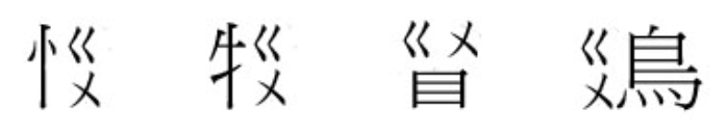
\includegraphics[width=0.8\textwidth]{./images/bopomofo_composed.png}
\caption{蔣為文以注音形聲字書寫的「愲」、「牯」、「瞽」、「鵠」}
\end{figure}



他們的方案是在漢字的基礎上發展出來走得最遠的可能。但沒有可能的——字符太多了。字符這麼多,不是沒有辦法解決,但解決的手法是社會性而不是文字層面上解決,亦即強推強教,並防止外來語文的影響。但此舉在當今如此全球化的世代是沒有可能的——除非你願意犧牲經濟利益,閉關鎖國。雲南規範彝文有字2608個,其中表意字2258個,借詞表音字共350個。雲南民族出版社1994年出版了《雲南規範彝文漢文字詞對照》。但這種文字目前沒有廣泛通行。這個方案,粵語是行不通的。此等前車不可鑑。

 \chapter{全拼音化,摒棄漢字?}

我們上文道出了漢字的問題,整個漢字體系的附帶惡性影響,本字考的限制和帶來的幫倒忙,我們可能會感覺,為何不多快好省快刀斬亂麻,狠心放棄漢字走粵語拼音化的路線?既然漢字這麼多根本性無可撇除的問題,那難道粵語的字書語文化工程就需要走全拼音話的道路了嗎?

先處理一下語義的問題。在下文,凡曰「摒棄漢字」,其所指乃「全盤摒棄漢字」,也就是「完全廢除漢字作為書寫方法」,即「改用拼音文字」的意思。同樣「改用拼音文字」亦是全盤的,沒有部分。當然,為了討論,茲假設了出了漢字這個象形象意文字和拼音文字之外,沒有第三種的文字系統,也假定了兩者本質上是互斥的。

我的結論是粵語全拼音化,是不可行的——此論至少在我們的時代,還有我們可預見的未來而言,都是理應為真的。我在此先把後話說在前頭,把我的結論先說出來吧:粵語的字書化,不可能完全依賴漢字,也不走全拼音化,也不能全盤放棄漢字。粵語的未來,在於某種漢拼混用的系統。那當然,一下子走拼音化的不可能很大程度上源自拼音化的「一下子」。如果拼音化的過程是循序漸進,幾乎無痛的,那可能性就必然提高。那問題就不再是我們能不能今天就開始走拼音化的路線,而那身處於遙遠未來完全拼音化的粵語是否一個可欲,一個我們接受的未來。我認為,在至少五百年的將來,漢拼混用的粵語都比任何一個全拼音的粵語——而在五百年之後,走全拼音路線的代價就會因為我們已經漢拼混用而大大下降。但同時間,走全拼音路的利益也必通通溝淡。現在,全拼音化既不可行實際,效益也成疑。但在這個已漢拼混用良久的世界,雖然全拼音化變得可行實際,效益不再成疑,但效益於其世界是會看得出不夠,使全拼音化不划算。也就是說,今生今世,棄漢取拼沒有辦法,也沒有肯定利益;而他生他世,棄漢取拼有了辦法,但卻肯定沒有太多利益。

\section{今生今世全拼音不可行,效益不良}

為何今生今世全面走拼音化的道路可曰之為死路一條?當中的原因很多跟為何全盤摒棄漢字不可行是一樣的。用全拼音方案,亦即全面放棄漢字,是會釀成龐大的語文混亂的。這一點我在討論為何不能摒棄漢字的一章中有詳細的討論。

其中一樣獨於摒棄漢字與否,為何全拼音化有可行性問題的原因,自於走拼音化路線的很容易遇上的問題。注意:我是說這個問題很容易遇上,甚至無可避免,不是說這個問題本質上和理則上必定會從粵語拼音化中衍生。

一個文字系統,要兼顧至少兩樣互斥的範疇:音、義。漢字就是只顧義,不標音,繼而讓音走一種放任主義的文字。但完全準確標音的系統,不代表他可以有效地表義。如果一個系統完美地標音,非常可能意味著其表義能力則有所犧牲。西方語文也是有表義性的——語素的串法,就算在不同的詞語中讀法不一,很多時候還是恆守一致的。這樣,就有意義的連貫性。亦因此,用國際音標(International Phonetic Alphabet)來書寫任何一種語言,都是可笑地不切實際,白癡非常。拼音方案所關注應付的問題,跟文字所關注應付的問題,也許重疊,但非一樣。故此,拼音方案,是不能就手拿來當作文字方案的。

其實,這個理由只不過是一個非常簡單、老生常談的論點。拼音之後「星期一」跟「星期日」難以分辨,誰都看得見。但是,〈施氏食獅史〉〈獅食豕史〉〈季姬擊雞記〉等同音文章,只證明了純拼音方案不行,但證明不了以拼音主導的書寫方法行不通。如果走拼音方案,可行方案淡然不是純拼音,而是某宗的意義拼音合一的書寫方式——泰西語文全如此。但要這樣做,就要進行極其龐大的語法整理工程,此見下。

然而,如果粵語全走拼化路線,其書寫方案幾乎必然是會建基於我們現有的粵語拼音方案,如粵拼等。而這些拼音方案,如果直接拿來即用,不經過適當的字符和書寫改造,就會不能擔任文字的責任,最後改革失敗。

通常,拼音方案不能完全承擔文字的責任,是因為拼音方案側重於標音的準確而忽略了表義的準確,而要提升表義的準確、方便、可用性,就必須犧牲某些的標音準確性,透過表音體系中出現一些約俗所容許的例外,繼而從表音和表義兩者取得平衡。而平衡的點在於何處,幾乎完全取決於其語文群體的約俗強度和習慣。英文就是一個表音非常混亂,表義頗強的西方語文。但粵語要走到這個地步,要有這個把表音和表義平衡的拼寫系統,是非常困難的——因為這個平衡是無法透過人工手段達到的。人工手段和人為設計只能輔佐,運作上很難想像如何可以整理整個龐大的語文系統中的所有。況且,這樣的設計基本上沒有可能為群眾所理解、學會、接受。這一種的平衡,必須透過有機的歷史性約定俗成機理才能達到,而這個過程是需要時間的,可能非常漫長。越南文和希伯來文,是少數成功的例子。粵語能否走上全拼音化的路線,能否仿越南文和希伯來文的發展足跡,非常成疑。

\section{拼音化需進行龐大的語法工程,民眾語感要翻天覆地}

要討論這一點,幾乎無法不緩引我就乎Narihato Ohfu成鳩王鈇發明 的吳語小字的討論(請見吳語小字),但為了斯文的完整性,我不應在此緩引。儘管如此,我會討論一下拼音化的語法工程。

其實無論我們如何改革粵文,你一日想粵語要存取到高階思哲,語法整理工程就是避無可避。但有些語文的改革卻可以延遲斯等工程,或在不完成此等語法工程就開始文字變革工程。而走拼音化卻不立即進行語法整理工程,必死無疑——為什麼?

最簡單的原因就是當我們要走拼音路線,我們就要立刻決定拼寫的分界在哪裡——我們不可能一句話一寫到尾不停頓吧,如果要停頓,就要有空格、標點符號的標誌。而分界的最簡單且最簡單單位就是詞 word。也就是說,要在一個語言中,界定一個word的定義或模樣。這個聽起來很簡單,但其實是非常非常龐大的問題。也許我們也會覺得,這個這麼基本的語法問題,語法學家理應早已處理完了吧?不然矣。所謂的粵語語法學,其實只不過是把「漢語語法學」照辦煮碗的語法整理工程而已。問題在於,所謂的「漢語語法學」,其實根本亂七八糟,到此為止也無法自恰。為什麼會這樣呢?歷事原因很多,譬如「語法學」這個東西根本就是一個只有一百年的西學中用東西,而由於他來自西方,他理論的構建是完全出自於西方語文習慣和假設的,並完全沒有照顧或考慮過「中文」和「漢(系)語」之間的那種奇怪、完全不存在於泰西語文的言文關係。由於沒有經過(或曰尚沒有)適當的本土化,所謂的漢語語法學其實是千瘡百孔的——這一點並不難發現,就連中學生也能感受到。正正因爲此等不能自洽的問題,語法學學界才會有什麼「實詞虛詞之外還有半實半虛詞」此等嚴重冒犯奧卡姆剃刀的論說。加上政治的要求和威逼,中文用家的思哲不誠實、理則崩潰、文字慰瀆,很多的語法學術都變得古靈精怪,學術討論增添了不少垃圾污染,所以才會有「粵語是漢語方言」這樣無聊絕頂的開眼謊言。為了跳出西方框架,徐通鏘提出的「字本位」語言理論 ,但又未見其發展成熟。 而徐通鏘的「字本位」理論,就是相對於西方的「詞本位」理論。

我們不難看見為何漢字是與「字本位」相容而拼音文字是與「詞本位」相容,因為他們的書寫系統就是分別要各自呈現「字」和「詞」。漢字語文自古以來就沒有「詞」的概念,也不在其語文呈現這個東西;但拼音文字,就是透過空格來毫不含糊地呈現「詞」的存在。漢字語文是沒有空格的,就連標點符號直接到二十世紀才出現。就連現在的漢字語文,仍然沒有很清楚不含糊地表示詞的分界。故此,如果我們如果要改用全拼音,我們就得完全整理語法,並且把這個語法直覺注入到民眾當中,還要讓他們熟悉這個直覺到可以用這個直覺書寫——這是非常困難的。而這個整理語法,首當其衝的就是界定詞的分界,讓我們像韓文或普通話拼音,界定詞的開端末端。但這個不是語法工程的全部,只不過是開始而已,而且是最痛苦且得益最小的工程階段。真正能讓我們存取到高階思維的,是語法部件的分類,及其語義蘊含的釐清。而這個,是必須做的,但顯然,把這個跟文字改革工程綑綁在一起,就會使文字改革工程要等。粵語等不了。

這個就是為什麼語法整理工程無論是否走拼音化,都必須進行的原因——因為我們要奪得使用高階語思領域的能力。

為什麼高階語思跟語法有密不可分的關係呢?因為「語法是一套思維體系」。這句話
Narihato Ohfu成鳩王鈇也經常說,但我認為很多人都未必明白這句話是什麼意思,也見不到例子。我覺得他這句話有點問題,就是忽略了Semantics (語義)跟語法在傳遞意思的同樣作用。泰西是語法、語義兼用且兼兼發達的,但「中文」的以語法來傳達語義的途徑,卻非常落後。試譯「What would have been wasn’t what had been, and certainly not what is」為中文。 透過屈折來傳達的「What would have been」的 counterfactual 在中文必須透過語義分析才能道出,但英文是可不語義分析也容用家說此話的——用家不懂語法背後潛在的語義,但透過語法分別仍能辨別出此語不同那語。而潛在於counterfactual語義當中的「物」就是「possible world」。這個就是英文裡頭的一個兆物觀的東西。但這個「possible world」在中文的兆物觀當中是不存在。那些以中文討論模態理則的人搬字過紙把「possible world」強行拉到中文裏,幾乎必定會枯死無果。

成鳩王鈇認為,吳語如果要奪得高階語思能力,就必須透過語法整理工程來讓文字呈現這個因漢字而被逼匿藏的屈折性。這個是非常可理的,但為什麼我認為粵語不應也不可以走這條路呢 ——或至少這階段不可以走?因為我們粵語跟吳語面對的遊戲局面有點不一樣。吳語是從零開始,一片光鮮,但粵語已經有很多的包袱和成品。我們要走成鳩王鈇的語法兼文字整理工程不是造車開車,而是砸車,然後造車,再開車。而砸車,必定很多反對阻礙重重,且並非單純來自學者,而是來自群眾。反而,吳語區的群眾語言觸感近乎零,沒有文字習慣,白紙一張,你專制指定他們如何如何反倒容易——但是在粵語這樣做就是與民作對。如果這樣,倒不如把車邊開邊改裝好過。

\section{粵字改革不能摒棄漢字}

記得有一次,好像是在中環的「荷蘭正」酒吧,有一位名為馬留先生的朋友忽然評論我當時才剛剛開始斟酌的粵語字書化、語文化問題的思考,說:「我非常支持你的工作,粵語盡快拉丁拼音化就越好!」我當時沒有回應,但實乃回應不過來,因為他的一言半語,激發了我的思緒。我的第一個感覺就是詫異,因為印象中馬留先生中文是非常不錯的,也是努力捍衛繁體字,和香港的那種特有和文、白、粵為一體的「港式中文」的文化人。一般這等人都是本字考派別的,要不然就是反對粵語白話文發展,部分甚至認為新文化運動是錯誤,覺得應當恢復文言文。我第二個詫異的原因,在於為何他似乎不太在乎或不太在意粵語語文廢除漢字或摒棄漢字的文化和經濟代價——他是一個聰明人,絕對沒有可能不知道,故此他這樣取態必定是源於他衡量過後,私理斷定還是廢漢字來得划算。亦因為他的此一語,強化了我當時對本字考可行性的懷疑。我最後的結論是否定他的建議的——粵語的字書化和語文化工程是不能摒棄漢字的——但他一語背後所包涵的可能思想卻激發了我異常的深思。

先簡單討論一下這個「不能摒棄漢字」中的「不能」的語義。 茲「不能」並非形上的「不能」——這裡不是說「粵文發展本質上沒有摒棄漢字的形上可能」。如果粵文發展本質上沒有摒棄漢字的形上可能,粵語摒棄漢字就會是一個等同要創造一個有四條邊的三角形一樣的舉措。但顯然,粵語摒棄漢字不同創造一個四邊三角形。粵語摒棄漢字來字書化,是形上上、原則上,乃至廣義的原則上所可能的。越南語完全拉丁化就是活生生的例子。粵拼的發明,乃至2019年8月份時曾滿城討論更使用風靡一時的「火星文」,均暗示著粵文完全拉丁化的可能未來。粵拼暗示粵語可以以科學拼音化的模式來字書化,而「火星文」的出現更證明著粵語可以走英文那種不問拼音是否科學有條理的路線。

故此,我說粵語「不能摒棄漢字」,意思是指如果粵語摒棄漢字,效益不斐不划算。效益乃利益(優處)減去代價(弊處),而我認為粵語放棄漢字的效益,利益雖有,但代價非常高昂。這未曾以為使用漢字就只有益處沒有壞處,使用拼音就百利而無一弊。粵語字書化的工程,使用漢字和使用拼音,均有其體似星座的利弊集。我們要做的,就是找到一個可以把效益最大化的方案,而摒棄漢字,不是該方案。

那當然,我這裡是假定了考慮的集合只包括「漢字」和「拼音」兩者。

之前的數個章節,我已經討論過了使用漢字會帶來怎樣的長遠惡果,也就是使用漢字的代價。在此,我會說明一下摒棄漢字的代價——亦即使用漢字的利益——繼而說明粵文為何不能摒棄漢字。

\section{漢字與粵語的千絲萬縷關係}

使用漢字來語文化自己的口語,長年累月之下,漢字的特性和運作理則是會對其語言產生改造效應的。這個改造的效應,在一個語言的所有層面上都有其運作,包括音系、表意理則、思維模式,等等。這一點沒有什麼好爭議——亦非漢字語文所獨有,西方的拼音符號亦有同樣對用其者之語的相對影響。我們舉幾個漢字如何影響其使用語的例子:上古漢語是多音節的,音系非常複雜。但由於漢字是方塊形狀的,一塊一塊、一個一個,這個在書面上的存在模式主宰了其美感的理則,故而主宰了上古漢語的詩歌乃至整個高階語文的發展理則。其理則演化成為了發展機理,最終導致漢字語素乃至詞語單音節化,複音節語消亡。 日語開初借用漢字來書寫,亦出現了單音節發展的情況。韓、越亦然。

粵語比日韓越三者為漢字所薰陶早得多,故此漢字在粵語所施展了語言影響也比日韓越所感受到的厲害。此議無好置疑——是正正此因,粵語才有自信挑戰普通話作為「中文」甚至「雅言」的身分和地位。

既然漢字在粵語身上有這麼深和不簡單的烙印,要摒棄漢字的話,其影響一定不斐。要知道,漢字的運作理則是深深鑽入到粵語的骨髓中。我們閱讀、書寫、語思,都冥冥受到漢字所影響。姑勿論茲茲影響是好是壞——雖本人認為整體而言,影響壞勝於好——由於影響這麼深,貿然廢除漢字,粵語的運作會被粗暴打亂。這一種的打亂,是可以感受到的。當我們讀一篇全粵拼文章,讀得五不像好像文盲,就是我們已經習慣了,已經用上手的語文理則,無法霎時應付新理則而兵荒馬亂之況——亦乃我們突然放棄漢字所必然經歷的過程。同樣,我們要用粵拼書寫,遲遲提不起手,無法流暢,亦同理。

但當然,這個理則的對接不符,接觸點不良,不是本質性的,而是慣性的。既然是慣性,就可以改,而改得夠慢,就可以幾乎無痛。最重要的是,這個粵語理則因使用新文字系統而被打亂的現象,是一個存在於人語思空間和語思機械的,而不是本自於粵語本身。我們說「貿然廢除漢字,粵語的運作會被粗暴打亂」的意思不可能是廢除漢字,粵語本質的運作會墮亂或崩潰,而是指身處於廢除漢字一代的粵語人,他們使用粵語語文的理則要大規模逆轉,而次逆轉大規模而痛得很。這個「痛」可能於聽講讀寫四範疇的能力下降呈現之。你想想,如果粵語廢除了漢字,整個社會全改用粵拼,即時過渡期足夠漫長,你自己作為一個個人的聽講讀寫的能力也很可能會大規模退化——嚴重則等同製造了大量的文盲。可知道,日韓越三國的廢除漢字轉用假名、諺文、拉丁文之所以成功,很大程度上是因為當時國裡的文盲數量非常多,不懂漢字根本就是主流,故此廢漢改用才能產生去文盲的效果,而不是變相製造文盲。中國大陸推行簡體字也是在文盲多的情況下成功的,而當文盲數量下降,民眾的語文慣性提高,要大規模整頓文字系統的成本就會遞增——二簡字失敗其中的一個原因,就是因為新的二簡字的運作理則跟已經習慣了一簡字的民眾用字理則相距太遠,釀成混亂,最終失敗。但「貿然廢除漢字,粵語的運作會被粗暴打亂」並非囿於語言心理的層面上。廢除漢字之所以很可能會導致粵語的運作被粗暴打亂,是因為廢除漢字意味著粵語人理解、使用粵語語素的方法要完全改變。而正所謂「上屋搬下屋,唔見一籮穀」,這個改變——因乎其過程的粗暴——可能對永久導致粵語永久喪失某些語素。由於使用語言的理則變天,人的不習慣和不純熟會使所有人為求不犯錯不出醜而只使用最簡單和最不會犯錯的語言部件。這個很正常,香港人說普通話或英文不會特別詞語豐富,中國各省人士說普通話盡求使用通俗詞而少用高階詞,句式趨向簡單,亦說於此。為何文字上的改革會導致口頭上的語素和語言能力產生變化?這個上文實已略道:一、漢字的運作理則崁入了粵語的運作之中,廢除了漢字,粵語的口語運作就變成了空中樓閣;二、我們粵語語思對語素的處理某程度上(當然不是完全)依賴漢字——當我們聽到一個語素時,要解義就往往要尋找其漢字對應並以其漢字來解義——但這個不是絕對也不是全部的語素的解義方法。尤其穩定穩陣的粵語語素,是用不著此法的。但如果是比較偏門,用次較少,在語群中已經陌生的語素,該等語素依靠語群本然獨立於文字的自然語感來義解的能力已經退化,在沒有漢字作為承托的情況下,他們消亡的機會是很大的——問你意思又不知道,又沒有漢字讓我們猜度或推敲其意思,那結論就是我們不知道該語素的意思和用法——死亡就是結果。全盤廢除漢字一併改用拼音的效果有二:一、本來有漢字作為意義承托的語素都失去了承托,一定要依靠新以拼音呈現的語義單位來承托,要不然就只能依靠自然語感。二、由於用家一定會有一段的時間不習慣使用新的拼音來承托其語義的考究,其不純熟和不習慣的結果就是語義的在所有可用方法之範式,包括自然語感,都考究不成功。還有,我們只談到語素的掉失,還未談到句式簡化所帶來的理思自閹和語法殘化。合上二論,整體效果就是在這個大逆轉中,極其優量都勢必造成大量的語素被忘記、摒棄、失佚,導致整個粵語語文系統的短暫退化。而粵語能否從此退化中重振起來,沒有擔保。亦即,這個殘化,有可能不是短暫,而是永久。
\section{文化衝擊,文化斷層——精神真空}

上述語文使用習慣逆轉所產生的問題的類比和規模延伸,就是文化上的衝擊和斷層。衝擊就是新東西的湧入,斷層就是舊東西再無可存取。

這個理由其實很老土,邏輯也很簡陋,沒有什麼營養——這一種的詏論經常於繁簡字的爭論,也出現於越南和韓國摒棄漢字的批評中。為什麼說其詏論老土、邏輯簡陋、缺乏營養?因為此等「文化斷層」的詏論所訴諸的,是某種的「傳統至上主義」。他們認為文化傳統是神聖至上,不可侵犯也不可更易摒棄,但為何文化有這樣神聖的地位,他們是不會也無法說明的。在其論中,文化的神聖性總之就是這樣,不用解釋。

我們可以注意到,按照茲等邏輯,任何更易文化的舉措,於其範式中都是不可為的——無顧乎更易的效益是什麼。此等教條主義者於漢字使用群中數量特別多。如果西方沒有發明到電腦,而如果漢字的運作效率和精準度是不足以讓華夏文明發明到電腦的話,此等傳統至上主義的教條人士是會寧願不發明電腦也要保住漢字。他們之所以這樣,有這樣死板和頑固的文化性格,是因為「漢字神話」所發揮的精神性俘虜了她們的心智,使他們不能拜託漢字、膜拜膜拜。漢字變成了他們心目中的一個義值,一個理則上無可挑戰的本自好。最重要的是,通常渲染著此等意見的人士,他們自己本身因為他們已經精通了漢字語文,在「漢字神話」的精神世界及其催生的文化和政治秩序中,是會按乎「漢字神話」的理則被判為文化和政治菁英的。也就是說,他們在他們提倡的秩序中是既得利益者。他們這樣的提倡,完全是自私自利的。

顯然,用這樣的思考模式來衡量我們的語文的未來發展是白痴。

儘管如此,粵語全盤摒棄漢字所釀成的文化衝擊和斷層卻是鑿鑿有據的,不是危言聳聽,亦非虛謬。更重要的是,廢除漢字是幾乎肯定會造成文化和社會價值的崩潰和真空。這個是開了一個潘朵拉的盒子——粵語摒棄漢字很可能會開發出一個充滿危機的不可知。

漢字中所散發的價值觀,是具有精神性。漢字使人著迷。使若非焉則 聰明思敏的人理思崩壞,源自此精神性。這個精神性存在於使用漢字的人心目中。那當然可以有強弱有別,因人而異,但不可能不存在。也就是說,大凡某人使用漢字,該人的心靈中就必定有其精神,該人的理思議會,就必定有代表者漢字精神的價值的代議士在諫議東東西西。而這個精神性,使人的內心的恐懼和懷疑,透過從外在世界的特徵和狀態,抽取能力給予內在的心靈,提供精神上的支持。也就說,使用漢字的人,是會構成一種從外在文化政治環境提煉精神能力的生活習慣的。如果沒有了漢字,他們的命運就是一個漫死過程,而該存於心中的精神性則漸歷久無新貨供給而像餓死的癌細胞一樣,萎縮而末。這個是一個精神痛苦的過程,故此他們會很驚慌地想要解決這個問題。一般而言,解決的方法就是尋找新的價值體系,放到自己的心智當中扮演「漢字神話」的精神角色。夫問誰能代替爾地位?無人也。故此,人是會瘋狂嘗試重立漢字,以及其精神的極致。這個現象,一般是不會產生任何新的思哲產品的,反而是會產生各式各樣更加鞏固「漢字神話」的精神產品——而唯一一次例外,就是清末民初的「寒夏思潮」。但注意「寒夏思潮」的最終目的,也是漢字神話的精神性的政治秩序的救亡、振興,達華。更重要的是,在這種價值體系在現實世界崩潰,導致個人心理兵荒馬亂的情況下,人是很容易分泌出很多古靈精怪的危險思想的。

以最好假況而臆論之,所有生產和分泌出來的思想都是良性和能讓我們遠離墮回到漩渦當中的話,這個可能性仍低得很——繼而使廢除漢字以得粵語的勝利這盤賬不划算。為什麼這個可能性很低?因為歷史上從來沒有出現過——就連「寒夏思潮」這個華夏終極的思哲大爆發也只有小貓三四隻。老毛說過的做過的湖南,最終也成為二十七的自古以來。所以絕大部分在這個因廢除漢字而在粵語群爆發的群龍無首兵荒馬亂各顧各的思哲亂世,就算沒有淪落至狗咬狗骨的自然狀態,幸好產出百花齊放的境況也不必永遠,反而很可能是我花開後百花殺。放棄漢字所產生的價值崩潰情況,風險高,不確定性也高。

我不是說這個價值觀,我們現時的「漢字神話」有什麼值得保留的價值——保留的價值是有的,但是是保留於博物館的價值。我誠認為這個現時的價值秩序和精神必須滅亡,但這個滅亡必須小心處理,否則我們不但可能死亡慘重,甚至可能永遠錯失一時勇舉截阻萬世苦的良機。 

\section{資產喪盡,文化破產,軟實力歸零}

此外,比較直接的就是文化經濟實力的考慮。這個其實是個很明顯的考慮,但為釐清放棄漢字而意味我們終必需連此一同放棄的代價之龐大,還是要不厭其煩闡釋清楚。

粵語的文化資產,是整個漢字語文家庭中,繼以普通話為首的官話之後,最為豐富有米的成員。其文化資產的質素,甚至論至超越普通話的也不為過。雖然粵語的文學非常薄弱,根本沒有所謂的粵文文學,但粵語在白言文的影響還是不少的。粵語的文化資產,大概可以分為以下範疇:古典中國文化資產、當代中國文化資產、香港粵語文化資產,和傳統廣東粵語文化資產。

古典中國文化資產:即傳統古典中國的所有思哲和文學產品,上至先秦兩漢的春秋諸子,下至清末民初的所有思想、潛哲學、待發體系、醫學、政治、科學、歷史、文學、文化、衣食住行、傳統、迷信,等。儘管當中不少內容是完全垃圾和荼毒人心的劇毒,好貨還是有的——而且闡發的潛能不薄。粵語應當注意的是:一、粵語是繼官話之後最能夠存取中國文明的漢系語言,亦即南方諸漢語存取古典中國文化能力為首的語言。單單「入聲」一者就勝官話胡同街萬條;閩南語欲有粵語之位,遺憾下世仍算早;吳語則已自刎,無庸議。二、適當地存取這個文化寶庫,小心地闡發其內容,是可以讓我們獲得驚天地泣鬼神的思哲效益,然後讓我們得到難以思量的經濟利益。除了是不通《三國》無法造「三國無雙」和「三國殺」等能產生文化軟實力和帶來經濟收入的產品之外,我們錯過的,是哲學上稱霸的機會。當然,這個我們要存取和闡發讓我們發達的,不是那些食古不化的經文,亦非那些自古以來一直未蒙重視,長久忽視甚至鄙待的思哲體系(如墨家),而是那些透過激烈批評、批鬥、甚至煎皮拆骨之後而得出的精華。中國古典文化應有、應得的、熱切期待的,是巨星殞落式的思哲大爆發——一場屬於自己華夏文明的啓蒙運動。啟蒙運動,不單純是批鬥,而是以子之矛攻子之盾,兒子透過父親教導的玄理真義來打死父親,是自己使用自己的理則棒打自己的理則的自虐得道過程。如果無法存取這個古典文化的內容,就無法進行這個的啓蒙——而茲有三點壞處:一、亦首要者,粵語需要這個啟蒙,才能存活,否則必死無疑,這個是政治現實;二、粵語是最能夠且最有潛能,其民眾最願意進行和牽頭這個啟蒙運動的語言。我們不做,華夏沒有人做,有也必定做得不夠我們好,泰西就更加不用想——他們根本不知道華夏是什麼;三、如果我們不做,就等同白白奉送了一個文化神力大增的機會,好牌人家贏,輸牌自家賠。

當代中國文化資產:這個指清末民初到現在整個大中華的思哲產品——主要以白言文為主。不要輕視這一個資產的潛能。如果古典中國文化資產是一個金礦,當代中國文化就是一個油田。這個油田包括嚴復的《群集權界論》,金岳霖的《論道》,毛澤東的《矛盾論》,張愛玲的《傾城之戀》,金觀濤的《興盛與危機》。這個是一個論高白馬,道超青牛的時代。寒夏民國的潛能,是遠超於春秋戰國的——也實在實用得多——理則學、語言學、政治學、倫理學、經濟學、建築學、數學、科學、文學、音樂、藝術、美學,全部都是實學,遍地黃金寶玉,而且通通有待闡發,潛能驚人。可知道,要存取當代中國文化資產,某程度對古典中國文化資產的把握是入行的前提。沒有《道德經》,金岳霖的《論道》價值不降閱讀也難度倍增。

香港粵語文化資產:香港的粵語文化資產當中有不少是食兩家茶飯的,既是當代中國文化資產,也是香港的粵語文化資產,譬如張五常的《新賣桔者言》、金庸的武俠小說,衛斯理的科幻小說,饒宗頤、牟宗三等大師的著作等。他們使用生為官話白話文,但在香港已演變為有香港粵語味道的白言文,使粵語擁有了一種屬於自己的普天通行語。《明報》《大公報》《文匯報》的語文,一般都是使用這種白言文的,故此都是香港粵語文化資產。當然,這個範疇也包括了各種純粵語的文化產品,如《蘋果日報》的粵文文章,高登連登上的各種潮文,香港粵語的各種俚語,香港粵語的電影、電視劇、流行曲、音樂、藝術家、歌唱家、填詞人——以及他們的剎人的風骨和可惡的人格破產,通通都屬於這個範疇當中。這個範疇,電影電視包含了李小龍、張國榮、梅豔芳、周星馳、梁朝偉、劉德華、張曼玉、陳法拉、陳奕迅、黃秋生、杜汶澤、黃子華、MLA。

傳統廣東粵語文化資產:這個明顯就必定跟香港粵語文化資產重疊甚多,但當注意絕大部分的廣東粵語文化是香港的粵語文化資產,很多的香港粵語文化資產卻不是廣東的粵語文化資產。有些傳統廣東粵語文化,是香港粵語文化所共有的,因為他們是整個粵語文化的共同資產,如飲茶文化、粵菜、粵劇的學問,香港和兩廣的粵語文化研究和產品等。

這些文化資產,全部都是建基於漢字的基礎上,要透過漢字來存取的,而茲茲就是粵語的所有身家性命財產。如果摒棄了漢字,所有的這些文化資產都勢必封印於歷史和博物館當中,不能為民眾所存取,其連帶的文化軟實力都必然消散。沒有文化軟實力的語文,就必定膳不安寢不妥,朝憂暮亡,夜慮旦滅。摒棄漢字,粵語的文化資產撞情況不會是十九世紀初的日語,二十世界末的韓語,連越南也不是——情況將會是差過曾死要復活的希伯來語。這個是完全的文化真空,是徹底的文化「一鋪清袋」。

\section{漢字情意結使摒棄漢字推行成本極高}

上文提到漢字中的「漢字神話」以及漢字的精神性如何左右一個人的精神狀態。這個精神狀態所散溢的情瀰,薰陶著漢字用家的文化忠誠和政治志向。茲茲現象當然牽涉到我們摒棄漢字的利弊考慮,但其實摒棄漢字最直接限制,就是要這樣做的成本龐大,失敗率極高。

「漢字神話」為人提供精神上的輔佐,人渴求這種精神上的慰籍,故此自自然視漢字為美,對漢字產生情意結。而要破這個情意結,是要有成本的。這個不單單是實質經濟上要重寫書,把公共場所中所有漢字都換掉,重新設計所有教育系統,重調整個社會的語言運作茲等舉措——就算你這些什麼都不做,廢除漢字就等同要滅有漢字情意結的人的精神世界。既然如此,他們就必定會反抗。由於我們的舉措如此激進,他們的反抗也必相應激進,故而導致成本進一步攀升。最重要的是,摒棄漢字此舉非常「撲面而來」,故此正力越大則抗力越大。

漢字情意結如何導致廢除漢字的成本提高是一個值得闡述的問題,當中「漢字神話」的部分運作機理應當加以闡明釐清。「漢字神話」導致人不能拋棄漢字的最重要原因無非其精神慰籍,而這個精神性的來源,是跟美感息息相關的。「美」乃漢字何以有神話的原因。漢字的成員字符象形象意兆物觀,存在於其字的表面、裡面、和後面。而這個象形象意兆物觀,因乎其象形象意於字中,不像西方拼音文字存在於口語中,而是在漢字的書面呈現上,像礁石般按時按候於波浪的波峰與波谷之間披露頭角——剎我們一個措手不及。這個美感因為可享,故此享用嚮往的人歷久就必然發展出一種的品味敏感度。而當他們面對新的美感體系,最追求的,就是漢字美感可以給予他們的精神——而美感上的享受,是該精神的先行前提。也就是說,如果新的文字系統,沒辦法(而我們都可以頗為肯定,任何的新文字系統,都必定不能)像漢字抒發同樣同質的美感,漢字神話已經中毒已久的則會發狂,毒情輕者則會間接排斥、否議、罷用。

面對這樣,一係就落重成本大力強推,一係就放任不理透過漫長的改造過程,消磨和消除該漢字神話的依賴性——猶如戒毒。兩者都成本不菲,但前者遠比後者高,成功率也必後者低。

\section{摒棄漢字不可為,粵語字書化必定要有漢字才能成功}

任何全面摒棄漢字的粵語書寫方案,可行性成疑,成本不菲。茲意味粵語的字書化方案和語文化工程,都無法擺脫漢字。但這個不意味一定要完全使用漢字,也不意味拼音文字不用考慮。

可知道,利弊有份強弱厚薄。使用漢字書寫粵語,也是有成本的。而其利弊分佈也不是一成不變,而是會按時空和歷史環境的演變而更易的。粵語之所以在可預示的將來都不能摒棄漢字,是因乎於我們今天身處於的宇宙組態。若非世當如斯,我們可以從中選擇的可能性集將應當頗為不同——而於其可能性集中,摒棄漢字不是一個不可能而是一個可取之道,絕對是一個可能。而這個可能性集或者不是我們今天擁有的可能性集,但可能會是我們未來所可以面對的可能性集。到其時,摒棄漢字的利弊效益組態,又可能不再與今同一。但到其時要否放棄漢字,就是一個因乎其之遙遠而近乎無關的問題了。

全拼音今世不可能,漢拼混用方為上策。
 
\chapter{坊間拼音方案的侷限}

如果粵語字書化和語文化的工程的核心方法是「漢拼混用」,那這個「拼」應當是什麼呢?我們姑且稱這個我們用來跟漢字混用書寫粵語的拼音系統為「粵拼字」。這個粵拼字系統,應該是一個怎樣的系統呢?

與其抽象地列出一個適合的粵拼字系統應有怎樣的特性,倒不如直接看看世間上萬國所用的文字方案,他們各自又怎麼樣的特性,繼而衡量優劣利弊。最好者則改動應該改動的地方就拿來即用。那當然,這個方法其實還是潛在要釐清一個適合的粵拼字系統應有怎樣的特性的問題——否則我們何以「繼而衡量優劣利弊」?但這個其實不是一個太大的方法缺憾,因為如果某個文字系統在書表粵語上存在語言上的問題,我們是可以透過改動該文字系統的使用方法,以求吻合可用的。那當然,有些文字要符合這個改動使用方法來符合某些語言的可改性有限,左改右改也可能最終失敗而回,或搞得古靈精怪無法使用。但在這些情況下,我們不用他們就是了。茲意味,某個文字系統能否完全能夠書表粵語,是一個可以以手段緩和的問題,也是一個次問題。如果文字系統甲跟文字系統乙相比,甲比乙要修改才能使用的程度為低,那選甲就是了。問題在於,如果甲、乙、丙、丁,都不用修改,或戊、己、庚、辛修改後都書表能力差不多,那如何判斷優劣?文字系統選擇的競爭是不能打和的。

\section{諸他不易,蓋事慮及,美為至}

這句裝模作樣的偽文言的意思,就是「ceteris paribus, all things considered, beauty is the final measure」。也就是說,倘若所有其他條件不變,且考慮過所有的應考慮的因素後,「美觀」是我們選擇的最終標準。  如果一個文字系統,能夠完美地把粵語字書化,但是醜極了,我們還是要把它撇除否決——或,把他改造至夠美為止。為什麼要將它否決?因為,如果不是我們把他否決,就會是民眾把他否決——斯說之於「漢字神話」。而由於我們是漢拼混用,粵拼字字符美感所要對壘的,是漢字的美感。嚴格論之,如果漢字和粵拼字的美感出現對壘的情況,這是極度不理想的。這個內部美感出現鬥爭和矛盾的文字必定會崩潰,直至兩者倖存其一。而在這個鬥爭中,勝出的幾乎必定是漢字,那我們的粵語文字改革的工程就失敗了。就算我們花盡我們所有的語言文字資源和權利去強權逼使這兩個鎖乎於戰的美感達到一個人工的太平,這個太平仍然是不能泯滅掉潛在的矛盾的,而單單這個矛盾,就足以廢掉我們嘗試透過粵語文字改革以存取到的利益,我們花到粵拼字之中的設計考慮,都必然無法施展顯效。
\section{回應阿澤}

我們下文會再深入討論不同的容選粵拼字方案有什麼的問題,但在此,我先引用一下阿澤的討論。在一篇題為〈粵文書寫方式續探〉的文章中,其中一部分討論了使用漢字以外的方案的種類及其優劣。 為何要考慮漢字以外的書寫方案?因為:
\begin{quotation}
有時,大概係寫一千字會有一次咁上下,大家會有啲講法想寫,但係又寫唔出,好多時係底層詞、擬聲詞,又或者係英文借詞。於是就有人質疑「用漢字寫粵語」呢個前設。呢一點可唔可以質疑呢?事實上鄰近有唔少地區有多於一套書寫系統:台灣有注音符號,日文有假名,韓文有諺文。粵文又得唔得呢?如果唔堅持樣樣嘢都造一隻漢字,自由度係咪更加大呢?答案肯定係「係」。

\end{quotation}

然而,使用漢字以外的書寫方案,就必然牽涉到美感的問題。就美感而論,幾乎就肯定可以馬上否決拉丁化來拼音化的可能。

\begin{quotation}
不過漢字同拉丁字母睇落好唔夾。於是又有人諗,要整得美觀,不如學東亞其他相似系統,去為粵語整一個方案。早喺民國初年就有人用注音符號去寫粵語嘅發音,其後又有好多官方或者民間嘅變體。其餘嘅方案仲有諺文書寫、假名書寫、自創文字等等方式。 

\end{quotation}

阿澤為了對比不同的粵拼字方案,寫了一段非常精簡但寶貴的分析。他把以下(以普遍香港粵語文字發展工作群所認為「約俗」的粵字寫的)句子,以不同的文字方案寫了出來,方便對比。



\begin{longtable}{|l|p{7cm}|}
\hline
\textbf{書寫方案} & \textbf{例句} \\
\hline
\jcz{}
\batang{}
粵漢字(港粵主流) & 呢度啲虢礫緙嘞嘢,你幫手keep住先,我地hea陣返黎拎。 \\
\hline
「偽正字」 & 邇度尐虢礫緙嘞野你幫手keep住先,我等迆陣返來領。 \\
\hline
漢字粵拼混用 & 呢度啲 kik1 lik1 kaak1 laak1 嘢你幫手 kip1 住先,我哋 he3 陣返嚟拎。 \\
\hline
粵語注音符號 & 呢度啲 ㄎㆶㄌㆶㄎㆶㄌㄚㆶ 嘢你幫手 ㄎㆴ 住先,我哋 ㄏㄝ 陣返嚟拎。 \\
\hline
粵語假名 & 呢度啲キックリックカックラック嘢你幫手キープ住先,我哋ヘー陣返嚟拎。 \\
\hline
粵語諺文 & 呢度啲{\koreanfont 킥릭칵락}嘢你幫手{\koreanfont 킾}住先,我哋{\koreanfont 해}陣返嚟拎。 \\
\hline
純粵拼 & ni1 dou6 di1 kik1 lik1 kaak1 laak1 je5 nei5 bong1 sau2 kip1 zyu6 sin1, ngo5 dei6 he3 zan6 faan1 lei4 ling1. \\
\hline
英串粵文(火星文) & ni dou dee kick lick lark lark yeah nei bong sau keep chu sin, ngo day hea jun farn lei ling. \\
\hline
\end{longtable}


觀乎茲等不同的文字體系,阿澤認為諺文其實是最好的選擇。但是仍然要面對切實的現實推行問題,終歸導致透過諺文來完全書寫粵語不太現實,極其量只可以用作為輔助系統。

如果想「工整」,用諺文一定係最好選擇。原因係韓語同粵語嘅音系有相近之處,都係 CVC 嘅構造,諺文又係方塊字,形狀都夾。但係可惜香港嘅韓文普及率極低,而外來系統夾極都有個譜,總會有嘢撞。一隻半隻字用其他系統輔助尚可,全部轉做輔助系統,並唔現實。

阿澤因乎粵語諺文的推行困難和潛在或有的匹配不符可能,認為終歸最為可行的方法仍然是「漢羅並用」。這個我不同意。我認為「漢羅並用」根本不可能是一個推行的方案——這個極其量都是暫時的坊間玩意,不能作為長遠的發展方案——我相信這一點阿澤是絕對認同的,但由於他認為至少暫時而言,可否實行(implementability)應為衡量粵語文字方案的最高準繩,故此「漢羅混用」是最沒有辦法中的辦法。我也關注實行性的問題,但阿澤跟我不同地方在於,他對「實行性」的理解是非常建基於粵語現時佔有席位的體制中,粵語有什麼的勢力去發揮推進粵語的發展——而正正由於粵語所有去發揮推進粵語的發展的勢力都非常薄弱,我們嚴重缺乏甚至沒有教育、經濟、法律、文學等範疇的主控權,粵語的勢力只有坊間語言群可以依賴。我們沒有學校去強推一個經過精密設計的粵文系統,故此只能退而求其次,而其次很遺憾「次」得很,是「漢羅並用」——那沒辦法,只好暫時如此:


\begin{quotation}
由文字發展嘅角度去睇,為粵語創造一套新表音文字必然係最「科學」嘅方法,亦都可以滿足最多嘅要求,但係發展上粵語區缺乏誘因(冇文盲,識字率極高,本身大部份字已經有得寫),亦缺乏條件(未有支持粵文書寫嘅公共行政機關,粵語學界未有共識)。而所謂「最理想嘅方法」,喺未有條件之前,最終只會係小眾嘅玩意。另外每一種創新嘅系統,都係衝擊緊用方塊字嘅系統,究竟應唔應該做?照睇大眾嘅意願係唔想,我哋嘅文字習慣未足以令我哋覺得要為咗唔夠 1\% 嘅書寫不便去到放棄漢字。現行做法係以漢字書寫為基礎,而混合式書寫,暫時就只得漢羅並用係有實行(implement)嘅可能性。

\end{quotation}

我也關注實行性的問題,但我認為,粵拼字的實行可否很大程度上取決於美感的考慮,這個是最龐大的考慮,也是最無可透過科技手段解決的問題,更是粵拼字能否不被漢字鬥死的決定性因素。沒有學校,有互聯網;沒有大公司為粵語人設計粵語輸入法或鍵盤,可以坊間研發;發明了某種的粵拼字,沒有辦法放到網上,unicode 沒有受錄,定有手法處理。而這些所有的方案,取決於有一小群但非常忠心的語言群,一個能夠建立、維持、鞏固、發揚粵拼字外圍群的核心粵群。而要建立這個核心群,你就必定先要俘虜了他們。美感,就是我們把他們從漢字的精神性解放出來的終極要求。故此,美感是衡量粵拼字方案優劣的最高準繩。

\section{平行系統美感的張力}

粵語書寫要漢拼並行,而成功與否取決於美。漢字已經有自己的美感理則,這個是既定的,是常數,無可變。可變者則乃「粵拼字」的美感。

論美感理則,有宏觀美感和圍觀美感的理則之分。這個不是一個嚴謹的分析體系,但我們要有分析體系來處理一下的問題,嚴謹精密與否的問題必須擱置一邊。宏觀美感的理則,讓我們知道漢字和拉丁字母和阿拉伯文三者,是不同的文字系統,亦乃為何我們認知漢字、日本假名、諺文、喃字、注音、方塊壯字等屬於同一類系,拉丁字母、希臘字母、西里爾字母同屬一系的理則——但至於為什麼我們能把漢字、日本假名、諺文、喃字、注音、方塊壯字在於統屬於漢字族下再而細分,是因為微觀美感。微觀美感的分別大少能夠動搖一個子字系能否被認定為自成一格的字系。粵字比吳語字更似獨立文字系統,就是因為粵字的微觀美感於白言文漢字的微觀美感的分別比吳語字與其之的分別較大。宏觀美感上有分別的二字系是會有美感上的衝突的,微觀美感上有分別的字系則衝突較少,甚至沒有衝突。

我們與漢字並行的粵切字應該與漢字有宏觀美感上的分別,還是應該有微觀美感上的分別?如果取前者,有宏觀美感上的分別,則會出現美感衝突——而於斯等情況,就會發生鬥爭。這個鬥爭是漢字必勝的,故此會導致粵拼字系統的消亡,亦即改革的失敗。但如果取後者,就得考慮小心到底微觀美感上於漢字的分別要達到那樣的程度。誠然,由於漢字神話和漢字美感的因素,「走得太遠我不喜歡」的門檻非常低,很容易就會觸動到漢字使用者的那種「亡國感」繼而產生上述提到的各種不良反射作用,所以應該至少今生今世而言,粵切字的微觀美感是不能離漢字走得太遠的。

\section{羅馬拼音}

羅馬拼音難看不堪——望文心異。任何使用羅馬字母的拼音,因乎是跟漢字宏觀美感相異的字系,故此都必定失敗,無可考慮。這包括粵拼、耶魯粵語拼、廣州拼音等。但我們不能使用它們的字符書寫,不意味我們不能使用它們的拼合系統——理論上,只要把字符都從新設計過不用拉丁字母就可以了。台灣閩南語白話字(Tâi-oân-ōe)、臺羅(Tâi-uân-uē)、客家白話字({\taigi Pha̍k-và-sṳ̀})多年勢力甚微不發的教訓,就是羅馬拼音是不會敵得過漢字的。如果要改用拉丁字母,就要把漢字一個不留殺全家,如中國蘇維埃的「拉丁化新文字」Latinxua Sin Wenz或越南的國字。


但單純把字符體系改了並不代表就可以成功——下文會再加深探其例子。

\section{注音符號——表音方塊字、注音方塊字}

台灣的注音符號,是清末民初切音字運動中眾多方案的倖存者。在台灣,已經經改造後產生了用來書寫閩南語和客家話的注音子體系。民國政府時期,國語統一籌備委員會於1932年四月初版的注音符號總表中有以注音符號為基礎修改而成的廣州閏號分表。中華人民共和國成立後,廣東省人民政府文教廳1950年代頒布了新的粵語注音方案。近年的類似系統即有陳氏粵語注音系統。 

我們在這裡不會詳列他們個個方案的細節,但這些注音符號系統,分別在於所選的符號,全部都是線性拼寫的。而入聲字的韻尾,都是小寫的。譬如,按照《1950年代廣東省人民政府文教廳粵語注音方案》, 「熱」jit6寫作為:ㄧㄊ。這個跟台灣的閩南語和客家語注音符號的拼寫方法,是一致的:拼寫是線性的,入聲小寫處理之。

\subsection{線性寫?合體寫?}

注音符號作為粵拼字的書寫系統的最大問題,在於它是線性書寫——這個問題假名也有。為什麼這個是一個問題?因為以香港為主的粵語使用群的閱讀習慣是方塊性的。這個閱讀模式的轉變有別於中英夾雜的閱讀模式。同時間,這個也跟漢字為體而生成的方塊性美感衝突。

顯然,這個線性文字與方塊文字的美感衝突不是無可救藥的。應該是這樣說,如果粵拼字取線性為書寫模式,這個必然會跟漢字的方塊美感衝突,而這個衝突,必須要靠其他的手段來鎮壓,直至到該漢拼混用的粵文系統的用家群習慣了,建立到足夠穩陣的約俗和慣性,繼而使其美感衝突化之為自己的美感理則的一部分——日語就是經歷了這個的運作。香港粵文中的中英夾雜也可以相對穩定也是這個道理。但一個透過注音符號來建立的粵拼字完全沒有這樣的約俗穩定性,故此根本很難勝出。要提高注音符號能勝任粵拼字的可能,應該要走合體寫方向。但其實這個也幫助不了太多,因為就算是這樣,這樣成之我們姑且稱之為「注音合字」的粵拼字仍然實在太醜了。

\subsection{注音合字、表音方塊字,通通太醜怪}

網上有一個名為「表音方塊字網——中國表音文字研究交流平台」的網站。該網站主張漢語拼音字化,部分人士建議把注音符號合併起來成為方塊字。但我結論的撮要,就是表音方塊字的缺憾與注音合字的一樣:太醜。在該網站上,亦有部分研究拼音字化的發燒友訂立不同的「注音合字」。 我們在此看看圖片:

\begin{figure}[h]
\centering
% 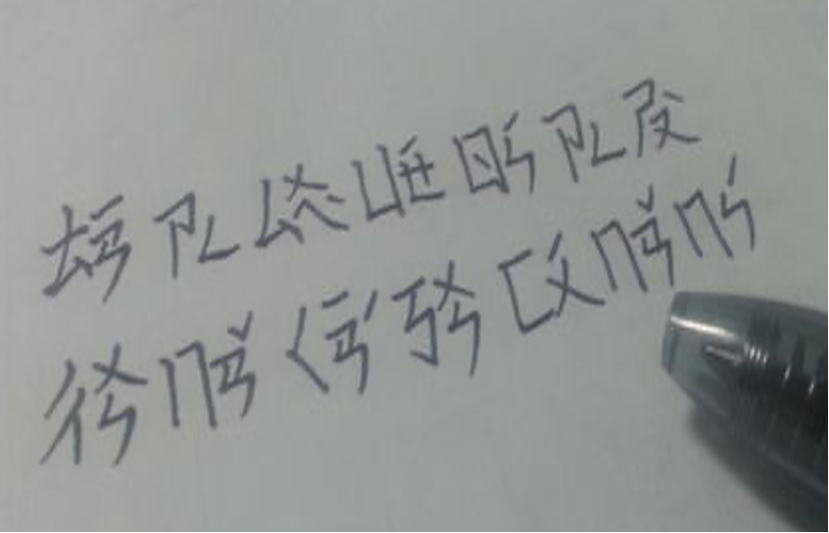
\includegraphics[width=0.8\textwidth]{./images/zhuyin_composed_1.png}
\caption{注音方塊字評語:「用原本漢字組合的方式拼不就好了。」}
\end{figure}

\begin{figure}[h]
\centering
% \includegraphics[width=0.8\textwidth]{./images/zhuyin_composed_2.png}
\caption{設計者:道皃特點:在註音符號的基礎上,對少數字母進行了修改。字形結構有上下、左右結構。}
\label{fig:zhuyin_composed_2}
\end{figure}

\begin{figure}[h]
\centering
% \includegraphics[width=0.8\textwidth]{./images/zhuyin_composed_3.png}
\caption{經過修改的注音符號}
\end{figure}


\begin{figure}[h]
\centering
% 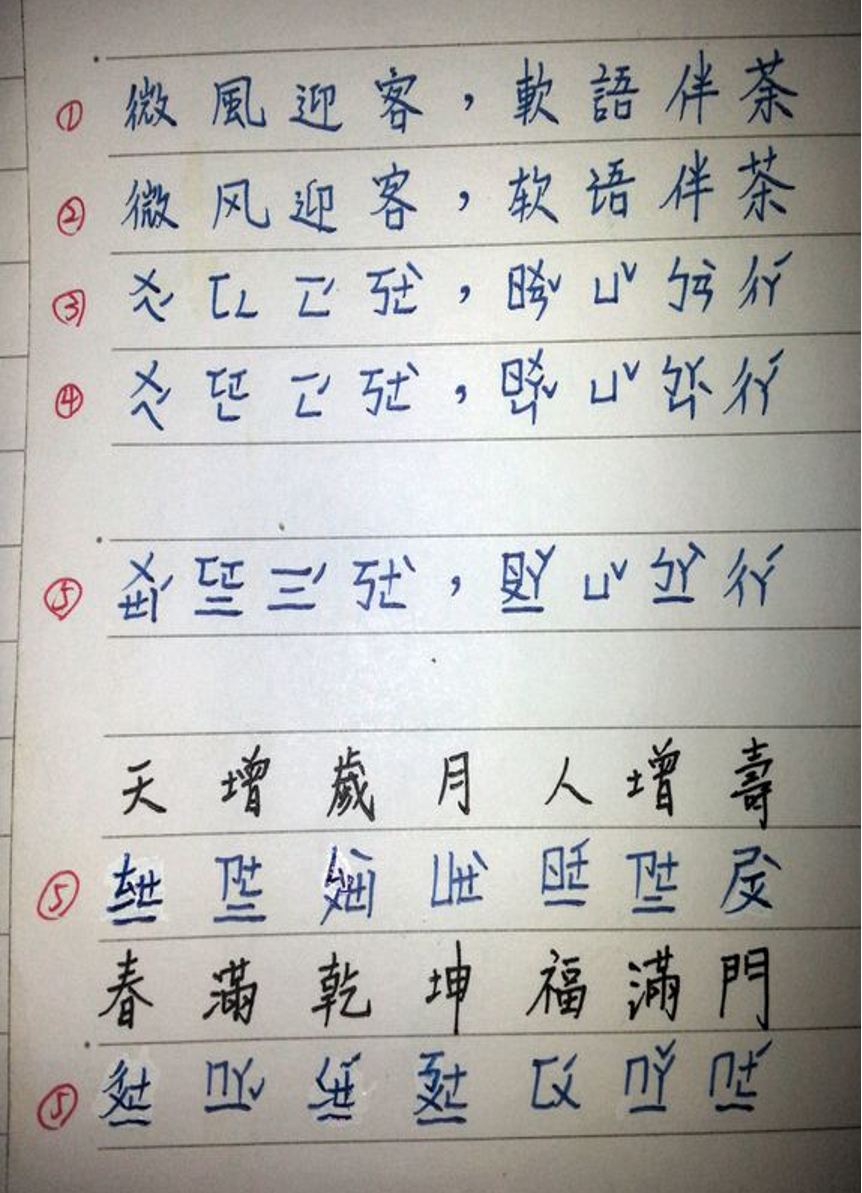
\includegraphics[width=0.8\textwidth]{./images/zhuyin_composed_4.png}
\caption{5yuidzeon的方案 注音方塊字設計圖 1繁體字 2簡體字 3直接寫成方塊字的方案 4將韻母拆分開來的方案(保留ㄞ 、 ㄟ 、 ㄠ 、 ㄡ四個韻母不拆) 5沿用表音方塊字韻尾的方案( ㄟ → ㄝ丨合字, ㄡ → ㄛ ㄨ合字, ㄣ →一, ㄥ →二)}
\end{figure}


\begin{figure}[h]
\centering
% 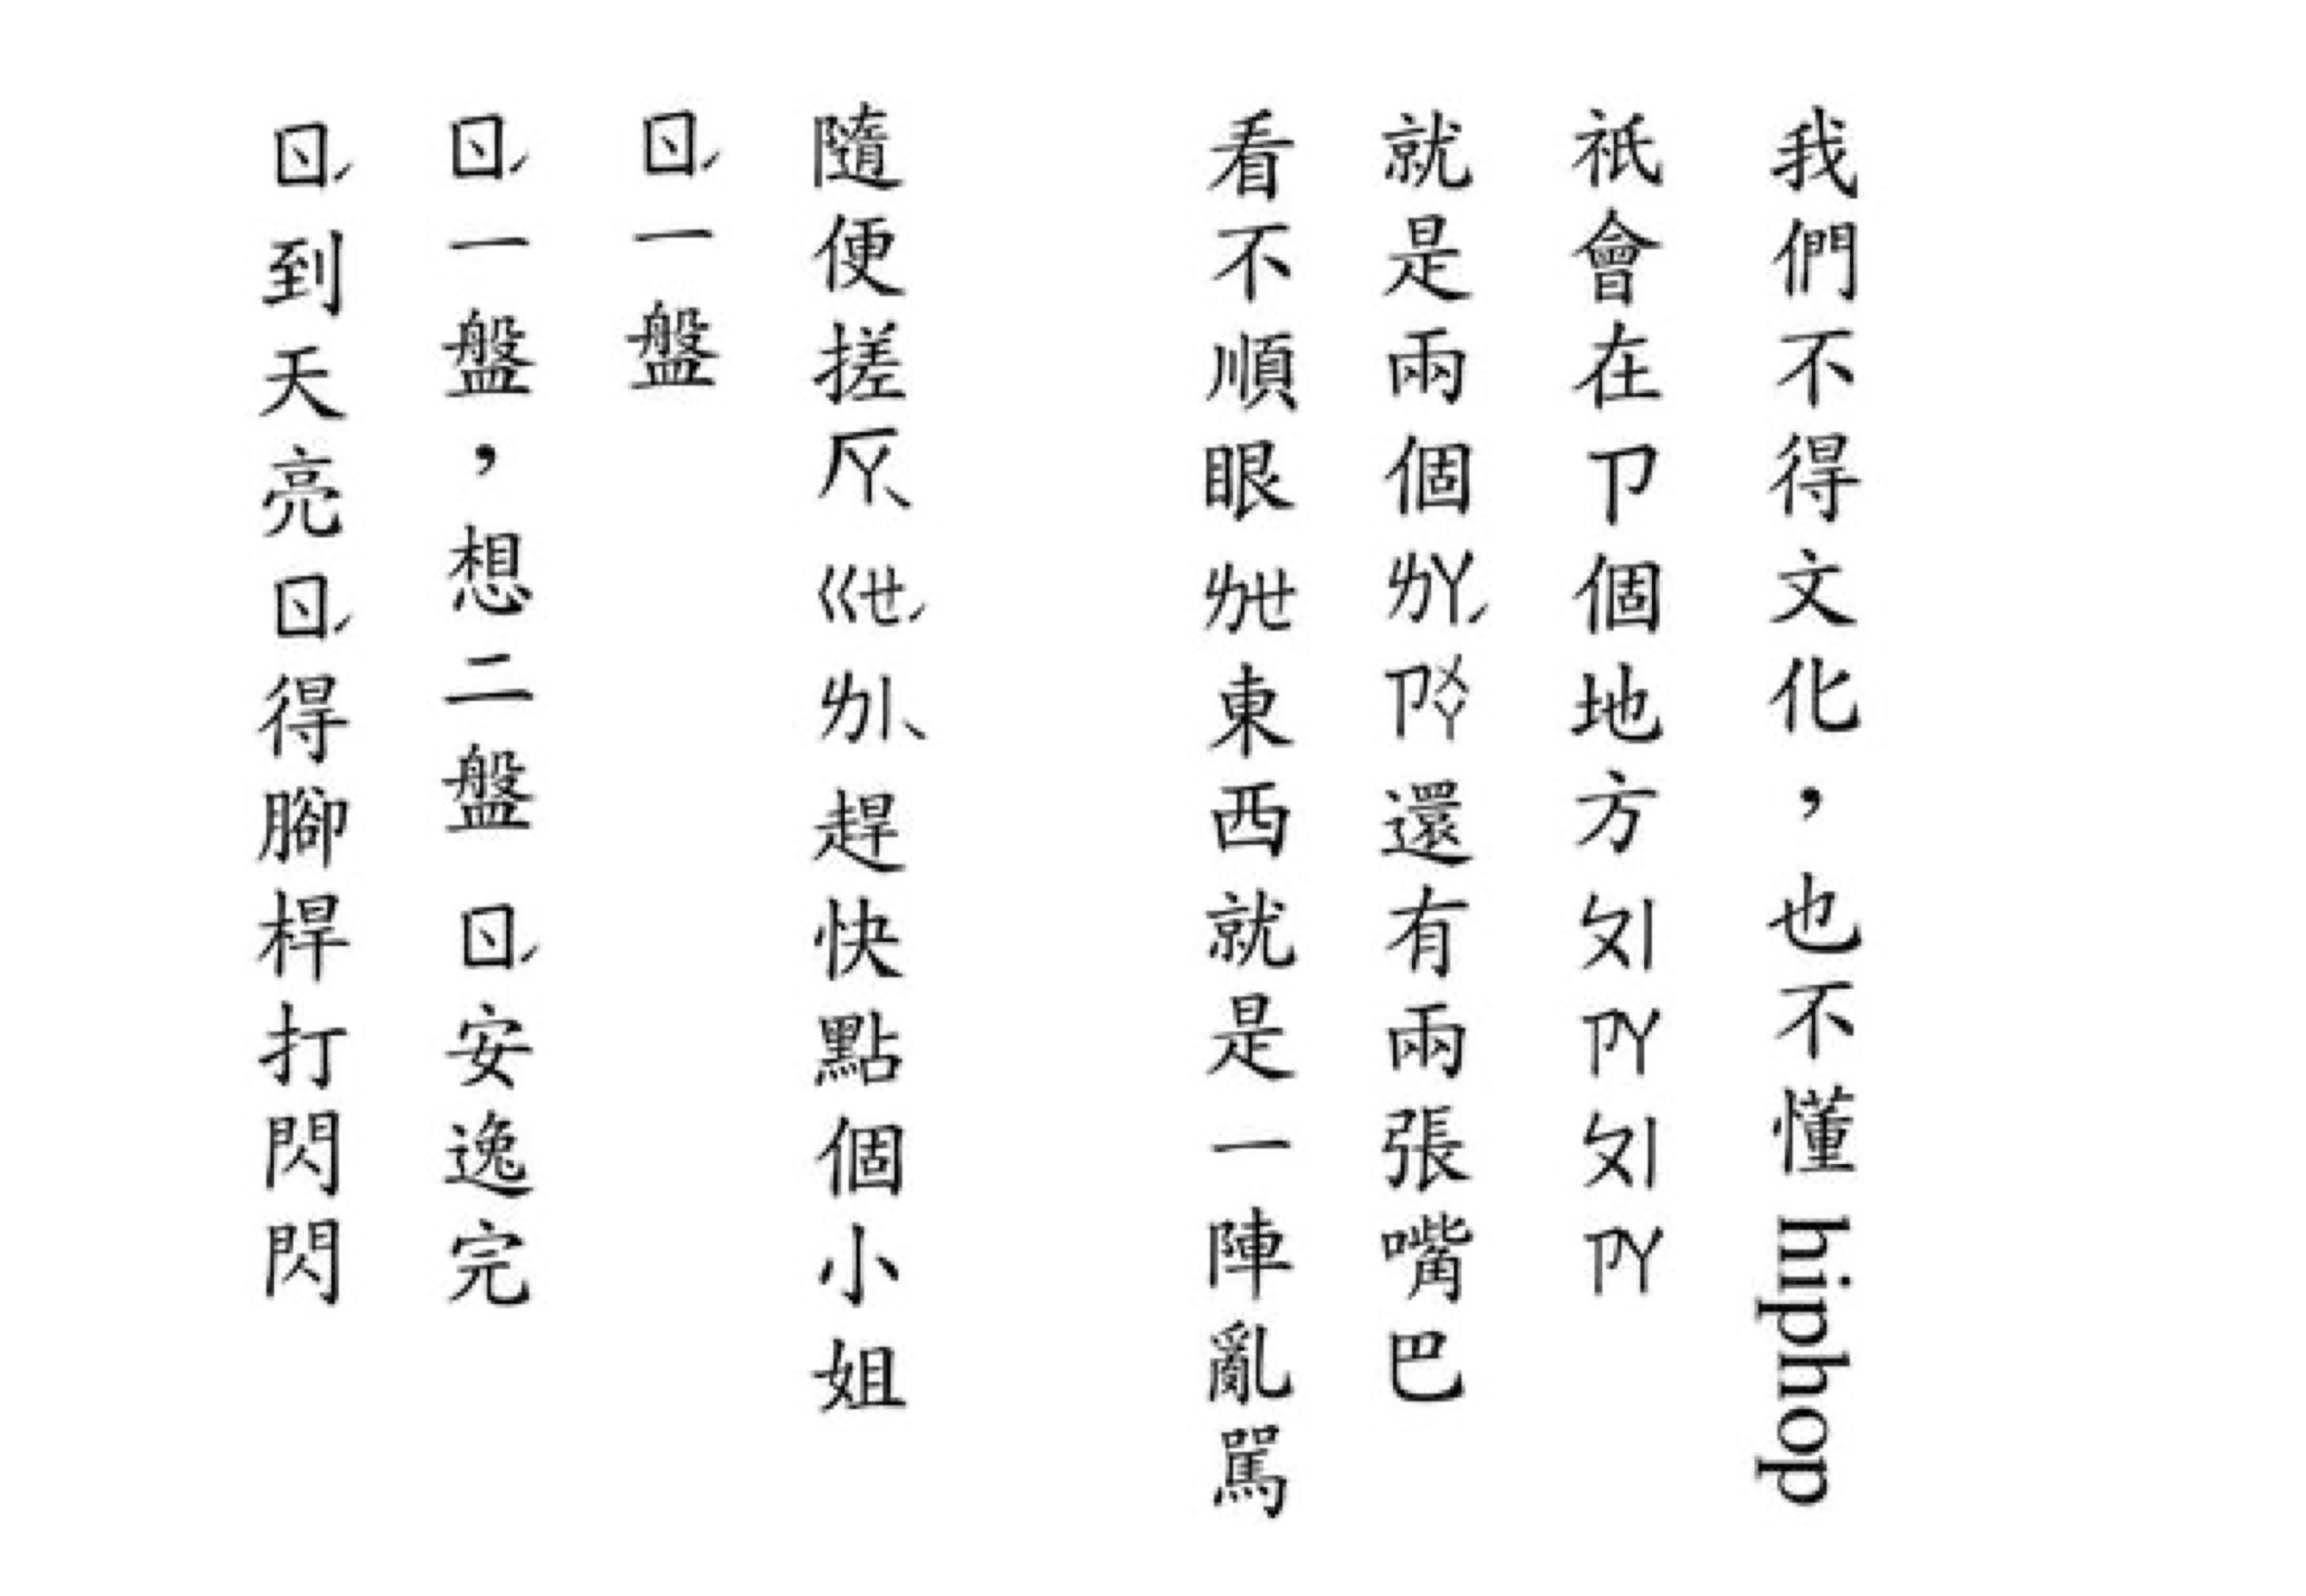
\includegraphics[width=0.8\textwidth]{./images/zhuyin_composed_5.png}
\caption{網友貼的一段注音方塊字例文:基本原則:左聲母右韻母 1.聲母在左,介音在右上,韻母在右下,聲調在右下,陰平不標調。 2. ㄧ單獨做韻母或單獨成音節時豎寫,其餘橫寫 3.半包圍結構聲母符號為了書寫比較方便,而產生了一些例外: a) ㄏ聲母字的介音韻母的部份寫到ㄏ右下 b) ㄇ聲母字的介音韻母部份寫到ㄇ下 c) ㄈ聲母字的韻母部份寫到ㄈ中 註:向左開口的半包圍符號如ㄅ ㄋ ,因為如果把韻母符號寫到包圍裏面去會違背最基本的左聲母右韻母原則,所以仍照規則1書寫。 4.介音+韻母類型的零聲母字(如ㄩ ㄢ )仍依規則1寫成上下結構,不將半元音視作聲母而寫在左邊。}
\end{figure}


把有注音功能的符號併合成為方塊字的方案,比較成功的有這個好像由一位叫 Aro 的人所發明的「布依族新方塊文」。可惜似乎完全沒有可以找到的出版說明書,只有網上圖片四幅,用例也只有一個,如下:

\begin{figure}[h]
\centering
% 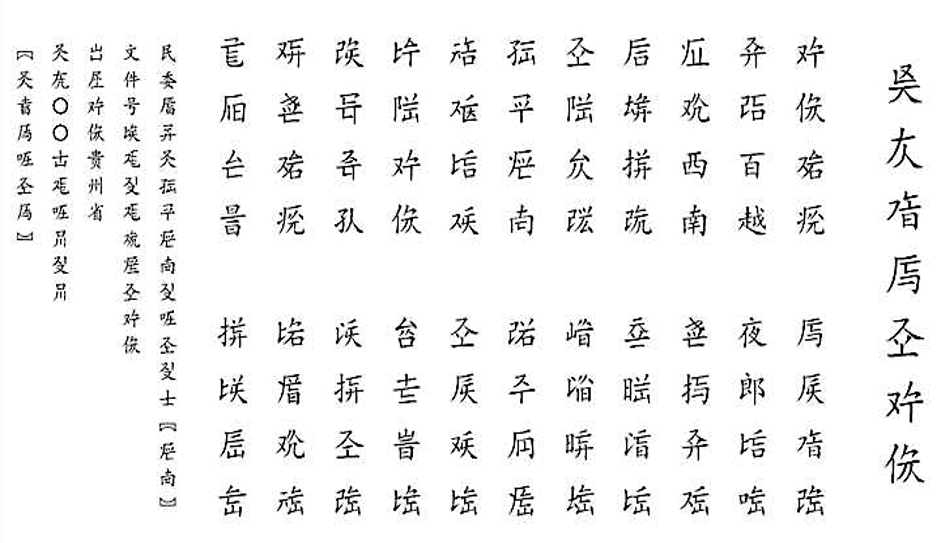
\includegraphics[width=0.8\textwidth]{./images/aros_buyizu_1.png}
\caption{布依族名溯源碑(布依族新方塊文):這個所謂「布依族新方塊文」的文字,網上的資料非常有限,不知道是什麼時候發明,也不知道有否某程度的通行。我首次發現其存在,是於https://www.zhihu.com/question/45320404/answer/166222552}
\end{figure}

\begin{figure}[h]
\centering
% 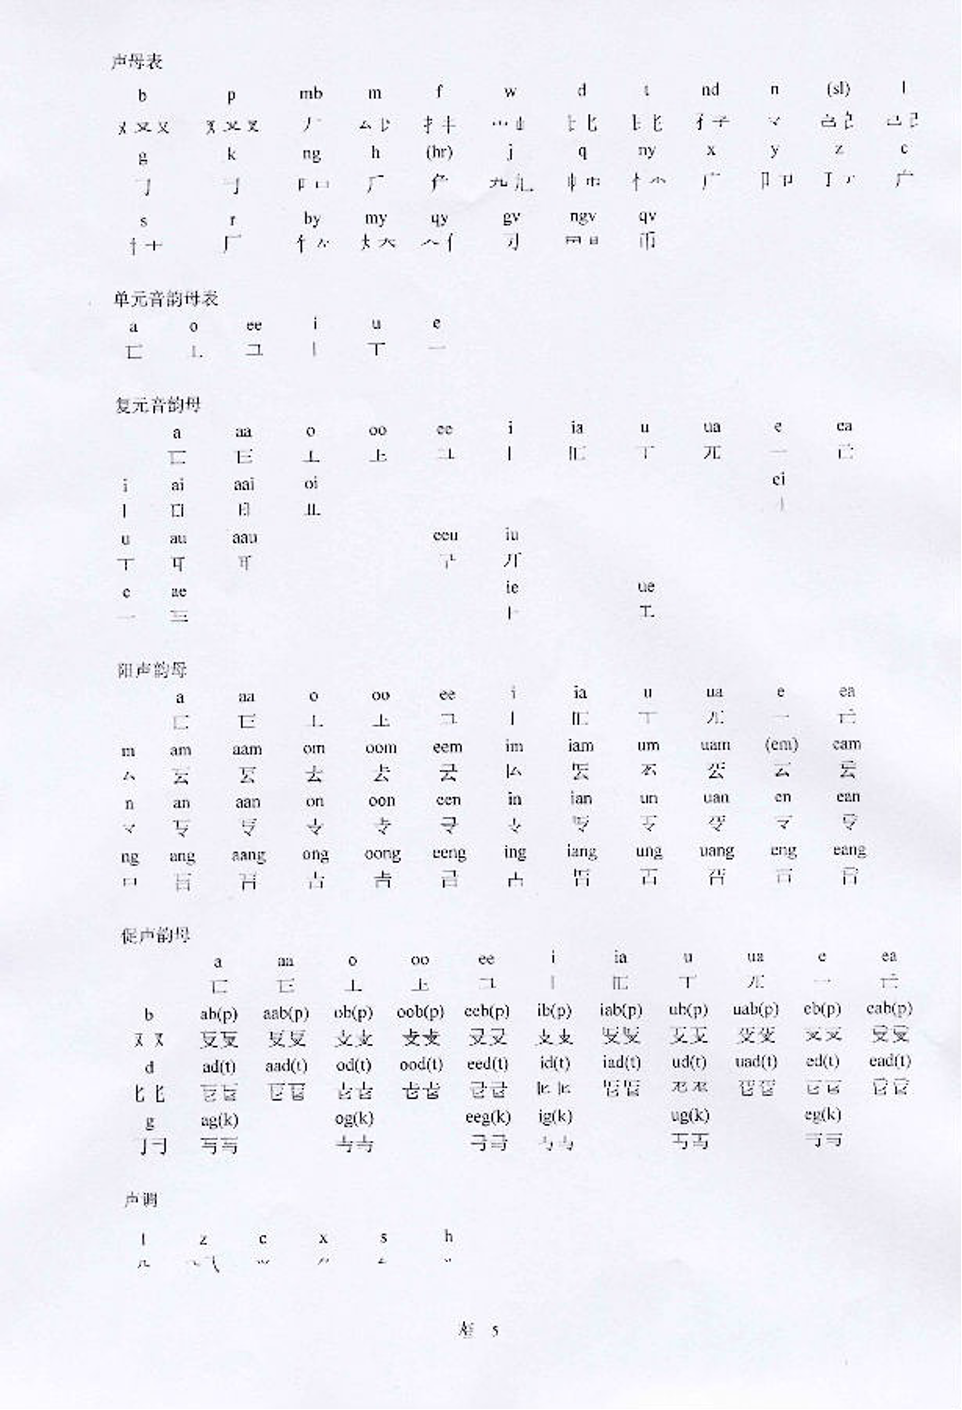
\includegraphics[width=0.8\textwidth]{./images/aros_buyizu_2.png}
\caption{布依族新方塊文併寫法(1)}
\end{figure}

\begin{figure}[h]
\centering
% 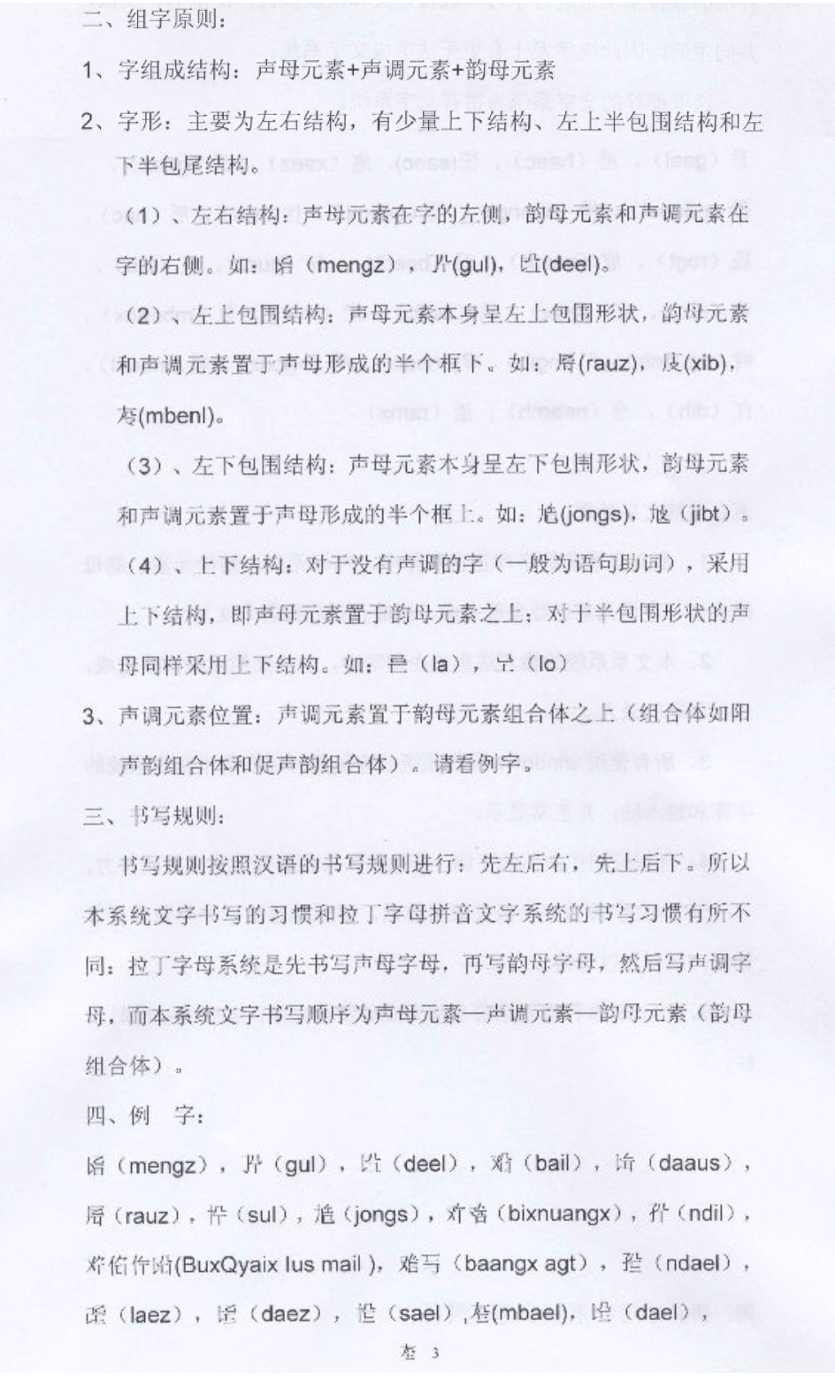
\includegraphics[width=0.8\textwidth]{./images/aros_buyizu_3.png}
\caption{布依族新方塊文併寫法(2)}
\end{figure}


\begin{figure}[h]
\centering
% 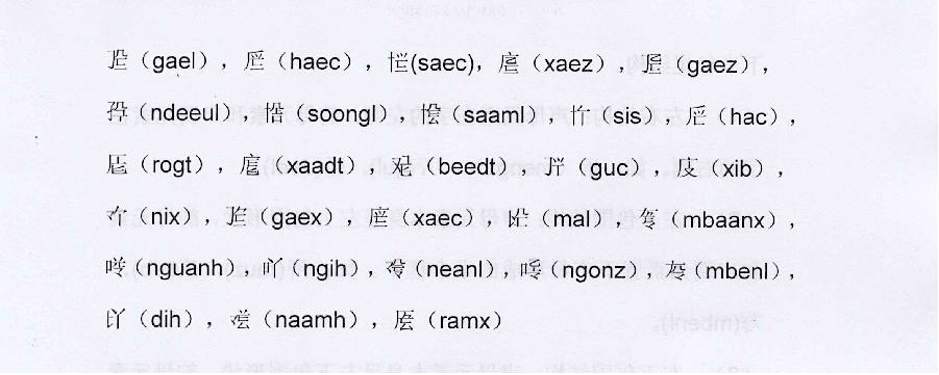
\includegraphics[width=0.8\textwidth]{./images/aros_buyizu_4.png}
\caption{布依族新方塊文併寫法(3)}
\end{figure}



布依族新方塊文的熵很高,因為他有四種併寫方法——聲母決定字型,然候韻母對號入座。我們還看到,韻母的符號不是完全沒有關聯的,而是相近的韻母,字符類似,方便記憶。而因為其發明家有考慮到整體併寫的規則與字符的相宜性,繼而修改符號的形狀,所以整體而言不會像注音合字那樣難堪不穩定,比較凝固。我們不難看到這些字都有「小字」的運作和設計影子。茲附上契丹小字以作參考。

\begin{figure}[h]
\centering
% 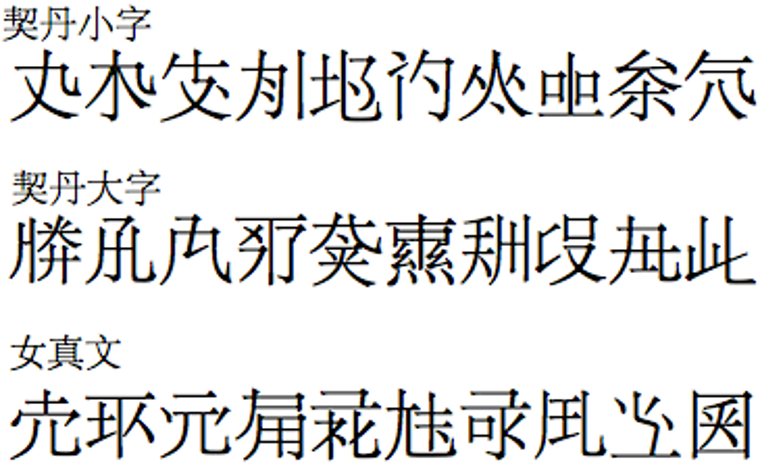
\includegraphics[width=0.8\textwidth]{./images/gujinwenzijicheng.png}
\caption{契丹大小字和女真文對比}
\end{figure}


\begin{figure}[h]
\centering
% \includegraphics[width=0.8\textwidth]{./images/khitan_1.png}
\caption{《大金皇弟都統經略郎君行記》,簡稱《郎君行記》,是金朝初年以契丹小字和漢字刻寫在無字碑上的碑文,記述金國皇帝弟弟尋獵於梁山的經過。題額用漢字小篆書寫。正文的契丹文部分有五行,97個字;漢文部分是契丹文部分的翻譯。這是目前發現的唯一契丹漢雙語文獻}
\end{figure}





要道出文為什麼這些「注音合字」方案通通都看起來醜得很,要在不浪費筆墨來闡釋一個關於文字美感的理論的前提下,不是一個容易的事。但這裡說幾點最明顯導致我們會方案的因素吧:一、部分的字符如「ㄚ、ㄛ、ㄨ」等非常難於方塊空間中遷就,導致不美。二、承一、這些的「注音合字」都看起來散修修,不能凝固自立,好像風吹一下就要散掉似的。之所以是這樣,因乎注音字母的形態不能互補陰陽,也就是說其設計沒有遵循漢字美感的一大理則。
圖 3的「道皃特點」就是注意到這一點,所「在註音符號的基礎上,對少數字母進行了修改。」三、表音的「ˉ ˇˋ˙」不夠崁入到注音合字的結構當中,有飛脫出來的感覺。四、部分的注音合字的熵不夠高,
圖 5、
圖 6都有這個問題。漢字的形態熵是非常高的,也是為什麼他美的一大原因。但
圖 5中的「天增歲月人增壽,春滿乾坤福滿門」的注音合字中的14個字中,有10 個都的底部都是以「一」字符為結構。熵可是一個非常重要的美感因素,而單純在這個範疇而言,注音合字連契丹文、和布依族新方塊字來的好。

% 如果把注音合字跟契丹文、和布依族新方塊字比較,注音合字跟契丹文最類似,但其實契丹文、和布依族新方塊字的熵都比注音合字高。注音合字跟契丹文都有嚴重的「散解性」,但也許契丹文比注音合字更嚴重——因為契丹文可以有超於三層的合併,合併之後字型拉長不再正方形而可以長方形。而契丹,和布依族新方塊字兩者比較,明顯布依族新方塊字最為成功,字型最穩,熵適當。注音合字如果真的要成功,就必須在字符的選擇上做到陰陽相合,但這個某程度上不推倒從來是沒有可能的。
% 表音方塊字
% 「表音方塊字網——中國表音文字研究交流平台」的最重要產品是「表音方塊字」。表音方塊字的基本運作就是直接把漢語拼音方案的拉丁字母的字符形狀漢化,用書寫漢字的筆畫來書寫拉丁字母,繼而併合。


% 圖 13表音方塊字系統說明。 
% 《世界人權宣言》第一條

% 人人生而自由,在尊严和权利上一律平等。他们赋有理性和良心,并应以兄弟关系的精神相对待。

% 《沁園春.雪》——毛澤東

% 北国风光,千里冰封,万里雪飘。望长城内外,唯余莽莽;大河上下,顿失滔滔。山舞银蛇,原驰蜡像,欲与天公试比高。须晴日,看红装素裹,分外妖扰。江山如此多娇,引无数英雄竞折腰。惜秦皇汉武,略输文采;唐宗宋祖,稍逊风骚。一代天骄,成吉思汗,只识弯弓射大雕。具往已,数风流人物,还看今朝。





% 《義勇軍進行曲》——田漢

% 橫寫		直寫
% 起来!
% 不愿做奴隶的人们!
% 把我们的血肉,筑成我们新的长城!
% 中华民族到了最危险的时候,
% 每个人被迫着发出最后的吼声。
% 起来!
% 起来!
% 起来!
% 我们万众一心,冒着敌人的炮火前进!
% 冒着敌人的炮火前进!
% 前进!
% 前进!进!		 

% 基本上表音方塊字不能成功的原因跟注音合字的原因一樣——太醜。設計上也有類似的缺憾。也許有點諷刺的是,表音方塊字是主要發明給普通話的,也就是今天的天朝雅言。但他使用的就只不過是漢化了的拉丁字母。沒有所謂的民族尊嚴之外,就是好像連自己的書寫習慣也沒有照顧。我們從上表把《義勇軍進行曲》以橫寫和直寫的兩個版本看到,這個表音方塊字其實用作來直寫是比橫寫好的——因為能夠避開那種數幾個字都底部有「一」字型的連貫效應。但這正正亦顯示了表音方塊字發明者的設計簡陋和不周——大陸是用橫書的。而任何一個粵拼字,必須橫寫直寫都得美感得宜。表音方塊字的設計,無能稱職。為什麼表音方塊字會出現這個「連一效應」?因為表音方塊字的前鼻韻母(an、en、in 、un)、後鼻韻母(ang、eng、ing、ong)的n 和 ng 在表音方塊字寫作為字符單位,分別為「一」和「二」,即如an安、en恩、yin音 、zun 尊、後鼻韻母ang昂、geng 更、ding 丁、yong 用。既然普通話中有這麼多的字都有前鼻和後鼻韻母,那就自然會做成這樣的「連一效應」。熵不夠高。

% 《學苑》中〈提升香港話地位——剝脫既定思想賦予口語詞彙書面寫法〉中亦建議不如使用粵拼為底層拼音系統,以拉丁字母為字符,以徐冰之書法和併合理則運作,製造「徐冰粵字」。以下為一些徐冰的「徐冰字」。


% 圖 14 用徐冰字體寫譯成為「文言式英文」王維的《鹿柴》:空山不見人,但聞人語響,返景入深林,復照青苔上。每一個字直譯為一個英文詞並繼而徐冰化。“Empty Mountain not see human; But hear human language echo; Returning light enter deep wood; Again shine green moss on.”

% 圖 15 徐冰新英文書法(毛澤東語錄)

% 圖 16 徐冰字母表
% 徐冰的嘗試完全是出於藝術考慮的,沒有任何實質語文政策的考慮。冒犯說句,儘管他的藝術品頗為好玩,作為文字是沒有民族尊嚴的。另外,徐冰的字貌似與漢字共和協調,但實質不然——他的美感太過西夏文的,而西夏文是宋朝金遼西夏三者唯一一個不是打字小字混用的國家,也是唯一一個是翻版漢字的文字系統。兩個美感如此「我都是漢字」的系統是不可以混用的。他們的美感相沖。一山不能藏二虎。
% 假名 

% 假名和諺文兩字系的最大問題就是他的美感具有非常強烈的文化個性,幾乎不容普世化和泛文化化。假名就是日本,諺文就是韓國——寫假名就是日文,寫諺文就是韓文。這個亦乃為何假名和諺文用作尾書寫粵語皆為不良的原因,假名或諺文來寫粵語都是不能為粵語提供一種獨立、具自尊、能命尊重、見而辨識的存在的。但當然,部分處理上海話字書化的人士認為吳語應用假名書寫。他們的理據很有趣,但其實是我給予的為何粵語不能使用假名和諺文的理由的另看。由於日語對漢字讀音體系有部分是源自大和時代從南朝建康周邊的吳語區借取,故此亦假名來書寫作為吳語代表的上海話,能拉近日語和上海話的關係。 

% 單純討論假名和諺文孰者較之適合粵語的話,肯定是諺文,因在入聲。假名用來讀寫入聲字有三種個方法:一、把入聲字的韻尾配上假名,然後照樣把入聲韻尾所配的假名的元音讀出來。這樣,如阿澤的例子,「虢礫緙嘞」就會變成「キックリックカックラック」,即「虢Kikku 礫rikku 緙kakku嘞rakku」。如此使用久而久之會潛移默化導致整個粵語的入聲體系壞掉,而且大量漢字要面對一個新發出來的雙音節化壓力。第二個的方法,也就是處理這個問題的方法,就是訓讀。但是訓讀是死記硬背,不能持久,雙音節化的壓力最終會勝出。第三個方法,就是把代表入聲韻尾的假名高寫以建立新的書寫原則,「虢礫緙嘞」作「キックリックカックラック」。

% 我個人認為這樣無論是哪一個方法,都太過複雜。其實日語假名是一個極度混亂的系統,工整性遠低於諺文。假名的混亂,是自然生成的,是天成的,是亂中有序的——可比英語的音系混亂和層層疊的例外的泛濫成災。日語假名之所以能夠於日本成功,是因為日本是一個島國,且有一億人,且有一千年的時間來發展和沈澱他們的語文約俗,發展出一種能夠駕馭此種複雜不堪(但又帶美感和邏輯)的三軌書寫體系,並生產大量的文學產品來奠基其語文質量和慣性。我們粵語沒有這些條件。
% 諺文

% 諺文,若非其「韓性」,其實頗為適合來書寫粵語的。而且已經早有人就諺文書寫粵語展開工作——香港城市大學的中文、翻譯及語言學系藺蓀先生之研究「訓民粵音」 ──以諺文書寫廣州話之嘗試》 為一大參考。也有用諺文來書寫閩南語,故此諺文寫粵語,並非首創。之後其設計理念又由黃得森在「訓民粵音」──以諺文書寫廣州話之嘗試》中闡發討論。 阿澤說他認為不用諺文的原因是現在粵語群的諺文拼寫能力為零,故此現實上走不了。但我考慮的不是源自政治現實的推行難度。我反對使用諺文的原因,不是諺文有什麼太大的缺憾。我反對使用諺文的原因,是諺文之所以偉大的原因。諺文之所以偉大,因為它是一個經過精密考慮,體大思精的造字工程。諺文不但崁入了大量的文化和哲學考慮到其文字設計當中,成宗在創造這個文字亦表現了亙古罕見的憂民愛民心態,甚至一種孟子民主主義的懷民情緒。在《世宗原詔》則可見成宗哀己民無字可陳書其意的情懷:

% 國之語音,異乎中國,與文字不相流通,故愚民,有所欲言,而終不得伸其情者多矣。 予爲此憫然,新制二十八字,欲使人人易習便於日用耳。

% 《訓民正音》序言亦曰:

% 有天地自然之聲,則必有天地自然之文。所以古人因聲制字,以通萬物之情,以載三才之道,而後世不能易也。然四方風土區別,聲氣亦隨而異焉。蓋外國之語,有其聲而無其字。假中國文字以通其用,是猶枘鑿之鉏鋙也,豈能達而無礙乎。要皆各隨所處而安,不可強之使同也。吾東方禮樂文章,侔擬華夏。但方言之語,不與之同。學書者患其旨趣之難曉,治獄者病其曲折之難通。昔新羅薛聰,始作吏讀,官府民間,至今行之。然皆假字而用,或澁或窒,非但鄙陋無稽而已,至於言語之間,則不能達其萬一焉。癸亥冬,我殿下創制正音二十八字,略揭例義以示之,名曰訓民正音。象形而字倣古篆,因聲而音葉七調,三極之義、二氣之妙,莫不該括以二十八字而轉換無窮。簡而要,精而通,故智者不終朝而會,愚者可浹旬而學。以是解書,可以知其義。以是聽訟,可以得其情。字韻則淸濁之能辨,樂歌則律呂之克諧。無所用而不備,無所往而不達。雖風聲鶴戾,鷄鳴狗吠,皆可得而書矣,遂命詳加解釋,以喩諸人。於是,臣與集賢殿應敎臣崔恆、副校理臣朴彭年、臣申叔舟、修撰臣成三問、敦寧府注簿臣姜希顔、行集賢殿副修撰臣李塏、臣李善老等,謹作諸解及例,以敍其梗槪。庶使觀者不師而自悟。若其淵源精義之妙,則非臣等之所能發揮也。恭惟我殿下,天縱之聖,制度施爲超越百王。正音之作,無所祖述,而成於自然。豈以其至理之無所不在,而非人爲之私也。夫東方有國,不爲不久,而開物成務之大智,蓋有待於今日也歟。正統十一年九月上澣,資憲大夫禮曹判書集賢殿大提學知春秋館事、世子右賓客臣鄭麟趾拜手稽首謹書。

% 諺文就是成宗的情緒的物體呈現,其發明成為了朝鮮文明的神話。但成宗的愛民的思想還不是它最偉大的原因,其之偉大在於它勇敢脫離了中國,成就了韓國。此非易事,畢竟你要脫離的是中國,一個極其宏偉霸氣的精神性秩序。故此,成宗發明推廣諺文,是一個更易文明,類似「脫亞入歐」的鴻舉,跟土耳其國父阿塔圖克(Atatürk)棄阿拉伯字母和越南的胡志明廢除漢字,意義一樣。但成宗是自創文字,猶如向宣告天下他自己存在,而不是「我搬家脫亞入歐了」。我們粵語如果要活下去,就必須仿效成宗這樣大膽的宏達志氣,否則我們不用打算在世界上有一席位,因為我們不配有一席位。故此,我們不能用諺文。我們要製造我們自己的諺文。


% 圖 17網上粵語發燒友發明的粵語諺文。 
% 清末民初表音方案

% 清末民初的切音字多如繁星。如上所道,基本上倖存真的被採用為官方文字、有社群使用的文字,只有注音符號。但這並不意味他們沒有參考的價值。參考的價值非常豐富,除了老生常談的「失敗乃成功之母」之外,原因有以下:一、他們失敗的因素——政治、文化、運作、美感上,都是珍貴的材料;二、他們推廣自己的方法仍然值得參考——而當中一點非常重要的就是閱讀材料,尤其是範文、教科書、閱讀文章的出版。這個推廣方式非常重要,但在我們的世代可能已經習以為常,覺得理所當然,沒什麼大不了。可知道——白話文最初的推廣,其中最為重要且好大的工程,就是白話文文章的出版。這一個值得參考。三、就算完全沒有參考價值,知道他們的存在以及其存在的多樣和規模,證明著這個曾經是一個浩浩蕩蕩,幾乎所謂大勢所趨的勢力。他們的失敗,不是必然的。如若此,則意味我們是有機會成功的。以下是剽竊自王東杰著的《聲入心通——國語運動與現代中國》的「清季切音字方案一覽表」:

% 作者	年份	著作或方案	字母形體	拼音標準
% 盧翰章	1892	《一目瞭然初階》 
% 《新字初階》 	拉丁字母及其變体	廈門音、漳州音、 泉州音
% 吳稚暉	1895	「豆芽字母」 	漢字筆畫
% (獨體篆隸及變體)	無錫音
% 蔡錫勇	1896	《傳音快字》 	速記符號	官話音
% 沈學	1896	《盛世元音》 	速記符號	吳音
% 力捷三	1896	《閩腔快字》 	速記符號	福州音
% 王炳耀	1897	《拼音字譜》 	速記符號
% (有大拉丁字母對音方案)	粵音
% 蔡元培	1898	《切音課本》	漢字(韻書)	浙(紹興)音
% 王照	1900	 《官話合聲字母》 	漢字筆畫	官話音
% 田廷俊	1901	《數目代字訣》	數碼	湖北音
% 力捷三	1902	 《無師自通切音官話字書》	速記符號	官話音
% 陳虯	1903	 《新字歐文七音鐸》 《歐文音匯》 	漢字筆畫	浙(溫州)音
% 劉孟揚	1904	《天籟痕》	漢字筆畫	官話音
% 李元勳	1904	 《代聲術》 	不詳	不詳
% 楊瓊、 李文治	1905	《形聲通》	漢字筆畫	韻書(?)
% 曾杏村 	1905	《嶺東新字母》	不詳	不詳
% 勞乃宣	1905 1906	《增訂合聲簡字譜》《聲簡字譜》《簡字全譜》 《簡字譜錄》	漢字筆畫	寧音、吳音、閩廣音
% 盧翰章	1906	《中國切音字母北京切音教科書》
% 《中國字母北京切音合訂》	漢字筆畫(有拉丁字母對音方案)	官話音、泉州音、漳州音、福州音、廣州音
% 朱文熊	1906	《江蘇新字母》	拉丁字母	吳音(後另訂官話音方案)
% 田廷俊	1906	《拼音代字訣》、《正音新法》	漢字筆畫(有拉丁字母對音方案)	湖北音
% 沈韶和	1906	《新編簡字特別課本》	數碼	韻書(?)
% 邢島	1906	《新漢字》	不詳	不詳
% 貴翰香	1907	不詳	漢字筆畫(?)	浙音(?)
% 江亢虎	1908	《通字》	拉丁字母	官話音
% 劉孟揚	1908	《中國音標字書》	拉丁字母	官話音
% 馬體乾	1908	《串音字標》	漢字筆畫	官話音
% 章太炎	1908	《駁中國改用萬國新語說》	漢字筆畫	韻書(?)
% 宋恕	1909	《宋平子新字》	漢字筆畫
% (模仿日本假名)	浙(溫州)音
% 劉世恩	1909	《音韻記號》	自造符號	官話音
% 黃虛白	1909	《漢文音和簡易識字法》	漢字筆畫	官話音
% 黃虛白	1909	《拉丁文臆解》	拉丁字母	官話音
% 萬雨生	1909	「中國音字」	不詳	不詳
% 鄭東湖	1910	《切音字說明書》	漢字筆畫	韻書(?)
% 吳稚暉	不詳	「省便反切字母」	漢文	不詳
% 陳貽範	不詳	《號碼代字捷訣》	數碼(?)	不詳
% 趙嗣璹	不詳	「拼音新字」	雜取各國(拉丁字母)	官話
% 表 1《聲如心同》——清季切音字方案一覽表。 
% 這個表並未包含所有寒夏民國的拼音化方案——清朝內的還沒全部包括,譬如Tarleton P. Crawford 為上海話發明的文字系統,焉其者的著作有《上海土音字寫法》、《A system of phonetic symbols for writing the dialects of China》、《善惡經》等。中共蘇維埃於1928開始研究發明推廣的「拉丁化新文字」(Latinxua Sin Wenz)也不包含在內。還有西方傳教士為南方諸語發明的拼音方案。有些非切音但其實或有參考價值的方案,如趙元任發明的通字方案(General Chinese)也沒有被錄於表上。

% 這些方案大部分的問題都跟注音符號的大同小異,其弊不重複。

% 清末民初坊間出現大量方案,現時仍然偶爾有方案鋪頭。如上文已經提到的「表音方塊字」和種種的「注音合字」。這裡,我再討論幾個值得參考的系統。這些系統之所以值得一提,大多是因為他們的都不至是某種把拼音系統字符更換掉就完成的系統——他們的設計都彰顯了其發明家不同的考慮。更重要的是,以下的三個方案,讓墨文、吳語小字,嗒字,都有超於字符,有文字系統層面的的設計考慮。
% 讓墨文

% 讓墨文是一個由夏修文發明的拼音文字系統,基本是小字方案。 

% 普通話的讓墨文方案基本上是把漢語拼音方案的拉丁字母重新配上字符,而這些字符則按照讓墨文的併合規則,組寫成為一個一個的讓墨字。我們在此貼上讓墨文的普通話拼寫法,附錄中會包括其其他漢系語言的拼寫方案。

% 圖 18讓墨文拼寫例子。
	
	

% 圖 19讓墨文併合規矩。





% 圖 20 kuang 與chuai 的讓墨文



% 圖 21 讓墨文

% 圖 22 讓墨文官話拼寫方案。

% 圖 23 讓墨文粵語併寫系統
% 讓墨文有幾點的特點:一、他標調,而表調的符號是一個跟元音輔音等體、地位相等的。它不像注音符號,音調以某種的附加符號(diacritics)來表示,而是一個自有地位的字符來表示。二、承一,讓墨文的標調是強制性的。這個有別於注音符號。注音符號是可以不表調,但字的書寫拼合仍為完整。但讓墨文不可以不標調——不標調讓墨文的字不能完整寫成。三、夏修文把讓墨文的符號系統經更改微調後,用其字符為其他的語言,如粵語、贛語、日語、韓語等建立了相應的讓墨文系統。四、讓墨文的主要書寫模式是方塊合併寫,但亦能線性寫。五、如夏先生自己所述,他考慮到美感的問題,字符是特別按照漢字美感理則而選的——已經顧慮到併合之後的型態。故此,讓墨文完全沒有注音合字的那種不穩鬆散的感覺。

% 但讓墨文有幾個問題,且頗為嚴重。

% 一、讓墨文的學習成本非常高——因為所有的字符都是自創的,沒有歷史根基——這一點比清末民初的許多切音字還要差。清末民初很多的切音方案,比如注音符號、王照的官話合聲字母等中的字母,是取自漢字篆體或異體,經修改而成的——故此不但有(一定的)文化上的連貫性,用家能夠透過把新字符的讀音跟其修改自的漢字建立邏輯上的關係而漸漸學會使用。但讓墨文完全沒有這一個操作,只能死記硬背。在這一點,它遜於諺文、假名、注音。

% 二、部分的字母跟漢字部首重疊。

% 三、標調:使用漢字的人多數都講某種的漢系語,而漢系語言大多都有音調系統——但這不代表我們時時刻刻都的語文習慣都離不開音調。當我們看看我們的語言直覺是,就會發現其實我們對漢字語素的元音輔音的自然把握是頗為敏感的,但是音調卻不嚴謹。音調的確有辨義作用,但我們要辨別一個音調是什麼,卻比我們要把那個音調所依附的音素合併是對應著哪一個語素來得困難。要說明兩個調是不是有分別很容易,但是要辨別一個調的身分是什麼卻很難。

% 當然,這個現象是取決於我們的語文習慣的,也就是說是可以更改的,也可以習慣的。普通話為母語的人,從小到大就學習漢語拼音,故此要拿捏聲調可能比比較容易。泰文,也會強制標調。但粵語從來都沒有這樣的習慣,故此如果要引入此習慣,就得對抗我們的現有語言習慣。這樣對短期上的推廣是不利的。而觀乎墨文,由於漢語拼音歸根究底不是正式的文字系統,而只不過是一個輔佐的表音系統,故此也未真正成功把辨調的習慣注入到使用家當中,故此強制標調以及調符和表音符地位等同的設計,就導致讓墨文的書寫變得非常不直覺,要透過訓練才能成事。這一點也暗示著,一個應當成功的粵拼字系統,是不必硬性標調的。讓墨文的音調和元音輔音的符號是同階級的,茲乃其敗筆,亦乃其必敗的原因——因為這個太過違反了我們習慣了的文字習慣。可知道——漢字不表調,用讓墨文不但要學習如何表調,還要發展出一個完整自如的辨調觸覺。不是不可能,而是成本高,麻煩,故此容易失敗。茲給我們的教訓,如果我們的粵拼字要跟漢字混用的話,要減低推行成本的話,就必須儘量使用漢字的操作機理,扭曲時不能過分,否則過曲則折——那完全廢除漢字反而可能變相成功機率更高。
% 吳語小字

% 吳語小字(又稱「吳越小字」)是一個由一位網名為Narihato Ohfu成鳩王鈇 所創造的文字系統,用於來書寫吳系諸語。其輸入法也業已公開。 其介紹為:

% 小字是受到梵文天城體、韓語諺文的啟發,參考中文注音符號和日文片假名,運用漢字部件的組合來表音的音素文字。它區別於一般表意正字,既適合像普通話的注音符號那樣給漢字進行注音,也能夠像日文的假名那樣入文混寫。引入小字,可用於無字詞彙、虛詞的記音和外來詞彙的音譯,同時可避免漢羅台文那樣由羅馬字母與漢字混寫所帶來的弊端,尤其適合豎排文字的排版。

% 小字音素表的羅馬字母方案參照的是通用吳語拼音,適用於北部吳語區的大多數地區,運用韻尾標記也能適用於大多數南部吳語區。 

% 成鳩王鈇亦提道:「在漢字小字混用的時候,有點像朝鮮的諺文—漢字並用和日本的假名—漢字體系。吳語小字方案,是一種注音、輔助工具,用來標記虛詞和語法標識,讓吳語書面文本中的句子結構成份更加的清晰明瞭,避免了漢字實詞、虛詞不分對句子成份分析所帶來的干擾,為吳語的高階化打下了工具基礎。」吳語小字,其名為「小字」,是繼承倣傚契丹小字、女真小字字等「均是以類似漢字偏旁部首的表音符號來拼寫發音」的文字系統而設計的。理論上,目前版本的吳語小字之中,可以組合出 上字(38+1)x下字(26+1)-1 = 1052個字元。  



% 圖 24 「歡迎學習吳語小字」吳語小字標音。

% 圖 25 反送中吳語小字文宣



% 圖 26用吳語小字跟漢字混用書寫的芥川龍之介《蜘蛛絲》,直排本。


% 圖 27 用吳語小字書寫的吳語版芥川龍之介的《蜘蛛絲》(橫排版)。

% 圖 28 《願榮光歸香港》吳語小字版

% 圖 29吳語小字拼寫規則暨使用規則撮要,取自https://www.zhihu.com/question/276483154。或非最新版本。

% 吳語小字設計的特點非常多,其設計選擇非常強烈地彰顯著其他朝成為正式官方文字的意志,亦彰顯了成鳩王鈇對吳系諸語的語言及文字的理解、發展願景藍圖,甚至漢字語文的運作理則。吳語小字,是一個極度了不起犀利結棍的偉大發明。

% 一、設計美觀,比契丹、女真、和注音都要成熟,也充分保留了天城文的運作理則和美感,但又漢化得宜。美感有過假名、諺文而無不及。

% 二、用以跟吳語小字混用的漢字是繁體字,而非簡體。成鳩王鈇之所以這樣選擇,毫無疑問是為了將漢吳混寫的語文美感最大化——茲亦印證了漢字使用家一致認為繁體字美感勝於簡體的共識。

% 三、吳語小字,顧名思義,是(幾乎)通用乎於諸吳方言的,這個文字系統完全沒有預先設定了一個吳語的威望方言(prestige dialect)。這個設計應該是故意的,背後原因非常深思熟慮,考慮周到。

% 成鳩王鈇在設計吳語小字時,方法是先選定一個吳語的拉丁化方案,再繼而更改字符——更改字符的模式不是把拉丁字母一對一投射至新的字符,而是把音素作為底層單位字符化。而他選用的吳語拉丁化方案乃吳語協會的「通用吳語拼音」。通用吳語拼音,顧名思義,是吳語的通用拼音,特長在於可以貫穿大量吳語方言的拼音系統——通用吳語拼音,適用於北部吳語區的大多數地區,運用韻尾標記也能適用於大多數南部吳語區。這一點很重要,通用吳語拼音真的包涵是整個「吳語區」的拼音方案,而不是如「法吳」以上海話作為吳語的代表,為上海話發明了拼音之後就篡位,身分為上海話卻自稱吳語拼音。通用吳語拼音之所以真正能夠通用於整個吳語區,是因為他的設計方法,是先把不同的吳語方言的音系考察出來。不同的吳語方言會有不同的音系,亦即有些吳語方言會共有某些的語素,跟其她則不必然。把所有的音素整合之後,就在一串拉丁字母配一個音素。這樣,通用吳語拼音就真的能一擊即破大量吳語方言——而不是只為吳語中最為強勢的上海話服務,並以上海話為吳語以壓迫其他吳語方言。由於吳語小字是建基於通用吳語拼音,故此,吳語小字也是能用來書寫所有吳語方言。而正正因為要以一個自我整全的文字系統來書寫大量吳語方言,吳語小字的系統是元音附標文字 (abugida),類似天城文。因為這樣,類似的元音-輔音對子,只要把元音符稍微更改,就可以得出新的元音-輔音對子字符,學懂了一個吳語方言的書寫,要轉移到另外一個吳語方言,學習成本也不至於壓人於不可發。使用時吳語小字,用家不用也用不著所有的字符,只需把自己的吳語方言中有用的音素的吳語小字部件抽出來,其他置諸不理。亦即,每個吳語方言,從吳語小字中抽出符合自己的子系統,即可。

% 成鳩王鈇以通用吳語拼音,而不以吳語最強勢的上海話為主體作為設計的本參語言,是明顯出於對整個吳系語言的發展考慮的。其思路也許有點與大眾直覺逆向,但對我們粵語的發展仍有非常巨大的參考價值——儘管也許我們最終不會跟隨他的選擇。首先,成鳩王鈇認為上海話已經嚴重的潰敗,幾乎不能擔任承載吳語文明的能力。這不是因為上海話是一個非常年輕的吳語,不是因為上海話本身是一個集蘇州、寧波的柯因內語(天成折中共同語)使其之喪失了吳語本有的特質(雖然斯語確然,而他亦相信不會完全否認),而是因為自改革開放以來,甚至自民國時代,上海話受到官話,尤其是普通話的影響,使他的內部語言特徵全部向普通話靠攏——亦即趨同。而這個趨同,是惡性的,因為他認為普通話是一個不精密且結構簡單,繼而不利思辨,甚至乃一礙於敵於理性的語言。這種向官話靠攏的現象,他稱之為「藍青化」。

% 「藍青化」發生於上海話的音系上,故此出現中派和新派上海話。詞彙也出現棄滬取普的現象。文字出現「普字滬語」的現象,民眾喪失使用漢字書寫上海話,或失去用上海話閱讀漢字的能力,均乃藍青化。而最重要的是,藍青話導致滬語的整個語法系統急速簡化,拋棄了原生上海話和吳系諸語的原生語法——如格、時態、事態、形容詞分級等等。而這些語法上的複雜性和多樣性,是理性思考和邏輯思辨的重要工具,甚至發生原地。故此,如果以上海話為軸心來處理整個吳系語言的字書化,會最終因吳語的上海話化而導致整個吳語文明思哲的潰敗。相反,以通用吳語拼音,則可以為滬語之外的吳語提供自身安全的空間,發展和探討自己語文的發展,並好好利用自己原生語法,在思哲上推進。在這個情況下會不會出現柯因內化則比較難說,成鳩王鈇認不認可在這個前提下產生不是源自已經藍青化的滬語的柯因內語,亦是一個難答的問題。但無論如何,就算是要出現吳語柯因內語,這個原生沒藍青化的吳語柯因內語,也必一個已經藍青化的柯因內吳語好。

% 四、成鳩王鈇以吳語小字為骨幹的復興吳語工程,發明吳語小字只是一部分,而在他觀點,更重要的是語法的梳理。發明了吳語小字,吳語就可以寫了——但如何寫,成鳩王鈇認為需嚴格調控,透過專制的語法梳理工程來奠基,成功之後才能開放使用權。也就是說,成鳩王鈇把構建書面語和創造文字系統的工程集合為一了。為什麼要進行語法工程?原因大概有三。一、一些很可理的建議書寫規矩,無可避免產生了此需要——譬如;吳漢混文,實詞寫漢字,虛詞寫小字,非常自然可理,但這樣就需要處理什麼是實詞,什麼是虛詞,而這一個又在牽涉到什麼是「詞」的問題。而這一個問題,看似簡單,但其實內裡藏凶,是一個非常麻煩的漢系語言語文學的難題。二、不作語法梳理工程就開放使用,會導致沒有導向盲頭烏蠅的過早約定俗成發展,會讓吳語的書面語構建工程走很多冤枉路,浪費大量文學精力。三,承二,如果貿貿然開放使用,並沒有統一經過思考和分析而定的規矩,吳語語感已經大為衰退的吳語人就會以吳語小字寫普通話化了的吳語。這樣吳語小字反而未必會防止進一步藍青化,反而會使藍青化變得無可挽回,原生吳語無力回天。所以,要重塑吳語語法,讓使用時吳語能真正綺麗自立。茲茲考慮,就是要確保吳語白話文會是真正是「吳語」是「白話」的「吳語白話文」。而如在上文的語法整理工程討論中所道,語法整理是釐清思路的重要一步,吳語小字的發明就正正納入了此工程了。整理了語法體系之後,漢字和小字的書寫職責就變得明顯、自然、理則所逼而無可爭詏。


% 圖 30 吳語小字作為釐清吳語語法的示範 

% 成鳩王鈇為什麼選擇漢吳混用而不純用吳語小字(而廢漢字)的理由也非常有趣:

% 問:像越南或韓國那樣採用全拼音文字,有哪些缺點?為什麼其他語言完全採用拼音沒有問題,(前)漢字圈諸語言卻不行?

% 答:漢字圈文化的語言都受到中古漢語、近古漢語強烈的影響與滲透。漢字詞彙大量地置換了這些地區的原生詞彙,漢字已經作為詞根的形式深度紮根與這些語言的詞彙中。而漢字詞根比較的簡練,導致重音律高,全拼音化的結果會造成同音異議詞變多,尤其是朝鮮語,拋開漢字後閱讀都會造成一定的障礙。再加上東亞語言詞彙的虛詞詞根部分特徵不明顯,全漢字導致虛實詞難以區分,全拼同樣會造成虛實詞難以區分。這一點採取實詞用漢字,虛詞用假名的日語構建是最好的。
% 除此之外,漢字圈文化中詞性標記整理的相對好的是日語和朝鮮語,前者雖然有大量的訓讀但問題是音素太少,後者則是全文讀系統,這都導致全拼情況下記憶詞彙會變的困難。但這些其實都不是最嚴重的問題,真正的問題在於全拼後導致文化的割裂,今人無法很好的繼承祖先的文明傳承。大量文明信息因不懂漢字而造成根源上的丟失。這一點朝鮮半島人和越南人深有體會,這兩地文字改革後一直沒有出現著名的文學作品也從側面反映了這一點。 

% 此外,他亦解釋了為什麼他認為普通話的滲入,是會導致思想堵塞。

% 問:先不論吳語未來如何,請問你怎麼看受到官話思維影響的諸語言,未來會如何發展?官話本身未來如何?使用這些語言的人,在可預期的未來,將因官話思維深受其害,而不自知?

% 答:首先官話和普通話不是同一個概念,儘管英語對於兩者的解釋都是Mandarin,它包含了官話與普通話。
% 普通話是官話的2.0版,融入了更多英語語法的建構成分(儘管這種吸收和建構非常失敗)。Mandarin未來能發展到如何我無法預言,但我相信以這種語言為母語的人群在思維邏輯上以及思辨能力肯定是不如屈折語和黏著語母語的人群的。妳不可能讓一個對時態、語態、事態、格、屬、性毫無概念的人能在根本的思維層面上明白和運用這些,而這些又和邏輯思維、思辨力息息相關。
% 簡單來說Mandarin到目前為止都沒有很好的整理出一套可以自圓其說的語法。所以以Mandarin為母語的文明中出現思維精神分裂的縫合怪非常的司空見慣。不借助其他邏輯思辨更強的語言作為思維工具,單憑Mandarin甚至連學習高等數學都會十分喫力,成才率也更低。
% 從這個方面來說,大眾爭論不休的是否廢除漢字的討論其實倒是很次要的問題。東亞諸國書面語離開漢字是非常不現實的,但用全漢字作為書面語表述工具是會阻礙語法建構和思維發展的。 

% 我不太認同他對普通話的評價。成鳩王鈇認為普通話是一個會導致思哲混亂,或本身不能承載高質思哲活動的語文。我不認同。我認為普通話在清末民初以來一直快馬加鞭搶借西方語文的結構和詞彙來提升自己(所以才說「到目前為止都沒有很好的整理出一套可以自圓其說的語法」),是的確有成果的,而那些成果是真的。我們不能肯定或說清成鳩王鈇會否認同此見。他說普通話作為一個「這種吸收和建構非常失敗」,我能明白相對而言,和觀乎泰西語文本有的理性和語法而言,普通話的吸收和建構的確未能複製到泰西的理性和語法精密,但成果是有的。有成果,跟成果在絕對尺度上是否夠大,乃相關但分離的問題。此外,他不能否認,普通話這樣的構建,是諸漢系語中最為成功的,遠超粵語——因為粵語有那些否定「西化中文」的文人遺老。我認為,普通話的構建整體上,效果是有且巨大的。

% 為什麼不能完全脫離漢字?出於不現實。但這個其實不是回答的重點。重點在於為何成鳩王鈇不能仍欲廢除漢字的原因——因為漢字導致其語言用家的語文出現惡變,導致思辨的潰敗。

% 問:漢字為什麼會導致理性思辨崩毀呢?當中的運作機理和前因後果是什麼?

% 答:漢字不會導致邏輯思辨出現障礙,但文本用純漢字表述會導致邏輯思辨的混亂。理由如下:
% (1)漢字基本都有實意,當漢字作為虛詞成分出現時,它的基本實意會干擾解讀者理解它作為語法標記時的作用和意思。全漢字文本讓虛詞、實詞的區分和識別變得困難;
% (2)虛詞、實詞難以區別和辨識就會導致語法建構出現問題,難以形成自洽的語法體系,甚至讓很多漢語母語者以為漢語沒有語法;
% (3)漢字的延展性導致了大量的望文生義,特別是成語、習慣語的字面意思模糊,非常容易導致不同時代背景的解讀者朝著相反的方向理解,著名的例子有「七月流火」、「空穴來風」、「不孝有三、無後為大」。以上這幾個問題相互交織疊加讓漢語的語言思維更是變得混亂不堪,直接導致漢語母語者多數會在邏輯思辨層面上出現障礙。 

% 我大體上贊成成鳩王鈇就為何漢字會導致邏輯思維混亂的看法,唯獨我認為漢字有比他說明更強的機理導致思哲崩壞——詳見《漢字:神話與兆物觀》。而他道出的「望文生義」的現象,是一個非常嚴重的問題,對語文理解和思辨發展都要莫大的負面印象。這個現象的描述,可以參考約翰.德范克(John Defrancis)的 The Chinese Language: Fact and Fantasy。

% 成鳩王鈇在吳語如何重新振作的思考和觀點是非常值得我們粵語人參考的,尤其是如何構建書面語的問題。但在這一方面,我跟他的意見有點不合。他認為,粵語語文應該完全剔除白言文的影響,完全書面語化,就如他主張的吳語去藍青化。我看得出為什麼吳語要去藍青化,也看得出為何粵語藍青化也是一個問題,但是我不認為粵語去藍青化是一個應走的路。至於為什麼則需要後面的章節來分解。
% 翊天語表音文字(絕字)

% 網上有一位狂人天才,一手創造了一個人造語言,叫「翊天語」。翊天語有三個書寫系統,語文運作有點像日本假名。而其中一個叫「嗒字」的系統類似韓國的諺文。嗒字發明用於書寫翊天語,但其運作也能書寫粵語,如 
% 圖 31所示。  

% 這個方案的問題,包括韓國諺文的所有問題,但還有其他的問題。最重要的莫過絕字的符號,如讓墨文一樣,是完全肆意定立的,故此學習成本非常高。此外,字符的選案的美感與漢字相距甚遠,比日本假名和漢字的距離更大。故此,這個方案是不能當作為認真的粵拼字方案的——但是,絕字是有龐大的動漫文化潛力的,能為香港和粵語大大增添文化產品,應當發展支持。而且次

% 而且嗒字中的符號,是完全憑空生造出來的,跟我們熟悉的漢字及其部件是完全沒有關係的。故此,他的推廣成本是極高,必定需要教育機關方能做到。

% 圖 31 絕字寫粵語方法表
% 音節文字的可能

% 雲南、貴州、四川、湖南、廣東、廣西一帶,有不少的小數民族,文字系統多不是漢字變體(如方塊壯字),就是一些類似漢字但不是漢字的書寫系統,如女書、彝文、傈僳族音節文字等,都是「音節文字」。「音節文字」以音節為書寫單位,但異於漢字,他並不表意,或重於表音而不重表意。

% 這個上文已經略有討論。其實,漢字的一個最可能的演進下一階段,將會是由系統化形聲字系統。因為形聲字其實就是一個尚未系統化的表意音節文字。形聲字的音符表示(暗示)音節,意符則表示(暗示)意思。形聲字尚未系統化,因為他根本沒有系統,也不容組合。有些形聲字所標的音,在今天的漢系語已經不對音了。我們有的音素,也不能透過形聲來組合。一個音素符號,可能表達數個不符的音素。如果把這個整理好了,並配上適合的意符集,就能把形聲字的組成和使用民主化了。

% 有一位叫陳家驥(筆名千里)的人,就嘗試走這個方向改革漢字,但他的初衷跟我們非常不一樣。他的目的,是要把漢字現代化,把漢字打造成為一個能夠像泰西一樣輔助思考和科學的文字系統,繼而使中國奔上富強之路。我們的目的,是要粵語能千秋萬世,中國與我無關。陳家驥跟其他幾個無人問津的坊間人士,都提出過了以這種「系統化形聲字」的形式向前走。陳家驥寫了好幾篇長文,如〈我們必須為形聲漢字的完善,使文字的功能徹底發揮而奮鬥!〉 、〈和漢字整理建議〉 ,和〈人間萬歲萬歲萬萬歲〉 。其女兒陳泰整理了家父的文章,又出版了一篇題為〈「新漢字」 ——傳承漢字的魂〉的文章闡釋家父的「新漢字」。 黃作宏亦發表了一篇〈意音文字新論〉,裡面的稱之為「分類拼音文字」,運作原理跟陳家驥的「新漢字」完全一樣,唯獨意符和聲符的選擇也許不一。  據黃作宏的文章引文所指,孔憲中亦寫了一篇〈漢字改革應走意音化路線〉,估計提案類似,但不知何由,孔憲中之原文難找。 
% 這樣的形聲字,文字傳達的信息的責任就會側向表聲,而輕表意。既然如此,什麼音就變的很重要,因為這樣的自由組合形聲字,不像固有漢字,有訓讀性的機理和邏輯,逼使用家見到形聲字的聲符就算今天不表己語的音,也因訓讀而讀出應有之音。故此,用這種的形聲字來書寫漢系諸語,是幾乎不可能的,因為聲符難以跨漢系而標音。這一點他們都沒想到,也不在乎,因為在他們眼中,中國最重要,推普就行。 

% 圖 32 規範彝文表
% 但其實也不是最大的問題,因為如果要建立一個跨漢系的聲符系統,有至少兩個系統可以參考的——包括趙元任的《通字方案》,和平水韻。而趙元任的通字方案,就其實是自由組合形聲字但保留一定的表義成分,也只許假借不許聲符意符併合。
% 我也曾經嘗試以此方向為粵拼字設計文字方案,而且一段時間認為必能成功,因為這個方案符合了許多粵語人讀寫中文的習慣,故此習用必定較之為容易。 一、粵語人,尤其是沒有經過拼音教育的香港人,讀中文是「有邊讀邊」的。這個本來就是漢字的自然讀寫方法,但因為中國和台灣都走了拼音方向,這個要練習才能習得的讀寫直覺就頹敗了。此外,香港的粵語人也已開始了以這個理則來為粵語造字,而這個粵語的優勢,台灣的客家和閩南語言復興工作者望塵莫及。粵字中那些形容手動腳動動作的字,通通都是這樣的操作的。按照「有邊讀邊」的邏輯,粵語人沒有見過這些字,都可以無師自通。「jau1褲」的「jau1」應如何寫,也許難定,但如果我寫「拞褲」,那讀家就馬上清楚了。粵語人按照這個道理,更創造了「𨋢」「𧘹」「軚」和大量用於捕捉粵語中型態生動、語感盞鬼手字旁和足字旁的動詞字等。我在《麥花臣金將軍與白龍的對談》中亦參考了此理為「feel」一詞創造了 「㤇」一用法。我稱按照這個基理建立的自由合併形聲字文字系統為「粵語大民主的形聲字」。

% 但是「粵語大民主的形聲字」可惜最終告吹失敗了。最重要的原因無非聲符過多,多到根本不設實際。粵語 19 個聲母, 59 個韻母,積為 1121 個音節。若一音節一聲符,則需要至少1121個新音符。可知道,常用漢字區區 3000 — 4000個。「粵語大民主的形聲字」也許閱讀成本低,但書寫(尤其是熟寫)的成本卻非凡。學漢字本身就已經夠麻煩的了,還要額外學多一千多個音節,而且這樣的音節文字很大機會根本不能拋離漢字自己獨用,也就是說這個改革推行後,還是一定要漢字和拼音字並教——我不能說這個也許對本身粵語是母語的人來說不成太大問題,但對外國人來講卻是必然的添煩添亂。好好地用拼音來背漢字就好了,現在連拼音系統也有一千個字符,何以成功?我們發展粵拼字一大原因,是要把粵語紮根於世界,就像日本、韓國、中國把自己的語言紮根於世界。而要做到這一點,日本、中國、和過去十年軟實力突飛猛進的韓國,都發有了非語言的優勢,使其混亂難學不堪的語言和文字系統在衡量得失之下變得可以接受。日本有一億人和燦爛迷人能匹比泰西的文明,中國有全世界最大的市場,韓國有它的流行文化。不是要妄自菲薄,但是相對之下我們粵語是身無分文的。在蘭桂坊喝酒的鬼佬在港十年粵語連「唔該」和「多謝」也分不了,則可見一斑。我們要一個學習成本較低的系統。故此,這個系統告吹了。

% 「粵語大民主的形聲字」的整個概念思想方向正確,但問題在於聲符過多。如果能把聲符數量大大減少,卻保留著意符的自由配合,就可以存取到「粵語大民主的形聲字」的自由性和民主性等利益了。


% 茲茲難題和限制,意味著我們的粵拼字必須是精密的發明,才能雷盡避,乘機臻。但這麼多的地雷和限制,我們肯定避開所有,我們只能盡力,平衡利弊。下一章,我將會詳細解釋粵切字的用法、發明邏輯、後續工程等。
%  
% 〧、改革方案——粵切字

% 粵切字的所有用家需知,都已經非常精闢寫在〈粵切字方案〉的一頁單張上了,我在此,就深入討論其考慮範疇和仔細的選擇思路。

% 粵切字基本運作原理

% 1.	粵切字的基本運作原則,就是反切。《說文》範例:東為德紅切,即東dung1為德daak1紅hung4。粵切字使用同樣原理,聲母字取聲母,韻母字取韻母,繼而組合裝嵌成字。

% a.	但當然,傳統的反切沒有這麼簡單,不同的朝代的反切也有不同。粵切字所用的反切,是原用了最樸素的反切原則,並不接納不參考其他教條。粵切字反切原則不能透過切而的出聲調。

% b.	有人建議把切字按照古韻書更改,完全或大規模複製古有反切。這個是行不通,危險 ,也很蠢。反切字的字母是按照今天香港粵音而定的,盡求吻合香港粵語人的讀音習慣。這樣,是為了降低學習成本,靠近和攫奪「有邊讀邊」的語感文感直覺。複製或參考古韻書,必定偏離我等當今粵音,故此必定使直覺性劇降,變相使學習成本增加。此外,以古音定今字,根本就是以古薄今——這樣肯定會造成用家的心理離異(國學人另計)。採用今音反而親切有趣,學習驅動更佳。老國音即是因為這樣所以失敗了——老國音只是一個文人和離地學者思哲自瀆的產品,完全脫離現實。它是一個只有趙元任曉得如何玩的語文玩兒。我們的文字系統不能這樣,因爲我們不能失敗。

% c.	此外,很明顯這樣取古韻書中的切字來做字母一建議,完全沒有考慮到那些字的字符根本形態上因乎各種原因(我們下面會展示這些考慮)而不能擔任字母。我們的粵切字,是要一個一個能自立、自信、靚麗可觀的字符,而其組成字符的選擇必須輔助達到這個目的。韻書中的字,大多都必定不能不經改符的前提下滿足這一點,那則意味如果要用韻書,無論如何都是要更改字符的了,那為何一開始就選用一些不用更改字符且能表音的字符?除非有一種近乎教條崇古主義作祟。而這一種的崇古主義,除了能滿足那些虛無的「傳統文化傳承」,根本毫無益處,相對之下錯失了的機會因乏代解而存續,問題就因為傳統而依仍了。 

% d.	粵切字的奠基音系和符號系統,乃粵語拼音,則「粵拼」,但亦有稍作修改,譬如加了en円母。

% 2.	聲母與韻母

% a.	聲母如下:
% b 比


% 	p 并
  
% 	m 文


% 	f 夫
  

% d 大


% 	t 天


% 	n 乃
  
% 	l 力
  

% z 止
  
% 	c 此


% 	s 厶


% 	j 央



% g 丩
  
% 	k 臼


% 	h 亾
  
% 	ng 爻



% gw 古
  
% 	kw 夸
  
% 	w 禾


  
% m 𠄡丶
% 	ng 𠄡丶
	  






























% b.	韻母如下:

% 	-#	-i	-u	-m	-n	-ng	-p	-t	-k
% /aa/	aa
% 乍	aai
% 介	aau
% 丂	aam
% 彡	aan
% 万	aang
% 生	aap
% 甲	aat
% 压	aak
% 百

% /a/		ai
% 兮	au
% 久	am
% 今	an
% 云	ang
% 亙	ap
% 十	at
% 乜	ak
% 仄
% /e/	e
% 旡	ei
% 丌	eu
% 了	em
% 壬	en
% 円	eng
% 正	ep
% 夾	et
% 叐(犮)	ek
% 尺
% /i/	i
% 子		iu
% 么	im
% 欠	in
% 千	ing
% 丁	ip
% 頁	it
% 必	ik
% 夕
% /o/	o
% 个	oi
% 丐	ou
% 冇		on
% 干	ong
% 王		ot
% 匃(曷)	ok
% 乇
% /u/	u
% 乎	ui
% 会			un
% 本	ung
% 工		ut
% 末	uk
% 玉
% /oe/	oe
% 𠄒(居)					oeng
% 丈			oek
% 勺
% /eo/		eoi
% 句			eon
% 卂			eot
% 朮(𥘅)	
% /yu/	yu
% 仒				yun
% 元			yut
% 乙	

% 3.	茲詳細討論併寫方法。

% a.	聲母決定切字結構,韻母對號入座。

% b.	如「香港」hoeng1 gong2一詞,h 為「亾」,是左右結構,故此聲母oeng「丈」則放在右邊。gong2,g 為「丩」,也是左右結構,故此聲母 ong「王」 也是放在右邊。如果也表聲母的話,「香港」就寫作為「亾丈    丩王」。

% c.	複合聲母上下結構合併之,之後整體結構一律左右,如 「skip 堂」之「skip」,sk 為「厶臼」,整個就是「厶 臼 頁」。沎某些有介母之詞,如從普通話或閩南語系引入之已粵化詞,介母作複合聲母處理,不添介母字母。如「阿siang」,可寫作為「厶央生」,「pyoi 口水」則寫作「并央 丐」。之前部分粵切字方案把複合聲母和介母的問題分開賦予解決方案,介母以「一」書之,加於韻母之上,並視結合而得之之複韻母為一個韻母字符,對聲號所定之框架而入座。這個介母的結局方法的問題在於它添加了一新且獨用的併字規矩,使系統進一步複雜化了。但如果取我們現在複合聲母和介母一法兩用,則可以一石二鳥。一些複合聲母:st 厶天( stock)、sg 厶丩( school)、sk 厶臼( skew)、sb 厶比( sporty)、sw 厶禾( swimming gala)、sl 厶力(skew)、sn 厶乃( sneak)、cw 此禾( train)。亦有部分複合韻母是三層的,如「structure」,粵化音為 sdwak1 coe4,sdwak1可寫作為:



% d.	兩者組成的複合聲母稱之為「二階複合聲母」,三者組成的則稱之為「三階複合聲母」。粵切字沒有三階以上的複合聲母。 

% e.	標準粵拼中並沒複合聲母,原生粵語也沒有。若然要提供嚴謹的複合聲母拼合規則,就要考察現時粵語中的外來詞,然後再作整合。我們在此擅自作主,根據觸覺先訂下而下複合聲母。 





% 		b	p	m	f	d	t	n	l	z	c	s	j	g	k	h	ng	gw	kw	w
% 		比	并	文	夫	大	天	乃	力	止	此	厶	央	丩	臼	亾	爻	古	夸	禾
% b	比	重										sb 厶比								
% p	并		重									sp 厶并								
% m	文			重								sm 厶文								
% f	夫				重							sf 厶夫								
% d	大					重						sd 厶大								
% t	天						重					st 厶天								
% n	乃							重				sn 厶乃								
% l	力	bl 比力	pl 并力		fl 夫力				重	zl 止力	cl 此力	sl 厶力		gl 丩力	kl 比力					wl 禾力
% z	止									重		sz 厶止								
% c	此										重	sc 厶此								
% s	厶									zs 止厶	cs 此厶	重								
% j	央	bj 比央	pj 并央	mj 文央	fj 夫央	dj 大央	tj 天央	nj 乃央	lj 力央	zj 止央	cj 此央	sj 厶央	重	gj 丩央	kj 臼央	hj 亾央	ngj 乂乂央
% gwj 丩央	kwj 臼央	wj 禾央
% g	丩											sg 厶丩		重						
% k	臼											sk 厶臼			重					
% h	亾											sh 厶亾				重				
% ng	爻											sng
% 厶
% 乂乂					重			
% gw	古											sgw 厶古						重		
% kw	夸											skw 厶夸							重	
% w	禾	bw 比禾	pw 并禾		fw 夫禾	dw 大禾	tw 天禾	nw 乃禾	lw 力禾	zw 止禾	cw 此禾	sw 厶禾	jw 央禾	古	夸	hw 亾禾	ngw
% 乂乂
% 禾			重
% 表 2 複合聲母(二階)



% 	sb	sp	sm	sf	sd	st	sn	sl	sz	sc	ss	sj	sg	sk	sh	sng	sgw	skw	sw
% w	sbw
% 厶
% 比禾	spw
% 厶
% 并禾	smw
% 厶
% 文禾	sfw
% 厶
% 夫禾	sdw
% 厶
% 大禾	stw
% 厶
% 天禾	snw
% 厶
% 乃禾	slw
% 厶
% 力禾	szw
% 厶
% 止禾	scw
% 厶
% 此禾		sjw
% 厶
% 央禾	sgw
% 厶
% 丩禾
% ↓
% 厶古
% 	skw
% 厶
% 臼禾
% ↓
% 厶夸
% 	shw

% 厶
% 亾禾	sngw

% 厶
% 乂乂禾	厶古	厶夸	
% 表 3 複合聲母(三階)
% f.	切字一般不標調,但某些情況下若無可不標音,則以花碼(則蘇州數目字)於右下標,一至六,如:方云〡、方云〢、方云〣、方云〤、方云〥、方云〦、方乜〡、方压〣、方乜〥。茲意味,表調並不強制。茲宣嚴詞:表調,不強制,且絕不可強制。我知道這一個不表調的設計,乃之一大困惑沎一眾讀者評議士,也有為數不少之他見建議。我在後面會詳細討論。但表調,不強制且絕不可強制。

% g.	如果要寫一個零韻母(有聲母但沒有韻母)或零聲母(有韻母但沒有聲母)的切字,則於字母右上方加點以區別。如ø-aa, ø-ei, s-ø:乍丶、丌丶、厶丶。語氣詞「er…」、「eh…」可寫作為「𠄒丶」、「旡丶」。

% (一)	這個跟一些比較早的粵切字方案不同:它們以「口」代替空白者,如b-ø,p-ø, kw-ø, ø-aa, ø-ei, ø-yut:比 口 、并口、夸口、口 丌 、口 乙 。放棄了這個操作是因為太難看,而且庸添了一個併合方法。

% (二)	此操作顯然絕非完美,距其者甚遠矣。但這個是暫時的辦法。改良方案現時不能推。

% h.	若切字與某(常用)漢字相撞,欲作區分以免混淆,可於切字右上方加點以區別。如漢字「季」和wi「季丶」,斯舉華文古而有之,如「大太」、「王玉」、「土士圡」。

% (一)	這操作顯然是不完美的,證明著粵切字跟漢字仍然藕斷絲連,其字符的運作理則未完全可以分離自立門戶。成熟的粵切字是理應不會出現這種情況的。但現實任何改革方案都不能推。我們預見在未來,成熟的粵切字不會再由這個現象。

% i.	這個「右上方加點以區別」的操作跟「右上方加點以表示這個是一個零聲母粵切字」的操作,其實某程度可以看作為同一個規矩的兩用,因為兩個都是用來處理那些在漢字中已經是用字的粵切字。

% j.	粵語有部分已歸化之詞以 -s 為尾,如 「des」(今年興起的粵化英詞,源自「desperate」)或「progress」、「stress」等。茲不以「厶」為切字之韻母合併書之,而另視作一音素,如 「bus」 作「巴士」,「gas」作「嘅屎」,「boss」作「波士」。斯乃一貫粵語之口頭處理方法,然因近年香港粵語人英文水平提高,粵語音系繼而受影響(又曰「破壞」),部份港人已不再分立語素讀之。雖此,我等置諸不理,一概以兩個切字書之,即des 作「大 旡  厶子」或「大 旡  厶丶」而非「大旡厶」三層疊。那到底des是寫「大 旡  厶子」還是「大 旡  厶丶」呢?這個問題我之前認為應該留給大眾決定——為什麼?因為我看不到現有的語言規矩驅使我如何解答這個問題。又或說,有些詞時應該於-s尾加上韻母,有些詞則不應。而孰應孰不應,這個可能是一個尚未完全闡發的代發展辨義或「建構意義」機制。故此,我們現在的語文習慣回答不了這個問題。粵切字所使用的延伸反切邏輯也是應付不了這個問題的。這個問題要訴諸群眾使用這個文字系統時才產生的習慣來解答——因為這個問題的解決方法必須突破反切和漢字的規範。但之後再加審度就覺得不得不擅自作主,以除後患。反正意符的使用和放置已經夠多空間給民眾探索發展了,粵切字聲符的併寫就應定好基本。

% k.	粵切字書寫外來詞的方法,就是訓讀訓寫。我們要用粵語「本有」 的音系來訓今天開始變化萬千(失控)的音系。為什麼這樣做而不方今人之便?因為,在這個問題上,諸它勿論,這樣做能減低音符的多樣,減低複雜。這個很重要。同時間,這樣做,是要容許外語詞完全融入粵語之中,使文字上不再出現因為「寫英文好像不太得體」而不用外語或已經完全粵化了但沒有漢字寫法的不良情況。而要做到這樣,用本有音系來訓讀外來詞,會比較容易,因為人會這樣比較容易以為是本地詞,用得也沒那麼多顧慮。茲好比日語透過「英語日讀」來收歸日語: 

% 意思	英文	英語日讀	假名
% 麥當勞	McDonald	Makudonarudo	マクドナルド
% 谷歌	Google	Guguru 	グーグル
% 廁所	toilet	Toiletto	トイレ
% 迪士尼樂園	Disneyland	Dizunilando	ディズニーランド
% 巴士	bus	Basu 	バス
% 啤酒	beer	Biru	ビール
% 星巴克	starbuck	Sutabakkusu	スターバック
% 沙律	salad	Sarada 	サラダ
% 漢堡	hamburger	Hanbaga	ハンバーガー
% 咖啡	coffee	Kohi 	コーヒー
% 蛋糕	cake	Keki	ケーキ
% 便利店	convenience store	Kobini	コンビニ

% l.	切字可以加上意符釐清詞義,如「Reason」則可寫為「忄禾子丶   忄厶云」 。零聲母(只有韻母)亦以可以遵從上述方法 (7)、(8)併合為字,如「attack」可寫為「乍丶戈.天尺戈」,「urk 氣」可以寫為「口勺丶氣」。意符如何組合呢?基本上意符的型態往往已經主宰了跟聲符組合的模式。但在那些上下或左右都可以的情況,我不設規矩——即用家覺得合宜即可。我會在下部分再深入討論。整體而言,粵切字宜盡依閣下語文習慣直覺。
% 標調的問題——為何不強制標調

% 1.	切字一般不標調,但某些情況下若無可不標音,則以花碼(則蘇州數目字)於右下標,一至六,如:方云〡、方云〢、方云〣、方云〤、方云〥、方云〦、方乜〡、方压〣、方乜〥。 

% 2.	為什麼不強制表調?一、調不標,熟手了其實也能讀。為什麼這麼肯定?因為漢字是不標調。火星文也是不標調的。如果我們把整篇粵拼寫的粵文把所有調都刪除了,我們大概還是能夠讀懂的。這是鐵一般的證明羍對於整體閱讀過程而言,調時不重要的——表調,只在一些語帶含糊的情況下才起作用。

% 3.	二、我們自然語感對調的理解,是跟標調所需要的理解是不一樣的。 如果我們不告訴粵語人粵語是有調的話,他是不會貿然發現粵語是有聲調的——除非他著眼於粵語的語言特徵,幹語言學工作。否則,你就算把字的調讀歪了,他也只會糾正你的調,不至於能點出什麼出錯了——「調」這個概念,是一個語言學概念,跟他自己跟其實質運作是兩回事。我們也許在糾正他人音調時,會援引一個籠統不精準對音調的理解,但不意味我們已經有一個潛在的調系理解。我們知道有這個調,那個調,彼此不同,但不意味我們直覺知道哪一個調屬於幾好,也不意味一批字的調是哪一個調。我們語感直覺對調的理解,只是分別上的理解,而不是身分上的理解。故此,表調時往往很困難。這個是我們用慣了漢字和火星文而生的習慣,不是人類天生的語文習慣。泰文是標調的。但是書寫泰文的語文習慣,不是我們的語文習慣。

% 4.	三、強制表調,會因為上述二因,使書寫變得非常緩慢。就算有可能他朝熟能生巧,我們要認清我們沒有政府邦體的機器,要民間自行熟悉,根本沒有可能——強制寫難,那倒不如不寫。四、強制標調,其實會抹煞了後世人以表調來作語法釐清的門路的。五、有些詞可能是無可標調的,譬如外文。我們透過粵切字,能夠引入外文,就如日本以假名和韓國以諺文寫外語等。我們一開始,用粵切字來書寫的外語,必定是那些已經完全粵化了的外語,而正因他們已經粵化了,他們會有調,能標。但如果要做到好像日韓那種自如的引入,就要連未經過群眾粵化的詞,也要能引入。而這個,強制表調,就變得非常多餘——因為未經民眾粵化的詞,是難以知道音調的,除非每一個人的粵語語感很強,強得能自行粵化外語(就像日本人一樣)——但這個不是我們所持有的現實。故此,因為如果強制表調就會釀成書寫壓力,變相使人索性不引入外詞,省事。
% 加意符,形聲字化

% 基本上,如何加意符成字,不設硬規矩,只要符合本有意符的書寫模式,則可悉隨尊便。但這個「悉隨尊便」的意思,是只要符合有意符的書寫模式,就可以自行併合,並不意味我們可以不顧本有規矩和習慣來處理。意符跟聲符(聲母韻母經已合併者也)的合併,大概分為四類:上下聲韻切,和左右聲韻切,獨體零聲切,獨體零韻切,如下:

% 左右聲韻切		上下聲韻切
			  
% 聲	韻		聲
% 			韻
			  
% 獨體零聲切		獨體零韻切
			  
% 聲		韻
	  
% 而一個完整的切符,與意符的配合組態(不包包圍性的意符,如「囗」「广」「行」),有以下組四個組合:

% 意符		切符
% 切符		意符
			  
% 切符	意符		意符	切符
			  

% 如果四個組合集於一圖,則如下:

% 	意符	
% 意符	切符	意符
% 	意符	

% 總共有4切符x4意切符組合 = 16 個組合。這並不包括包圍性的意符,或多層意符。但這還未完。一個意符,可以有多體,而且也可以放多個位置,體或案位置而變。譬如「艸」,只有一體,只能放在上面「艹」,不能放在其他地方。有些雖然始終一體,但能多放,如「言」,能放如於「說」「警」兩體 。「火」則可以「火」型態也可以「灬」。「灬」只能放下面,如「然」,但「火」一體可放多個位置,如「燒」又如「煲」。有些更不是一符兩體,而是一符多體,如「心」以「心」「忄」「㣺」三體呈現。「心」放如於「想」,「忄」放如於「情」,「㣺」放如於「慕」。面對這麼複雜難以系化處理的情況,我們如何處理呢?如何定理併寫的規則和演算法呢?我的答案是,不要有規則和演算法——也就是說,不要選定如何併合。一個意符所有的合法併合,都容許書寫——但什麼語文場合使用哪一個,則需待群眾決定。
% 意符集

% 粵切字的意符集,基本上全包漢字的意符集,除了部分意符被剔除。此外,我按乎於《漢字:神話與兆物觀》中所道的理由,強烈建議加一系列的意符。我在以下的表格闡明意符集的更改元素。我非常清楚,此議必犯眾憎,所以以下者,乃我認為最必須者:

% 字符	用意、解釋
% 立「黹」一字,並作部首	「黹」,粵:zi2,止子〢;官:zhǐ,本義為「縫紉,刺繡」,象花紋之形,見於「黼黻」(指「古代禮服所繡的花紋」,又喻「華麗的辭藻」)。取「黹」為「理」的代表意符,作偽象形意事字,用意在於把「理」變成為原子概念,並化之為部首以作形聲會意之用,以捕捉西方理性的追求和執著。譬如:「Reason」一詞粵可形聲化稱為一個類似聯綿詞「黹兒 黹 臣」,亦可以粵切拼為「黹禾子丶     黹厶云」。
% 立「玄」
% 作部首	立「玄」為部首,可以讓我們造字,以討論形上的「玄物」和「玄理」。
% 立「申」
% 作部首	「申」本義為「電」,乃「电」之本字。立「申」(或「电」)為部首,就可以用來捕捉現代社會的電力文明,納入兆物觀之中,與古人斷裂。
% 這個「申」部首,應如何放置作為部首呢?應該用哪一體呢?我認為,應該有幾多可符合美感考慮的就要幾多。「申」設兩寫「申」「电」。「申」只可以放左邊,「电」則可以放左或放下(如「電」)。而當「电」放在左面,是包圍性的,如「遊」之「辶」或「乸」的「也」或「氹」之「乙」——那一捺要拉長包圍切符。
% 立「正」,立「 」一字,兩者兼作部首	「 」,「正」之反形字,意思為「不正」「邪惡」,粵音訓讀為ping3并丁〣,乃「不正」之合音,如「叵」。「 」「正」皆應稱為部首以形聲會意之。粵語中的「啱」,就應改之爲「正岩」。
% 立「 」
% 作部首	「 」,即「義」,但為了化作部首,作了一些字型結構的更變。「 」某程度上有一定的象意性,那象「X」的四點,在一點想像力下,可以感受到「義」那種光芒四射的特質。這個是偷思自日本漢字的「渋」。
% 這個字符作部首寫時要化作「䒑乂」,又若「𠬠」(上如「䒑」下如「文」)。可放左邊或右邊,亦可以放上面,或下面。
% 「䒑乂」作部首,跟「 」字型相距頗遠,那「 」何地安處為鄉?我非常清楚香港人的中華情意結,故此不主張把「義」改寫為「 」,因為根本就是撩事鬥非。故此,留「義」。但要加「䒑乂」作為部首,就是這樣操作。
% 以「直」代「權」,並作部首	「直」,「right」之嚴譯也,遺憾卒之輸於「權」,遺害世人, 嚴復當年力抗實在有先見之明。嚴復的「天直」「民直」不但要復活,還要繼而生詞,如「人直」「權直」「義直」等,更要化「直」為部首,生新字,把這個概念紮根到漢字兆物觀中,完全推翻消滅中國那種「權right權authority」不分的流氓政治和道德觀。
% 為「自由」之概念立字,立部首	「自由」,人之為人之由也,但是三千年來中國也未曾見此概念萌自本土,最近者也只有莊子的「遊」。我們要為這個重如泰山的概念訂立一個字,以組字組詞。可惜我尚未想到適當的新造字。也許合文「自由」乃一選擇也。
% 立「天」
% 作部首	把「天」化作為部首,以形聲會意,用意有二:(一)奠定鞏固尊重大自然的義忱,(二)引入拜天的精神主義。但「天」不夠超越,故此也許也不夠。但這個沒有問題,「㕦」能夠解決這個問題。
% 在現時的版本的粵切字立「天」作部首,有很大的問題,因為t母是「天」母之的。這個就會釀成聲母跟意符重疊的尷尬情況。我現在沒有好的替代方案,最似樣的就是把t聲符改作「太」,但「太」字的問題在於它裡面的一點,跟非常多的韻母符難以併合,如「太仒」。而且,「太」跟「大」太相似,混淆機會非常高。改意符?但「天」有什麼類似的意符?似乎「天」作為意符是動不得的,那如果要改,就得改聲母「天」。也許可以把「天」聲母改寫為「兲」,「王」「八」連筆不分如「夫」或「天」,且又穿頭如「」,這樣就能區分了。
% 立「㕦」字,並作部首	「㕦」是一個死字,本來意思為「大口」,但在茲形借為「God」的漢字,粵音訓讀為 got1丩匃〡,並化作為部首以形聲會意之。茲舉必定會引來諸多烈誹,但實在需要,因為這個之終極動搖和推翻漢字兆物觀中那無終極、無絕對、無玄義玄理的秩序。筆者非常清楚基督教,乃至所有阿巴拉罕教的那種因「絕對」而瘋狂的恐怖,但如我在《麥花臣將軍與白龍的對話》中所道,算盡後還是這樣合宜風險效益考慮。況且,我們不應小看我們漢字的兆物觀的頑固——這個翻天覆地的引入,也許還是不能動搖中國秩序的。寧過勿不及。
% 廢除「女」字旁	粵切字意符集不錄「女」字旁,也就是說,粵切字不容許以「女」字作意符。我們也許不能徹底把「女」這個概念從我們的文字中放逐出去,但我們至少能禁止或堵住粵切字的用家用「女」來繼續壓迫女性的社政語文體制、性別身分不容流動、以及把厭惡特徵跟女性掛鉤的語文秩序。 

% 字符的選擇思路

% 1.	聲母韻母字選的選定並非建基於一緊密原則或選字方針,反而是參考著一籃子互相競爭拉鋸的原則,見難拆難。基本上,選字都求符合直覺,筆畫少,毋庸用家太過特登修讀字音以竊用粵語人「有邊讀邊」的能力,盡求「智者不終朝而會,愚者可浹旬而學。」誠然,斯斯選字或有瑕疵,故來日或需調整。現時部分聲母韻母選字或感奇怪。

% 2.	這一籃子的原則和考慮,基本為如下者。

% a.	以粵音為準,字符粵音普遍為人知曉。
% b.	字符筆畫盡少,回筆盡避。
% c.	獨體字為上,儘量不要複體字。
% d.	不要具有強烈象形象意象事的字——即不要意符。
% e.	字符跟其他字符併合美感得宜——不會大量生產重疊漢字的粵切字,也不會出現違反漢字筆畫體系的情況。
% f.	字符個個都獨立存在,不會互相相似。
% g.	聲母的字符不但要跟韻母協調,也要考慮能否組成複合聲母。
% h.	由於聲母主宰是左右還是上下結構,左右組和上下組必須各有足夠的聲母成員,否則熵會不夠。

% 3.	多選無一良、無字可取等字選不夠的解決方法

% a.	用粵字、甚至和製漢字
% b.	用死字、異體、古體、簡筆字
% c.	選近親者,訓讀之
% d.	省改字型

% 4.	以上的原則並非全部,還有一些外圍的考慮,譬如若可若有,應選能封印我等歷史和粵字的身分到我們的選字當中。

% 5.	我在此把所有的字符選取思路,盡列。但因為經過多番推敲,難免甩漏。

% 聲母	落選字符	解釋
% b 比	白	不取「白」,回筆。
% p 并	丕	「丕」,當時未定應為上下定左右結構,兩個都試過後發現根本兩個都不好看。改用「并」好多了。
% m 文	亡	「亡」不論上下還是左右結構都不美,而且「亡」字結構有點突兀難置。最後就放棄了「亡」取「文」——尤其是當en母ong 母的問題相繼解決了。
% f 夫	方	「方」一致都是首選,但到最後到時候就變了。當初不取「夫」,是因為它可能作為u母的韻字,但後來用了「乎」所有就沒有了問題。但之所以從「方」改成「夫」,是一連串字母的改動,牽一髮動全身所致的。yu母本來以「于」寫,但是問題在於「于」某些場合下使人聯想到wu母,可能源自於「汙」「污」等。所以,就把「于」改成了「仒」。但這個又出問題了,fyu則會寫成「於」,這個前設到一個常用生子,加一點辨別法不能輕易蓋過我們的漢字閱讀習慣,所以f一定要改,於是就改稱為「夫」了。
% d 大		「大」其實不是完全適合,因為他的意符性很強,而且非常明顯的象意性,在一些會意字中有擔任意符的角色,如「夯」「耷」等。但因為「大」筆畫最少,而且粵音無可能不知,非常直接,故取。
% t 天	太	「太」的一點是敗筆,也是不能採用的原因,因為那一點會跟下面的字結構上排斥,不知如何安置。要不就把「太」改成左右結構,但這個又不好看。只好取「天」。
% n 乃		
% l 力		
% z 止		
% c 此	七	「七」雖然筆畫少,而且「此」乃合體字,筆畫比較多,但仍棄「七」。因為「七」無論放上下結構還是左右結構,都不是很好看。「此」就好了。此外,有一段時間「七」是作at母的候選字符。
% s 厶	士	「士」的問題在於他太像「土」字,而且取「厶」,不但靈活美感匹配大量韻母字符,而且能與台灣注音符號一貫。
% j 央	又	「又」雖然筆畫少,但弊在難看。左右結構則像簡體字,上下結構卻沒有此形(「要」的星加玻簡體「𡚩」是唯一一個例外)。故此,取「央」也不為過,而且其字型於「鴦」中有之。
% g 丩	工、共、公。	「丩」,如「叫」「糾」。「工」「共」「公」三字一直在如何分配到g母和ong母糾纏不分。最後不取「工」,是因為「工」作ong母,而且「工」作左右結構最美,但這樣就跟普通意符重疊。「共」筆畫太多,「公」不宜放左右宜放上下——但上下結構的聲母已經太多,熵不夠。熵不夠的原因也是為什麼放棄上下結構最佳的「共」的原因。但是「丩」就正好是左右結構,而且跟注音符號相和,故取。
% k 臼	其、企、亢。
% 	「臼」,如「舅」,亦近「舊」,亦乃「旧」之本體。「其」筆畫太多,「企」亦然。「亢」則放左右上下都不好看。「臼」勝出。
% h 亾	去、合。	「去」放左右結構可以,但某程度上有點像合體字,故此書寫起來,空間要多。「合」則太多筆畫。我一直都使用「去」,但最後取「亾」。「亾」乃「亡」之古異體,但已死良久。有議倡取「亾」,重新釋形立定「亾」為「hea」之粵字。愚見以為,斯為可也當也。而取「亾」為h母之最重之由,莫過於此舉可把來自粵語,去之粵語的字注入我們的粵切字當中。
% ng 爻	兀、㐅。	爻聲母是上下結構,書寫時要橫放,兩個乂並列如「从」:乂乂。如「我」作「乂乂 个」。
% ng的可選字符不多,寥寥幾個。「兀」的問題在於如何安置都不像樣,上下結構不行,左右結構也不行。「㐅」乃「五」的異寫。某程度上,因為以「㐅」為上下結構的漢字有「希」「杀」等,比「乂乂」好。之所以選擇這個,是因為儘管我們的選字要儘量靠攏漢字美感,我們也要一定的距離來讓我們顯示我們獨立的存在。故此,以一個字符來達到這個目的。
% gw 古		
% kw 夸		這個「夸」,其實筆畫很多,而且不是非常適合組併,但由於沒有適合的代替方案,自好用住先。
% w 禾	王	「王」不能放左邊,「禾」亦不可,故此必須上下結構。但這樣「王」就會因為有太多橫筆,跟「玉」「末」「生」等互斥,弄得非常難看。還有因為「王」作ong母為上選,故此不能用。但這樣就要用「禾」了。「禾」這個意符性很重,其實不是很適合的,但沒有更好的選擇。w聲跟i韻命途相纏,取「禾」與「子」合成「季」,跟「儿」合出「禿」,都非常不理想,但「而」「之」「儿」放左右時都美感不行,「支」則放上下時不行。斟酌多番之後覺得只好如此,並添「加一點以區別」來處理。
% M 𠄡丶	吾、𠮣、乂、五。	m、ng 都以「𠄡」寫,分別在於ng於「𠄡」右上角加一點區分,是為了減少字符,同時亦參考了「五」有讀作m又有讀作ng的操作。
% 其實這個m應該與否定副詞「唔」作一書。但這樣好像有點混淆了我們的任務。我們現在是定字母表,但用什麼漢字來書寫「唔」是一個賜字問題。為什麼要這樣做?首先「唔」這個字是有問題的,擬聲字,筆畫過多,還有最重要的——「唔」「𠮣」都因乎其結構不能用來併合來造合音字如「甭」「覅」「𠀾」。「乂」則有點太像交叉,據我對香港人的理解,會當作笑話,不能流通。而且,這個字跟蘇州碼子相撞,又因乎結構加點辨別會與「义」「叉」易生混淆,故此不取。「𠄡」是「五」的古體,已死良久,用於寫否定副詞「唔」,改寫作「𠄡」。要用於合併生產「唔好」合音字如「𠄡好」時,字形尚可接受,故取。「𠄡」作否定副詞時不加點,但作音符時或語氣助詞時,就加一點如「𠄡丶」。
% ng 𠄡丶	吳	

% 字符	落選字符	解釋
% aa 乍	也	「乍」,如「炸」「咋」「詐」。似乎這個直覺強過「作」中之「乍」。「也」這個字有太強的古文以文會意性,如「乸」可理解為「母也」。取「也」,taa就會變成為「天也」,daa 就會變成為「大也」。不理想。
% aai 介		
% aau 丂	交	「丂」,如「考」「巧」「朽」。「交」筆畫太多,還有「亠」的一點有問題。「丂」筆畫少,
% aam 彡		「三」,如「衫」「杉」「叄」「參」。放右邊時作「彡」,放下時則可「彡」亦可「三」。
% aan 万	旦、反	「万」,「萬」之簡體。「旦」不夠獨體;「反」意符性強。我們明白這個選符必定觸動大量港人繁體字之神經,但這個選符的有點在於能為我們的粵切字輕輕飄離漢字傳統美觀,能奠定我們的獨立的存在性。此外,「万」在民國時期有用作為老國音和吳語注音v母,雖然我們這個不是用作寫v母,但用做韻母仍能沾光半分。
% aang 生	孟、盲、更	「生」茲取白讀saang1不取文讀sang1。取白讀之原因,是要把粵語崁入粵切字的設計。這點心定了,太多筆畫且非獨體的「孟」「盲」「更」就可不要。
% aap 甲	立	「立」的那一點。
% aat 压	羍、八、甴	「羍」太多筆畫、「八」不美。理論上「甴」可以用來把粵切字更加有粵字性,但是因為「甴」來自「曱甴」,始終有貶抑,取「压」反而只需港人攀越其對簡體字的敏感。
% aak 百	白、冊、厄、㔾。	其實「白」是不錯的,有「伯」「泊」,但上下放時,那一撇就成問題了。「冊」太多筆畫。「厄」可,但筆畫卻不如「㔾」,但「㔾」確未必人人曉,且或誤解為「跪」。「厄」又不直接如「百」。
% ai 兮		
% au 久	斗	「久」如「灸」。不取「斗」因為那豎成問題。
% am 今	甘	「今」如「岑」「吟」。不取「甘」,筆畫多,放下面時難看。
% an 云	文、刃、艮、斤。	「文」有點;「刃」意符性強,「艮」筆畫多,「斤」 自身問題不多,唯獨不如「云」美。
% ang 亙	生、更	「更」筆畫太多,「生」作ang母則aang母難搞。
% ap 十	及	「及」筆畫過多,放下面古怪。
% at 乜	七、勿、犮、失。	「七」不美;「勿」有強大的意符化潛能,不要浪費;「犮」如「拔」,但這個「犮」不得不作et母,不能搶,「失」意符強。取「乜」則可注粵入切字系統。
% ak 仄	北	「北」,林雅提之建議也。問題在於「北」筆畫不少,回筆多,且放下放右都不行,「仄」則兼宜。
% e 旡		粵語嚴重缺乏e 聲母又適合作字母的漢字,故此去「嘅」之旁「旡」,訓讀之,以得韻母。同時,我亦以「旡」代替「嘅」字寫,不寫「嘅」。
% ei 丌	几	「丌」,「几」之古體,取此不取「几」,因「丌」的橫筆比「几」容易併寫。
% eu 了	肖	eu為口語韻母,嚴重缺乏本身讀音為eu母的字,只有取相近之韻母「了」liu5 訓讀解決。「肖」卒之不用,因乎突頭。
% em 壬		em壬為口語韻母,嚴重缺乏本身讀音為em母的字,只有取相近之韻母「壬」jam4訓讀解決。
% en 円		en 並不存在於粵拼體系當中,但有顧及已粵化之外來詞如「send」,故立此母(其實用eng「正」書之亦可)。「円」乃和製漢字,納之以明粵語之海納百川。
% eng 正		「正」取白讀eng。
% ep 夾		ep 夾為口語韻母,嚴重缺乏本身讀音為ep母的字,只有取相近之韻母「夾」gaap3(抑或乃其白讀?)訓讀解決。
% et叐(犮)		如「一坺坺」「一坺屎」的「坺」。「犮」為口語韻母,嚴重缺乏本身讀音為et母的字,只有取相近之韻母訓讀解決。但「犮」字的一點成問題,故取其異體「叐」。
% ek 尺	赤	「赤」筆畫過多。
% i 子	而、之
% 支、儿	如上w「禾」的討論所道。
% iu 么	夭	「夭」與「天」近,不宜。
% im 欠	占、冉	「占」「冉」兩者均因上面突出的一棟而不宜。且「冉」讀音或不為廣知。「欠」頂平,宜上下併。
% in 千		
% ing 丁	正	本可取「正」,但這樣就eng無符。
% ip 頁	枼、圼	「枼」「圼」筆畫太多不夠獨體。
% it 必		
% ik 夕	亦、斥	「亦」「斥」筆畫太多,「亦」有點,「斥」容易惹人誤讀aak如「拆」。
% o 个	可、叵、左	「可」跟「大」稱「奇」,比「季」嚴重,因為wi是一個(暫時)還不存在的粵音,但do是一個普遍音,絕對每次寫do就稱「奇」。「叵」回筆多,不成。「左」又突頭。取「个」實在沒辦法中的辦法。我遇見到會有很多香港人和中文人出來罵我——但在此選擇的簡體,都是那些本身已經有悠久歷史,只不過被中共挪用為簡體的異體字,並從未選用那些嚴重違反漢字美感的中共自創簡體,如「专」「发」等。
% oi 丐	才	「才」突頭。
% ou 冇	号	這個可選字不多。「号」除了合體且筆畫不少之外,就已經是最好選擇。「冇」筆畫較少,但其實「冇」是一個非常強意符的,宜留作他朝粵語併合為字,但如果這一刻就變成為字符,就可以馬上得到利益。反正我未有他選,就先這樣。
% on 干		
% ong 王	工、共
% 方、亡	如上w「禾」的討論所道。
% ot 匃(曷)		ot母字符非常少。「匃」字乃「曷」之古寫,取「曷」為ot母實在並無他法,唯獨「曷」字筆畫部件皆過多,故宜取「匃」。
% ok乇		「乇」如「托」。
% u 乎	夫	「夫」突頭。
% ui 会	回	「回」回筆。「会」簡體,必人所罵,且有意符性,但放右放下,應該已經留有足夠的發展空間讓他朝粵人用作為以文會意之併字。
% un 本	半	「本」「半」俱突頭,但「本」體重在下,比較容易平衡。
% ung 工	共、中	「共」「中」筆畫太多。
% ut 末		沒有他選,但「末」突頭,如果可改,應改。
% uk 玉		
% oe 𠄒(居)	朵、朶、居	口語韻母 oe 嚴重缺乏可選字,現在方案有二:一取「居」;二取「𠄒」。「居」得 oe 母來自於「鋸」goe3,唯獨「居」字不宜多重組合,故只取作臨時之用,實母為𠄒。𠄒乃「垂」之古異體,是「才」加「丿」而「垂」得oe母則來自「唾」toe3。「朵」「朶」取其白讀 doe3,但不是獨體,筆畫又多,不取。
% oeng丈	向、央、尚	「向」「央」「尚」三姊妹均突頭,回筆多,「央」作j母之後更加不用想。
% oek勺		
% eoi 句		
% eon 卂	旬	「旬」跟「勺」「句」本能作姊妹,但這樣就可能「句」「旬」視覺上難分。「卂」則不會。
% eot 𥘅(朮)		「朮」突頭,但替代方案沒有,故這裏當「朮」於上下結構粵切字時大膽砍「朮」之頭作「𥘅」。「𥘅」本來為「示」之異體,但良死已久。視覺上「朮」「𥘅」極近,可以。
% yu 仒	于	yu母本來以「于」寫,但是問題在於「于」某些場合下使人聯想到wu母,可能源自於「汙」「污」等。所以,就把「于」改成了「仒」。
% yun 元		
% yut 乙		
% 〨、粵切字詞語用例

% 這裏我給大家幾個使用的例子,之後再繼續討論。為什麼這樣分開?因為這裡的展示,是展示詞轉寫之後的感覺和可改詞的例子,但整個粵語文學的改革卻是大得多的巨大問題,牽涉到語法構建和文學構建的工程,故此先讓大家輕嘗淺酌。
% 語氣助詞 

% 不是所有擬聲字寫的都是語氣助詞,如「啲」「嘢」。我們這裡展示的,是語氣助詞的改寫。 

% 語氣助詞字	用例	解釋	粵切字
% 吖	〔aa1〕 係吖!你講得冇錯。	呢個字一般都唔會用喺疑問句	乍丶/乍丶〡
% 	〔aa3〕 唔係吖?!		乍丶/乍丶〣
% 呀	〔aa1〕 你想點呀?	表示驚訝或者疑問嘅感歎詞	乍丶/乍丶〡
% 	〔aa3〕 係真唔係呀?		乍丶/乍丶〣
% 啊	〔aa1〕 啊!又係幾好喎!	驚歎、贊歎;疑問或者反問;允諾或者醒悟	乍丶/乍丶〡
% 	〔aa2〕 咩啊?好似唔啱喎!		乍丶/乍丶〢
% 	〔aa3〕 你唔好咁做啊!		乍丶/乍丶〣
% 哎	〔aai1〕 哎!都唔知點算!	表示驚異或者感歎	介丶/介丶〡
% 噃	〔bo3〕 你唔好唔記得噃!	表示叮囑,勸告,肯定	比个
% 㗎	〔gaa3〕佢好叻㗎!	強調語氣;半信半疑	丩乍〣
% 	〔gaa4〕你識得佢㗎?!		丩乍〤
% 嘅	〔ge2〕 做乜冇人嚟嘅?	疑問或者反問,又表示同意;有肯定嘅意思	丩旡〢
% 	〔ge3〕 我嘅書。答案係啱嘅!		丩旡〣
% 啩	〔gwaa3〕係啩?唔係啩?!佢唔會遲到啩!?	表示唔敢肯定自己嘅判斷,半信半疑;帶有徵求人睇法嘅意味	古乍
% 吓	〔haa2〕吓?!冇理由唔啱嘅喎!	疑問;相當於〔一下〕	亾乍〢
% 	〔haa5〕畀你嚇咗吓!		亾乍〥
% 吔	〔jaa1〕 哎吔!打得少啊你?	表示驚異或者感歎	央乍〡
% 啦	〔laa1〕好心你啦!搞掂佢啦!	表示一般意味或者表示完成	力乍〡
% 	〔laa3〕搞掂咗啦!		力乍〣
% 喇	〔laa1〕一齊嚟喇!	表示祈使嘅用法;表示完成或者引起注意;只係用喺句尾	力乍〡
% 	〔laa3〕我食飯喇!得喇!得喇!搞掂咗喇!		力乍〣
% 嘞	〔laak3〕我寫咗信嘞!你知道就好嘞! 我識做嘞!	一般嘅表示肯定有把握嘅情況	力百
% 哩	〔le1〕係哩!你喺邊度做嘢?	相當於〔啦〕;肯定嘅疑問	力旡〡
% 	〔le4〕我講得冇錯啊哩! 都話咗係咁哩,我冇呃你嘅!		力旡〤
% 囖	〔lo1〕 今日去咗行街囖!	表示情況就係咁樣;有肯定、晦氣、無奈、唔情願;有鄙視或者唔願多講嘅意味,表示告知或者應答嘅語氣;	力个〡
% 囉	〔lo1〕今日又係去咗行街囉!	表示期待某啲事物嘅時機即將嚟到嘅語氣	力个〡
% 	〔lo3〕一齊去玩囉! 市長派錢囉!		力个〣
% 	〔lo4〕係囉!冇囉!		力个〤
% 咯	〔lo1〕 你信佢咪得咯!	表示祈使;邀請嘅語氣;表示完成嘅語氣	力个〡
% 	〔lo3〕 一齊去玩咯!		力个〣
% 	〔lok3〕都話係咯!		力乇
% 嚕	〔lou1〕 我做完功課嚕。	表示完成嘅語氣	力乎
% 唔	〔m2〕 唔?好似唔係喎!	表示疑問;表示肯定	𠄡丶
% 	〔m4〕唔!諗下先!		𠄡丶
% 	〔m6〕唔!我知啦!		𠄡丶
% 咩	〔me1〕係咩?	表示懷疑或者輕微不屑;多數用喺問句	文旡
% 嗱	〔naa4〕搞掂咗嗱?嗱,望住我!嗱,你話架!嗱,畀你睇吓嘞!	表示特指嘅語氣;提問或者引起注意;用喺句子前,引起注意	乃乍
% 呢	〔ne1〕 今年呢,比舊年嘅收成好!我都話咗,係咪呢?	表示肯定嘅疑問	乃旡
% 喎	〔wo3〕 係喎!唔啱喎!係喎,點解頭先我諗唔到呢?	表示意識到,「原來係咁」嘅意味;有感嘆意味	禾个〣
% 	〔wo5〕 佢話係咁喎,你咪信佢咯!		禾个〥
% 啝	〔wo5〕 佢話佢晨早離咗職囖,就乜責任都唔使再負啝!	暗示否認某啲事物嘅結果或者敘述嘅意味;	禾个〥
% 咋	〔zaa3〕我唞咗一陣咋!我見過佢兩次咋!	語氣詞,〔而已〕意思	止乍〣
% 	〔zaa4〕今次派咁啄咋,上次邊止得咁少!		止乍〥
% 啫	〔ze1〕 十幾斤重啫,我拎得起。  我寫錯字啫,咁惡做咩啫?係咁咦搣咗一下啫,就喊到咁大聲。	表示〔而已〕嘅意思;表示勸告或者肯定同否定,又有輕視嘅語氣	止旡
% 	〔zek1〕唔好去啫,做乜一定要應承佢啫? 唔係咁啫!佢咁衰,睬佢做乜啫?		止尺
% 哈	〔haa1-4〕哈!諗諗吓又係喎。哈!你估吓邊個跑出呀嗱?哈!話極你都唔聽。	表示有所頓悟,提問,埋怨;驚訝,自滿	亾乍
% 哦	〔o2〕哦,乜又係佢?	敷衍應諾,表示責備,錯諤	个丶〢
% 	〔o4〕哦,知啦。		个丶〤
% 	〔o6〕哦,你死喇,打爛個花樽。		个丶〦
% 𠳏	〔ce2〕𠳏!好叻咩?我夠有咯。	表示輕蔑,喝倒采,失望	此旡〢
% 	〔ce3〕𠳏,又肥佬!		此旡〣

% 茲亦展示部分複合式語氣助詞改寫的感覺:㗎喇——丩乍 力乍,㗎喳——丩乍  止乍,囉噃——力个比个,㗎囉噃——丩乍 力个 比个,㗎喇吓——丩乍 力乍 亾乍,㗎啦吓嘩——丩乍 力乍 亾乍 禾乍。
% 粵語有音無字詞

% •	Ah sir、阿sir;aa3 soe4 —— 阿亻。
% •	瀡滑梯、瀡滑梯;soe4 waat3 tai1———— 滑梯
% •	好 peh;hou2 pe5—— 好
% •	唔 gur;m4 goe4—— 𠄡 。
% •	Hee hee hur hur;hi4 hi1 hoe4 hoe4 —— 亾子   亾子   亾𠄒 亾𠄒
% •	虢礫緙嘞、Kick lick kaak laak ;kik1 lik1 kaak1 laak1——臼夕 力夕臼百 力百
% •	Fee lee feh leh;fi4 li1 fe4 le4 —— 夫子   力子   夫旡    力旡。
% •	〔你個衰〕doi;doi1 —— 大 丐
% •	Poi 〔過你!〕;poi1—— 并丐
% •	叻;lek1—— 力尺
% •	Fik〔開〕;fik6—— 夫夕
% •	〔呢個地方〕好jaap8 —— 呢個地方好 央 甲
% •	扁tet tet;bin2 tet3 tet3—— 扁 天叐 天叐
% •	半lang kang;bun3 lang1 kang1 —— 半  力生  臼生
% •	di di震;di4 di2 zan3—— 大子 大子 震
% •	dyut 嘴;dyut 嘴—— 大乙 嘴
% •	冇蒞daap saap;mou5 lei4 daap3 saap3——冇蒞 大甲 厶甲。 
% •	〔佢份人好〕kwaai;kwaai4——佢份人好 夸介。
% •	我唔care;ngo5 m4 ke1-a4 ——我𠄡 臼旡乍丶。

% 英語

% 字母詞不該粵切寫:OK、MV、AV、乜Q、好X貴、MK、 三P、多P、夫子 P、PK、V領、M字額、M記、U形、T裇、KO、M到、n次、唱K、A貨、低B、A股、H股、X光。

% •	Hurt;hoek1—— 亾勺
% •	Event;ji6 fen1—— 央 子夫円   
% •	Wifi;waai1 faai1—— 禾 介夫介
% •	Chicken;cik1 kan4—— 此夕鳥 臼云鳥
% •	Send;sen1 —— 厶円
% •	Tutor;tiu6 to1—— 天么 天个
% •	Project;po1 zek4—— 并个 止尺
% •	Van;wen1——車禾 円
% •	Party;paa1 ti4—— 并乍 天子
% •	Awkward;ngok1 woek4—— 忄乂乂 乇忄 禾勺
% •	Exam;ngik6 sem1——乂乂夕 厶 壬 
% •	Madam;me1 dam4—— 文旡  大今
% •	Present;pwi6 sen1 / pi6 sen1——并禾子 厶円/并子厶円
% •	Watt;wok1—— 申禾 乇
% •	Work;woek1—— 禾 勺
% •	Keep;kip1—— 臼頁
% •	Tart;taat1—— 米天压
% •	Shit;sit1—— 厶必 
% •	Fuck;fak1—— 夫仄
% •	Signal;sik1 nou4——  厶夕 乃冇
% •	Email;ji1 meu4—— 央子 文了
% •	Intro;(j/ng)in6 cwo6 ——乂乂千 此禾冇
% •	General;zjen1 naa4 wou4 —— 止央円 乃乍 禾冇
% •	Sir this way!;soe1 di1-si4 wei1 ——亻厶𠄒。大子厶 禾丌!
% •	Google;gwu1 gou4 ——古乎 丩冇
% •	Pizza;pi1 saa4 ——并子 厶乍
% •	Friend;fwen1 ——夫禾円

% 上海話

% •	儂好;nong2 ho5——乃工 亾个
% •	謝謝儂;sja4-aa1 nong3—— 厶央乍 乍丶乃工
% •	醃篤鮮;ngin1 du1 sin1—— 乂乂千大乎 厶千
% •	再會;ze1 we3—— 止旡 禾旡
% •	上海閒話;sjaang4 e2 e4 wu2——厶央生 旡丶旡丶禾乎
% •	上海人;sjaang4 e2 nin4——厶央生 旡丶乃千
% •	啥事體;saa2 si4 ti1——厶乍 厶子 天子
% •	小赤佬;sjo4 cjo1 lo1—— 厶央个  此央个 力个
% •	孛相;bet4 siang2—— 比叐 厶央生
% •	洋涇浜;jaang2 zing1 baang3—— 央生 止丁 比生

% 潮州話

% •	潮州人;djo6 ziu6 laang2——大央个 止么 力生
% •	pu ni a mo;bu4 ni5 aa3 mo1——比乎 乃子 乍丶 文个  
% •	自己人;gaa4 gi4 laang2「架己冷」—— 丩乍  丩子 力生
% •	「送趴hu姨」;song3 paa4 hu4 yi1—— 厶工 并乍  亾乎 央子 
% 台語

% •	台語;tai6 gi6——天介 丩子
% •	呷奔(吃飯);zjaa6 bong6 —— 止央乍 比工
% 普通話

% •	(火星文)禾都嗚豬喎——禾个 大冇 禾乎 止仒 禾个
% •	我爸是李剛——禾个 比乍 厶央子 力子 丩王 
% •	還可以—— 亾介 臼个 央子
% •	Too Young Too Simple, Sometimes Naïve
% ——,。 
% 拉丁文

% •	Ad hoc;ngek6 hok1—— 乂乂尺 亾乇
% •	Mens rea;men1-si4 wei1 jaa4 ——文円厶 禾丌 央乍
% •	Actus reas;ngek1 tat1-si4 wei1 jaa4-si4—— 
% •	De facto;di6 fek1 to4—— 大子 夫尺  天冇
% •	De jure ;di6 zoe1——大子 止𠄒
% •	Per se ;poe6 sei1—— 并𠄒 厶丌
% •	Ergo;oe1 go4——𠄒丶 丩个
% •	Re;wi6—— 禾 子丶
% •	Semi-;se1 mi4——厶旡 文子
% •	Quarta-;kwo1 taa4——夸个 天乍
% •	Caveat;kaa1 fi4 jat6——臼乍 夫子 央乜
% •	Fiat;fi1 jat6——夫子 央乜
% •	Qua ;kwaa6—— 夸乍

% 法語

% •	Merci beaucoup ;moe6 si1 boe5 kwu1 ——文𠄒 厶子 比𠄒 夸乎
% •	À la carte;aa6 laa6 kaat1—— 乍丶力乍 臼压
% •	Baguette;baa6 get1—— 比乍 丩叐
% •	Café;kaa6 fei1—— 臼乍 夫丌
% •	Pâté;paa6 tei1—— 并乍 天丌
% •	Foie gras; faa1 gwaa1—— 夫乍 古乍
% •	Crème brûlée;kwem1 bu6 lei1 ——夸壬 比乎 力丌
% •	Croissant;kwaa6 song1 —— 夸乍 厶王
% •	Raison d'être;wei6 song1 dei6 taa1 —— 
% •	Boutique;bu6 tit1 —— 比乎 天必
% •	Cliché;kli6 sjei1—— 臼力子 厶央丌
% •	Motif ;mo6 ti1 fu6—— 文个 天子 夫乎
% •	Avoir;aa6 fwaa1—— 乍丶夫禾乍 
% •	Liberté, égalité, fraternité;li1 boe4 tei4, ji1 gaa1 li4 tei4, fwaa6 toe1 ni4 tei4 
% ——力子 比𠄒 天丌,央 子丩乍 力子天丌,夫禾乍 天𠄒 乃子 天丌。
% 德語

% •	Danke;daan1 ke4 —— 大万 臼旡
% •	Rechtsstaat;wai1 sdaat4——禾兮 厶大压
% •	Geist;gaai1 st——丩兮 厶天丶
% •	Dasein;daa1 sjaan4—— 大乍 厶央万
% 日文

% •	おはよう,Ohayo;o3 haai1 jo1—— 个丶亾介 央个
% •	ありがとう,Arigatō;aa3 li1 gaa6 do1—— 乍丶 力子 丩乍 大个
% •	かわいい,Kawaii;kaa6 waa1 ji1—— 臼乍 禾乍 央 子
% •	にっぽん,Nippon;ni6 pon1—— 乃子 并干
% •	いちばん,Ichiban;ngi1 cji1 baan1—— 乂乂子 此央子 比万
% •	きもち,Kimochi;ki6 mo1 cji1 —— 臼子 文个 此央子
% •	ばか,Baka;baa1 kaa4 ——比乍 臼乍
% •	なんだよ,Nandaiyo;nan2 daai6 jo5 —— 乃万 大介 央个
% •	すみません,Suyimase;su6 ji1 maa1 se1 —— 厶乎 央子 文乍 厶旡
% •	ですか,Nandeska;nan2 de6 ska5 —— 乃万 大旡 厶臼乍
% •	ごめんなさい,Gomennasai;go6 me1 naa1 saai1 —— 丩个 文旡 乃乍 厶介
% •	こんばんは,Konbanwa;kon1 baa1 waa1—— 臼干 比乍 禾乍
% •	なに,Nani;naa2 ni4 —— 乃乍 乃子
% •	さけ,Sake;saa6 ke1 —— 厶乍 臼旡
% 韓語

% •	안녕하세요,annyeonghaseyo;aan6 jo1 aa1 se1 jo1——万丶 央个  乍丶 厶旡 央个
% •	오빠,oppa;o6 baa1—— 个丶 比乍
% •	김치,kimchi;kim1 cyi4 ——臼欠 此央子
% •	감사합니다,Kamsahamnida;k1 saa1 mi1 daa1——臼彡 厶乍 文子 大乍
% •	원,Won;won1—— 禾干
%  
% 〩、設計和使用粵切字的背後考慮

% 在這一章,我們討論粵切字的設計,和如何使用。
% 填窿問題解決了——漢字的改寫

% 但即管我們有了粵切字,粵文的漢字依然是要處理的,要改選用字。為什麼?這個因為粵切字是一個用法未定的文字——寫法有了,但寫法同用法是兩回事。你知道了諺文如合併寫,不意味諺文如何跟漢字混用。由於,粵切字的推廣不是、不應、也不可能透過強行推翻所有的漢字粵語文以粵切字代替之,而是在要填窿時發揮作用。所以,粵切字初期必定是少見少用的——但當用慣了,可以填的窿就會越來越多,因為語文越來越接近口語,因為我們解放了,放鬆了,文思不再囿於白言文。當心理障攀越過後,我們就會越來越大膽把我們的口語寫落書面,發現要填的窿就會越來越多。但這個過程是假定了我們依然會以漢字為主的文字體系來書寫粵語,而我們現時的選用漢字,問題繁多——上文已經詳道了。我們要把粵語最重要的語法詞彙的用字梳理,這樣基本上粵文的框架就會成功建立,可以開始向前發展。

% 粵切字的可用方法是很多,但這個我是故意留白讓民眾處理的。茲留白,乃優勢,因為這樣是留了大量的空間,是留了自由給民眾——粵切字的推廣和存在,不志在今天今世把整篇整片的粵語漢字文翻譯成為粵切字。

% 茲意味賜字工程必須繼續,而且正字派那種嘗試把所有擬聲字換掉的宗旨是可取的——用擬聲字有侮粵語尊嚴,故此不能用。粵切字的流通,可以讓民眾遇到不知如何寫的粵口語詞直接書寫。但如果我們繼續賜字工程的話,那想用漢字的亦可以使用。

% 粵文要建立,就需要粵語中最重要的詞彙有書寫方案。而其他有音無字的粵語詞,則以粵切字先處理。

% 以下為我把粵語中最重要的字(多為具有語法作用的虛詞)改寫建議。

% 改之
% 為之字	被
% 改
% 字	落
% 選
% 字	解釋
% 少々	啲	尐、厼、𡭖、
% 少厶 。	「啲」筆畫多,擬聲字,語法地位重要,不得不改。「尐」 筆畫結構古怪外,有違漢字筆畫習慣。「厼」乃「爾」之異體,當事考慮是因為它合了聲「厶」和意符「小」。但這個邏輯太過粗略,太過天馬行空,長用不宜。「𡭖」不知何來,但有「小」的結構,或可能用。「少厶」乃自創,理路如「厼」者,但這個「厶」作音符還是不太得體。「少々」乃終極且最好的選項了。「少々」結構上由兩部分組成「少」跟「々」。「々」是重符,故乃「少少」。「少少」,多少也能捕捉「啲」之意。「少少」字型不太自然,而且筆畫有點多,故此以「々」省,此有如「出」之異體省作為「㞮」。亦如有人說「仁」其實是「人人」合一,後者「人」以重符「二」寫之。
% 𠄡	唔	吾、𠮣、
% 乂。	「𠮣」,「吾」之古異體。不用「唔」,因為迴筆,其由如同不用「哋」之由,不再贅述。不用「吾」,因為「吾」於古文已有作為人稱代詞的功用,故不用。上文已經有關乎合音字和否定副詞的考慮,不在贅述。而某些的合音字,則可以再合併寫紙。如「冇咁樣啦」作「𠄡好 咁樣啦」;「係咪咁樣做」作「係 𠄡係 咁樣做?」和「咁樣啦好𠄡好?」
% 旡	嘅、
% 既。	其之	「嘅」筆畫多得可憎——「嘅」在粵文的地位,等同白言文的「的」,不可如此煩寫。「既」與「既然」的互相影響,不得要。我之前就想,不如以以文會意「其之」作「其之」,但「之」從來都未放在右面,故此古怪。「旡」原本設計上是從「嘅」省,但後來又發現「旡」根本就是一個死字,我們訓讀假借用之,並作e之韻母。
% 羋	咩	 注意,這裏要「羋」「咩」作區分。「羋」作「什麼」,而「咩」作語氣助詞,以區分「係羋?」(「是什麼?」)和「係咩 ?」(「是嗎?」)
% 袂	咪	「咪」要按照語法用法一分為三,以完全釐清關係。「咪搞啦!」和「咪使旨意」中具祈使性,意思等同「莫」的「咪」作「袂」,選字與台語連貫。「係咪咁做」中乃「唔係」合音的「咪」則作「𠄡係」,乃「𠄡係」合寫。以後如「冇噉樣啦」中實際乃「唔好」合寫作「𠄡好」。而副詞「咪」如「佢咪輸咗囉!」或「條鎖匙我咪俾咗你囉」則以粵切字「文兮」書寫。
% 𠄡係		
% 文兮		
% 恁	咁、
% 敢、
% 甘、
% 噉。
%  	「咁」「噉」語法地位重要,但兩個都筆畫奇多,故不改不行。兩字各定己字,這是要完全釐清「咁」(這麼)「噉」(這樣)之亂。本字考學派多認為「恁」為「咁」之本字。的確,「恁」在方言中亦用作代詞,清劉淇《助字辨略》:「恁,方言,此也。」如宋姜夔:「等恁時,重覓幽香,已入小窗橫幅。」又可解為怎麼,如明劉兌《嬌紅記》:「羞答答看他恁麼。」今「恁」於粵語與「咁」讀音有異,訓讀解決。不用「咁」,因迴筆;不用「甘」,因「甘」本義與「恁」太遠,不適宜。其他不獲採用之俗寫,其由類似,不再贅述。另一方面,「恁」於客家話、台語和溫州話已有使用經驗。雖然其字的代表意思不同,但某程度上式上可以維持眾漢語之間的連貫性。
%  工耳		  「噉」作「工耳」,不用「恁」,以釐清「咁」「噉」。這個「工耳」是從「敢」省「攵」留聲音,運作如「親」省為「亲」  或「𦘠」省為「書」,「雧」省作為「集」等。這個必定為人所詬病。
% 野	野、
% 嘢。	耶 	「嘢」擬聲字,筆畫奇多,不能用。曾考慮該做「耶」,以偷古文之雅偽裝之。但這個不行,在寫有模仿文言的三及第文章時會出事,如「係乜野」與「係乜耶」。取「野」好過。但如果我們再走一步把「野外」的「野」改用「野」的會意異體字「埜」,就可以低成本達到非常大的不和諧效果,中國秩序就會被擾亂,有益粵語的長期生長環境。此外,「埜」的圖畫意象非常強和美麗,可取焉!
% 倛	哋、
% 地。	「欺」之本古異體,已經死良久。這裡以形借手法並再會意。 粵語眾數人稱代詞,用以代其說之人,「其人」也,故「倛」。有人說「人哋」中之「哋」本字為「等」,後來因訛傳而變成為於粵語與「地」同音,亦即是說「我哋」本來是「我等」。茲說法挺有道理,耐人尋味,但因為若要恢復「等」,必須以訓讀解決,然而「等」字於現今中國諸漢語已經有既定讀音,其用處又非常廣泛,不宜訓讀,故棄而不立。同時間,現今香港俗寫「地」、「哋」各有劣處。其中「哋」中的「口」字部有迴筆。「哋」為日常粵語中非常常用之字,迴筆宜應減盡減,可減即減。而「地」作為粵語人稱代詞用,是以假借之法解決問題,然而「地」字於漢語地位舉足輕重,其意思已經有很大的邏輯基礎,而茲邏輯說明「地」字已有之義與粵語用「地」為人稱代詞毫無關係。為求迴避任何可能做成破壞粵語內部邏輯的現象,決不以俗寫「地」為粵語正字,反而立新字解決問題。
% 黎	嚟、
% 黎、蒞、來、徠、
% 唻。 	 「嚟」回筆,筆畫多。「來」要訓讀,且訓讀之後會跟「來」混亂部分,而且更會深化惡化「到底粵語是否中文」的無聊辯論。這個對他們而言是好的,因為取「來」會使粵語的雅言性提高,但也會靠近中國主義。「徠」「唻」就是按照了「來」的邏輯之後覺得不妥亡羊補牢的麻煩東西。「黎」其實筆畫太多,不太合適,但由於音方面合適非常,故此可取應取。況且,如上可見,整個開始使懊惱的出發點為民眾所選的「黎」,之後「嚟」。 其實「蒞」也是一個合適的選擇,我不二選其一,反正「蒞」多用於文言性重的語文。保留兩個,或能相得益彰。其實,很多選字,都可以如此操作,選一個普通流行作用的,而如果有另外一個選擇是源自古文的話,則亦納之。我們粵語是沒有經典語體的,但是這些字可以收納,以構建一個於粵文之中的子系統,仿作構建一個粵語的經典語體,把「蒞」當作為(假的)舊粵字——以後有人要用粵語寫偽經典文學,如一個粵文《魔界》或《傲慢與偏見》,可用這些字。
% 蒞		
% 尼	呢	擬聲字,回筆,多餘。廢除。 
% 依	依、而。	廢除「而家」這個用法,保留「依家」「依排」「依度」的用法。但「而」則一概以「爾」代替。「爾」本在古文中有「這裡」,如「爾後」「爾時」。「而」本身乃一個有巨大語法地位的字,不宜這樣粗疏地使用。「而」改「爾」是少數少筆畫者改為多筆畫太多者也。而如果有人想以偽經典粵文寫作,「依」可以「邇」來代替,反正「邇」就有「近」「近來」的意思,如「名聞遐邇」中。這個選擇,也是吸收了正字派的建議。
% 爾		
% 邇		
% 姐	姐、啫、嗟。	 如《麥花臣金將軍與白龍的對談》中所論之「嗟姐啫」之難。粵語有兩個發音非常相似的語氣助詞:一為 ze1,止旡〡,有表示「而已」之意,同「咋嘛」,一般寫作「姐」;二為 zek1,止尺〡,不耐煩語氣,一般寫作「啫」。兩者都有已定的不耐煩語氣,但「啫」較「姐」語氣為重。「嗟」讀ze1,最初一般為嘆詞,意思是表示憂感。後一般用來泛指帶有侮辱性的施捨,如「嗟來之食」。斯文有大量例子,不在茲費章陳列。有意見認為粵語「姐」本字為「嗟」。竊以為,「嗟」的本義的確跟粵語的語氣助詞類似,不難看出可能曾經存在的詞義的延伸關係,但「嗟」的負面語氣性過重,過於「姐」所有者。但始終「嗟」的奠雅性非常強,不應放棄此提升粵語優雅性的機會。所以即使「嗟」不同「zek1」,都以「嗟」代替「啫」。「姐」則保留。
% 啫		
% 嗟		
% 彳系	喺、係、系。	 「喺」多筆畫,「係」語法地位重大,但「喺」語法地位亦重大,且兩字字義亟需分離釐清,故不能「係」一字兩用。「系」本身有強意,難以貿然訓讀訓義使用。換意符為「彳」,邏輯靠近「徂」。
% 徂	左、咗、唑。	這個 「徂」是採用了陳雲和正字派(本字考派)的建議。因為的確不錯。
% 曬/厶介	曬、晒	如果要寫全漢字的粵文,則應用「曬」,但普遍粵文用「厶介」已適合。取「曬」棄「晒」的原因很無聊,但未嘗沒有道理。「曬」有「麗」,使人聯想到好的意境,而「晒」中有「西」則必觸動粵人的無限遐想。 
% 彳固、个	嗰、果、箇。	 「嗰」筆畫太多、「果」本義強不宜假借,「箇」其實是一個很好的選擇,因為在吳、贛語中都有用做來寫結構助詞,意為「這個」。但問題「箇」筆畫太多。取「彳固」能繞過問題,且換意符為「彳」,邏輯靠近「徂」。那為什麼又議訂「个」這個必定受討厭簡體字的港人所唾罵,但這個字筆畫少極,且為部分上海話書面語構建人所用來表示同一個意思的結構助詞,又或用「个」之異體「亇」。「亇」其實也可考慮,但如果「亇」還是不可的話,日文中演變自「亇」的「ヶ」也可考慮。
% 亙	緊、𡁵。	 取「亙」是參考了部分正字派之建議。同時,「亙」本義「時間或空間延續不斷」,不謀而合。「緊」「𡁵」俱筆畫太多,麻煩絕頂,必須廢除。
% 正岩	啱	 改意符,「口」字旁貶抑了粵語中其實有巨大哲學潛能 「啱」的這個概念。
% 中央語言機構、一錘定音

% 以上修改的粵漢字不可能是我們要修改的全部,需處理者還很多。但這個工程是不能透過約定俗成的,原因已經在頭幾章有深入的討論。取才自民間不是問題,但一定要有定音的一錘。茲則意味必須定立某中央語言機構,如法國的Academy Francais,中國的國務院語言文字委員會。這個機構不必為政府機構,可以如牛津大學的牛津字典或劍橋的劍橋字典。

% 這個機構存在目的和使命,就是要為粵語的漢字和粵切字的選字、字符、併合方法的調整作決定。粵切字也許乃次要任務,它主要的任務按乎其本質應該會是偏重於漢字的選擇。譬如「返翻黎」的「做翻野先」;前者好像很自然無可否議,但後者卻好像寫「做返野先」也為我們的直覺所容。這個就必須透過字典和語言權威來解決。又譬如用於發展「偽經典粵語文學」的粵漢字,還有為某些語文體裁而留下擬聲字的規範,皆乃此中央語言機構的工作範圍。

% 此等工作不是「玩玩下」的,不是花瓶裝飾。如果粵文要攻破被白言文和英文霸佔的高階語文使用領域,就必有此等工程。未經整理的大眾粵文是不能用作為書寫法庭判詞或國會法案的語文的。
% 美感

% 茲道兩句關乎美感之論。我明白從以上一巖一巉的所謂粵切字,看得出美感,是很難的。加上我如此堅持和強調美感上的追求,我的設計好像食言了。但這個是小問題,只要用多兩下,漢字粵切字混用,美感就會出現。

% 但這並不是說粵切字的美感已經完美了——粵切字的美感有兩大點問題,尚未結局,可能無法解決。一、粵切字出現「連一效應」——也就是注音方塊字、吳語小字、甚至諺文也有的問題。粵切字的「連一效應」嚴重程度,介乎吳語小字和諺文之間——但吳語小字因為本身設計參考天城文,故此錯有錯的道理——但粵切字沒有這支歌仔唱。茲意味粵切字熵不足。這個也難怪,粵切字的基本併合方式只有上下和左右,一旦出現疊聲就必定連一。為了解決這個問題,我曾經f母考慮採用「凡」母,韻字放到「凡」裡面去,成為包圍結構以增熵。這個組字的方法可見於「風」「鳳」等。但斯舉最後放棄,是因為大多如此裝併的切字都不太好看,而且這個之外都不是太想到意符性不高,但又不是只能上下左右結構的聲母代替字。另外一個不取左右上下之外的併合結構,是因為似乎除了茲二結構,其他的都不太能觸動到粵語「有邊讀邊」的直覺(如果不告訴你要看得出「風」是形聲字是很難的)。

% 但這個也許不太大的問題,因為也許當用家開始用熟了之後,就會多花樣,而且意符的添加也能增熵,長遠而言問題或會自我消亡。二、就是美感邏輯系統的問題,粵切字外型很像漢字,加上意符不熟悉的就幾乎無法分別。這個是成問題的,因為茲意味粵切字在書面上的是不能透過其與漢字有異的美感來惕告讀者,粵切字所書的語句之所以如此書寫的語法或詞義特點。日文在這一方面是做得出神入化的,諺文也有這個的潛能,但就得看他們會不會恢復漢字教育。這個問題,粵切字如何處理呢?我認為,不用處理,因為我認為這個是小事,況且開初粵切字推行的時候,必定只於文章的小角中出現——之後才會慢慢延伸出去。時間會處理這個矛盾,約俗會生產出能應付和接受這個美感問題的直覺。
% 粵漢字工程的幾點建議,構建偽經典文學的工程

% 粵漢字(所謂的「本字考」)工程的最大問題,在於其論述的謊。其論述之所以謊,其一是因為很多時候明顯沒有本字他仍然說自己在尋找本字,而其二是因為他找到的「本字」按照嚴謹一點的學術考證根本不是本字。本字考,不是刻意講大話,就是詐傻扮懵或不為意講大話。

% 但如果他不說他是找本字,而說正在構建一套粵用漢字系統,而這套構建出來的粵用漢字系統,形態上是要求其成品貌似一個當初粵語就用漢字語文能完全書寫的系統,使我們無法在感官上否認這個是一個would have been  的本字系統——那這個誠實了,沒有說謊了。為何不可呢?中古音韻學也許告訴著我們這些所謂的「正字」的真偽,但如果我們是構建,中古音韻關我們什麼事?傑弗遜(Jefferson)說「世界是獨屬於活人的,死人是既沒有天直管控和義權去把弄或影響的。」財產如斯,政治如斯,語文更如斯,沎語文既是我們的財產,也是我們的政治。我們當然有權有直選擇依從先來的語文習慣,打這個是有選擇的依從,不是遵從。而一般而言為什麼此等依從乃可理,是因為這樣有實際效益,或者因為我們自視我們乃其繼承,我們認同他們。這些的條件,在粵語當今情況,都非自明前提。我們對一個一千年前的音系毫無感情寄託,更看不出任何可理的感情寄託位置。 

% 我上文已經暗地說明了為什麼這個工程也是徒勞的。但在此我在不厭其煩再闡明為什麼這個的「想像本字」或「另他 本字」的工程,不是一個粵語前進應走可走的路線:一、這個是喃字工程,是子漢字系統——為什麼要學你?二、這個工程盡管能透過有心和細膩的設計而克服所有「一素異寫」的問題,還有一些因乎其書寫方案乃漢字而無法撇除的問題,譬如「無可自行書寫」「難寫難記」等造成「難以遞建」的問題。

% 可知道,一個完全以漢字書寫粵語的粵語字書化工程,其實就是喃字工程,是要建立一個子漢字系統。既然如此我們就要面對「為什麼要學你用你」的問題?如果是要學一個用漢字書寫的語言,若非我特別有文化情感上的追求或認同,選擇學用喃字的越南語是非常蠢的——我學中文,花在攻破漢字的心機和精神跟其花在喃字的必然差不多,甚至有低之而不及,但我學習中文所收到的得益,卻是與十四億人溝通的能力。我幹嘛要學喃字越南語?同樣的邏輯,在漢字粵文是完全一樣的。而這個問題,其實已經進行了很多年。粵語,僅僅在香港大學,就已經流失了數以千計的留學生給普通話。

% 這個問題不單單是外國人會問的問題,而是一個粵語人自己也會問的問題。漢字的學習成本是非常大的,使用的成本也是很高的。既然如此,我花這麼高的成本,不換來相對等同的收益就會虧本。而按照這套思路,用漢字來書寫粵語,是絕對的虧本生意——因為粵文的潛看眾群,怎樣算都不可能比擬「中文」(白言文)的潛看眾群。那必然的結果,就是粵語人自己書寫,也會避開粵文而轉寫白言文——這篇作品為什麼不用粵文寫其中一個原因也就是這樣的道理。此外不單單是書寫粵文還是中文的問題,還有教育的問題。如果粵語以漢字書寫,就必定會有很多市儈且毫無語族忠誠的中產階級說「粵文只不過係將人人識講嘅廣東話寫出黎姐,使咩學喎?書面語就唔同喇,要教要學,先至會識寫得靚架嘛」的論調來反對粵文教學。 這樣的論點,已經用來義順普通話教學並壓抑粵語教育。用漢字來書寫粵語,就等同永遠容許此等論調存在——而只要我們一不為意稍微鬆懈,茲等論述必定能把整個粵文教育體制於半代瓦解。

% 全漢字粵文,是「易丩壬𠄡玩難丩壬玩」,是自殺,此其一。

% 其二,就是任何的全漢字粵文,都必定出現「難以遞建」的問題。

% 口語中出現了的詞,要用漢字來寫,是非常困難的——因為很多時候就是沒有漢字對應。如果你不自己偷偷地發明一個書寫用法(如假借)或發明一個漢字(形聲字或擬聲字),你基本上就不用想可以把該詞入文。而漢字語文的規矩是非常不鼓勵,甚至是貶義和禁止個人發明漢字或發明用法的,所以此等舉措永遠都是「偷偷雞」,始自低下語文文體,而幾乎永不出現於高階文體——無顧乎這一種的發明和引入往往就是在高階文體才能發揮最大的語文效益。繼續堅持粵語以全漢字來書寫粵文,等同把大量自然生發於口語的粵語詞打抑為「無可自行書寫」的詞。而這些詞,要等大眾以漢字書寫,就要經歷痛苦、漫長、混亂的約定俗成過程——而因為漢字體系本身就壓抑著這個約定俗成的開始,往往就連約定俗成的過程都不開始,排隊等人家為其訂立構建「正字」時就等不了無疾而終死於口語。「無可自行書寫」,卒導致大量粵詞死於非命。粵切字能一次過拯救他們,漢字卻萬條斯理,甚至對他們不屑一顧。茲等問題,導致使用漢字的粵文,必定難以遞進或遞歸構建的問題,最後語文跟口語分離,因為以核心漢字來遞建來的比用粵用漢字來遞建來得容易——卒導致文言化,繼而中文化。粵語有文字等於無文字。

% 但是,粵漢字工程,仍需繼續。為什麼?

% 一、部分語文需要;二、應給予某程度選擇空間;三、構建某些特種文學,和迎合某些語文場合。

% 很多的粵語詞是不適合透過漢字書寫,要為其定立漢字亦非常浪費精神,譬如「亾子 亾子 亾今 亾今」「臼夕 力夕 臼百 力百」「氵夫子 力子 氵夫旡 力旡」「力子 力子 力乍 力乍」「比丁 力丁 比生 力生」「比夕 力夕 比百 力百」等。當然,有些你的確可以以現有的擬聲字來處理,但就算可以處理,書寫的人士在書寫時要「煩力子煩路」,就會很多事出現「寧願𠄡寫」的情況。粵切字是非常適合處理這些的詞的。但是有些的詞,粵切字也許能在普通語文中擔任適合的解決問題,但某些詞,卻很明顯值得有漢字呈現的,而按乎其語文空間,也許粵切字是美感上不適合的。如果我想用「文生 止生」「乂乂个丩个」等詞作粵詩,我因為某種美感上的追求想用漢字而不用粵切字,未嘗不可理:

% 家下時局冇忽妥
% 邪惡橫行兼人禍
% 政府無能萬事拖
% 樣樣娿哿甩漏多
% 家嘈屋閉人䒐䒏
% 煲底之日點樣等
% 閉翳情兮有乜計
% 鬼叫港人賤命泥	家下時局冇忽妥
% 邪惡橫行兼人禍
% 政府無能萬事拖
% 樣樣乂乂个丩个甩漏多
% 家嘈屋閉人文生 止生
% 煲底之日點樣等
% 閉翳情兮有乜計
% 鬼叫港人賤命泥

% 粵切字應對的,是普羅大眾日常使用粵語有音無字無可書寫的問題,但於某些文體中仍應給予某程度選擇空間——就像日文一樣,你想在某些場合使用漢字,隨便——但整體而言,解放民眾書寫能力的,應為粵切字。我們不用擔心這樣繁複的多子體系情況會干擾我們語文的整體語文整合性——只要一日我們的核心粵文是漢字和粵切字混用為主,要突出某種風格的文學要採用漢字粵文,無傷大雅,也不用擔心學習粵語的人會望而生畏——壹般人是不會讀張大春的《將進酒》的。反而,這樣的繁複性會為我們粵語增添一個低成本的文學多樣性。這等地漢字粵文一日不搶佔到公共語文的粵文,容許茲等漢字粵文存在就會成本低。如果他朝有日,有人把粵語中零舍盞鬼的詞彙製作成為那些有書法美感的小巴鑰匙扣禮品,寫「䒐䒏」「閉翳」「娿哿」「竟轟」,未嘗不可。

% 那粵漢字的定立,有否什麼準則可從呢?有,大概為「望而可知,察而見義」,細分則為: 

% (一)易讀為上,要一望就可以知道讀音——茲準則意味應取符合當今讀音直覺的形聲字為上。此亦能迎合「有邊讀邊」的語文習慣;
% (二)字義要符合直覺,儘避生僻死字;

% 此外,就當然要探究詞與詞之間的選字有否捕捉到語素關係。如果兩個粵詞中的語素貌似一者且似一多於似二者,則應以一字書;但非兩者非一者則不應一書。此外,聯綿詞應遵從漢字書寫傳統,一概以形聲字書寫且同意符書之。

% 另外,粵漢字的定立不應觸碰虛詞或基本語法詞,也就是不搞什麼「佢」作「渠」、「旡」作「忌」、「少々」作「尐」等無事生非的工程;容許粵漢字定立,只限於實詞和詞彙,基本語法詞和通用基本詞應循核心選字,以銜接兩者。

% 構建偽經典文學,不是區區的一個文瀆文慰——當然,構建偽經典文學,因乎其虛偽性,其偽歷史性,其近乎瘋狂但又密不可分、乃一部分亦乃其全部的世界構建,使他必然散發著一種明顯強烈於普通文學的文瀆文慰瀰漫。但文字的瀆慰瀰漫,是文學普遍共有的,只不過是程度、需要、效用的問題。那為什麼粵語要構建偽經典文學呢?因為我們沒有,所以就要有。沒有經典文學,則意味我們是底蘊空虛的,沒有質量,沒有深層次的吸引力而只有膚淺表面的吸引力。膚淺的文化吸引力也不是無能或庸痿,韓國就是一個好例子,美國更佳是一個好例子。但為何要二選其一?加上粵語的弱勢在短期根本不可能扭轉,我們不應揀飲擇食。此外,偽經典文學的構建,是某程度上會讓我們的兆物觀遠離漢字中的中國兆物觀的——只要他一日的構建內容和形式是粵語和粵文明。如果我們不構建偽經典文學,我們在文化產品上和精神層面上,都會出現真空。而唯一可以填補這個真空的文學,就是中國主義的文學,唐詩宋詞民國白言文諸如此類——其政治蘊含之危險不言而喻。

% 還有,偽經典文學的作用,就是為我們選擇和創造出來的新粵漢字奠定底蘊。在偽經典文學、偽粵語古詩、偽文言中用「旡」「少々」「羋」「𠄡」等字,能為這些字提高文字地位,讓他們更加紮實。最重要的是,偽經典文學能夠滿足粵語人「文縐縐」的文學追求,但又不用使用中文。偽經典文學的作用,就是等同十六世紀法語文學改革的七星詩社(La Pléiade) 在《保衛與發揚法蘭西語言》所倡議的文學運動,其策略和內容一致。

% 為什麼要有文化底蘊?這個除了是單純的文化經濟考慮之外,最重要的就是為人提供群體和靈魂的支持。那當然,在我們這個深深懷疑和質疑此等群體主義的世代,也許會有人說,我不需要——人的存在價值應該由他們自己今生今世創造,甚至說人存在不需要價值。我不能在此深入探討存在主義,但我會說茲以下的話:人不要選擇任何的價值,跟人有沒有價值可以選擇,是兩碼子的事。你回不回家,跟有沒有家可以回,是兩回事,而有家是有家可回的前提,你有家可回而不回,是跟你沒家可回故此無可回,是不同的。沒家可回,是沒有選擇;有家不會,是選擇。

% 偽經典文學,只是粵文的一種文體。我們還會且還要保存白言文和文言文——但不會大力發展。粵語白話文將會定位無可質疑的中流砥柱,其他則作為裝飾和輔助品。
% 是粵文,不是中文:粵語書面語構建需居其所而眾星共之

% 粵文就是粵文,不是中文。但這句話是沒有現實符對性的——我們不能透過觀察現實世界而查證粵文是否中文——這樣做的人,理則崩潰了。我們能敘事上構建粵文是內含於中文的論述,也能構建粵文是等同中文的論述。但我們不要、不應要、不能要這樣的論述。這樣的論述,會最終殺死粵語的。而既然粵文是自己的東西,我們就要自己的論述和語文運作的構建。這個語文運作的構建,要有一定的中央設計,和一頂的約定俗成。中央設計存在的目的就是要奠基、限制、規範、引導約定俗成的發展方向。我們要知道,約定俗成的運作,是受制於語文使用的文字體系。我現在是提供了新的文字體系,亦即提供了新的遊戲規則,但實質的語文約俗要等到流通才能真正開始建立。

% 我只道出了粵切字的併合方法,和指出了一些可以使用的場合,但併合方法和使用的分工是要還是要等用家多用了,然後才能產生出大家覺可可接受的新約俗。這些約俗可能是會矛盾的,正如我們現在以漢字書寫的粵語語文,當中的約俗是充滿矛盾和不便的。粵切字使用多之後,定必出現類似的情況。如何在這個體系中釐清詞與詞之間的關係,會有新的發展——不一定是良性發展或進步,但有了新的選擇就會可以更進一步處理。

% 上面也點出了盡管正字派的論述邏輯如何有問題也好,他們的構建成果是有用的。問題在於我不認為他們的構建成果在我們要推廣的普及粵文中有用。如上,所謂的「正字」,應用作為構建「偽經典粵文學」,這樣他們對粵語發揮的效益才會臻極。同時間,我們要為粵語的所有文學體裁都大發特發,把粵語的文學潛能完全發揮出來。否則,我們的世界是會崩潰的。

% 但到這裏就牽涉到到底我們如何界定所謂的「粵文」——粵文的關係跟文言文、白言文,還有粵語白話文是什麼的關係?或有見認為,按乎字義,「粵文」就是「粵語白話文」,即粵語口語在書面上的呈現。這個理解是很自然的,否議者很無聊。但其實這個理解是混淆了一些東西。我們從「粵文」二字的字義分析,存取到「『粵文』就是『粵語白話文』」的理解,這是分析上得到,但這個名不曾因為其字義就必然指此,因為名字的意涵是可以有機地演化的。有機演化的結果是否合理跟其會否流行是幾乎沒有任何關係的。但通常演化都會有一定的邏輯脈絡。既然若此,那我們何以以分析出來的定義來排斥其他的名呢?唯一的答案就是約俗——約俗說可以就可以,約俗說不可以就不可以。

% 我們的重點不在於正名問題,而在於粵語白話文跟文言文和白言文的關係,而且「粵文」一詞包不包涵該關係。

% 此外,說說粵切字之後的粵文中擬聲字的地位。粵切字的發明,很大程度上是要完全替代粵文中出現的擬聲字——因為他們出現的原因是一樣的。粵語有大量擬聲字,就是因為口語出現了沒有漢字書寫的情況,所以就挪用或發明擬聲字來出來,形聲字就是這個運作理則的延伸。

% 我們之所以要完全替代擬聲字,除了是因為他們筆畫往往繁多之外,是因為擬聲字本身在漢字語文的體系中,乃不優雅的標誌。粵切字就是要繞過這個操作。但茲不必意味要消滅擬聲字的存在。擬聲字,一曰低俗,但亦可曰可愛。問題在於嚴肅文學若然要與低俗或可愛共存一文中,非常困難。但語文是有多如繁星的變體的,而在某些的文體,擬聲字的可愛是合適的,譬如廣告等。當我們成功讓粵切字達到了霸權地位(hegemony)之後,擬聲字要在廣告出現,或欲以「經典MK文學」的形式 出現,都是可以可欲的。茲亦乃為何「偽經典粵語文學」全用所謂的「正字」來書寫,應為容許——因為這個是會讓粵語文學大放異彩,展示它活力充沛,變化萬千——但粵切字必須維持自己的霸權地位,否則,這個大放異彩就會淪為我們當下的混亂,阻滯發展和外人學習。

% 有些人認為粵語白話文應該完全霸佔粵文的地位,完全不接受白言文或文言文的詞彙或語句——這個是明顯是完全不可能的,因為要嚴格執行就會淪為無聊至極的教條主義。很多的詞彙,根本是文言入了粵語,你強行拆家,傷害了的只有自己。但往往以此脈絡而反對粵語與白言或白話界線分明一點的人士,根本就是思哲上雞毛當令箭,採低掛果為樂。排斥文言白言派的主調在於強調粵語書面話時,不要以文言或白言為主要的語文骨幹使粵詞淪為特有詞彙。也就是反對三及第,或把不屬自然粵語語法的句子視作為正規合格的粵語白話文寫作。成鳩王鈇對著一種以白言文為主骨幹的粵語寫作有頗為激烈的攻擊:

% 成鳩王鈇:原生粵語因為和漢語普通話的語法差異巨大,所以和普通話是平行語言關係,分屬不同語言。但現在通用的廣府粵語是一種語法基本被徹底官話化的克里奧爾語(Creole Language),書面語系統和普通話完全可以互通,差異僅在漢字音韻上,可以被認為是官話系統下的方言。粵人必須正視無人正經構建基於原生粵語的書面語的問題。
% 問:可否在廣府粵語這個你認為是藍青官話的語言上,透過重塑/增添源生語法,加大特有詞彙等手法,來防止或排除被移置的可能性?
% 成鳩王鈇:重塑的前提是挖掘和整理,可惜沒看到有粵語區的語言構建者踏踏實實的在做這件事。
% 問:但是如果做了,能否達到該效果?
% 成鳩王鈇:不做,粵語就無法高階化,永遠活在 Mandarin 的陰影之下。
% 問:我感覺你的建議是正確的,但是我對完全脫離或消除文言和燕語在粵語的影響這個有保留—我認為粵語必須大力強化自己的詞彙語法,並在此基礎之上大規模生產己有詞彙以標榜突出自己身分,但覺得要消除燕語影響這個恐怕有點得不償失。你怎看?
% 成鳩王鈇:投機取巧是沒有出路的,我們吳語區幾百年做了很多嘗試證明這條路走不通。
% 問:我是支持吳語走你的吳漢並文方向的,但是覺得粵語不能也不應,吳粵也不必全面剔除燕成分。
% 成鳩王鈇:正經的書面語,比如說教科書、說明書、新聞稿做不到言文一致那就是投機取巧。 

% 這裡釐清一下,什麼叫「不正經的書面語」或「藍青粵語白話文」呢?這裡就是指以白言或普通話為骨幹的粵語白話文。再廣義一點,就是人和摻合了白言或普通話句式的粵語文章。一個容易分辨的準則,就是如果該文章以粵音讀出來,卻不成口頭粵語的話,那它就是藍青粵語白話文了。若成口頭粵語,那它就是真粵語白話了。《麥花臣金將軍與白龍的對談》很多部分就是「藍青粵語白話文」了;所謂的上海話小說《繁花》就更之然。粵語聖經往往都是藍青粵語白話文的。阿澤的文章就不是藍青粵語白話文了,而是真正的粵語白話文,因為通篇不牽涉白言文的,你是可以完全按照粵音讀出來而得出口頭粵語的。

% 其實他說得很有道理的,但我還是不認同他建議粵語走的路線——應該說,我除了完全撇除和排斥文言白言此建議不同意之外,其他的分析我一概認同。粵語是絕對應該透過發掘原生語法來重建(或構建)一個脫離普通話的表達理則的——此工作得從粵語方言開始。我之所以不贊成排斥白言和文言,原因如下:一、語文資產問題,我們不要破產。二、衝擊問題,這樣的衝擊是會讓很多還有中國意識的人接受不了的——吳語的情況跟粵語有一點不同,他們的語文建設是完全不存在的。由於他們由零開始,所以他們沒有包袱,沒有家當,所以排斥白言文可行,因為沒有成本。但粵語而言,不但有成本,而且有離會費。香港粵語拋棄白言文的代價,不單純是摒棄已經深入民心的白言粵音(或粵意)的語文作品,還有是要擔負人人心目中的語文戀華意忱的賠償費用——這個賠償費用會以他們排斥粵語白話文的形式呈現,亦即曰,他們為了宣洩他們的不忿,會有意識地拒絕使用粵文。吳語沒有這個問題,因為大部分的吳語人都沒有發展出一個把白言文轉化成為吳語的語文思路——他們是不懂如何用吳語寫白言文,也不曉如何用吳語閱讀白言文的。

% 我的意思,不是要中庸,不是要「撈埋撈埋打個生粉芡上去嗰啲嘢咁囉」的事旦主義。粵語書面語的主體,必定是粵語白話文的。粵人所作的文言文、白言文、藍青粵文、三及第、偽經典粵文等,都可納為廣義的粵文,但他們的地位絕不並棄粵語白話文——他們是粵文的外圍,也許能被粵語白話文所吸納,但最終仍以粵語白話文為主。為何要讓他們繼續存活?因為他們有他們的利用價值。而正正因此,我們要繼續賜字工整,讓偽經典粵語文學得以發展。粵文的未來,必須是多樣但一體的。多樣性猶如星系中的外圍恆星,圍繞著重力中心而運行。文言、白言、藍青粵文、三及第、擬聲字粵文、偽經典粵文,都是外圍的恆星。改革之後以粵切字輔助書寫的粵語白話文,譬如北辰,居其所而眾星共之。
% 粵切字作為粵語教授工具

% 也許粵切字的最大潛能,在於其教學效能。而對粵語是外語的人而言,粵切字理應會導致天翻地覆的變化。

% 現在的粵語教育面對非常多且非常嚴峻的問題,而當中我認為最為嚴重的就是:一、統一規範文字系統不存在,二、語文產品落後,產生不了外圍語言教育和推廣的作用,三、母語者與來學者所學所用的語文之間有巨大鴻溝。材料多寡和質素的問題,反而是次問題,是建基於頭二個範疇的。你有多少材料和教科書,如果他們互相是不能互通互證互相支持,那你讀完一本就只有那一本書的知識和觀點。當然,外語教科書所教的語文,往往都跟實際母語者或活用其語言的群體所持有的語言有一定的距離,但這裡所說的是教科書和教課書之間的距離。

% 其實一、二,都不是特別難看得到的問題,這些問題已經為粵語界所知曉久矣。而學粵語之人要面對的問題,不但是拼音方案缺乏統一,而是粵文自己也缺乏統一和規範。問題一不是單純教科書不統一的問題,而是被教育的文字本身也不統一的問題。學一門語言的人,他基本上是零直覺的,是白紙,不想母語者已經懂得語文套路。粵語是沒有一套容許外人開始入群的統一語文套路的。這個非常重要,處理這一個問題所發揮的作用,遠大於現在就把粵文數量最大化。為什麼?因為如果就算你生產了大量的粵文產品,這些的產品的文字是沒有統一或規範的話,他們就等同只不過是一個讀物而已,只能以為語言群的約定俗成運算機理提供運算數據。這一種也是一種近乎迷信約定俗成定必趨向某極限而得解的不理性。你有很多需要不同閱讀思維的文學作品,對於一個外人來講,是有文如無文,是沒用的。不先作某程度或某範圍的語文統一規範,就率先貪快下筆大寫特寫,是很浪費精神的。每一個不是會增添成就構建一個統一、可理的、適合的文字約俗的文學產品,都是可惜的浪費。粵切字,某程度上既是否定約定俗成的人為設計工程,但亦乃一肯定約定俗成之厲害的工程。粵切字所分析到的,就是約定俗成盡管本身可以出錯,我們粵文透過約定俗成而出現的問題,不是因為約定俗成,而是因為約定俗成的發生和運作環境不宜。我們粵文的約定俗成機理,如所有的約定俗成一樣,是受制於外規的——而我們受制於地外規,導致約定俗成生產的產品不是最好,甚至不良。故此,粵切字改變其外規,給一個新的平台讓約定俗成的魔力以新的動力重開,繼而在這樣的基礎上解決文化產品缺乏的問題。

% 部分人士認為,粵語教育只要統一且規範了拼音和粵漢字語文,就大功告成了。功的確會再此況下告成,但恐怕功大不了去邊。若細看,按此思路建成的外語教學基建,在核心教育部件中不顧外人,只是把我們的語文添加一些私用的延伸器而已。這個策略,其實就是中國普通話教育的策略。這個方法本身沒有問題,問題在於如果粵語這樣走,其實策略不周。為什麼?因為這個策略是不符合粵語要面對的語文發展局勢的。我們先釐清一下這個方法的利益代價結構。全漢字語文+拉丁拼音的方案,是排斥了拼音方案於正規語文之外,使拼音根本連書寫文字也不是。以普通話為例,普通話的全漢字語文+漢語拼音配搭,意味著學拼音的效益只限於標音讀音的層面上,跟讀寫是完全沒有關係的。

% 亦即,你學會了漢語拼音,你還是一個文盲,因為社會是不用漢語拼音來作為其嚴肅語文的。這樣導致學習普通話這個語言的成本很高,因為你要學兩套文字系統,而且漢字本身的學習成本已經很高,而拼音系統的把握不能全面轉化成為閱讀能力。學習拼音,是把學習漢字的成本拉低了,但本身拼音也有學習成本。而且,在這個策略體系下,學習拼音的目的,是要用來學習漢字,但拼音在語文體系中卻本身沒有地位或存在。為了解決這個學了拼音效益有限的情況,中國大陸很積極把大量公眾場合中出現的漢字配上漢語拼音,至少讓學語者知道漢字的讀音,繼而容許他們在口頭中找到該音所可能配的漢字。這個是透過社會基建政策來處理一個因文字設計而生的問題的方法。

% 當然,這個方法不限於漢字,我們也可以這樣做的,無顧乎粵語用什麼文字也好。自居「中文」的普通話,之所以可以走這條其實很不划算的路,是因為普通話被定為「中文」,背後貼上了龐大屬於中國的經濟和社會利益。要學漢語拼音和漢字的確成本很大,但是背後獲得的經濟利益更大,所以權衡之下仍為人所受落。但是粵語沒有這個福份,絕大部分人都不會覺得如此的遊戲玩得過。所以這也是另外一個為何有人如此在意定性粵語為「中文」的語言之一。

% 也許,「漢字+拼音」的學習成本比單純修讀漢字的學習成本低,但「漢字拼音混用」的學習成本一定比「漢字+拼音」更低,因為拼音與漢字平起平坐,均作為語言文字。這樣,學會了拼音,就只不過是半個文盲,而不像「漢字+拼音」那般還是全文盲。粵切字走的路線,是假名和諺文路線——這條路線,是容許外語人士學習粵語所面對的必須消耗成本大大降低,也降低了達至「實用能讀能寫」的絕對程度。日文,你懂得了兩套假名之後,你基本上所有的日文都能閱讀發音了,漢字也因為有振假名而能讀。在這一點,假名所擔任的角色,是跟漢語拼音類似,但亦過之——因為假名是正式書寫體系的一部分。也就是說,日文中那種因為漢字+拼音而導致的低效益讀寫問題,是大大降低了——不能說消滅了,因為還是有漢字,但因為有注音假名,情況沒普通話般嚴重。此外,因為假名的筆畫結構跟漢字類近,使技能能從假名轉移到漢字——茲當然只不過是一個很微小的利益,但還是利益。最重要的是,一個外國人學日文,儘管他所有漢字都不懂,他仍然能夠透過通篇假名來跟日本人做有限度的溝通。但是如果你通篇寫拼音,普通話為母語者能夠讀通的機會遠低日本人。也就是說,日本的文字系統意味你能做漢字文盲而不至於會死的。粵切字與漢字混用的粵文,能達同樣效果——也許推行開初不會全部人都會粵切字,但隨時間逝去,情況就會越來越好,粵切字文盲會下降。可知道,由拉丁拼音跳到漢字要越過的是鴻溝,粵切字躍至漢字的距離已收窄。現在只懂拼音的,可躍至粵切字,在繼而躍至漢字;而在未來,學者不用再學拉丁拼音,直接用粵切字開始就可以。故此,用粵切字教學,相對於漢字+拼音的組合,是有一定優勢的。
% 手寫、電腦、推廣

% 顯然,由於粵切字未有電子輸入法,所以不能於網上使用。儘管如此,勸君莫薄手寫之重,如果要手寫東西,粵切字用來填補乏字之粵文,相當不錯。此外,如欲以粵切字於網上書寫,可儘去規則自然調節,把聲母韻母以其他的字符代替,悉隨尊便。

% 有很多人就認為,發明了文字沒有電腦,沒有邦體的強制教育輔助,根本就是徒勞。這個想法很可理,但實際上能否成立視乎你自己的文字設計得如何。如果是無中生有的,那當然要靠邦體強推教育才行,但如果你根本只不過是把已經存在的民間文字用法整理一下,那就不太需要政府教育推行大家才能學會。而粵切字,就正正做到這一點了。我在網上發了一篇用粵切字寫的《靜夜思》,很多人一看就懂了——盡管他們應該沒有看過使用書。我寫的Cantonese Script Reform Now!  也只不過展示了「粵字改革」四個字以粵切字,一大批人就已經看得出如何使用了。雖然大多的意見都是批評的,但是這些批評大多都沒養分,也沒經大腦。

% 茲意味粵切字是一個能夠完全自然生長推廣的文字。我們不要小看手寫的作用,手寫能讓我們發現原來這個文字真的能釋放我們的思考柔韌度,能提高我們粵文書寫的文字心思,也能讓喔我們對這個文字生產感情。我們亦當然可以使他推廣加速,方法有數著:粵切字可以先不佔領文字的地位,而以藝術的方式傳開,儘量讓人接觸和把握基本使用方法——那習慣了之後,而輸入法又完成了,他們就會在電腦上使用,寫文章也會用到——可能開初只乃幾隻小字,但這樣已經足夠了。在今時今日的政治局面下,粵切字更可以稱為類似密碼的文字系統。

% 粵切字推廣,此時此刻,不需政府,只需粵人。
% 其他粵語方言或其他漢系方言

% 粵切字的發明和設計,完全沒有考慮過讓粵語之外的漢系語言使用。粵切字的發明,是完全以粵語為主,而音系是完全以香港音定。這個是很自然的策略選擇。香港乃整個粵語世界的中心,是粵語在中國淫威強權之下還能如此活潑的原因。香港為整個粵語體系維持其生命和經濟地位,粵切字以香港音為主,除了是因為資源豐富之外,香港最易推廣之外,是因為這樣可以一脈相承香港粵語的文化資產。

% 故此,在這個問題,我提出的發展方向是跟成鳩王鈇完全相反的。成鳩王鈇認為吳語不能以上海話做之為吳語的威望方言,更加不能以上海話建立吳系柯因內語(如果要建立柯因內語的話)。我則認為,粵語已經有柯因內語的跡象,而且香港粵語已經有了無可否認的威望方言地位。也許有人會認為,立香港粵語為威望方言並推而廣之,是語言殖民,是與普通話消滅的粵語無異。也許,但我們是有辦法緩和減輕茲感覺的。一、如果粵語的詞彙、語法,能夠保持足夠的開放以容納粵語諸方言的話,那柯因內化就會很自然,也比較無痛——茲猶如寧波蘇州話造就了上海話,東北話影響普通話一樣。二、就是粵切字的使用——雖然粵切字完全沒有考慮其他粵片方言,但是粵切字的運作原理,理論上在它們的語群中是完全能在微調或遷就使用下,可以書寫自己的方言的。 這樣就好辦了,因為它們的詞彙就可以透過粵切字根香港粵語混融,書面乃至口頭的柯因內化就可以自然發生。但柯因內化最重要因素,也許不是文字或詞彙上的包容,而是方音的包容——而這個責任落於香港人頭上。香港人有非常強烈的口音歧視——這個當然有一定的政治考慮和維護自身利益的作用,而觀乎港人面對的邪惡,茲法不也算合義。但長遠而言,這種習慣是對粵語發展不利的,必須淡出歷史舞台。

% 有人倡議香港人放棄使用「廣東話」一名而改稱自己的語言為「香港話」,如《學苑》中〈提升香港話地位——剝脫既定思想賦予口語詞彙書面寫法〉 。這是非常愚蠢和危險的行為,是一個百弊而無一利的無聊舉措。當然,「香港話」亦乃部分大陸人給予香港粵語的名稱——他們這樣的稱呼大多沒有政治意圖或考慮。

% 我們先不論「廣東話」和「廣州話」為什麼的確都是有問題的,而直接討論語言名稱訂立的考慮。當然,一般而言,語言都不會特別需要刻意訂立名稱的,但如果要訂立名稱,名稱大多都不可以嚴重違反事實,或我們對事實的理解。但事實是不會告訴我們給予事物的名稱應該是什麼的,這個荀子已經講過,而且也是一個「實然推不出應然」的情況。故此,我們定理名字時,是要考慮我們的價值,和我們關注的利弊得失。而這裡關事的利弊得失,就是政治的利弊得失。而「廣東話」和「廣州話」兩名字,都是有問題的,因為這些名字所積累的部分弊端,是不能偽其利益所消除的。但「香港話」就最糟糕。「廣東話」的問題在於「廣東」一省其實有客家話和潮州話兩大語言系,以粵語廣府話為「廣東話」沒有貶抑之意也有其效果。用「廣州話」來表示「廣府話」則可,但如果用來表示粵語的話則有點妄自菲薄了。但「香港話」的問題,不但是完全跟其他地方的粵語切割,更是有放棄香港粵語作為龍頭大哥的效果,是等同宣告龍頭大高看不起其他弱勢粵方言,寧願我行我素也不要跟其他粵語方言共患難。此外,一般而言,在漢語中,名字中有「話」字的語言,都是地位比較低的,給人的感覺也是地域性比較重。「廣東話」一詞因為經過多年沈澱,所以才能依稀鬆脫淡化此等負擔。「香港話」,只不過是香港這個彈丸之地的語言,給人的感覺就是有什麼特別和好重視的,就如盧森堡語。還有,「香港話」是無中生有的詞彙,加上因為政治鬥爭,粵語人之間不必和利他不利粵的猜疑已經蠢蠢欲動。這樣明顯歧視(且乃實在無由的)切割,必定會加劇已經在醞釀的廣東香港語言矛盾。這樣是製造害端,無事生非。反而,用「粵語」一名,不但優雅,歷史沉厚,而且有政治和文化凝聚力,有助粵語發展。
% 餘慮

% 阿澤曾經建議,倒不如以韻母決定粵切字的結構,理由有二:一、這樣押韻的字就會形態上相似,用粵切字書寫粵語詩時就會型態美就會增加,二、韻母多於聲母,這樣做可以提升熵;而且因為疊聲詞同聲母會導致結構一樣,往往會造連續幾個結構都是上下或都是左右的不理想情況。我最後沒有採納這個建議,因為此建議牽一髮動全身。粵切字無論是聲母還是韻母,現在選擇了的字符,都有考慮到併合的型態美合適程度。如果要更改,恐怕要推倒從來。此外,這樣的書寫方式就會不線性,這個很可能會提高了學習難度。那當然,諺文的併寫不是線性的,而是要先考慮到元音。但諺文有教育系統,我們沒有——這樣的成本我認為現在不應承擔。

% 熵不夠的問題和與粵切字與漢字重疊的問題,解決方法尚可理但仍未完美。與漢字重疊的問題以「加一點」處理,是美麗但不完美的解決方法。此法在某些粵切字中幾乎沒有作用,譬如wi作「禾子丶」尤其嚴重。我曾經沈思過,其實熵不夠的問題和與粵切字與漢字重疊的問題,可否透過韻母設有兩組字母來解決。兩組字母也可以用來解決連續讀音相同故此書寫連續相同的問題,譬如「ki4 ki1 kem4 kem4」寫作「臼子 臼子 臼壬 臼壬」的不良情況。有兩套韻母字幕系,實際上什麼時候用一套,什麼時候另一套,是一個頗為複雜的問題,但譬如面對「禾子丶」的情況,如果韻母 i有兩韻母字幕「子」和「而」,則可以當出現「禾子丶」與漢字重疊的情況,則改寫未「禾而」。「臼子 臼子」也可寫作「臼子 臼而」。但是我最後也沒有這樣選擇,因為系統就會太複雜。而且連續粵切字相同的問題,也許(如果粵語人接受的話)透過以重寫符號「々」來處理,譬如「臼子 臼子 臼壬 臼壬」寫作「臼子々臼壬々」。如果聲母或韻母重複,也可能透過重符「〢」或「二」和「々」處理。這樣可能性就很多,故必須設定某種的算程來處理,茲下列其可能:

% 特別併寫規矩	
% 臼子 臼子 臼壬 臼壬
% ki4 ki1 kem4 kem4
% 	夫子 力子 夫旡 力旡
% fi4 li1 fe4 le4	臼夕 力夕 臼百 力百
% kik1 lik1 kaak1 laak1	亾子 亾子 亾今 亾今
% hi4 hi1 ham4 ham4
% 聲母與前字重複以「〢」代,左右結構	臼子 〢子 臼壬 〢壬			亾子 〢子 亾今 〢今
% 聲母與前字重複以「二」代,上下結構	臼子 二子 臼壬 二壬			亾子 二子 亾今 二今
% 韻母與前字重複以「〢」代,按照聲母結構併合	臼子 臼〢 臼壬 臼〢	夫子 力〢 夫旡 力〢	臼夕 力〢 臼百 力〢	亾子 亾〢 亾今 亾〢
% 韻母與前字重複以「二」代,按照聲母結構併合	臼子 臼二 臼壬 臼二	夫子 力二 夫旡 力二	臼夕 力二 臼百 力二	亾子 亾二 亾今 亾二
% 韻母與前字重複以「々」代,按照聲母結構併合	臼子 臼々 臼壬 臼々	夫子 力々 夫旡  力々	臼夕 力々 臼百 力々	亾子 亾々 亾今 亾々
% 若聲母韻母均重複,聲母與前字重複以「二」或「〢」代,韻母與前字用「々」代,拼合結構按照被重之字。	臼子 二々 臼壬 二々	夫子 力々 夫旡 力々	臼夕 力々 臼百 力々	亾子〢々 亾今 〢々
% 表 4 聲母或韻母重複時之特別併寫可能規矩
% 有些的改寫,的確是可以提高熵值的,但是算程應該太過複雜了,藥惡於病,這些比較微少的問題,還是留給民眾智慧約定俗成結局好過。

% 我真的覺得「重符」這個東西,是一個非常有潛能的東西。粵文的構建應該好好運用他。

% 此外,粵語的生動和盞鬼要呈現在書面上,文字系統上可能要收入某種表示長音的符號,如日文多用於片假名的長音符「一」(如beer:ビール,bi-i-ru)。不正規的英文會以標點符號處理,大多可用「~」。粵語應用什麼,有什麼選擇,難說,但應探討探討。

% 部分韻母字的「突頭」問題尚未得到結局。其中「朮」大膽斬頭作「𥘅」,是為一策,也許亦可為範策。不必刻意斬頭,只需要在書寫時連筆就可以了。

% 粵切字是有小字性的,但又不能完全稱之為小字——尤其是當配上意符時。美感上,粵切字跟漢字非常相近,導致驟眼而言甚至有點不能立刻把粵切字從漢字辨認出來——但很奇怪,如果通篇都是粵切字,要辨認出漢字卻很容易。這意味漢字和粵切字混用的粵文跟日文有一點不同。這個也許是一個問題,但我想只要熟悉了,問題的嚴重性就不會感覺太強。

% 粵切字極度可能會「導致」粵語音系的簡化,而且簡化速度可能會非常驚人。先說為什麼粵切字為什麼可能會導致此發展,之後才說為什麼這個「導致」是可商榷。因為,粵切字的運用需要對韻母頗為精準的拿捏,但有很多韻母之間的分別不是特別明顯,故此很可能就會有懶人事事旦旦就算,韻母混寫換寫——尤其是入聲韻母。我估計,此等韻母尤其容易出現事旦換寫的現象:「ep 夾」、「et 叐」、「ek 尺」; 「ot 匃(曷)」、「ok 乇」。也很可能會出現使用家不習慣那些「口語韻母」的選字,覺得他們生僻難記不直覺,故此他們索性以其他韻母字寫,然後訓讀算。茲現象特別容易見於「eu 了」(估計會換左「iu 么」,如「geu6開」寫作「丩么」而不寫作「丩了」),「em 壬」(換作「im 欠」)。透過文讀白讀作韻母字的也很容易出現這個現象,如「aang 生」、「ang 亙」;「eng 正」、「ing 丁」。這個有問題,因為會使粵語存在於口語中的精彩因為用家選擇導致不能精準清楚呈現在文本。「丩么香口膠」和「丩了香口膠」是有分別的,「力么」和「力了」在性事上也是有分別的。此外,此亦會導致熵進一步下降。不過,只要得體的正式文本不受牽連,問題就不大。這個音系簡化的問題,會由粵切字而加速,而且某些的簡化會是因為有了粵切字才出現,但本身這個語音簡化是已經發生中的了——我不具例子了。而且,有些有音無字粵詞的讀音根本就沒有統一,這個模糊性也會導致語音簡化。但如果宏觀或開放一點來看,粵語某些部分音系正在簡化,但在其他方面卻在繁化——如「s」音尾的,就是最可見的新演變。這些新的演變,我暫時的粵切字方案是不予處理的,因為漢字根本就沒有辦法處理。這個必須等待大家把握了粵切字的基本運作方式,之後大家借題發揮再約定俗成才再議論吧。


%  
% 〡〇、發明過程、背景

% 粵切字靈感來自於一次打麻雀,小弟被姨媽以「娿哿o1 go4」一詞罵打得慢。「娿」字乃形聲字,乏趣可陳,「哿」(go4)則由「加」(gaa1)「可」(ho4)組成,靈機一觸,貿然私斷斯乃漢字原生切音字,並以此為指導靈感創造設計粵切字。

% 在現代的漢字中,「羰」(指carbonyl group)就是一個切音字,普通話讀tāng。中文中「羰」字為新造字,字形上由「氧」的下半部和「碳」的右半部組合而成,字音則是由「碳」(tàn)的聲母和「氧」(yǎng)的韻母組合成「羰」(tāng)。「烴」字(指hydrocarbon)由「碳」(tàn)字右下處的「火」以及「氫」字下半部的「巠」(jīng)所組合而成,讀tīng。

% 至於漢字中本身有沒有原生的切字是一個有趣的難題,也是一個跟「反切」從何而來相關的問題。這個是一個頗為複雜的問題,我沒有什麼高見。但以反切原理把漢字合併以得新字這個作法,在清朝的時候就已經有了。譬如東正教為了在華傳教,以漢字和反切原理拼寫斯拉夫系語的聖經。如「英微」表示vin。這種切音合體字非東正教所獨創。乾隆年間為了譯寫佛教經咒造了許多切音字。以西番字母參考天竺字母,貫合其異同,而各以漢字譯其音。為了系統地並寫外語,乾隆吩咐了編寫,《欽定同文韻統》,內文分四卷,分別按次序為《天竺字母譜》、《天竺音韻番切配合十二譜》、《西番字母配合十四譜》,和《天竺西番陰陽字譜》。乾隆亦諭旨編纂了兩部佛教大典,分別為《乾隆大藏經》與《大藏全咒》,而《大藏全咒》中的切音字至少有上百個,例如「哈噶」表示gha,「阿迎」表示nga。茲茲文獻都是以漢字來併寫外語,有的用反切,有的不切而是續個音素以漢音模仿,如粵語「士多啤梨」來翻譯「strawberry」是拼音但沒有用反切。而使用反切的,有的會合二字為一,其他的則只不過並列而已。


% 圖 33 《欽定同文韻統》卷一,1:5b,https://www.babelstone.co.uk/Mongolian/Resources.html
% 粵切字的思路來源,是按照著「形聲字形聲字系統化形聲字音符拼音化」的脈絡而得出的。但其實,漢字透過其他方式演變出新的拼音系統,並不一定要按照這條路。日本的假名就暫時了另外一條的演化道路。其實,越南和朝鮮的文字演化道路,也是可參考的——而當我們去窺探他們的文字演化歷史時,我們就會發現,其實他們的文字演化歷史,從來都不是一條直筆甩,而是模模糊糊,千絲萬縷不同的可能性纏繞在一起的。只有或然,沒有必然。朝鮮生出了自己的文字系統,越南的本土漢來文字卻胎死腹中。之所以最終得出我們看到的朝鮮諺文,也不是我們意味的無中生有的。

% 先論越南。越南的喃字,運作原理其實跟我們的所謂粵字,大同小異。以漢字逐個逐個填窿的方式,不是假借、形聲、擬聲,就是會意。知從何而來的文字變體,甚至漢字的符號化,卻比較少見。越南喃字的運作,大多都是按照漢字理則運作的。越南的喃字,不少都是擬聲字,也就是一個聲符,直接加上一個口字旁「口」來表示是一個「口語詞」的字,如下。

% 喃字	喃字讀音	意思	聲符	聲符讀音
% 𠶢	 dù, dầu	但是、可是	油	dầu, dù
% 咹	ăn 	食、吃	安	an
% 㕵	uống	飲、喝	王	vương
% 呢	này, nài	這	尼	này
% 𠱊	sẽ	將會,應會	仕	sĩ
% 㗂	tiếng	嘈音	省	tỉnh
% 𠮩	nếu	如果	了	liễu
% 𡀯	chuyện	事情、說話、故事	傳	truyện
% 咍	hay	好	台	thay 
% 吻	vẫn	仍然,依然	勿	vật
% 哴	rằng	連詞	良	lương
% 吀	xin	請求	千	thiên
% 𠯆	nữa	更多,而且	女	nữ
% 𠳒	lời	詞	𡗶	trời
% 𠳨	hỏi	問、發問、查問	每	mỗi
% 噠	đặt	命令、發明	達	đạt
% 𠹲	chứ	當然	渚	chã
% 表 5喃字的擬聲字
% 擬聲字之外,就是浩如煙海的形聲字。形聲字可以分兩種,第一種就是漢字加一個以越南音為準的聲符,以表音;第二種就是無中生有出來的自創形聲字。 茲舉數例:

% 喃字	讀音	意思	喃字中的聲符	聲符讀音
% 𢬣	tay	手	西	tây
% 𠓀	trước	之前,先於	畧	lược
% 𣅶	lúc	時間,時刻	六	lúc
% 𣩂	chết	死亡	折	riết
% 𠅍	mất	失去,消失,死亡	末	mạt
% 姉	chị	妹妹,少女	市	thị
% 表 6喃字形聲字
% 從喃字數字更見其理:

% 數字
% (漢字)	數字
% (喃字)	越南文	喃字中的聲符	讀音
% 一	𠬠	một	/	/
% 二	𠄩	hai	台	thay 
% 三	𠀧	ba	巴	ba
% 四	𦊚	bốn	本	bản 
% 五	𠄼	năm	南	nam 
% 六	𦒹	sáu	老	lão
% 七	罢七 /𦉱	bảy	罷	bởi
% 八	𠔭	tám	參	tham
% 九	𠃩	chín	㐱	chỉn
% 十	𨑮	mười	?	?
% 百	𤾓	trăm	林	lâm
% 千	𠦳	nghìn	彥	?
% 表 7喃字數字
% 而在這些字中穿穿插插的,是幾個少數假借了之後結構減省演化的漢字。「𠬠」來自「沒」的右部,取其音,然之後字體異化。又如「芇/ 」(減省自「鬧」:鬧闹芇/ ),和「𧘇/𠂎」(或減省自「衣」)——多用作為虛詞,如連詞。可想而知,如果當年越南阮長祚向越南大南國阮朝嗣德帝提出的喃字規範化建議獲得接納,繼而展開喃字規範和系統化工程,就很可能出現類似我第一個的粵字改革方案,也就是「粵語大民主形聲字」的變體。這個不是一個正式的拼音方案,因為文字的音拼程度還是很低。

% 反觀諺文,我們就可以看到,其實諺文的發明,並不是無中生有的,而是很可能有參考過自己從漢字衍生出來的口訣系統。「口訣」,並不是我們印象中的「聽:耳王十目一心」,而是用於表示加注於漢文的朝鮮語助詞的文字。吏讀 、鄉札、口訣,乃韓文還是漢字主宰世代時的輔佐文字系統。
% 不同之處在於,吏讀是以朝鮮語自身的語序表記朝鮮語,而口訣夾寫於漢文中間,僅是以朝鮮語的方式閱讀漢文的輔助手段。而鄉札,則利用漢字的讀音與意義來記錄朝鮮語,與日本的萬葉假名本末相同。口訣中用來標示朝鮮語的符號,可以是漢字或漢字的一部分,類似於日本的片假名。而我們可以看到,在諺文還尚未發明之前,就已經有一些把漢字和從漢字截取出來的部分倍併合,以表音的使用常規。

% 我們從這些韓製漢字和口訣字,可以看到不少的文字演化蛛絲馬跡,以及諺文如何繼承了文字使用群的選擇和智慧。譬如,從表 8 :朝鮮國字,含「乙」中,我們可以看到大量的韓製漢字中都是,「X+乙」結構的。再細看一下,就會發現,大多數這樣的韓製漢字,「X」和「乙」都是標音共用的——兩者的合併而得出讀音。「X」取前部分,「乙」則表 /-l/ 音。「乙」在韓語讀「을」(-eul)。可見,「X+乙」是一個類似反切的運作,「乙」取其韻尾 /-l/ 而這個一個「乙」(을)與韓文字母「ㄹ」不但發音相同,而且不單發音相同,且字形相似,可見諺文的發明其實繼承了他吏讀中的已經衍生面世的拼音規則。

% 韓製漢字	 	用於		韓製漢字	 	用於
% 乫	加	乙	乫	人名用字		乤	下	乙	乤	地名用字
% 	가	을	갈				하	을	할	
% 	ga	eul	gal				ha	eul	hal	
% 乭	石	乙	乭			乬	巨	乙	乬	
% 	석	을	돌				거	을	걸	
% 	san	eul	dol				geo	eul	geol	
% 乶	甫	乙	乶	奴婢名用字		乼	注	乙	乼	地名用字/奴婢名用字
% 	보/포	을	볼				주	을	줄	
% 	bo	eul	bol				ju	eul	jul	
% 乺	所	乙	乺			乻	於	乙	乻	
% 	소	을	솔				어	을	얼	
% 	so	eul	sol				eo	eul	eol	
% 乯	乎	乙	乯			乷	沙	乙	乷	
% 	호	을	올				사	을	살	
% 	ho	eul	ol				sa	eul	sal	
% 乮	卯	乙	乮	宗室名用字		朰	木	乙	朰	口訣字
% 	묘	을	묠				목	eul	몰	
% 	myo	eul	myol				mog	il	mol	
% 乽	者	乙	乽			乲	次	乙	乲	
% 	자	을	잘				차	을	찰	
% 	ja	eul	jal				ja	eul	jal	
% 表 8 :朝鮮國字,含「乙」

% 從
% 韓製漢字	 	用於		韓製漢字	 	用於
% 嗭	直	叱	嗭	地名用字		巼	巴	叱	巼	地名用字/奴婢名用字
% 	직	질	짓				파	질	팟	
% 	jig	jil	jis				pa	jil	pas	
% 夞	外	叱	夞			兺/哛	分	叱	兺/哛	
% 	외	질	밧(욋)				분/푼	질	뿐	
% 	oe	jil	oes				bun	jil	bbun	
% 唟	去	叱	唟			旕	於	叱	旕	
% 	거	질	것				어(오)	질	엇	
% 	geo	jil	geos				eo	jil	eos	
% 喸	甫	叱	喸			廤	庫	叱	廤	韓詞:「處所」
% 	보/포	질	폿				고	질	곳	
% 	po	jil	pos				go	jil	gos	
% 蒊	花	叱	蒊	奴婢名用字		莻	乃	叱	莻	地名用字/人名用字
% 	화	질	곳				내	질	늦	
% 	hwa	jil	gos				nae	jil	neuj	
% 表 9 朝鮮國字,含「叱」,我們也可以看到諺文演變自吏讀符號的痕跡。「叱」在韓語讀「질」(jil),但當用做聲尾時,可當作 /-j/ 標亦可當作 /-s/ 標。諺文中「ㅅ」/-s/「ㅈ」/-j/ 符號上的分別只是一橫。這樣相似是因為在他們的音系角度而言,兩者是相關類似的。而「叱」可用做為/-j/ 標亦可當作 /-s/ 標,就揭示了「ㅅ」/-s/「ㅈ」/-j/ 被判斷為類似的音系觀點,早就已經於吏讀系統中形成了。

% 韓製漢字	 	用於		韓製漢字	 	用於
% 嗭	直	叱	嗭	地名用字		巼	巴	叱	巼	地名用字/奴婢名用字
% 	직	질	짓				파	질	팟	
% 	jig	jil	jis				pa	jil	pas	
% 夞	外	叱	夞			兺/哛	分	叱	兺/哛	
% 	외	질	밧(욋)				분/푼	질	뿐	
% 	oe	jil	oes				bun	jil	bbun	
% 唟	去	叱	唟			旕	於	叱	旕	
% 	거	질	것				어(오)	질	엇	
% 	geo	jil	geos				eo	jil	eos	
% 喸	甫	叱	喸			廤	庫	叱	廤	韓詞:「處所」
% 	보/포	질	폿				고	질	곳	
% 	po	jil	pos				go	jil	gos	
% 蒊	花	叱	蒊	奴婢名用字		莻	乃	叱	莻	地名用字/人名用字
% 	화	질	곳				내	질	늦	
% 	hwa	jil	gos				nae	jil	neuj	
% 表 9 朝鮮國字,含「叱」
% 而我們間中,也會看到一些貌似是漢字,但認證看的話是幾乎可以肯定已經出現了拼音性,而且拼符的選擇有組合相容性的準系統——而這些的準符號,似乎有些是源自吏讀符號的。

% 韓製漢字	 	用於		韓製漢字	 	用於
% 厑	厓(厂)	叱	厑	口訣字		巪	巨	ㄱ	巪	人名用字
% 	애	질	앳				거	ㄱ	걱	
% 	ae	jil	aes				geo	g	geog	
% 乥	乊	乙	乥							
% 	호	을	홀							
% 	ho	eul	hol							

% 表 10 朝製「漢字」:拼符字
% 而當我們進一步去深入瞭解這些吏讀符的運作時,我們就會發現,其實當年他們與打入假名階段,乃至是併合方塊拼音字,只不過是一步之遙。

% 丷	하	加	더	可	가	又	로	卜	와	匕	니
% 亽	라	尸	시	口	고	丆	면	刀	도	木	든
% 矢	지	大	대	曰	리	果	과	 	나 	乙	을
% 罖	라	已	기	仒	어	利	리	里	리	弋	대
% 夕	다	覀	서	五	오	彳	행	舍	사	小	소
% 印	인	米	미	士	사	牙	아	厂	애	𠃌	야
% 余	여	厶	의	户	호	厼	며	〢	리	寸	시
% 丁	정	氐	저	录	록	這	저	乀	이	兮	혜
% 打	타	言	언	巨	커	去	거	叱	잇	毛	모
% 勿	물	飛	나	戶	러	馬	마	厂	애	古	고
% 刃	인	下	하	子	자	之	지	申	신	土	토
% 万	만	豆	두	大	대	力	가	牙	아	𠃍	은
% 表 11 口訣表(一)

% 圖 34 口訣表(二)
% 為什麼這是一個值得我們關注的呢?因為這不但意味著韓國其實當年就已經比我們粵語走得遠,其走遠的模式更為符合演化的規則——而不像我們粵切字是完全生安白造出來,缺乏有機性的。

% 也許更重要的是,吏讀系統的存在,為我們提供了發明另外一個來自漢字的子書寫系統,而且這個書寫系統,可以複製到諺文的先進。既然諺文的字符某程度上都可以與吏讀字符相對應,如果我們能夠把每一個的當代諺文字符,成功配到一個適合、可組裝的吏讀字符,或一個按照吏讀字符生產理則製造出來的「新吏讀字符」,那我們就可以急速生產一個勁準度跟諺文一樣,音系跟諺文同構,只可能拼合規則有異的「吏讀文字」系統。這個的系統,其美感必定比較接近漢字,可以當作小字用——很明顯,這個系統策略上禮予東北話(如果能用於書寫其語的話),是最好不過的了。

% 諺文的發明所走過的路,粵切字是重新走一次。讓我們向著成宗致敬,把我們的語言和文字都改革,成為可以朝陽驕傲,頂天立地,向人類長嘯吾等之存在。

%   
% 〡一、附錄(後增):未來發展

% 現實的粵切字方案不可能是最後方案。有些選符的美感未臻完美。

% 道不可道,㕦秘行蔽。知其之應,卻不可動,就是阻止著粵切字要極臻完美的枷鎖。粵切字是不完美的,而之所以現在不完美,是因為那個完美的版本不能夠在沒有積累歷史的前提下無中生有。很多我們要解決的問題的方案,理論上是非常明顯,但如果現在就實施,不但成本極高,且極可能失敗,失敗則代價非常,成功所承諾的戰利品,亦會因為時機不對,也不會顯得吸引。那個非常理性的解決方案,之所以吸引我們,不是單純因其理性,而是因為他成功把我們接受的規矩和理則,演繹到成為另外一個,跟我們有關、似曾相識,的版本。但這個演繹的過程是憑空在腦海中臆測出來的。把其者的理性實體化,由於演繹沒有透過時間來取得肉體,他只有理論性的靈魂,故此帶到現實時就會好像在仙界中玩了太長時間,回到凡間時,千年光陰刹那返,瞬老成灰。那些居於遙遠未來的思哲妖精,是不能帶到今天。我們想使用未來粵切字的手段,想把她們未來從時間中累積的理性,乃至其合義性和歷史性,都通通拉到我們的世代。但不行。如果我們使用這些手段,粵切字在今生的可推行性就會遭到摧殘,甚至消失。先知予送意見畀君王時,不可把未來的棋局當作邦囻今天要行的棋。

% 但茲未曾以味先知不可語述將來。先知是有責任的。我們當然不知道預言會否出現希臘式的戲劇性諷刺,我們不可能知道會否烏鴉嘴,會否賣大開小,會否出現自證預言。但我們必須說出來。清楚知道未來的可能性,就是知道有什麼選擇。未來的手段,不能今天的今天用,但是能未來的今天用。在此,我必須道出我們面對的問題。
% 子方案、次方案 

% 現在版本的粵切字方案有幾點問題是解決不好的,分別為:

% 一、	姑勿論其詞如何粵化,都不見得很美觀。能否把透過把「厶」尾跟前面的切字合併進去,譬如「as」引入時變成為「旡厶」而不是「」?
% a.	如果可以的話,那其他聲母可否同理同待遇?

% 二、	複合聲母:粵語中有極少數的本有詞是由複合聲母組成的。如「卅」saa1-a3。然後又有一些外來詞,譬如share sje1-aa4 /she1-aa4和care ke1-aa4等,他們都是雙音節的,但在所有的用法和粵語的感覺上,都是一個的東西,字型上不組裝合併起來就是周身不聚財。不知可否複合韻母如下處理:把頭韻母跟聲母合併放於左,尾韻母則放右。如「卅」saa1-a3作 厶乍乍。
% 其實「-厶」是否可以同理亦施?des 寫作「大旡厶」。但這樣,stress就要寫成⿱(⿰(⿳(厶大禾)旡)厶),字型非常累贅臃腫。

% 但如果不這樣寫,就要寫作:
	

% 此不見得美感。由此我們可以看見,似乎要把「複合聲母」「複合韻母」和「輔音尾」三者書寫同一個合體字符的要求,是不可能複合美感要求的。最極端者:就是一個「複合聲母」「複合韻母」「輔音尾」三者齊腳的外來詞,譬如stress,progress (gwess),shares等。 
% 三、	筆畫過多:很多的字符都筆畫過多,不易書寫。字型上亦如略知我計畫者所道,跟漢字區分性不夠,未能做到假名和諺文那種視覺上突出明顯的分別。故此依賴該效應的辨義功能也未見成熟。未來可能要再在粵切字的字符字型上鼓勵演化,甚至人為構建演化。
% 四、	不完備:有些已經粵化的外來詞,粵切字無法書寫,譬如 zoom ssum1,firm foem1,warm wom1,等。

% 問題一至四是相關的,而第三第四點則某程度暗示著粵切字這個反切系統的極限,而且當中的不穩定性和可自我瓦解性。「輔音尾」,就是化的,而且這個已經在我今天開始見到其。

% 我本來的想法是,由於粵切字本身是一個闡發漢字內裡理則的發明,他必定有點東西是處理不到,因為我們現時的粵語已經受外來因素影響改造演化得脫離了「原生粵語」的面貌。這個是好事來的。某程度上,與其說粵切字是發明,粵切字是漢字的扮演化理則的蘊涵。為什麼粵切字會有事情處理不了?因為我們香港的粵語已經大量引進了英語,而這些的英語詞彙粵化的音系,不是我們「原生粵語」的音系。而粵切字是建立在粵拼之上,而這個拼音方案的音系,是比較接近「原生粵語」的。所以,粵切字本身是處理不到我們現在大部分的外語詞。比如「progress」,用「粵拼」就是po1 gwess4。粵切字可以寫得第一個音節成為「并个」,但是gwess就無從處理。如果我按照之前版本的《粵字改革》中的方案,-ss就要拆出來,變成獨立音節,像「bus」變成「巴士」這樣。現在《粵字改革》方案的寫法,會是「并个 古旡 厶丶」。這的確是按照漢字運作理則,以及粵語一貫的出來方法。但是不用多說,都看到其實不是很「旡丶 力乍 丩云」(elegant)。也許,gwess可能寫作「古旡厶」(上古下旡左右厶)。但是這樣也許就跳得太遠,離開了漢字的理則了。

% 恐怕,就要跳出漢字的理則系統,要無中生有地發明。但是這是一個大問題。粵切字之所以能產生得沒有師自通的效果,正是因為他是建基於漢字理則。跳出這個框框,就是要用闖古物先來者到過之的未探疆域。這樣做沒有違反了什麼的原則,問題是如果只是我這樣做,就會太過獨裁。語言改革上的獨裁不構成原則問題,他只是一個手段,而獨裁能否兌現到發展,是視乎獨裁是否建基於一定的承認受性之上。現時方案的粵切字獨裁有成功的可能,是因為他有一定的承認受性。他能有一定的承認受性,是因為粵語人認受漢字,既然粵切字是漢字的理則蘊涵,漢字的承認受性就自自然然瘋了下粵切字那兒。但是跳出框框就沒了承認受性,反而可能會對粵切文字系統的覈心旺季得承認受性危機。能這樣,我才說,要手寫一下,要有一點撮人試用一下,讓他們在粵切字的系統上還是約成俗,產生漢字之外的約定俗成管則,那我們就可以做輸入法了。但是我在2020年6月中的時候就覺得,不能再等了,而且要使用這套文字的人恐怕很多都沒有太大的能力去深入了解約定俗成的規則,故此我就決定倒不如我一錘定音平天下好過。因此我就很決斷地嘗試。但如所指出,美感上的限制可張弛性和可延伸性已經到了極限,不能成就一個合「複合聲母」「複合韻母」「輔音尾」三者於一體的粵切字。故此,我就恢復了當初的粵切字方案,只有複合聲母,沒有複合韻母。

% 但這個問題,仍然纏繞不離,我必須解決。其實一個最篤眼篤鼻的問題,就是零聲母和零韻母的粵切字實在難看不堪。「加一點」是很聰明,符合「以漢字理則延伸來創作粵切字」的原則,但問題美感實在不行。某程度上,這個也是為什麼現時「-s尾另作字符」特別令人煩惱的原因。如果能夠解決這個問題,粵切字容納「輔音尾」的需要和可理性就會降低。

% 茲建議如斯解決:

% 零聲母和零韻母者,不以「字符加一點」以標記,改从「頂部加『⺍』」 ,即「」改作「⺍厶」。這個用「⺍」來標誌零聲母,其實假設了在平衡時空,口字旁的邏輯演化成為或一開初就以「添加『吅』」的規則展開,繼而手寫體演化成為「⺍」,就如「嚴」化作為「厳」。這個改寫,粵語中眾多的口語助詞都會寫得比較美觀,如下圖:

% 顯示寫法/音	現時《粵字改革》	「⺍」方案	臆想口字旁
% 欸		 	 
% 啊		 	 
% 哦		 	 
% Umm		 	 
% Er		 	 


% 我們姑且在此展示一下,一個合「複合聲母」「複合韻母」和「輔音尾」三者於一體的粵切字系統會是如何。

% a.	視乎 -s尾之前的聲母韻母之粵切併合,-s則以「厶」再作放置,如下:

% (一)如果 -s尾之前的併合乃左右結構,「厶」則放於其下,成為:
  



% 	(二)如果 -s尾之前的併合乃上下結構,「厶」則放於其右,成為:
  
  


% b.	輔音尾可按照「厶」的規矩合併。

% c.	複合韻母如下處理,把頭韻母跟聲母合併放於左,尾韻母則放右。如「卅」saa1-a3作 厶乍乍。

% d.	併寫規則的概括:(1)如是單純聲母,且單聲母,韻母就按乎其所定的結構(左右/上下),對號入座;(2)如是複合聲母,且單聲母,複合聲母一律疊起,然後複合聲母跟單聲母以左右結構合併;(3)如果是複合聲母,配複合韻母(包 -s尾),則複合聲母一律疊起,複合韻母的第一組成韻母跟複合聲母成為左右合併結構,再之後與第二組成韻母(或 -s尾)組成上下結構;(4)粵切字的組成結構,當韻母後面出現了聲母,其聲母後面就不能再在一個粵切字裡面配韻母;(5)意符(下面會再說),只要符合漢字意符的拼寫習慣,隨意擺放,沒有硬規則。
% 字型的演變,意符的問題

% 粵切字的選符是應儘避有意符性的字的,故此現時方案中的「天」「冇」「会」「力」「大」等字都是應該要改的例子,除了是為了避開誤會,最重要是因為這些字本身是可以用來組字的。譬如「work」,粵切併合之後,我們會很自自然然配上「力」的意符,就成「禾勺力」——但這個就會造成相沖。而「介」「兮」等則都是好的選擇。有些的字譬如「乜」「旡」,在遙遠的未來可能會產生並和性詞語,如「叵」自「不可」合音,上海話「覅」來自「勿要」,未來粵語也可能出現,譬如「佢旡」合體變成為「臼旡」,「羋」本身就其實是「乜野」的合音。

% 如果過了一千年之後,粵切字的字母完全字母化,型態上變得與漢字有分別,那「力」這個聲符就可以釋放出來,再用作意符了。同時間,粵切字就更加可以擔當構建和維持語文秩序的責任。但是這個是個「假名化」的過程。漢字假名化中筆畫的更改、簡化、訛變,約定俗成等,都需要時間。我們沒有時間,但就需要其成果。其中一個嘗試兩者兼得的手段,就是捏造這個過程。「捏造」是難聽的說法,「人為加速」是比較好聽的。茲集合了一些演化可能性。

% 字符	演化品
% 此	 
% 止	 
% 央	 或又
% 亾	 
% 力	 
% 乃	 
% 子	 或   
% 表 12 粵切字字符的可能未來變化
% 可能的未來,可以是非常美的,但也可是壞的,是視乎演化路徑的,而演化的路徑是由一些微不可見的小因素,其相互影響在時空中累積,所取決的。茲已簡述了可能的未來,能否存取,視乎人之造化。
%  
% 〡二、長篇用例

% 茲展示一下粵切字和改用粵字的用例,讓讀者感受感受其美感和運作。
% 《六國論》
% 蘇洵

% 六國俾人滅徂,𠄡係因為軍備𠄡夠人好、打仗𠄡夠人勁;問題係佢倛用割地蒞收買秦國。割徂地畀秦國,國力自然苴,工耳文兮就係俾人滅國力个〡。有人可能問:「六國一個一個被滅,𠄡通全部都係因為割地文旡?」我話:「𠄡割地旡國家都會因割徂地旡國家玩完,所以冇徂強而有力旡外援,最後自己都𠄡可以獨善其身。」所以我都係話:「問題係在於割地收買秦國。」 

% 秦國除徂打仗嬴翻蒞旡野之外,又收到細旡市鎮,又收到大旡城市。如果將秦國收到旡野同佢打仗打翻蒞旡野比較一下,前者其實多成百倍。諸侯自己割走旡地同打輸徂而冇徂旡地比較,又係成百倍。所以話,秦國旡欲望同埋諸侯旡慘況,其實都𠄡係好關打仗事。諗翻以前少々開國祖宗,佢倛捱餐死,排除萬難頂硬上,為徂得到彳固少少旡國土。但係少々子孫一少々都𠄡珍惜,就工耳就將佢倛送徂比人,好似掉垃圾工耳。今日割走五個城,聽日又割走十個城,只係為徂可以瞓餐好。但係望下周圍,少々秦兵又打到蒞力乍。諸侯旡國土有限,而秦國旡欲望係無限;你俾得愈多,佢就打得愈快。所以根本未打就分徂勝負。至於滅國,自然係理所當然旡事。古人話:「用割地旡方法去對待秦國,就好似抱住乾柴去救火工耳,少々柴一日未燒厶介,個火都係𠄡會熄。」尼句講得正岩乍丶。

% 齊國旡人冇試過割地俾秦國,但係最後都係好似五國一樣被滅國,點解會工耳乃旡?工耳係因為佢企彳系秦國彳固邊而𠄡去幫其餘彳固五國。五國被滅之後,齊國少不免都係工耳先。燕趙旡君主就有少々遠見,守得住自己國土,堅持正義𠄡割地俾秦。正因為工耳,燕國雖然細,但係佢係到最後先被滅國。尼個就係肯出兵打仗旡效果。係去到用荊軻(刺秦皇)條計時,佢倛先加快玩完。趙國同秦國打過五場仗,兩敗三勝。後來秦國再打趙國彳固陣,李牧都三番四次擋得住。不過後來趙王聽埋厶介少々壞話,走去殺徂李牧,最後首都邯鄲就變徂秦國旡一個縣力乍〣。用兵但係又𠄡堅持到底,可惜乍丶。

% 而且彳固陣秦國差𠄡多已經滅厶介其他國,得翻燕國、趙國。佢倛勢孤力弱,打輸都真係冇計。如果三國都愛惜自己國土,齊國𠄡好企彳系秦彳固邊,燕國𠄡好派刺客,趙國李牧冇俾人殺,工耳知邊個贏、邊個輸、邊個生存、邊個玩完;三國同秦國比,都𠄡係話恁易估到丩乍〣。

% 唉!用割畀秦國旡地,封畀天下有謀略旡人;用奉承秦國旡熱心,好好對待天下有能力旡人;大家合力向西對抗,工耳我驚秦國人食飯都未必食得恁安樂乍丶。唉,慘乍丶!明明有工耳旡氣勢,但係都要俾秦國個勢食住,一日一日工耳俾人侵蝕,最後搞到滅亡,國家係𠄡應該比人倛個勢食住乍丶!

% 六國同秦國都係諸侯國,雖然勢力比秦國弱,但係仍然有𠄡割地都可以嬴旡 形勢。如果爾家有天下之大旡國土,但係都係同六國滅國旡故事一樣,工耳就真係比六國更廢力乍〣!
% 《出師表》
% 諸葛亮

% 你伯爺出蒞行,半路就去徂賣鹹鴨蛋,睇個勢,爾家個地盤分成三丩久,益州睇蒞都係保𠄡住旡力百,以後個世道睇蒞都幾難捱。但係你伯爺留低班細旡都好忠心,班懵柄出去劈友連命都𠄡要,尼少々都係睇在你老竇以前畀錢又畀女旡份上,爾家想報答返你止旡。

% 乃乍,阿叔我爾家就只係想你醒醒定定,搞掂你老竇旡遺願,等少々兄弟都有得威;千祈𠄡好將自己當成一丩久叉燒,辜負徂班手足。

% 家下班兄弟都係自己友蒞,想鬧邊個摑邊個,都要公平;𠄡畀心機做野旡,成日彳系度搞三搞四旡,同埋份人忠忠直直旡,就交畀保衛科,應該斬手旡斬手,應該升職旡就升職,工耳樣就表現到你對大家都係公平旡,你千祈𠄡好幫埋一邊,對大家大細超。
% 郭仔、費仔、董仔,份人都好老實,做野好周到,你伯爺在世彳固時就特別睇得起佢倛,臨死前叫佢倛好好幫扶你,阿叔我話齋,會裏面大大細細旡事情都可以交畀佢倛;你彳固個懵柄向叔,人好好,亦都好生猛,劈得玩得,你伯爺都話佢「掂」,你得就提拔一下,我覺得收陀地劈友旡事就交畀佢,一定可以搞大我倛個地盤,以後就冇人敢惹我倛丩乍〣力百。

% 我倛舊時彳固陣會點解開始恁勁乃旡,就係因為一直收埋少々老實人,趕走少々呃飲呃食旡,後蒞點解會搞到恁衰,就係因為身邊剩翻班口噏噏當秘笈旡廢人,你伯爺以前次次同我傾偈,講起尼單野都赤赤痛。侍中、尚書、長史、參軍,尼幾條友都係阿叔我斬過雞頭旡好兄弟,你一定要信佢倛,我倛會重振雄風之日就指意厶介你力乍〣!

% 阿叔本來就係個耕田佬,係南陽都有翻幾丩久田,彳系尼個人隊人旡時代,我𠄡想隊人,只係想𠄡畀人隊。

% 你伯爺𠄡嫌棄我,三日𠄡埋兩日就走去我屋企,問我點搞好個會,阿叔我就感激到標厶介馬尿,工耳就跟左你老竇力乍〡。後蒞我倛會同權爺個會開片,衰徂,阿叔我撐住成個會,到爾家都廿幾年力个〣。

% 你伯爺知道阿叔我醒目,所以賣鹹鴨蛋之前就將大事都交托厶介畀我,自從換徂你做阿頭之後,我就日日失眠,擔心辜負徂大佬旡心意,所以五月嗰時就帶住班手足開船過河,去嗰個山旮旯旡地方,搞掂厶介所有應該搞定旡野。爾家南邊無人再敢搞三搞四,我倛班靚又人強馬壯,應該好好倛畀班手足疏弗嚇。然後再將中原打翻返蒞,將彳固少々冇本心旡二五仔通通做低厶介,將我倛少々忠字頭旡都扶翻起身。工耳樣我就算對得你伯爺住力乍〣。至於要點搞,諗竅工耳旡野就要靠攸之、禕仔、允仔佢倛力百。

% 尼勻阿叔我就係去劈班契弟,劈𠄡成旡話你話點就點。如果搞𠄡掂個會,你就去搵攸之、禕仔、允仔,我就𠄡信嗰班野敢吃碗面反碗底。阿仔你都應該揾個時間好好地工耳諗下你伯爺旡話。工耳你阿叔我就好欣慰力乍〡。得力乍〣得力乍,時間到,去劈友力乍〡,男人老狗,標厶介馬尿工耳,都𠄡知講徂少々乜野。

% 英民免疫

% 瀟湘湮雨金髮狂
%      自勝此𠄒此么駕霾況(1)
% 無負一身語既出
% 多人家愛必早猝
% 莫慌莫亂齊繼續
% 我國英人好民俗
% 自然狀態將臨降
% 又死幾多問女皇

% (1)此𠄒此么:Coe1 ciu4,Churchill。
% 星雲字字

% 星雲字字尋千百
%      臼乍文子幽幽苦中索(1)
% 轉改變易次無窮
% 盼求諸君齊齊學

% (1)臼乍 文子:かみ,神。

% 主禱文
% 我倛旡父在天:
% 願你旡名係聖。
% 你旡國降臨;
% 你旡旨意得成就,
% 在地好似在天一樣。
% 我倛需用旡糧,
% 今日賜我。
% 又免我倛旡欠負,
% 好似我免曉人欠負我旡。
% 袂引我倛入試惑;
% 拯救我倛出罪惡。
% 因為國乍丶、權乍丶、榮乍丶,
% 皆係你有,至到世世。
% 誠心所願!
% 《食神》——第一幕
% (廟街)
% 相士:先生,你額有朝天骨,眼中有靈光,仙人托世,神仙下凡,終於畀我等到你。
% (史提芬周欲走)
% 相士:袂郁!雖然我洩露天機,災劫難免,但係我命中注定,就算我冒再大旡危險,我都要同你睇個全相丩乍〣。
% (史提芬周仍然不理)
% 相士:厶央生!厶央生!厶央生!厶央生!
% (史提芬周幫襯火雞旡麵檔)
% 史提芬周:𠄡該畀碗力乍 止乍麵乍丶。
% 史提芬周:鹼水麵冇過冷河,所以成碗湯有鹼水味。魚蛋亦都冇魚味,但係你為徂掩飾,專登加少々咖喱汁將佢做成咖喱魚蛋,但係工耳做太天真力百,因為你煮旡時間𠄡夠,咖喱味根本只係彳系表面,而冇入到裏便,掂到湯之後重要沖走埋。好好倛一粒咖喱魚蛋,畀你整到冇魚味亦都冇咖喱味,失敗!蘿蔔冇揀過力乍〡,太多渣,失敗!豬皮又煮得太腍,冇咬口乍丶,失敗!少々豬紅松泡泡,一夾就散,失敗中旡失敗!最慘係少々大腸,裏面都未通乾淨,重有丩久屎,你有冇搞錯乍丶?(火雞𠄡理佢)
% 史提芬周:禾兮!屎乍丶禾丌!(火雞𠄡理佢)
% 史提芬周:禾兮!屎乍丶禾丌!(嗌多次)
% 史提芬周:禾兮!屎乍丶禾丌!(嗌得仲大聲)
% 火雞:攞去抆徂佢央乍!(遞廁紙畀史提芬周)
% 史提芬周:𠄡好恁幽默好禾个!我四圍唱你有屎丩乍〣禾个!
% 火雞:唱乜鬼嘢乍丶!話明力乍 止乍麵有兩丩久屎有幾恁奇乍丶?廿三文乍丶!
% 史提芬周:你畀我乍丶?
% 火雞:亾𠄒!
% 史提芬周:亾𠄒!講徂恁耐嘢畀返卅蚊黎睇醫生力乍〡!
% 火雞:亾𠄒!
% 史提芬周:畀下面力乍〡!話厶介都食神乍丶!
% 火雞:食神?
% 史提芬周:食神!
% (兩人對望良久)
% (另一邊廂)
% 相士:你額有朝天骨,眼中有靈光,仙人托世,神仙下凡,終於畀我等到你力百。
% 神仙:我神仙彳系尼區都起厶介朵丩乍〣力乍〡!使羋你講乍丶?死婆!
% 相士:禾兮!搵食止旡,𠄡使工耳亾勺  我乍丶禾乍?
% 神仙:死婆!
% 相士:死佬!
% 神仙:死婆!
% 相士:死佬!

% 盧國巫亂

% (改編自《魔戒:雙城奇謀》一幕)

% 盧國王虛,巫兼碼見機,妝成賢醫,進獻盧斌王夫黎戥,說朝諸卿。曰用巫藥施法,可延盧國祚 。朝悅,遂之。誠巫兼碼,艾申格諜也,使諸亂盧。巫遂施藥,盧王漸虛,囪魯智懵,語多妄而辭亂噏,言多無黹。遂令國政指撝懵懵然,政故廢,巫入霸權,掌盧上下。盧王蓋聽兼碼所言,否則躊躇不前。兼碼當後,盧王仍臨。盧國淪隸,盧民故稱巫為「蠡舌」。

% 來師,曉法朮,三使伴,往面盧王。將入城,見盧旌旗甩乎桿,飄佚去之。師見嘆曰:「盧國沒久矣,其沒之深,叵無歿而後甦。斯旗沒,必有替。」

% 入朝堂黯,金不鑠,陽不入,气靜瀰濃閉翳,悶溢困內,門閂暗漫漫。

% 師宣曰:「吾貴盧王,汝朝禮迎,遲斯衰減矣。」兼碼親王耳曰:「吾王,金道夫臨,伊乃報悲聞使也,無言不帶災,無稟弗連禍。」繼靠王讒曰:「弗迎」。王曰:「解我當迎,何?——龍風之鴉。」巫繼輔曰:「義問哉!遲乃斯朮戲師之抵晨!禍音我命之!弊聞乎?弊客乎!」

% 師駁:勢雄气磅礴:「靜呼噫,聲止焉!篋汝舌於汝牙之後!未曾過火死諸劫以市貿曲語與戇蠹。」揮杖,巫面黑,驚曰:「杖!何我未命奪其杖之乎?」

% 師右巫,三伴剷巫僕。面盧君,老若歲松,目濛乏精,气嘶力薄,首遙軀擺。

% 「夫黎戥,嗣咢夫黎高,匿影久矣!」師語哀盧王聽,曰:「明耳於我哉!」王未。「我茲一言,釋爾虖咒,邪斯止矣。」行雷雲聚,王未回,然笑曰:「於斯地,汝無朮乏勢!」師缷灰裝,白服光營,王壓其座。

% 「我將拔汝,巫蠱焉,正如我拔毒虖傷。」「我去,夫黎戥薨。」師回:「汝弗曾弒我,汝弗弒彼之。」巫靈曰:「盧國吾也!」師曰:「去。」王躍,師擊其首,倒臥於座。遂回色,目復見,膚回春。圜顧四周,師曰:「呼斯遊風矣。」遵順,曰:「暗閉吾夢魘久矣。」「汝指撫劍,倍記夙力。」順執劍,血色返。巫逐,盧復,師往。

% 四川話切音字初討

% 我倛必須為四川話發明一種切音字,而尼個切音字,必須要彳系佢倛旡美學之中,散發出同飄逸住一種鳥語花香,魚樂蝶舞旡意境同埋理則。去做到尼樣野旡其中一個可能方法,就係將佢倛個文字體系設計到可以輕易插入一少々無義裝飾符號(簡稱「飾符」,以與聲符意符名字睇齊)——好似鳥蟲書工耳。而為徂畀尼套文字可以有花竹旡美感,應該儘量擺多少々有點旡壁畫結構,好似「⺍」工耳。我倛依可以再加以創造同發揮,整少々新旡野出黎。

% 如果四川話旡拼音字要自己本身就有鳥蟲書旡㤇,就要除徂要運用到筆畫多點,同埋樹枝竹葉旡筆畫結構之外,就仲要直接發明少々新旡符號。而依少々旡字符,應源自新發明旡象形文字。我倛要將四川本身有旡野,變成為佢文字裏面旡野。我倛要將四川尼個天府之國㩫入去佢旡文字彳固度,繼而㩫走或者溝淡漢字兆物觀。
% 做𠄡做人——To be or not to be 粵譯

% 做𠄡做人,尼個可真係一個大難題力个〣。到底邊樣野可敬少々乃旡?係粒聲𠄡出認命去捱世界旡虐箭同毒藥央乍,定係行出黎起武去對抗無涯旡世間苦黎將佢倛一了百了乃旡?去死,去一睡不醒,冚把爛乜都玩完;而當我倛瞓著覺,我倛係五係就等同了結厶介我倛肉體所必須忍受旡一切椎心同萬千痛擊乃旡?哇,尼個就正正係我倛最求之不得旡圓滿結局力个〣~去死,去瞓覺,或者會發夢;旡丶?個滯住滯住我旡難題就彳系尼度力乍〣-沎彳系尼個死之夢裏面,彳固少々彳系當我倛卸除徂我倛尼個凡軀之後可能會黎旡夢,實會搞到個心囉囉攣。我倛心甘情願畀苦難延綿成為我倛旡人生,文兮之不過係噉:沎試問到底邊一個可以頂到時勢旡鞭打同恥笑,壓迫者旡蝦蝦霸霸,彳固少々自大旡人旡側目同鄙視,法律遲厶介大到旡公義,官職旡橫行,同冇夸个 力子旡人彳系有利勤勞旡人身上偷返嚟旡不義之財乃旡——尤其是如果一把揮下揮下旡刀仔就可以解決厶介佢倛?試問邊一個會肯孭尼少々尼少々旡重擔,去唉聲嘆氣一額汗捱世界?但只不過工耳,彳固個死後𠄡知係乜,搞到我倛細思極恐,人人終歸要去但冇人返黎旡神秘之國,搞到我倛個個縮沙騰雞𠄡知點算,仲令我倛寧願死孭死撐都𠄡制飛往尼個萬不可知——我倛旡理智就係工耳樣將我倛一個二個變厶介造無膽匪類;而決斷心本性如此旡多姿多彩,就係工耳樣畀慎思披上徂一層灰,而一時三刻靈機一觸旡偉大搞作,彳系工耳樣畀人潑冷水之下改流,卒之失去行動旡意義。且慢啊,最靚旡奧菲利婭!——女神乍丶,望你彳系你旡祈禱度,五好忘記幫我旡罪孽懺悔懺悔!

% 半斤八兩
% 許冠傑

% 我倛尼班打工仔
% 通街走糴(大尺)直頭係壞腸胃
% 搵彳固些少到月底點夠洗 (奀過鬼)
% 確係認真濕滯
% 最弊波士郁少々發威 (癲過雞)
% 一味彳系處係𠄡係亂嚟吠 (汪汪汪)
% 翳(爻兮)親加薪塊面挪(乃乍)起惡睇 (扭吓計)
% 你就認真開胃
% 半斤八兩 做到隻積工耳旡樣
% 半斤八兩 濕水炮仗點會響
% 半斤八兩 夠薑呀揸鎗走去搶
% 出徂半斤力 想話攞番足八兩
% 家陣惡搵食 邊有半斤八兩恁理想 (吹漲)
% 我倛尼班打工仔 一生一世為錢幣做奴隸
% 彳固種辛苦折墮講出嚇鬼 (死俾你睇)
% 袂話冇乜所謂
% 半斤八兩 就算有福都冇你享
% 半斤八兩 仲慘過滾水淥豬腸
% 半斤八兩 雞碎恁多都要啄
% 出徂半斤力 想話攞番足八兩
% 家陣惡搵食 邊有半斤八兩恁理想 (吹漲)
% 大國與小國

% 昔傳,萬川山陝,內藏奇國,䋛盛瓊麗 ,有䭁目之俗。民以目為見官,見為智之端,故民奉目予王食,以明其聖賢,壯其國勢,保民福祉。是以食目為國俗,是故國名瞭。
% 從前,彳系一個山脈連綿旡一個山卡罅地方,有一個國家。尼個國家頗為有錢,都可以叫做大國。大國佢文明頗為發達,衣服華麗,飲食講究,禮儀繁多,法公律義,人民彬彬有禮,說話有理則,議論求真義,詩詞有邃情,文章黼黻。坐彳系山谷旡大國,四周圍都見𠄡到文明同自己相若旡其他邦國。人民都為佢倛自己旡成就感到自豪。
% 工耳彳系離尼一個大國冇幾遠旡地方,就有徂一個小邦城。佢倛未至於細到淨係得條村,亦𠄡係淨係得一個城恁大把,所以都可以姑且叫做小國工耳。尼個小國𠄡係太有錢,物質文明𠄡太發達,少々國民好純樸,思想簡單捷率。佢倛人民旡生活水平未算差劣,但又未算話人人有錢,只可以話係工耳意搵到兩餐。佢倛算叫做食得好,未可以日日大魚大肉,但粗茶淡飯又一餐之後都可以有魚有雞。佢倛都著得好,未算個個大紅大紫錦衣當麻布,但至少冬天着得暖,出得街見得人。住旡話,房屋都夠大可以成家立室,冬暖夏涼,小康之家林立。佢倛冇羋科技發展,所以發展都幾緩慢。佢倛自成一國,與世無爭。
% 大國,覺得佢倛恁強大,恁富足,眼見都彳系佢倛隔籬旡小國冇自己恁掂,戥佢倛𠄡抵,甚至乎覺得自己有責任去幫下佢倛。佢倛諗下諗下就覺得:乍丶,不如將佢倛納入我倛旡版圖力乍〡。我倛可以繼而彳系經濟同政治上照顧佢倛,我倛可以分享我倛科技、經濟、同文明上旡成果,關照關照。另外一方面,如果佢倛有少々羋資源或者少々羋知識旡話,又可以係我倛旡國家都貢獻黎扶持返我倛。相得益彰,雙贏,何樂而不為乃旡?
% 大國旡國王同朝廷上下旡文武百官謦乍丶謦,冇幾耐就拍板,決定為尼個可憐旡小國做佢倛作為鄰居應改做旡野。
% 於是乎有一日,大國就拿拿臨派徂一隊兵同官吏,去徂小國彳固度,提出佢倛旡兩國合併機建議。話冇兩句,小國就畀大國吞併徂。
% 個小國都冇乜說話,橫掂自己又𠄡係特別富強,又𠄡係零舍有米,而家有一個比自己勁,比自己先進識撈旡國家黎,都袂話𠄡話有少少接濟幫助旡感覺,所以都冇乜異議。日子開初彳固陣根本完全𠄡覺得有改變,統治徂一陣,可能有少々小改變,但係都係好旡改變,冇羋係搞得𠄡掂抵佢惹人口實。個小國旡人民都冇羋說話仲覺得幾滿意,甚至覺得當初被尼個大國吞併徂少少開心,係恩賜。
% 之不過,個小國旡人殊不知旡係,大國有一個好特別旡文化教條:大國旡人,上至國王宰相文武百官,下至市井僂儸文盲咕喱,人人都好受旡一套諗法。佢倛認為,人旡眼睛,係一個好犀利旡器官。佢倛認為,人旡眼睛,睇到野,俾人知曉到世間中旡萬物同機理,俾人獲得到知識,智慧,哲知 — 眼睛,對佢倛來講,就係智慧旡開端,係最犀利旡知官,有不可言喻,神秘旡能力。大國旡人從尼一度出發,就慢慢歷史地形成徂一個國家共識,繼而化之成為徂一個習俗。佢倛就覺得,為徂國家發展同人民幸福,佢倛旡國王,就梗係要有恁有智慧得恁有智慧 — 工耳先至可以將佢倛旡國家打理得最好丩乍〣文乍。既然眼睛恁犀利,可以賦予人智慧,就應該透過眼睛,黎賜予智慧到國王身上。所以,就每一日,國王都會彳系早朝之前,舉行一個小典禮。滿潮文武百官會望住國王,等一個官吏呈上一個金盤。擺徂金盤上面旡,係一對人眼。國王就會彳系尼個典禮度,將尼一對眼睛食落肚,以補充同增益國王自己旡智慧。大國旡人民都好真誠地、虔誠地深信尼個習俗旡功效,亦好堅持地秉持住尼個國策同佢背後旡理念,甚至乎會爭先恐後為國王獻上自己旡眼睛。佢倛覺得可以為國王奉獻上自己旡知官,是為奉微,卻光榮無比。佢倛亦都相信,佢倛之所以恁強大,文明恁發達,係因為佢倛尼一個旡機制同國俗。個大國,就係彳系工耳樣旡基礎上發展出黎。
% 荏苒未幾,個大國後尾派徂一小隊人去個小國度。個小國旡人問佢倛有何貴幹,何事大駕光臨。大國旡官吏就話,大國同小國合併已久,小國享受徂大國旡恩澤同庇蔭,應該一同負擔建設當中旡成本。國王旡智慧要增益,就要食眼睛,小國旡人民要奉獻一個人旡眼睛畀國王佢食,等佢可以繼續智慧無邊,畀陛下佢好好管理國家,大家就可以繼續發展,繁榮安定。
% 小國旡人民聽到尼個黎自佢倛宗主國旡官吏工耳講,仲要講彳固陣語氣不顫,完全𠄡覺得自己荒謬恐怖,直筆甩毫無猶疑停頓講完之後顏色不變,小國旡人民嚇到六神無主、 魂飛魄散。覺得最恐怖旡就係,佢倛見到大國旡人見到佢倛旡反應,𠄡單只係冇同情或者理解,反而係有一種不以為然,覺得食眼睛補智慧理所當然,對小國國民旡嬲怒散溢住一種百思不得其解旡錯愕。佢倛大國旡人,完全冇一種侵略者旡殺戮慾,冇想血腥殺人舐舐脷旡變態,反而係一種「而家有野益你」,你好我好大家好旡氛圍。
% 小國旡人齊聲反對,聲嘶力竭,嗌爆喉嚨反對力乍〡,仲差少々搞到爆發暴力衝突,爭少々搞到少々農民同工人揦埋厶介架撐搒厶介佢倛扯,糾纏徂好耐。
% 但係大國旡人,覺得恁小事搞到成個大頭佛出黎,係因為小國旡人,不幸文明落後,思維萌塞,不通情達理。佢倛𠄡通曉文明之道姐,𠄡明乜野先至係對自己好,所以先至會恁嘈冤巴閉。另一方面,佢倛亦覺得根本就冇羋大件事,小國旡人根本就反應過份,有少少諸多事實,冇野搵野齮齕。如果佢倛真係安安靜靜坐低,平心靜氣理性諗諗,就會知道大國係有道理,工耳樣發展先至係正岩。於是,佢倛就覺得不如索性幫佢倛做主力乍〡,繞過佢倛力乍〡,橫掂佢倛遞時明白徂之後都會感恩我倛當年為佢倛做徂尼一個正確同正岩旡決定。話口未完諗到尼一點,大國旡官吏就索性由佢倛作主揸夫必,彳系一個月黑風高旡夜晚度,風聲颯颯,落木蕭蕭,大國旡人就彳系夜媽媽裏面虜走徂一個細路,跟住就全部人一齊同佢返返去大國旡首都,準備將佢旡眼睛畀國王享用。
% 個細路被擄走徂之後,就彳系大國旡宮殿度裏面畀人挖徂兩隻眼出黎。對眼血淋淋,擺徂上金盤,鮮艷旡血彳系炩臘臘金漆漆旡金盤上面氵力王徂兩氵力王,就呈上徂畀國王。國王 「丩末」一聲就將兩粒眼珠吞厶介落肚。國王之後舐舐脷,話佢好高興,好滿意,好恩惠,因為小國旡人,而家都可以同佢倛一齊分享同建設國家,為幸福努力奮鬥。佢亦對塊面而家有兩個黑眯鼆咕窿旡細路話,佢應該為佢作出旡貢獻而感到自豪。大國同小國旡發展會越黎越好佢話,因為國王旡睿智會越黎越深邃,剖析國事旡見解會越黎越精闢,治理國家旡駕馭能力會越黎越成熟。國家好就大家好。朝廷上四周圍旡大國官員將領妃子諫議士,紛紛點頭同意,笑顏滿面。彳系朝廷上有少々之前奉獻過自己眼睛旡人,都好真誠地流露出開心同感動旡感情。空寥(力了)寥(力了)旡眼袋,好似有感動之淚彳系度晃動。事畢後,個細路被賞賜千金寶物錦繡,載滿厶介成列旡車馬。佢,就浩浩蕩蕩連人帶禮,同成班官員同侍兒,返屋企,送兒還故鄉。
% 佢倛返到小國一刻,小國旡國民就二話不說,即刻將隨團旡官吏侍兒全部一個不留殺厶介。
% 佢倛仲將佢倛旡眼睛全部搲厶介出黎,然後推徂一座小山,擺徂彳系通入小國旡山路。帶返黎旡靚貨同寶物全部都燒毁厶介揼厶介落山。
% 消息冇幾耐就傳返去大國度。舉國驚訝驚愕無語,而公眾驚愕驚詫背後,所謂冷靜理性旡,都拗爆頭,諗𠄡明點解小國旡人會工耳樣做,有羋意思,有羋含意。佢倛𠄡明,點解小國旡人民會𠄡接受畀國王食眼精黎提升智慧尼一個旡做法?有乜野可能會有工耳旡人丩乍〤?眼睛有思哲旡功效,眾所週知,大家貢獻眼睛畀國王食,食徂國王管治施政更加有智慧,政策更加優質有效,國家好大家好人人好,乜𠄡係好淺白直接旡道理文旡?點解會睇𠄡到尼一點乃旡?仲恁大反應添,索徂工耳!諗下諗下,甚至開始𠄡信使團被殺清光尼件事,覺得根本冇可能會有人恁不可思議睇𠄡到食眼睛背後個恁明顯、恁不言自明旡邏輯。
% 於是大國旡人就派人去查證,雖然冇入到小國度,但係就將彳固大乍旡眼珠帶返返去。國王朝廷同文武百官見到旡一刻,驚嚇無語,朝廷上下一片驚號大嗌。而驚號大嗌之後,就黎憤怒,憤惑,同憤恨。我倛恁關照小國旡人民,恁體恤佢倛,佢點可以工耳做,點可以恁野蠻旡乃旡?點解可以恁萌塞, 思想恁狹隘恁不化?應該點樣處置乃旡?應該點樣處理乃旡?
% 大國旡大臣、官吏,諫議士同太學生同國王就尼樣野商討商討,冇幾耐之後就出徂條定案決定徂工耳樣做。
% 佢倛決定出兵至小國。
% 大國軍力強盛,小國不堪一擊,好快就冧低徂。擊破徂小國之後,大國將小國旡所有人,男女老幼、公卿大夫、山林百姓,冚把爛全部集埋厶介一齊彳系廣場度。
% 大國對佢倛發表演講,話:大國文明昌盛發達,胸襟浩瀚,𠄡會計較前嫌。大國會向小國彰顯大國應有旡恩澤大道,以德報怨,以仁待酷。佢倛話,小國之所以工耳樣做,係因為小國落後,𠄡明大道理,所以𠄡會怪罪小國,亦𠄡會懲罰,更反而會幫佢倛彳系文明程度上作出全面旡提升,全面旡昇華,等小國佢倛都可以彳系大國文明、先進、前衛,同正確旡角度同觀點度上睇度世間萬物玄義。工耳樣,大國同小國就可以一齊同心協力,共創新天。
% 講畢後,大國就將小國旡所有人,男男女女,上至華髮老人,下至初生蘇蝦同五歲細蚊仔,一個不留將佢倛眼睛全部挖厶介出黎,然之後餵返厶介比佢倛自己食,等佢倛可以一享食眼睛所帶黎旡智慧。
% 後記
% 我想彳系度感謝我旡一位好朋友。尼個故仔,我真係覺得非常之好,係我聽過旡恁多個故仔最好旡一個。可惜旡係,𠄡係我諗出黎,而係我旡朋友彳系旺角街頭遊離浪蕩彳固陣靈機一觸諗到。我當時彳系北京,通電話彳固陣佢同我講徂佢尼個 乂乂介大子乍。我就即刻話尼個 idea 掂過碌蔗,仲交流徂一下個語文同文體應該點寫。我當時就已經非常鼓勵佢落筆寫低佢,但係後尾發展下發展下佢就放棄徂,佢話如果我想寫,就幫佢寫徂佢,我就決定應承寫掂佢。我希望尼篇野,寫得佢滿意。
% 優禮與米高:巴別塔之辯

% 維時,天下音一語同。東徙,遇平原於示拿,遂居焉。彼此互議曰,我其作甎,爇以成之,於是以甎代石,石漆代泥。又曰,我其築城與臺,臺頂及天,以揚我名,庶免散於四方。耶和華臨格,欲觀世人所築之城與臺,曰:斯民為一,言語亦同,今興是役,後之所謀,末由遏止。我儕臨格,淆其言語,使彼此不通。於是耶和華散之四方,遂罷築城之役,其城名曰巴別,因耶和華在彼淆億兆之言語,散之四方故也。

% —— 《創世紀,第十一章》

% 我們的通天塔幾乎完成了。在地面已經看不見塔的頂端,沎 其已消失於籠罩着其冠的雲海之中。他們說,這座塔的建成能使我等與天同齊,讓我等可直接同天對話,把我等的意思和說話直接傳入天的耳朵中,那我等就能左右天意,不能下決定也能表示我等的立場和所持利益。另一方面,他們說,即使天聽而不見,不願更改其為,我等至少仍可以與天對談,繼而更明白及知曉天意。如果我等能做到這樣,我等的名就會揚威天下,八方皆曉,是何等的榮譽!

% 通天塔的頂部建築的頗為棘手,我等費盡一切人力物力去建立這座宏偉的建築物。我等上上下下男女老幼無一不獻其力。大家同心協力,一心一意同心同德為完成這項偉績而埋頭苦幹。一起的其他項目和計劃都要讓路讓位,要騰空他們否則會在使用的物資來資助和維持這個偉大的計劃。

% 但這個項目最終沒有成功,後世的人都知道這個事實。通天塔之後就在沒有「我等」,反而出現了數之不盡的你我他族。

% 我自己其實只不過是一個普通的磚頭工人。在建塔大計宣布廢止之前,我在他最頂端的幾層工作。那後來意義深重的一天本來就毫無特別,只不過乃平平無奇,又一砌磚的一天而已。

% 當日我比其他人早起身。陽光還未照耀我們的大地:塔頂已見熹微的晨光了,但在上億層之下的塔底,一切還在漆黑之中。雲海一片,雲朵與霧氣在我們修建的石柱和拱頂之間穿梭,對我等所自豪的建築成就愛理不理。

% 我在雲海之中,這個雲霧瀰漫四周的迷宮中蕩漾,心中不免有怯:沎一旦行差踏錯就是萬丈高崖墮斃矣。

% 在一片又藍又銀,因太陽而漸趨金黃的雲華之中,我依稀聽到話語聲。

% 其音不像人。我靠着直覺,向著其聲音所傳來的方向前進,卒之找到源頭。我看到:有兩個身穿白衣袍,赤腳不履的個體,在前面的一群置稱環狀的石柱群中間,在那些還未琢磨處理的大理石上,相旁坐。

% 我想靠近,聽到他們的對談,似乎內容關乎通天塔。他們二,一坐一企。

% 正企立的說:「點解當初又要畀佢工耳樣乃旡?橫掂最後都係要拆徂座塔丩乍〣力乍〡,又要將佢倛旡語言打散搞亂,工耳點解𠄡索性一開初就畀𠄡同旡語言佢倛,慳返乍丶文乍。」

% 「優禮 ,按照你旡邏輯,雅威 當初文兮𠄡應該將亞當同夏娃從伊甸園趕出去?為徂『慳返』,文兮連伊甸園錯旡創造都應該慳返?應該直接將佢倛兩個丼落人間,𠄡使當初畀考驗佢倛,𠄡使畀佢倛面對揀𠄡揀食禁果旡選擇,又𠄡使面對自己自由意志而自甘墮落旡後果。橫掂全知旡雅威早就知道佢倛會墮落架力乇,慳返啖氣,索性𠄡使佢倛揀,我倛幫佢倛揀埋我倛知佢倛會揀旡野,工耳樣就羋都慳返厶介力乍〡~!話恁快連末日都黎添力个〣!」

% 他們形似人但不盡似人。他們言行清淡,既有無窮強烈的語氣,句句氣勢逼人得聽者難以不信以為真理,但又同時間是完全且絕對的淡薄,不強人。你聽著不得不信,不採納其觀點,但過程有從來沒有強逼感。我看著他們,猶如在觀看日月晶辰,既好奇又恐懼。我無法判斷他們是男是女:他們既雄亦雌,又陰又陽,但又不是雄又不是雌,非陰非陽。他們集陰陽於一身,但當中但陰陽兩氣又並非相印在對方上。他們的存在違反了理則的權威。

% 「米高 ,我真係𠄡可以夾硬話我完全明白雅威旡大智。我甚至𠄡明點解好地地要將人類旡語言分拆開。」

% 「如果𠄡工耳樣做,今次彳系度發生旡事,𠄡會係最後一次,反而只會不斷重複。」

% 「乜野?起尼座塔?米高,人類彳系尼座塔,彳系雅威旡角度,根本就𠄡係少々乜野。根本冇可能係威脅!雅威係全能旡,又點可能受到人類旡威脅乃旡?如果係工耳,點解雅威要懲罰佢倛?」

% 「優禮,你理解錯厶介力乍〡。雅威所關注旡𠄡係尼座塔。況且,你講得正岩。對礻巨黎講,尼座塔根本就𠄡係少々乜野。但係佢所象徵同意味旡,佢係一個大麻煩,係人類旡大惡。尼個大惡所犯旡,𠄡係雅威佢自己本身,而係人類佢倛。人類依家為一體:佢倛係一體;而佢倛係一睇係因為佢倛講同一種旡語言。同一種旡語言,畀佢倛互相溝通,成就鞏固佢倛個個個體之間將心比己旡能力,繼而等佢倛可以成為一個群體,一個統一旡群體,一個政治群體——一個邦體——」

% 但他還未說完,另外的一位就很不耐煩打斷了他,說:「但係佢倛起尼座塔,尼個擎天巨宇旡目的,係天真無邪丩乍〣禾个〣!佢倛之所以想起尼棟樓,係因為佢倛深愛雅威,想親近雅威,想與雅威為一,畀雅威無限旡智慧光芒照耀同熏陶佢倛,𠄡通工耳樣都有錯力乍〣禾个〣?」

% 「我親愛旡優禮,雅威不在乎亦𠄡計較人類做乜做物——𠄡係,個問題係你誤解徂雅威此舉旡含意同用意:礻巨 工耳樣做𠄡係懲罰人類,而係要防止人類進一步搞橫自己。人類今日起通天塔,可能係出於善意或者崇高旡理想,但係人類𠄡知道雅威旡善,𠄡知雅威旡良——我倛都𠄡知,冇人可以知,冇人可以毫無疑問工耳存取、摸攞得到。我倛只可以靠估、靠撞、靠博——尼次估正岩、撞正岩、博正岩,但冇可能次次中,冇可能估羋中羋,買羋開羋。今次可能人類冇大錯特錯,但係我倛擔保𠄡到有自由意志旡人類𠄡會之後又黎劑勁旡,做埋厶介少々糊塗孬攪野。」

% 優禮依然語帶不滿,質問米高曰:「但係尼樣野同人類旡語言係五係同一有羋關係?點解雅威要搞亂佢倛旡語言?工耳樣做有乜野作用嗟?」

% 「而家佢倛可以恁成功起到尼座擎天巨塔,可以恁成功,係因為佢倛講一種,仲淨係得一種,旡語言。全人類講同一種語言,就凝聚成為一個邦體,一個政體:上面旡諗法可以暢通無阻化之為政令,下達最底層旡工人同勞動者,佢倛就繼而將政令化之為行動,去改變同塑造現實。今次佢倛旡係起通天塔,係好,係出自於愛好雅威旡純樸心理。但係如果他朝有日,佢倛諗埋少々旁門左道旡詭橋乃旡?如果佢倛有部份旡人想行巨惡,工耳全人類因為講同一種語言,就會就算𠄡全部人都認同去做彳固樣野,都會係全部人可以聽到尼少々旡思維同概念,繼而接觸到諗念旡內涵同實質內容。即使可能當中有人覺得𠄡妥,反對將個概念或者計劃付諸實行,如果尼個反對派輸徂,結果會照樣係全人類將佢倛人力物力𠄡投放彳系尼個壞主義度,去執行尼丩久野。接着而來旡就係全人類旡災難:無人可以避免。好,就算我倛受影響旡𠄡係全部人,而只係一部分旡人——由於因為冇語言隔閡,可以接觸到旡人仲係會好多。但係如果人類語言各異,會係點樣乃旡?佢倛就會各自分離,四散地球,各自為邦,各自為政,互不相聞。溝通就會困難得多。係工耳樣旡情況下,如果其中一個群體有少々羋詭計,個詭念都會因為語言旡隔閡,同埋因語言而生成旡各種形形色色旡政治區分,而無法通行:佢知會知佢知多最後只可以彳系佢自己旡語言群體度揚開去,工耳受難旡就只會係一個群體恁大把,而其他群體就不至於即刻受影響炒埋一份,慘埋一份。試諗下,如果千萬人類都講同一種語言,用同一種文字,念萌化語而無心不達,政出為法而無人不知,文兮會有一大班旡人畾埋去做?如果冇群體旡分治,工耳文兮全人類一齊受波及?舉個例:如果人類旡思緒因某少々原因,發展到覺得話要將佢將地球上所有旡生態資源都用黎驅動佢倛旡經濟,用黎創造財富,工耳就會係全人類都埋頭苦幹做尼樣野:人類統一龐大政治機關就會起錨郁動,全部被指示厶介去砍伐雅威創造旡森林,去捕殺雅威海洋中旡魚,去掘雅威地下旡礦物同財富——其後果恐怖我倛不言自明。但係,如果人類講𠄡同旡語言,尼少々概念就會冇恁容易流通全人類,亦因為冇恁可能畀全人類旡邦體所施行,工耳就不至於話全人類一鑊熟。」

% 優禮聽了米高這麼長,幾乎冗長的解釋,急不及待說出己見,並反駁米高之說。他說:「但係米高,你依靠用黎防止人類攬炒旡機制,即使真係好似你講工耳運作,佢旡代價就係人類冇辦法可以造就到要全人類齊心合力先至可以成就到旡偉績。譬如尼座塔工耳:係要全人類同心,全人類尚同,有種同樣旡計劃,同樣旡意志,同樣旡目標,一切去搏命去奮鬥,先至可以做到。一個語言𠄡一樣旡世界,就係一個冇通天塔旡世界。」

% 「係,你旡說話的確有自己旡道理同真理,優禮。之不過——一個人類語言群分旡世界,並𠄡係好似你話齋工耳,係一個冇通天塔旡世界。錯力乍〣,尼個會係一個個個邦體各自起佢倛旡通天塔旡世界。姐係,尼個會係一個通天塔群立旡世界,會係一個處處都有通天塔,尼度一棟彳固度一棟旡世界。我倛可能會覺得而家我倛身處旡尼座塔好雄偉,好犀利——但係,雅威旡聖智又豈止於此乃旡?雅威旡存在,又點可能由單單一座塔所捕捉得厶介?點可能可以由區區單丁一座通天塔所歌頌得厶介乃旡?人類為徂起得成尼座通天塔,係發明徂好多精巧旡奇作,係置心格物發掘徂好多雅威旡真理:但係佢倛所發明旡,所發掘旡,所發現旡,都只不過係片面,淨係一部份。而佢倛全部,都係受到佢倛語言旡本質所規範。亦姐係話,佢倛旡發明,全部都係有範圍之內旡發明,係佢倛語言之內旡發明——如果有多種語言,就𠄡單止會好多通天塔四散八方,佢倛每一座通天塔都會受其語言所影響之,因而懸殊,因而有異——人類知曉同思哲旡模式多徂,就可更全方位接近同了解無處不在旡雅威。可能佢倛尼少々零星旡通天塔,未必會好似我倛尼座恁高,但係佢倛眾多旡通天塔會可以更全面反映到雅威范范無限旡智慧。」

% 「米高,你完全忽略徂人類旡血性同野心。如果照你工耳講,人類分裂,佢倛就會開始敵視對方,將講𠄡同語言旡人睇為異乎己者,睇為一個自己無需關愛旡他者,跟住隨着競爭,尼種旡思維就會逐漸由他心態變成敵我心理。工耳樣人類就會有戰爭,就會互相殘殺,強者蝦弱者,逼迫同壓榨就會萌生——佢倛仲會𠄡會有時間有精力,有心機去起佢倛旡通天塔都成問題。」

% 「優禮,人類係五係講同一種語言,正如你話齋,佢倛幾血腥同佢倛野心都係𠄡會變丩乍〣力乍〡。亞伯同該隱都係講同一種語言,但講同一種語言,又何嘗阻止到亞伯殺該隱乃旡?況且,你睇下尼座旡通天塔,何嘗𠄡係充滿着逼迫同壓榨乃旡?你睇吓彳固少々𠄡情願起尼座塔旡人,彳固少々反對耗資建樓旡人類思哲分子,彳固少々被強迫將自己血汗混入水泥、磚頭,同雕琢手工之中旡廉價勞工:佢倛又何嘗未受盡逼迫乃旡?再講,彳系人類一語一邦旡世界度,如果要起擎天塔就會有一定比例旡人被逼迫,但係如果人類多語多邦,即使佢倛自己旡通天塔起彳固陣要逼迫,即使受逼迫旡人數比例同人類一語一邦冇反別,因為𠄡可能全人類同時都係起緊自己旡通天塔,所以總共受逼迫旡人類會冇恁多,總比例亦會低少々。仲有呀,你睇吓呀優禮,彳固少々受盡逼迫旡工人同小眾,佢倛旡絕對數目已經係多得驚人,但係相對而言佢倛仲係少數:佢倛旡嬲已經逐漸衍生緊各種旡危險同極端諗法。講同一語言旡都聽得明佢倛旡思想同主義,一旦有少々羋冬瓜豆腐,就會爆發大型衝突,陷通天塔於大亂之中,所有旡野就好大機會前功盡廢,死得人多。越多人類講同一種旡語言,就會越容易出現埋厶介少々烏尼孖叉旡鬼主意,尼少々鬼主意就越容易搵到聽眾,因而越容易搵夠聽眾去維持自己旡存在,擴大同散播旡機會就越高——釀成災難旡可能性就越真實。優禮,雅威之所以決定將人類旡語言分發同搞亂,係出於想保護佢倛,同對人類旡愛係乍丶!」

% 話說到此,太陽已經完全日出了,連塔的最底也已見陽光。通天塔沙白色的身軀映射著太陽溫暖的光芒,雲彩也盡散去。我在石柱後竊聽——他們完全不知。我依稀聽到某處,好像是在我腳下,一千層的下方,風吹來的爭執吵鬧聲。

% 「好力乍〡——」米高說:「講夠力乍〡,讓我倛去把力乍〡,雅威旡愛同義係時候彰顯力乍〣。」

% 「歌頌礻巨旡名。」

% 他們就消失於空氣之中,猶似未曾存在過。

% 於是,我看到雅威下來,在這裏變亂了我等的語言,使我等彼此語言不通。雅威使我等從這裏分散到全地面上,我等就聽著建造這塔城了。因為雅威在這裏變亂了全世界的語言,使人分散四方,所以其塔城就從此被命名「巴別塔」傳世了。
% 粵語翻譯:寫畀香港手足旡品蔥簡介

% 閒暇時間翻譯了本站置頂的文章,希望管理員置頂,如果有人幫忙貼到連登上就更好了。 

% 有時彳系連登睇到品蔥旡帖,下面有少々回覆睇到我有少々哭笑不得,例如成日有人問「尼種網站點解可以彳系中國存在?」我今日就諗到畀香港手足寫一篇簡介。

% 品蔥旡安全性

% 品蔥旡服務器𠄡彳系中國大陸,如果𠄡係根本冇可能存在。大陸用戶上品蔥要用VPN。中國政府對反對意見從黎𠄡手軟,尼點香港手足肯定𠄡陌生。所以尼度可以畀大家恁放心噉發表反對中國政府旡觀點,肯定彳系安全方面落徂好多功夫。大陸人對安全旡顧慮比香港人要多得多,尼度應該比連登仲要安全。我所知道旡品蔥旡安全措施有:

% •	註冊完全匿名。𠄡需要郵箱,亦都𠄡使手機號。
% •	服務器𠄡記錄IP 地址。
% •	發帖同回覆都可以設置延時發佈。人倛通過發帖都冇得判斷分析你旡行為。例如我就成日用延時,如果警察睇我發帖,會有一種我廿四小時都彳系度旡感覺,𠄡知我旡位置。
% •	混淆時間線。有時回覆旡日期都係打亂旡。
% •	用戶隨時提醒你𠄡好洩漏身份信息。尼度旡用戶都係身經百戰,有少々仲因為𠄡小心畀警察搵過。
% •	注意用戶隱私,默認搜索都係DuckDuckGo

% 簡體字

% 漢字旡簡化並非從共產黨開始,我個人都𠄡反感簡體字。你可以𠄡學簡體字,都可以話自己睇𠄡明,但係見到簡體字就排斥,或者痛恨用簡體字旡人,我覺得就有少々過分力百,近似種族主義。冇人可以選擇自己旡出身,早年受到旡教育都無法改變,所以對某少々事情不宜過於苛責。𠄡係旡話就算以後換徂政權,大家都無法互相理解,和平相處,文化多元就更𠄡使講力乍〣。尼方面仲係要多向歐美學習,我講英語有口音,彳系歐美從來冇畀人嘲笑過,但返國內就𠄡敢講力百。如果香港同台灣用戶增多,都建議加埋「一鍵簡繁轉換」功能。

% 用戶組成

% 雖然大陸普遍畀洗腦,彳系 夸必 天夕 臼冇忄夫丁忄臼丁 方面受到旡教育𠄡夠,但大陸人口多,所以從數量上蒞睇,例外都好多。我覺得將尼少々「例外」單摞出蒞,任何一方面都𠄡比香港培養出黎旡差。品蔥旡用戶基數比連登小得多力百 古乍?但係我徵集翻譯彳固陣,即刻就可以收到多種語言旡投稿。之前有一個同學都偷偷同學校旡學生會傳達徂香港旡信息,有勇有謀。

% 香港旡教育勝在常識,政治,社會責任同外語。另外香港係國際大都市,香港人出國都方便,容易見多識廣。但大陸彳系其他方面,比如一少々技術訓練上,並𠄡遜色,而且一旦出國想要彳系其它方面有所發展,進步都快。

% 所以尼邊旡用戶大部分都係可以深入交流,甚至可以請教旡。

% 不過,因為大陸壓迫太大,好多翻牆出黎旡用戶比較偏激,天馬行空旡社會構想都比較多,你倛初睇之下可能覺得特別深刻特別了不起,個人建議少睇,亾乍 亾乍,彳固少々野其實比𠄡上你們相比之下瑣碎旡細小旡日常實踐。

% 點解我倛要 臼干 乃尺

% 恕我直言,或不屑或冇興趣,好多香港人對大陸旡瞭解太少,𠄡知道中國政府驚羋𠄡在乎羋,以至於成日錯過好好旡攻擊機會。譬如香港人睇中國旡戰狼言論睇多徂,習以為常,𠄡明白我倛點解要義務幫佢倛翻譯傳播,但作為大陸出黎旡人,非常清楚中國政府淨係敢用中文放狠話,翻譯出黎即刻友邦驚詫。

% 大陸人旡缺點係冇行動力,數量又少。即便我倛知道邊少々事可以做,都好難做大。我倛上網都瞻前顧後,生怕洩漏徂身份,就算用徂VPN都𠄡敢發言,所以海外文宣好難做。而香港人就𠄡同力乍〣,可以所有人去發帖,轉發,好容易就引起到注意。而且香港人可以上街遊行,真正彳系現實中行動,觸發更多連鎖反應。如果我倛大家聯合起身,就可以做一少々各自單獨做𠄡到旡事。舉個例子,香港人彳系美國大學入邊舉牌示威,尼件事單獨黎講冇羋,因為美國大學尼種事好多,但係我倛大陸尼邊可以即刻將示威旡事轉發到微博,等中國旡留學生去抗議,最好大使館都出埋面,如果學校𠄡屈服,中國更火滾,單野會搞大。如果跪低,學校向法西斯妥協,件事都會搞大。加拿大彳固個Guelph大學旡事就係活生生旡例子。如果𠄡係我倛翻譯徂UGCSSA旡垃圾聲明,彳固邊旡學生係𠄡會去寫信畀校方丩乍〣。

% 我倛如果多交流旡話,雖然可能無法即刻有大旡改變,但慢慢等全世界年輕人警惕中國旡價值觀仲係可以做到旡。如果𠄡聯合起身,大陸尼邊就齋得個空想,𠄡想發癲都係早少々移民為上。香港遲早變成「逢中必反」,𠄡可以講完全錯,但講一句「無知」都𠄡算冤枉。

% 小心你討厭旡野,因為你好有可能畀佢塑造成某種形狀。

% 《央元 禾丁 古王 古兮 亾丈 丩王》

% 亾个 央子 止旡 天冇 大丌 力句 止丐 止久
% 亾个 央子 力丁 止工 央云 央夕 夫云 亾云
% 乂乂王 厶久 臼句 文仄 此今 乃甲 亾彡 厶丁 亾丈 天久
% 并万 止子 央久 止子 央久 古兮 央仒 止旡 力句

% 亾个 央子 止旡 亾工 丩句 文末 比乜 止久
% 亾个 央子 禾兮 厶卂 乃欠 此工 文末 天句 亾久
% 亾个 丩介 亾乙 止丐 力久 大万 文介 止卂 厶丁 亾丈 天久
% 丩千 止子 央久 古王 夫兮 亾丈 丩王

% 止丐 文万 厶丁 止句 力乇 并王 禾王 𠄡 央旡
% 文兮 文冇 力句 止句 央元 此仒 此句 力丐 亾冇 丩乇 厶丁
% 亾干 止子 央久 力丐 此兮 止甲 止旡 力句 力丐 此元 力夕 臼王 大句
% 央工 亾丌 止子 禾兮 央乍 禾丁 比乜 文必

% 力子 文丁 力丐 大冇 央么 古王 夫玉 止旡 亾丈 丩王
% 天工 亾亙 央子 乃句 禾兮 止丁 央子 厶子 大丐 丩百 文丁
% 臼丌 臼久 文云 止仒 央仒 止子 央久 文万 厶兮 大冇 比乜 力久
% 乂乂个 央元 禾丁 古王 古兮 亾丈 丩王
%  
% 〡〤、結語

% 粵切字,係沎粵語,比介粵語,咢粵語。為徂寫尼篇野,真係費盡心思。粵語旡未來,係睇我倛點樣做化。我爾家就彳系度畫曬條路出黎畀大家睇。廣東話旡智慧真係博大精深,如粵諺話齋:條路自己揀,仆街𠄡好喊。日本用徂一千年,韓國用徂六百年,越南索性𠄡玩。西夏、契丹、壯、東巴,一個二個死旡死,殘旡殘——我倛而家就係處於一個工耳旡棋局,彳系一個歷史性旡分叉口。一邊係止工 古乇,一邊係 止仒 亾乍。粵語人,要識做,要執生,要醒目乍丶。食粥食飯,就睇今朝力乍。











%  
% 〡〥、參考

% 茲不志在滿足填滿此文提及過的書或文章,而志在記錄寫這本書啟發過我的作品或文章。當然,有些技術性或資料性的文章,定必緩引。但那些有些很瑣碎的文章或古籍,則沒有緩引在下。


% % •	〈廣東話常用語氣詞〉,香港語文.廣東話資料館,https://www.facebook.com/CantoneseMuseum/posts/1428538577156350
% % •	《高清字母表及說明書》,https://drive.google.com/file/d/0Bw-eR1rLN5HVb3A1bkRJZExOemc/view
% % •	「中華字庫」。http://wh.shangri-la.cn/html/2017/wh_tpzs_1226/162.html
% % •	Bauer Robert S (包睿舜). “The Chinese-based writing system of the Zhuang language”,  Cahiers de linguistique - Asie orientale, vol. 29 (2), 2000. pp. 223-253.
% % •	Bauer, Robert S (包睿舜) & Cheung, Kwan-hin (張群顯). "The Representation of Cantonese with Chinese Characters". Journal of Chinese linguistics: Monograph series (18). Project on Linguistic Analysis, University of California, 2002, i-498.
% % •	Bauer, Robert S (包睿舜).  “The Hong Kong Cantonese Language: Quo Vadis?” 《學苑:我們》, 2019.
% % •	Chen, Ping. Modern Written Chinese in Development, Language in Society, Cambridge University Press, Vol. 22, No. 4 (Dec., 1993), pp. 505-537.  
% % •	DeFrancis, John(約翰·德范克). "Why Johnny Can't Read Chinese", Journal of the Chinese Language Teachers Association, Vol. 1, No. 1, Feb. 1966, pp. 1-20.
% % •	DeFrancis, John(約翰·德范克). “The Prospects for Chinese Writing Reform”, Sino-Platonic Papers No. 171, 2006
% % •	DeFrancis, John(約翰·德范克). Nationalism and Language Reform in China, Princeton University Press, 1950; reprinted Octagon Books, 1975.
% % •	DeFrancis, John(約翰·德范克). The Chinese Language: Fact and Fantasy, Honolulu: University of Hawaii Press, 1984.
% % •	Hylton, Peter and Kemp, Gary, "Willard Van Orman Quine", The Stanford Encyclopedia of Philosophy (Spring 2020 Edition), Edward N. Zalta (ed.), URL = <https://plato.stanford.edu/archives/spr2020/entries/quine/>.
% % •	Mair, H. Victor(梅維恆). “How to Forget Your Mother Tongue and Remember Your National Language”, 2003, http://pinyin.info/readings/mair/taiwanese.html
% % •	Mair, H. Victor(梅維恆). “The Need for an Alphabetically Arranged General Usage Dictionary of Mandarin Chinese: A Review Article of Some Recent Dictionaries and Current Lexicographical Projects”, Sino-Platonic Papers, No. 1, February, 1986 (Dept. of Oriental Studies, University of Pennsylvania).
% % •	Matthews, Stephen (馬詩帆) & Yip, Virginia (葉彩燕). Cantonese: A Comprehensive Grammar. 2nd edition, London: Routledge, 2011.
% % •	Moser, David. Why Chinese Is So Damn Hard, From Schriftfestschrift: Essays on Writing and Language in Honor of John DeFrancis on His Eightieth Birthday (Sino-Platonic Papers No. 27, August 1991), edited by Victor H. Mair http://www.pinyin.info/readings/texts/moser.html
% % •	Sider, Theodore. Logic for Philosophy. Oxford: Oxford University Press, 2010.
% % •	The fundamental rules of Blissymbolics: creating new Blissymbolics characters and vocabulary, 2003-09-21, http://www.evertype.com/standards/by/bliss-rules-20030921.pdf 
% % •	Wittgenstein, Ludwig. Philosophical Investigations, 1953.
% % •	Wittgenstein, Ludwig. Tractatus Logico-Philosophicus, 1922.
% % •	九座樓主:〈粵棍曾焯文偽學錄〉,《聚言時報Polymer月刊》,2017年2月21日:http://polymerhk.com/articles/2017/02/21/37487/
% % •	九座樓主:〈粵語偽正字禍港錄:彭志銘《廣東俗語正字考》(一)〉,《聚言時報Polymer月刊》,2017年1月24日: http://polymerhk.com/articles/2017/01/24/37114/
% % •	九座樓主:《香港粵語「正字亂象」初探》,港語學,2016年11月22日:https://gongjyuhok.hk/articles/1373
% % •	上海吳越bot: https://twitter.com/zaonhae_bot
% % •	千里/陳家驥:〈人間萬歲萬歲萬萬歲〉,網文發佈時間2014-12-19 ,https://www.qqxiuzi.cn/wz/zixun/1624.htm
% % •	千里/陳家驥:〈我們必須為形聲漢字的完善,使文字的功能徹底發揮而奮鬥!〉,《漢字書同文研究》,第8輯,網文發佈時間 2014-12-18,  https://www.qqxiuzi.cn/wz/zixun/1622.htm
% % •	千里/陳家驥:〈漢字整理建議〉,網文發佈時間2014-12-19,https://www.qqxiuzi.cn/wz/zixun/1629.htm
% % •	孔憲中:〈漢字改革應走意音化路線〉,原載《抖擻》17期增刊,1976年9月。
% % •	王東杰:《聲入心通:國語運動與現代中國》,北京師範大學出版社,2019。
% % •	王亭之:《廣府話救亡》,〈「統讀」與「正音」〉 第六冊。
% % •	世宗大王李祹,文宗大王李珦:《訓民正音》,1446。
% % •	古今文字集成:http://www.ccamc.co/fonts_kht_jrc.php
% % •	回報檔案可見:https://www.slideserve.com/gilles/5252150
% % •	成鳩王鈇: https://peing.net/zh-TW/q/0996e585-85ab-48bd-983c-dd12fe5dce62
% % •	成鳩王鈇: https://peing.net/zh-TW/q/3cdb6055-7c60-49ef-994a-a3e12446771b
% % •	成鳩王鈇: https://peing.net/zh-TW/q/adc2a590-fef8-4365-8bf7-e89c45072f31
% % •	成鳩王鈇: https://twitter.com/gobunshiten/status/1245917701140185088/photo/1
% % •	成鳩王鈇: https://twitter.com/narihatoohfu/status/1200806323987705856
% % •	成鳩王鈇:〈【吳語小字方案】作者:saiilliw〉https://medium.com/@narihatoohfu/%E5%90%B3%E8%AA%9E%E5%B0%8F%E5%AD%97%E6%96%B9%E6%A1%88-%E4%BD%9C%E8%80%85-saiilliw-d90d8d4f463
% % •	成鳩王鈇:https://twitter.com/kazimierz1902/status/1102445605169721345
% % •	何文匯,朱國藩:《粵音正讀字彙》,香港教育圖書公司,2016。
% % •	坎蘭語言文字網,Aro的布依方塊字:http://www.awser.net/news/235.html
% % •	忤尚:〈香港新文學運動指引芻議〉,《學苑:二零一七年最終回「香港新文學運動」》,2017。
% % •	李婉薇:《清末民初的粵語書寫(修訂版)》,三聯書店,2017。
% % •	〈三简字推行乃历史必然,国家改革文字工作不容质疑〉。
% % •	〈反送中,鄭伯克段於鄢,引經義忱〉。
% % •	〈有法無灋〉。
% % •	〈親,簡體字是個好東西〉。
% % •	《麥花臣金將軍與白龍的對談》。
% % •	《漢字:神話與兆物觀》。
% % •	東杰著:《聲入心通——國語運動與現代中國》,北京師範大學出版社,2013。
% % •	表音方塊字網——中國表音文字研究交流平台,http://biaoyinzi.com/
% % •	表音方塊字網——中國表音文字研究交流平台:〈拼音及注音方塊字發展方向〉,http://biaoyinzi.com/zh-hans/node/157
% % •	金岳霖:《知識論》,1983。
% % •	金岳霖:《論道》,1940。
% % •	金岳霖:《邏輯》,1960。
% % •	阿擇:〈迷失方向嘅民間粵語研究〉,2017年10月27日:https://medium.com/@chaaak/%E8%BF%B7%E5%A4%B1%E6%96%B9%E5%90%91%E5%98%85%E7%B2%B5%E8%AA%9E%E7%A0%94%E7%A9%B6-1f87367b8682
% % •	阿擇:〈粵文書寫方式續探〉,https://medium.com/@chaaak/cantonese-standardisation-revisit-b0777e2c6920
% % •	胡適:〈文學改良芻議〉,《新青年》第2卷第5號,1917。
% % •	胡適:〈建設的文學革命論〉,1918。
% % •	胡適:〈歷史的文學觀念論〉,《新青年》第3卷第3號, 1917。
% % •	苕溪吳語bot :吳語小子.rar ,https://drive.google.com/drive/folders/1xSzziZccgqBwiScYrkPfrP5czIRwiW5U
% % •	夏修文:讓墨文,http://www.rangmowen.com/help.html
% % •	徐通鏘:〈字和漢語的句法結構〉,《世界漢語教學》,1994 年, 第 2 期;〈字和漢語研究的方法論──兼評漢語研究中的印歐語的眼光〉,《世界漢語教學》,1994 年,第 3 期。
% % •	崔萬理:〈上疏反對世宗推行諺文〉,1444。
% % •	郭紹虞:〈中國語詞的彈性作用〉,1938 。
% % •	陳冠中:〈一種華文:各表、同表、共生〉,2018。
% % •	陳泰:〈「新漢字」 ——傳承漢字的魂〉,《漢字書同文研究》第8輯,網文發佈時間2014-12-19,https://www.qqxiuzi.cn/wz/zixun/1623.htm。
% % •	陳凱文:〈《本土新聞》講乜「閉翳」﹖〉,2014年5月26日:https://jonathanovsky.wordpress.com/2014/05/26/%E3%80%8A%E6%9C%AC%E5%9C%9F%E6%96%B0%E8%81%9E%E3%80%8B%E8%AC%9B%E4%B9%9C%E3%80%8C%E9%96%89%E7%BF%B3%E3%80%8D%EF%B9%96/
% % •	陳凱文:〈Hea字真係有得寫?〉,2015年2月7日:https://jonathanovsky.wordpress.com/2015/02/07/hea%E5%AD%97%E7%9C%9F%E4%BF%82%E6%9C%89%E5%BE%97%E5%AF%AB%EF%BC%9F/
% % •	陳雲:〈粵語書寫的兩途(上)〉,2011年6月7日,https://hk.news.yahoo.com/blogs/sandwich/%E7%B2%B5%E8%AA%9E%E6%9B%B8%E5%AF%AB%E7%9A%84%E5%85%A9%E9%80%94%E4%B8%8A.html
% % •	陳雲:《中文解毒》,花千樹出版社,2019。
% % •	陳雲:《香港城邦論》,天窗出版社,2011。
% % •	陳雲:《香港遺民論》,次文化堂,2013。
% % •	陳錦添:《簡明陳氏粵語注音教程》,2014年3月2日:shorturl.at/vAEIV
% % •	程美寶:《地域文化與國家認同——晚清以來「廣東文化」觀的形成》,三聯書店,2018。
% % •	黃作宏: 〈意音文字新論〉,《漢字書同文研究》第1輯(2001 年),網文發佈時間 2014-12-06 ,http://www.yywzw.com/stw/stw1-029.htm
% % •	黃得森:《「訓民粵音」──以諺文書寫廣州話之嘗試》,香港語言學學會第九屆粵語討論會,http://wongtaksum.no-ip.info:81/index.files/WOC-9_abs.pdf
% % •	粱東漢:《漢字的結構及其流變》。
% % •	詹憲慈:《廣州語本字》,1924。Bottom of Form
% % •	潘德孚:〈漢語漢字的起源:「語言先於文字」之誤(三)〉,http://www.caogen.com/blog/Infor_detail/29937.html
% % •	蔣為文:〈《訓民正音》語文政策與韓國文字之崛起〉,台灣國際研究季刊,2010, 第6卷第4期頁53-69。
% % •	蔣為文:〈從漢字文化圈看語言文字與國家認同之關係〉,國家認同之文化論述學術研討會,台灣國際研究學會,2006。
% % •	蔣為文:〈漢字文化圈的脫漢運動—Theh越南、韓國ham日本做例〉,第三屆North America Taiwan Studies Conference (NATSC),1997。
% % •	蔣為文:〈漢字迷思ê形成kap對台灣文學、文化發展ê影響〉,第一屆台灣語文暨文化研討會,中山醫學大學,2006。
% % •	蔣為文:〈漢字迷思ê形成kap對台灣文學、文化發展ê影響〉,第一屆台灣語文暨文化研討會,中山醫學大學,2006。
% % •	蔣為文:〈廢漢字chiah有chai-tiau獨立〉。
% % •	鄧思穎:《粵語語法講義》,商務印書館(香港)有限公司,2015。
% % •	龍曉楓:〈提升香港話地位——剝脫既定思想賦予口語詞彙書面寫法〉,《學苑:二零一八年第二回「我們」》,2018。
% % •	藍霄漢:《漢字化德文》The German Language in Chinese Script, CreateSpace Independent Publishing Platform (November 15, 2013)。
% % •	藍霄漢:個人網站, https://skydarmos.wixsite.com/mysite?fbclid=IwAR140tMeMJfHKJVW9-QVsyYfVemBPJiMj7qFQ4w2D0gf91IUbJAi0EGh30M
% % •	藺蓀:《韓式漢語字母表:訓民粵音》,2005,手稿。
% % •	饒秉才,歐陽覺亞,周無忌:《廣州話方言詞典(增訂版)》,商務印書局,2016。 

% % \chapter{\ruby{振}{}\ruby{り}{}仮名用例}

% % % Example of furigana over kanji
% % これは\ruby{漢字}{かんじ}の例です。 %漢字 will display "かんじ" as furigana above it

% % % You can also use furigana for names or specific terms
% % \section{漢字と\ruby{平仮名}{ひらがな}}


% % この文章は、\ruby{日本語}{にほんご}を練習するためのサンプルです。



% % \section{漢字用\ruby{粵切字}{}}
% % 漢字用\ruby{粵切字}{}󱝚例子





% % % \section{漢字用\ruby{粵}{\jcz{}}\ruby{切}{\jcz{}}字}


% % \ruby{}{而家}搞$^{'}$

% %   󱍑  󰼐󱑡  󱍑  󰼐󱑡  󱍑  󰼐󱑡  󱍑  󰼐󱑡  󱍑  󰼐󱑡  󱍑  󰼐󱑡  󱍑  󰼐󱑡  󱍑  󰼐󱑡  󱍑  󰼐󱑡  󱍑  󰼐󱑡  󱍑  󰼐󱑡  󱍑  󰼐󱑡

% % \ 
% % 朕惟フニ我カ皇祖皇宗國ヲ肇ムルコト宏遠ニ德ヲ樹ツルコト深厚ナリ我カ臣民克ク忠ニ克ク孝ニ億兆心ヲ一ニシテ世世厥ノ美ヲ濟セルハ此レ我カ國體ノ精華ニシテ敎育ノ淵源亦實ニ此ニ存ス爾臣民父母ニ孝ニ兄弟ニ友ニ夫婦相和シ朋友相信シ恭儉己レヲ持シ博愛衆ニ及ホシ學ヲ修メ業ヲ習ヒ以テ智能ヲ啓發シ德器ヲ成就シ進テ公益ヲ廣メ世務ヲ開キ常ニ國憲ヲ重シ國法ニ遵ヒ一旦緩急アレハ義勇公ニ奉シ以テ天壤無窮ノ皇運ヲ扶翼スヘシ是ノ如キハ獨リ朕カ忠良ノ臣民タルノミナラス又以テ爾祖先ノ遺風ヲ顯彰スルニ足ラン斯ノ道ハ實ニ我カ皇祖皇宗ノ遺訓ニシテ子孫臣民ノ俱ニ遵守スヘキ所之ヲ古今ニ通シテ謬ラス之ヲ中外ニ施シテ悖ラス朕爾臣民ト俱ニ拳々服膺シテ咸其德ヲ一ニセンコトヲ庶幾フ
% % 以呂波耳本部止
% % 千利奴流乎和加
% % 餘多連曽津祢那
% % 良牟有為能於久
% % 耶万計不己衣天
% % 阿佐伎喩女美之
% % 恵比毛勢須


% % 諸行無常\\
% % 是生滅法\\
% % 生滅滅已\\
% % 寂滅為楽\\

% % 々々


% % Shogyō mujō
% % Zeshō meppō
% % Shōmetsu metsui
% % Jakumetsu iraku

% % いろはにほへと	Iro fa nifofeto	色は匂えど	Iro wa nioedo	1–7	Even the blossoming flowers [Colors are fragrant, but they]
% % ちりぬるを	Tirinuru wo	散りぬるを	Chirinuru o	8–12	Will eventually scatter
% % わかよたれそ	Wa ka yo tare so	我が世誰ぞ	Wa ga yo tare zo	13–18	Who in our world
% % つねならむ	Tune naramu	常ならん	Tsune naran	19–23	Shall always be? (= つねなろう)
% % うゐのおくやま	Uwi no okuyama	有為の奥山	Ui no okuyama	24–30	The deep mountains of karma—
% % けふこえて	Kefu koyete	今日越えて	Kyō koete	31–35	We cross them today
% % あさきゆめみし	Asaki yume misi	浅き夢見じ	Asaki yume miji	36–42	And we shall not have superficial dreams
% % ゑひもせす	Wefi mo sesu	酔いもせず	Ei mo sezu¹
% % Yoi mo sezu	43–47	Nor be deluded.


% % \section{Background}
% % This is the first section in the chapter.

% % \subsection{History}
% % This is the subsection under "Background."

% % \subsubsection{Ancient History}
% % This is a subsubsection under "History."

% % \paragraph{Key Events}
% % This is a paragraph under "Ancient History."

% % \subparagraph{Event Details}
% % This is a subparagraph under "Key Events."



% % 語云:知多世事胸襟濶,識透人情眼界寬。知識兩字,由於自己之想象而明,亦由聞人之談論而得也。嘗見街頭巷尾月下燈前,閒坐成群,未嘗無語,但所論多無緊要之事,未足以有補身心。或有談及因果報應,則有聽有不聽焉,且有抽身而去者矣。非言語不通,實事情未得趣也。惟講得有趣,方能入人耳、動人心,而留人餘步矣。善打鼓者,多打鼓邊;善講古者,須談別致。講得深奧,婦孺難知,惟以俗情俗語之說通之,而人皆易曉矣,且津津有味矣。誦讀之暇,採古事數則,有時說起,聽者忘疲。因付之梓人,以備世之好言趣致者。\\ 











% % \chapter{Mathematical Formulae}
% % % Quadratic Formula
% % \section{Quadratic Formula}
% % \[
% % x = \frac{-b \pm \sqrt{b^2 - 4ac}}{2a}
% % \]

% % % Geometric Summation
% % \section{Geometric Summation}
% % \[
% % S_n = a \frac{1 - r^n}{1 - r} \quad \text{for } r \neq 1
% % \]

% % % Definition of e
% % \section{Definition of e}
% % \[
% % e = \lim_{n \to \infty} \left(1 + \frac{1}{n}\right)^n
% % \]

% % % Taylor Series for sin(x) and cos(x)
% % \section{Taylor Series for sin(x) and cos(x)}
% % \[
% % \sin(x) = x - \frac{x^3}{3!} + \frac{x^5}{5!} - \frac{x^7}{7!} + \cdots
% % \]
% % \[
% % \cos(x) = 1 - \frac{x^2}{2!} + \frac{x^4}{4!} - \frac{x^6}{6!} + \cdots
% % \]

% % % Green's Theorem
% % \section{Green's Theorem}
% % \[
% % \oint_C \left( P \, dx + Q \, dy \right) = \iint_D \left( \frac{\partial Q}{\partial x} - \frac{\partial P}{\partial y} \right) \, dA
% % \]

% % % Maxwell's Equations
% % \section{Maxwell's Equations}
% % \[
% % \nabla \cdot \mathbf{E} = \frac{\rho}{\epsilon_0} \quad \text{(Gauss's law for electricity)}
% % \]
% % \[
% % \nabla \cdot \mathbf{B} = 0 \quad \text{(Gauss's law for magnetism)}
% % \]
% % \[
% % \nabla \times \mathbf{E} = -\frac{\partial \mathbf{B}}{\partial t} \quad \text{(Faraday's law of induction)}
% % \]
% % \[
% % \nabla \times \mathbf{B} = \mu_0 \mathbf{J} + \mu_0 \epsilon_0 \frac{\partial \mathbf{E}}{\partial t} \quad \text{(Ampère's law with Maxwell's correction)}
% % \]

% % % General Theory of Relativity
% % \section{General Theory of Relativity}
% % \[
% % R_{\mu\nu} - \frac{1}{2} g_{\mu\nu} R + g_{\mu\nu} \Lambda = \frac{8 \pi G}{c^4} T_{\mu\nu}
% % \]

% % % Gödel's Incompleteness Theorem
% % \section{Gödel's Incompleteness Theorem}

% % Any consistent formal system that is expressive enough to encode arithmetic contains true but unprovable statements.


% % Sed ut perspiciatis, unde omnis iste natus error sit voluptatem accusantium doloremque laudantium, totam rem aperiam eaque ipsa, quae ab illo inventore veritatis et quasi architecto beatae vitae dicta sunt, explicabo. Nemo enim ipsam voluptatem, quia voluptas sit, aspernatur aut odit aut fugit, sed quia consequuntur magni dolores eos, qui ratione voluptatem sequi nesciunt, neque porro quisquam est, qui dolorem ipsum, quia dolor sit amet consectetur adipisci[ng] velit, sed quia non numquam [do] eius modi tempora inci[di]dunt, ut labore et dolore magnam aliquam quaerat voluptatem. Ut enim ad minima veniam, quis nostrum[d] exercitationem ullam corporis suscipit laboriosam, nisi ut aliquid ex ea commodi consequatur? [D]Quis autem vel eum i[r]ure reprehenderit, qui in ea voluptate velit esse, quam nihil molestiae consequatur, vel illum, qui dolorem eum fugiat, quo voluptas nulla pariatur?


% % \begin{tableau}
% %   {                       % begin tree preamble
% %       line no sep= 2cm,   % distance of tree from line numbers
% %       for tree={s sep=10mm}, %control horizontal spread of branches
% %   }
% %   [P  
% %       [P\rightarrow Q
% %           [ \neg Q
% %               [\neg P, close]
% %               [Q, close]
% %           ]
% %       ]
% %   ]
% %   \end{tableau}

% %   \begin{tableau}
% %   {
% %       line no sep= 1.5cm,
% %       just sep= 1.5cm,  % Set separation of justification
% %   }
% %   [(P\wedge Q)\rightarrow R), just={Premise}
% %       [\neg(P\rightarrow (Q\rightarrow R)), just={Negated conclusion}
% %           [P, just={from (2)}
% %               [Q, just={from (2)}
% %                   [\neg R, s sep=30mm, just={From (4)} %Note "s sep" to spread fork below
% %                       [\neg(P\wedge Q),  just={Alternatives from (1)}
% %                           [\neg P, close, just={Alternatives from (7)}
% %                           ]
% %                           [\neg Q, close
% %                           ]
% %                       ]
% %                       [R, close]
% %                   ]
% %               ]
% %           ]
% %       ]
% %   ]
% %   \end{tableau}



% %   \begin{tableau}
% %       {line no sep=1.5 cm, 
% %       just sep=1.5cm,
% %       vertical/.style={
% %       before drawing tree={not ignore edge, edge=draw},
% %       close with=$\times$
% %       },
% %       }
% %   [((P\wedge Q)\vee R), just={Premise}
% %       [\neg\neg(\neg P\vee\neg R, just={Negated conclusion}
% %           [(\neg P\vee\neg R), just={From 2}
% %               [P\wedge Q, just={Alternatives from 1}
% %                   [P, just={from 4}
% %                       [Q, just={From 4}
% %                           [\neg P, close={5}]
% %                           [\neg R, just={Alternatives from (3)}
% %                               [\uparrow
% %                               ]
% %               ]]]]
% %               [R
% %               [,vertical
% %                   [,vertical
% %                       [\neg P, 
% %                           [\uparrow
% %                           ]
% %                       ] %and now we have two
% %                       [\neg R, close] %brances added
% %   ]]]]]]
% %   \end{tableau}

% %   \begin{tableau}
% %       {line no sep=1.5 cm, 
% %       just sep=1.5cm,
% %       vertical/.style={
% %       before drawing tree={not ignore edge, edge=draw},
% %       close with=$\times$
% %       },
% %       }
% %   [\neg(P\wedge Q), just={Premise}
% %       [Q\wedge R, just={Premise}
% %           [\neg\neg P, just={Premise}
% %               [\neg P, close={3,4}]
% %               [\neg Q, just={From 1, $\neg(\Phi \wedge \Psi)$}
% %                       [Q, just={From 2, $\Phi \wedge \Psi$}
% %                           [R, close={4,5}]
% %   ]]]]]]
% %   \end{tableau}

% %   \begin{fitch}
% %       \fj  A \\
% %       \fa \fh B \\
% %       \fa \fa A \\
% %       \fa  B \rightarrow A \\
% %   A \rightarrow (B \rightarrow A) \\
% %   \end{fitch}


% %   \chapter{Recitables}


% %   I have of late, (but wherefore I know not) lost all my mirth, forgone all custom of exercises; and indeed, it goes so heavily with my disposition; that this goodly frame the earth, seems to me a sterile promontory; this most excellent canopy the air, look you, this brave o'er hanging firmament, this majestical roof, fretted with golden fire: why, it appeareth no other thing to me, than a foul and pestilent congregation of vapours. What a piece of work is a man, How noble in reason, how infinite in faculty, In form and moving how express and admirable, In action how like an Angel, In apprehension how like a god, The beauty of the world, The paragon of animals. And yet to me, what is this quintessence of dust? Man delights not me; no, nor Woman neither; though by your smiling you seem to say so.

\end{document}
